%#BIBTEX latexmk
%#! latexmk IAB_NICAM_kernels
\documentclass[a4paper,twoside,openright]{report}
% \title{{\vspace{2cm}{\Large IcoAtmosBenchmark \\ NICAM kernels} }}
% \author{{\vspace{2cm}{SPPEXA/AIMES Benchmarking team}}}
\title{{{\Large IcoAtmosBenchmark \\ NICAM kernels} }}
\author{{{SPPEXA/AIMES Benchmarking team}}}
\date{\today}
\RequirePackage[l2tabu, orthodox]{nag}

\usepackage[pdftex]{graphicx}
\usepackage[pdftex,usenames,dvipsnames]{color}
\usepackage[pdftex,pdfusetitle]{hyperref}
\usepackage[stretch=30,shrink=20]{microtype}
% \usepackage{times}
% \usepackage{bookman}
% \usepackage{lmodern}
 \usepackage{tgtermes}
\usepackage[T1]{fontenc}
\usepackage{amsmath}
% \usepackage{ascmac}
\usepackage{bm}
% \usepackage{alltt}
\usepackage[round]{natbib}
\usepackage{tabularx}
\usepackage{color}
\usepackage{colortbl}
\usepackage{fancybox}
\usepackage{url}
\usepackage{xspace}
\usepackage{lscape}
\usepackage{listings}
\usepackage[section]{placeins}
\usepackage{flafter}
\usepackage{siunitx}
\usepackage{subcaption}
% \usepackage{pxjahyper}
\hypersetup{% options for hyperref
 bookmarksopen=true,
 bookmarksnumbered=true,
 bookmarksdepth=subsubsection,
 colorlinks=true,
 linkcolor=Blue,
 citecolor=Brown,
 urlcolor=Red,
}



\usepackage[top=30mm,bottom=35mm,left=30mm,right=30mm]{geometry}
\setcounter{tocdepth}{3}
\setcounter{secnumdepth}{3}
\renewcommand{\thesubsubsection}{(\arabic{subsubsection})}
\renewcommand{\thefootnote}{*\arabic{footnote})}

%Model Names
\newcommand{\IAB}{{IcoAtmosBenchmark }}
\newcommand{\NICAM}{\textsl{NICAM}\xspace}
\newcommand{\DYNAMICO}{\textsl{DYNAMICO}\xspace}
\newcommand{\ICON}{\textsl{ICON}\xspace}

\newcommand{\Item}[1]{~\\\noindent{\bf \large \underline{#1}}\\}

%%%%%%%%%%%%%%%%%%%%%%%%%%%%%%%%%%%%%%%%%%%%%%%%%%%%%%%%%%%%%%%%%%%%%%%%
% source list
%%%%%%%%%%%%%%%%%%%%%%%%%%%%%%%%%%%%%%%%%%%%%%%%%%%%%%%%%%%%%%%%%%%%%%%%
\renewcommand{\lstlistingname}{List}
% \renewcommand{\lstlistlistingname}{リスト目次}
% \renewcommand{\lstlistoflistings}{\begingroup
%   \renewcommand{\lstlistingname}{リスト目次}
%   \tocfile{\lstlistingname}{lol}
% \endgroup}

%%%
\definecolor{darkgreen}{rgb}{0.0, 0.2, 0.13}


\lstloadlanguages{XML,[90]Fortran,perl,c,python,bash,csh}
\definecolor{lstbgcolor} {gray}{0.95}

%%% default style
\lstset{%
numberstyle=\tiny,%
basicstyle=\scriptsize\ttfamily,%
keywordstyle={\color{blue}},%
commentstyle={\slshape\color[named]{Brown}},%
columns=[l]{fullflexible},%
% breaklines=true,breakatwhitespace=true,
% prebreak=\raisebox{0ex}[0ex][0ex]{\ensuremath{\color{red}\hookleftarrow\space}},
aboveskip=2\medskipamount,belowskip=2\medskipamount,%
backgroundcolor={\color{lstbgcolor}},%
frame=single,framerule=0pt,%
framexleftmargin=2pt,framexrightmargin=2pt,framesep=5pt,
numbers=none}

\lstdefinelanguage{NCL}{
sensitive=true,%
morekeywords={load,do,if,else,end,system,print,then,.not.,delete},%
morestring=[b]",%"
stringstyle=\color{darkgreen},%
morecomment=[l]{;}
}

\lstdefinestyle{XML}{language=XML,%
keywordstyle=\color{Maroon},%
tagstyle=\color{DarkBlue},%
usekeywordsintag=true,%
%markfirstintag=true,%
morestring=*[b]",%"
alsoletter={\#},
stringstyle=\color{darkgreen},%
morecomment=[s][\slshape\color{gray}]{<?}{?>},%
morecomment=[n][\slshape\color{gray}]{<!--}{-->},%
commentstyle=\slshape\color{gray},%
emphstyle=\itshape,
breaklines=true,breakatwhitespace=true,%
}

\lstdefinestyle{F90}{%
language=[90]Fortran,%
columns=fixed, basewidth=.44em,%
stringstyle=\color{darkgreen},%
xrightmargin=0em, xleftmargin=0em,%
numbers=left,%
showlines=true,%
deletekeywords={data} }

\lstdefinestyle{Bash}{%
language=bash,%
deletekeywords={go,true}}

\lstdefinestyle{Csh}{%
language=csh,%
deletekeywords={go,true}}

\lstdefinestyle{Python}{%
language=python}

\lstdefinestyle{Ncl}{%
language=NCL}

%%% for XML script
\lstnewenvironment{LstXML}[1][]%
{\lstset{style=Xml,#1}}{}

%%% for F90 source
\lstnewenvironment{LstF90}[1][]%
{\lstset{style=F90,#1}}{}

%%% for Bash script
\lstnewenvironment{LstBash}[1][]%
{\lstset{style=Bash,#1}}{}

%%% for interactive shell
\lstnewenvironment{LstIntSh}[1][]%
{\lstset{style=Bash,language=sh,numbers=none,keywordstyle={},#1}}{}

%%% for (t)csh script
\lstnewenvironment{LstCsh}[1][]%
{\lstset{style=Csh,#1}}{}

%%% for interactive (t)cshell
\lstnewenvironment{LstIntCsh}[1][]%
{\lstset{style=Csh,language=sh,numbers=none,keywordstyle={},#1}}{}

%%% for Python script
\lstnewenvironment{LstPy}[1][]%
{\lstset{style=Python,#1}}{}

\lstnewenvironment{LstNCL}[1][]%
{\lstset{style=Ncl,#1}}{}

%%% For output log
\lstnewenvironment{LstLog}[1][]%
{\lstset{
numbers=none,%
columns=[r]fixed,basewidth=0.45em,%
#1%
}}{}
%%% for inline
\lstMakeShortInline[basicstyle=\normalsize\ttfamily]|


%%%%%%%%%%%%%%%%%%%%%%%%%%%%%%%%%%%%%%%%%%%%%%%%%%%%%%%%%%%%%%%%%%%%%%%%
% misc new commands
%%%%%%%%%%%%%%%%%%%%%%%%%%%%%%%%%%%%%%%%%%%%%%%%%%%%%%%%%%%%%%%%%%%%%%%%

\newcommand{\file}[1]{\path{#1}}

\newcommand{\src}[1]{\texttt{\protect\detokenize{#1}}}

\newcommand{\tool}[1]{\textsf{\protect\detokenize{#1}}}



\newcommand{\TODO}[1]{\fbox{{\Huge \color[named]{Red} #1}}}


\begin{document}
\maketitle
\tableofcontents

\cleardoublepage

\chapter{Brief introduction of NICAM} \label{chap:intronicam}

\section{NICAM is}

\NICAM (Nonhydrostatic Atmospheric ICosahedral Model) is an global
atmospheric model for the climate study, mainly developed by Japan Agency for Marine-Earth
Science and Technology (JAMSTEC), Atmosphere And Ocean Research Institute (AORI) of
U-Tokyo, and RIKEN.
Since aiming high-resolution global atmospheric simulation, this model has several features, such as;

\begin{itemize}
 \item cloud-system resolving approach,
 \item icosahedral grid system,
 \item targetting massively parallel supercomputer.
\end{itemize}

This manual describes the overview of \NICAM and each kernel program briefly.
For the details of \NICAM , see
\cite{Tomita:2004kf},
\cite{Satoh:2008fb},
\cite{Satoh:2014dm},
 etc.

\section{Governing equations and the coordinate system}

% Tomita_etal_2008_SIAM

The governing equations of \NICAM are based on a fully compressible
non-hydrostatic system, including acoustic waves, fast gravity waves and
slow gravity waves.
%
As a coordinate system, \NICAM uses the Cartesian coordinate in
3-dimensional space.
%
Introducing an orthogonal basis $\{\bm{e_1}, \bm{e_2}, \bm{e_3}\}$, that
is independent of space with $\bm{e_3}$ being in the same direction as
the angular velocity of the Earth, a 3-dimensional velocity $\bm{v}$ on the Earth's surface
with reference to the bases $\bm{e_1}$, $\bm{e_2}$ and $\bm{e_3}$ has
the three components $\{v_1, v_2, v_3\}$.
%
Furthermore, the velocity $\bm{v}$ is sometimes separated into a ``horizontal element''
and ``vertical element'' of that vector quantity.
This treatment is useful in the horizontal-explicit-vertical-implicit scheme, which is used in NICAM.
The wind component of radial direction is separated from $\bm{v}$ and named as a vertical wind $w$.
The residual is horizontal wind and expressed as $\bm{v}_h$ = $\{v_x, v_y, v_z\}$.

The 3-dimensional Cartesian notations are used mainly in dynamical core of NICAM.
In the physics package, more general wind velocity notations are used:
the zonal wind $u$, meridional wind $v$, and vertical wind $w$.
the same velocity $\bm{v}$ can be denoted as
\begin{equation}
 \bm{v} = u \bm{\hat{i}}  + v \bm{\hat{j}} + w \bm{\hat{k}}
\end{equation}
where $\bm{\hat{i}}$, $\bm{\hat{j}}$, and $\bm{\hat{k}}$ are unit vectors in the
longitudinal, latitudinal direction, and outward unit vector in the
vertical direction at the given point on the sphere, respectively.

%
% Tomita_etal_2010_ecmwf
%
\NICAM have a switch for the shallow-atmosphere approximation.
The shallow-atmosphere approximation has inconsistency in the conservation of absolute angular momentum
without several metric terms and the vertical Coriolis term.
%
\NICAM introduces a ``deep'' factor
%
\begin{equation}
 \gamma \equiv r/a
\end{equation}
%
where $r$ is the distance from the center of the Planet,
and $a$ is the radius of the Planet at sea level.
If we use the shallow-atmosphere approximation, $\gamma$ is set to 1.

For vertical coodinate, \NICAM employs a terrain-following coodinate with
the following metrics:
%
\begin{equation}
 \xi = \frac{\xi_T(z-z_s)}{z_T - z_s}, \qquad
  G^{1/2} \equiv (\frac{\partial z}{\partial \xi})_\text{h},  \qquad
  \bm{G^{z}} \equiv \nabla_\text{h0} \xi = -\frac{\tilde{\nabla}_\text{h0} z}{G^{1/2}}
\end{equation}
%
where $z_T$ is the top of the model domain, $z_s$ is the surface height,
$(\partial/\partial \xi)_\text{h}$ denotes the derivative along the vertical
direction,
and $\tilde{\nabla_\text{h0}}$ denotes the spherical gradient operator along
a constant $\xi$ plane at sea level.
Since $G^{1/2}\gamma^{2}$ is the factor of volume against the surface,
\NICAM treats the prognostic variable multiplied by this factor.
%
For example, the perturbation density is
$R = (\rho-\rho_\text{ref})G^{1/2}\gamma^2 $, %
where subscript $\text{ref}$ means the hydrostatic reference state,
the horizontal and vertical momentum are
$\bm{V}_h = \rho G^{1/2}\gamma^2 \bm{v}_h$ and
$W = \rho G^{1/2}\gamma^2 w$, respectively,
the internal energy is
$E = \rho G^{1/2}\gamma^2 e$.

The governing equations are as follows:

\begin{align}
 & \DP{R}{t} + \tilde{\nabla}_\text{h0}\cdot\frac{\bm{V}_h}{\gamma} +
 \DP{}{\xi} \left(\frac{\bm{V}_h}{\gamma}\cdot\bm{G^z} + \frac{W}{G^{1/2}}
 \right) = 0,%
 \\
 & \DP{\bm{V}_h}{t} + \tilde{\nabla}_h \frac{P}{\gamma} +
 \DP{}{\xi}\left(\bm{G^z}\frac{P}{\gamma}\right)
 = -\tilde{\bm{A}}_h - \tilde{\bm{C}}_h,%
 \\
 & \DP{W}{t} + \gamma^2 \DP{}{\xi}\left(\frac{P}{G^{1/2}\gamma^2}\right)
 + Rg = (-\tilde{A}_z -\tilde{C}_z ),%
 \\
 & \DP{E}{t} + \tilde{\nabla}_\text{h0} \cdot
 \left(h\frac{\bm{V}_h}{\gamma}\right)
 + \DP{}{\xi}\left[h\left(\frac{\tilde{\bm{V}}_h}{\gamma}\cdot\bm{G^z} + \frac{W}{G^{1/2}}
\right)
 \right]\nonumber\\
& -\left[\bm{v}_h \cdot \left(\tilde{\nabla}_\text{h0}\frac{P}{\gamma} + \DP{}{\xi}\left(\bm{G^z}\frac{P}{\gamma}
\right)
\right)
+ w \left(\gamma^2 \DP{}{\xi}\left(\frac{P}{G^{1/2}\gamma^2}
\right)
+Rg
\right)
\right] + Wg = \tilde{Q}_{heat},
\end{align}
%
where $P = (p-p_\text{ref})G^{1/2}\gamma^2$ is the perturbation
pressure,
$h$ is the enthalpy,
$g$ is the gravitational acceleration,
and $\tilde{Q}_\text{heat}$ is the heating rate.
%
$\tilde{\bm{A}}$($=\tilde{\bm{A}_h}+\tilde{A}_z\bm{k}$) and
$\tilde{\bm{C}}$($=\tilde{\bm{C}_h}+\tilde{C}_z\bm{k}$) are
momentum advection term and Coriolis term, respectively.
%
Using an orthogonal basis $\{\bm{e}_1,\bm{e}_2,\bm{e}_3,\}$,
which is independent of space with $\bm{e}_3$ being in the same
direction as the angular velocity of the Planet $(0,0,\Omega)$.
%
Similarly, the three-dimensional velocity $\bm{v}$ is shown as
$(v_1, v_2, v_3)$ with regard to the basis $\bm{e_1}$, $\bm{e_2}$ and
$\bm{e_3}$, respectively.
%
Using these $\tilde{\bm{A}}$ and $\tilde{\bm{C}}$ can be expressed as
%
\begin{align}
 \tilde{\bm{A}} &\equiv \sum^3_{i=1} \left[\tilde{\nabla}_\text{h0}\cdot\left(v_i\frac{\bm{V}_h}{\gamma}\right)
+\DP{}{\xi}\left[v_i\left(\frac{\bm{V}_h}{\gamma}\cdot\bm{G^z} + \frac{W}{G^{1/2}}
\right)
\right]
 \right]\bm{e}_i,
\\
 \tilde{\bm{C}} &\equiv 2\Omega\rho G^{1/2}\gamma^2( -v_2\bm{e}_1 +v_1\bm{e}_2 ).
\end{align}

\section{Time integration}\label{s:time_integration}

The set of governing equations that \NICAM uses is an elastic system, so
it contains all the waves, especially acoustic waves, high-frequency
gravity waves and the Lamb waves.
These are called as the ``fast modes''.
The governing equations can be described schematically as

\begin{equation}
 \frac{\partial\Psi}{\partial t} - F = S,
\end{equation}
%
where $\Psi$, $F$ and $S$ represent the prognostic variable, the
fast-mode term, and the slow-mode term, respectively.
%
For small time step integration a forward-backward scheme based on the
HEVI (horizontally explicit and vertically implicit) method is used,
while for large time step integration the second- or third-stage
Runge-Kutta method \citep{Wicker:2002jd} is used.
%
This scheme treats fast waves implicitly in the vertical direction
only, and Helmholtz equation is one-dimensional and can be solved
directly as by the tridiagonal matrix solver (See \autoref{s:vert_coord}).
%
The time step is restricted by the horizontal grid space, explicit
scheme is used in that direction.
%
The fast-mode term are evaluated at every small time step $\Delta \tau$,
and the slow-mode term are evaluatied at larger time step $\Delta t$
(\autoref{f:temporal_integration}).
%


\begin{figure}[tb]
\centering
 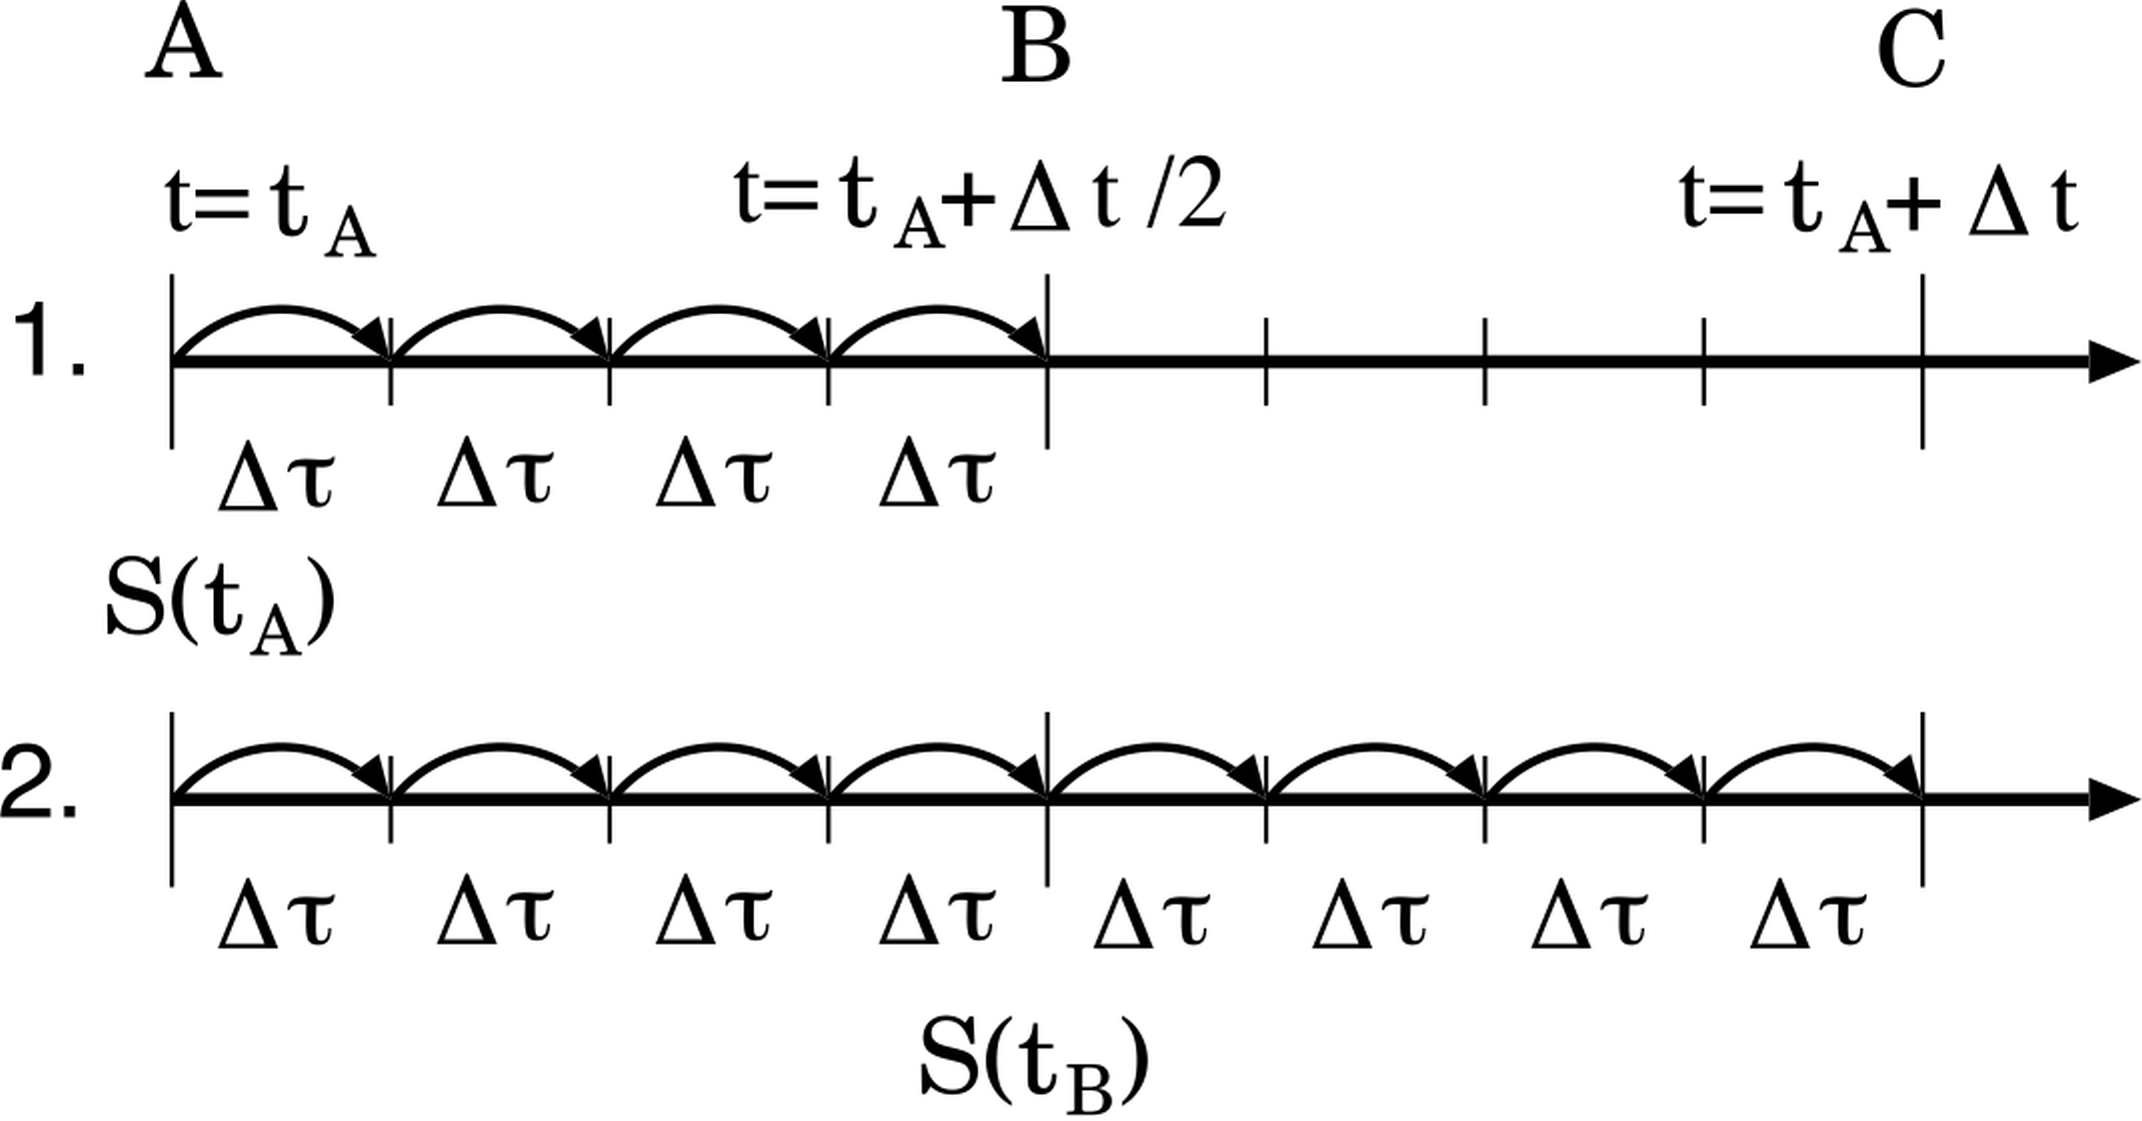
\includegraphics[scale=.3]{figs/Tomita1-20-0.png}
\caption{Schematic figure of temporal integration.}
\label{f:temporal_integration}
\end{figure}

If $\Psi$ at $t = t_A$ is given, the slow-mode tendency $S(t_A)$ can be
evaluated.
%
The variable is integrated from $t_A$ to $t_B (> t_A)$ using
%
$S(t_A) + F(t_A + m\Delta\tau)$ as the forcing function at $t=t_A +
m\Delta\tau$,
where $F(t_A + m\Delta\tau)$ is the fast-mode tendency being updated at
every small step and $m$ is the index of small time steps.
%
Repeating integration with this small step, the temporary value of the
prognostic variable $\Psi^*$ at $t_B$ can be obtained.
%
The slow-mode tendency $S(t_B)$ is evaluated using this value.
%
Finally, integrated variable $\Psi$ at $t=t_C(>t_B)$ is calcurated by
$S(t_B) + F(t_A + m\Delta\tau)$.



\section{Icosahedral grid and ``glevel''}\label{s:ico_grid_glevel}

To overcome the pole problem which old-fashioned global models have,
\NICAM uses the icosahedral grid system.
In this grid system, grid points are distributed quasi-homogeneously on
the sphere.
%
The icosahedral grid can be constructed by a recursive division method
which is similar to that of \cite{Stuhne:1996fr}.
%
The grid resolution obtained by $i$-th dividing operation is called
``glevel-$i$''.
%
First, vertices of the spherical icosahedron construct glevel-0 (
\autoref{f:glevel_0}).
%
By connecting the midpoint of each edge of the triangles, the next finer
grid glevel-1 is generated as \autoref{f:glevel_1}.
%
Doing the same procedure, glevel-2 is
generated(\autoref{f:glevel_2}).
%
For example, \autoref{f:glevel_5} shows the
glevel-5 grid.

\begin{figure}[tb]
\centering
\begin{subfigure}{.32\textwidth}
\centering
 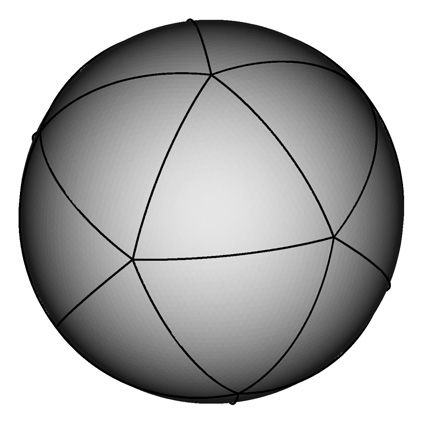
\includegraphics[width=\textwidth]{figs/Tomita_etal_2008_SIAM-7-0.png}
\caption{glevel=0}\label{f:glevel_0}
\end{subfigure}
\begin{subfigure}{.32\textwidth}
\centering
 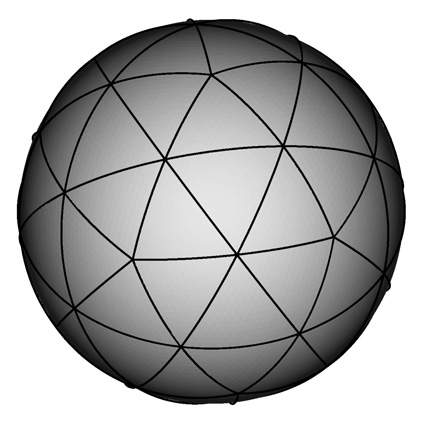
\includegraphics[width=\textwidth]{figs/Tomita_etal_2008_SIAM-7-1.png}
\caption{glevel=1}\label{f:glevel_1}
\end{subfigure}
\begin{subfigure}{.32\textwidth}
\centering
 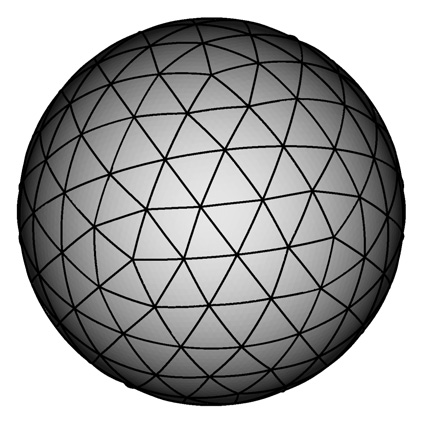
\includegraphics[width=\textwidth]{figs/Tomita_etal_2008_SIAM-7-2.png}
\caption{glevel=2}\label{f:glevel_2}
\end{subfigure}
\caption{The method of horizontal grid refinement.}\label{f:horiz_grid_refinement}%\label{195813_22Oct17}
\end{figure}

\begin{figure}[tb]
\centering
 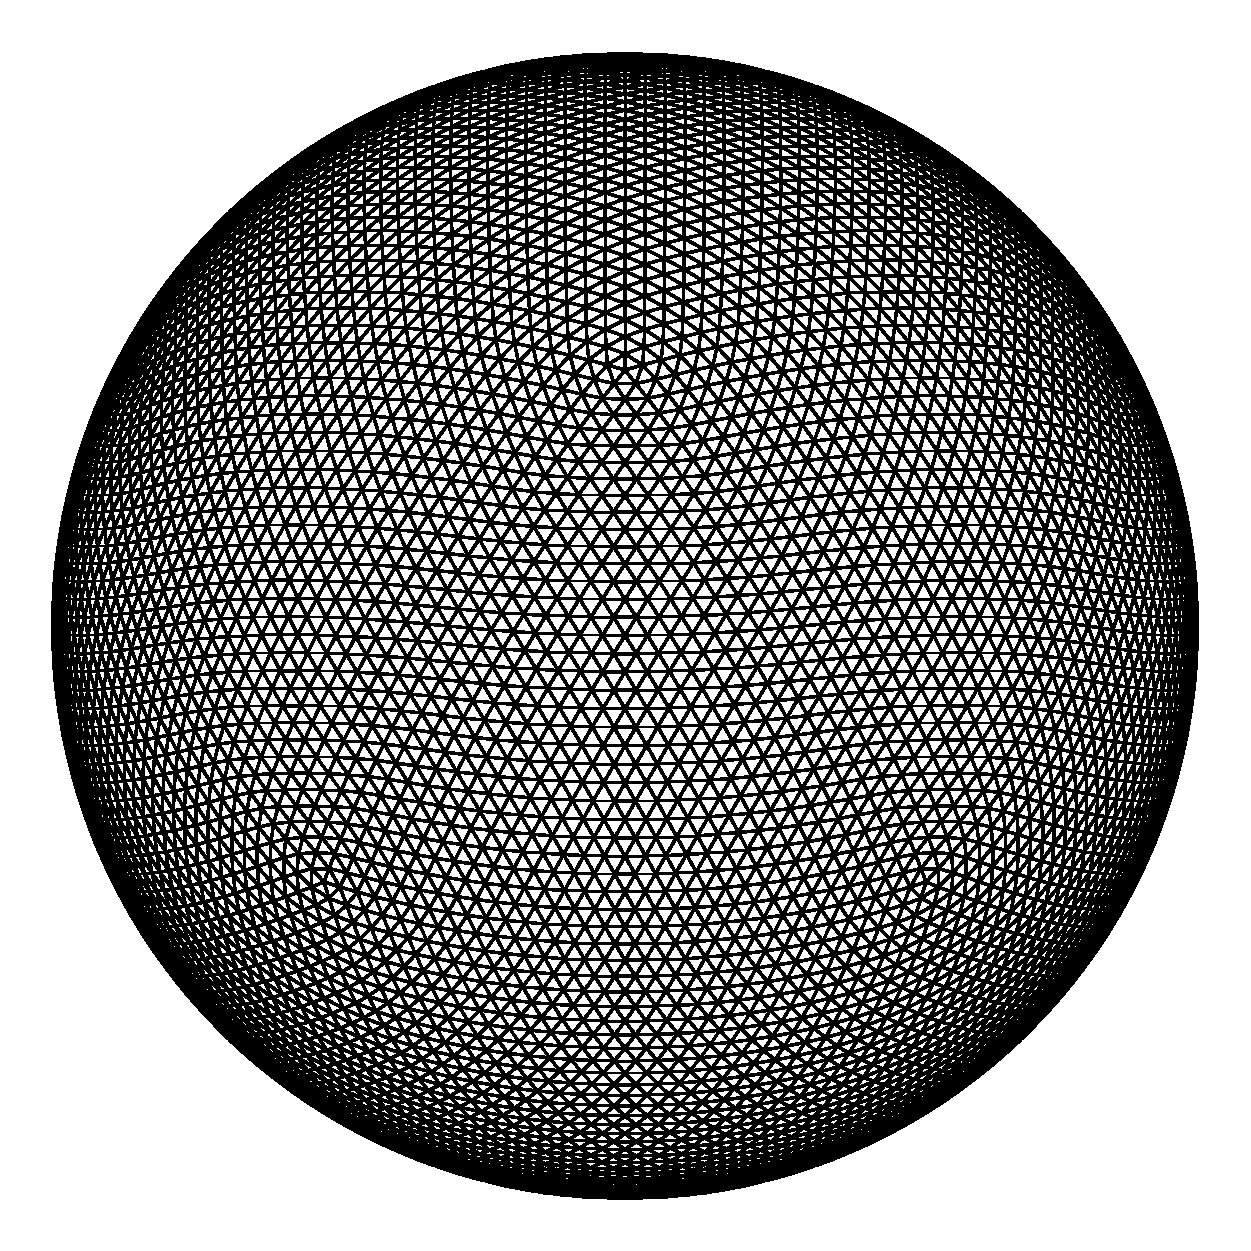
\includegraphics[scale=.25]{figs/Tomita1-26-0.png}
 \caption{The icosahedral grid with glevel-5}
 \label{f:glevel_5}
\end{figure}


All the variables are defined at the vertices of triangular grid
elements.
%
This arrangement is categorized into the Arakawa-A type grid.
%
The control volume is defined as the polygon constructed by connecting
the gravitational centers of neighboring triangular grid elements.
%
The shape of control volume is hexagon, as shown in 
\autoref{f:control_volume}, except that it is pentagon at only twelve points
inherited from the original icosahedron.

\begin{figure}[tb]
 \centering
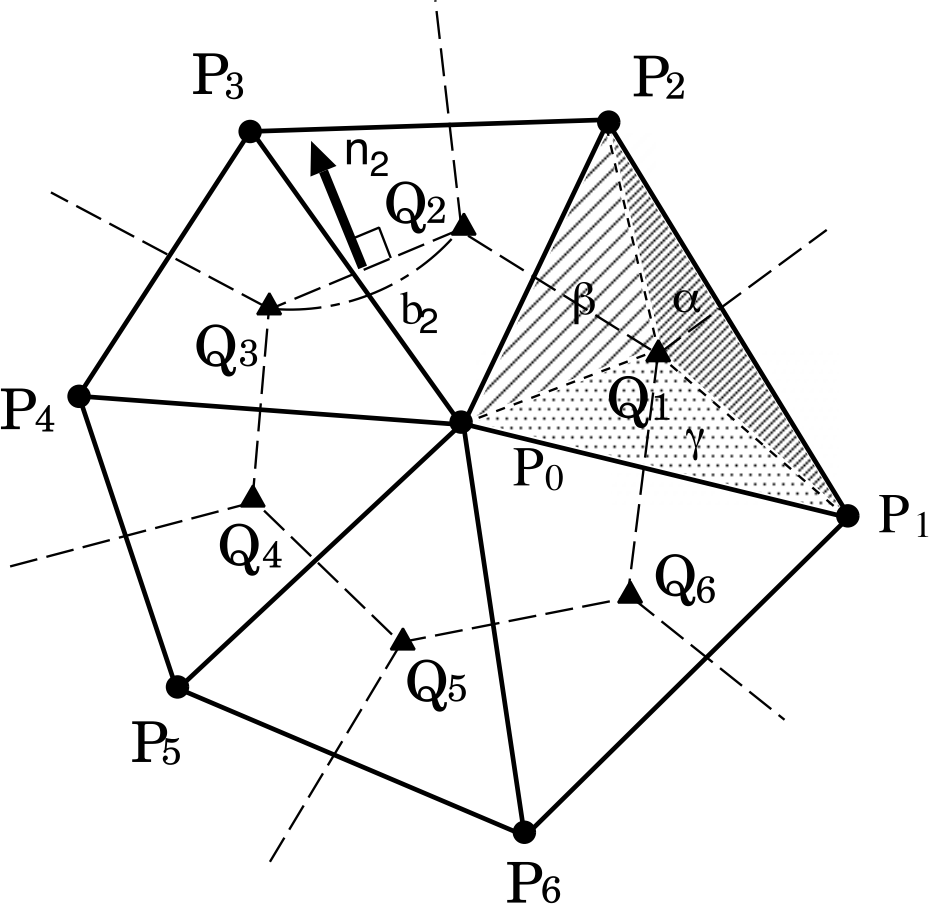
\includegraphics[scale=0.7]{figs/Tomita1-27-0.png}
 \caption{Schematic figure of control volume. \citep{Tomita:2008jc}}
 \label{f:control_volume}
\end{figure}


\NICAM adopts the finite volume method for the discretization of
differential operators.
%
In \autoref{f:control_volume}, some vector $\bm{u}$
at the vertices of control volume $Q_i$ are calculated by interpolation
as\footnotemark
%
\footnotetext{$P_{i+1}$ should be $P_{1+\text{mod}{(i,6)}}$, and the same hereinafter.}
%
\begin{equation}
 \bm{u} (Q_i) \simeq
 \frac{\alpha \bm{u}(P_0) + \beta \bm{u}(P_i) + \gamma \bm{u}(P_{i+1})}
      {\alpha + \beta + \gamma} ,\label{e:u_Q_i}
\end{equation}
%
where $\alpha$, $\beta$ and $\gamma$ are the areas of the triangle
$Q_i P_i P_{i+1}$, $Q_0 P_{i+1} P_0$ and $Q_i P_0 P_i$, respectively.
%
The number 6 is replaced with 5 at the pentagonal control volumes for
the singular points.

The divergence is calculated from the Gauss theorem as
%
\begin{equation}
 \nabla \cdot \bm{u}(P_0) \simeq \frac{1}{a(P_0)} %
  \sum^{6}_{i=1} b_i \frac{\bm{u}(Q_i)+\bm{u} (Q_{i+1})}{2} \cdot
  \bm{n}_i,\label{e:nabla_u_P_0}
\end{equation}
%
where $b_i$ and $\bm{n}_i$ denote the geodesic arc length of
$Q_i Q_{i+1}$ and the outward unit vector normal to this arc at the
midpoint of $Q_i Q_{i+1}$.
%
$a(P_0)$ is the area of control volume at the point $P_0$.
%
More than that, \autoref{e:nabla_u_P_0} can be rewritten as a
linear combination:
%
\begin{equation}
 \nabla \cdot \bm{u} (P_0) = \sum^{6}_{i=1} \bm{c}_i \cdot \bm{u}(P_i)\label{e:nabla_u_P_0_eq}
\end{equation}
%
where $\bm{c}_i$ are constant vector coefficients which can be
pre-calculated once and stored for subsequent use.
%
In \autoref{e:nabla_u_P_0_eq}, the number of addition and
multiplication is the same, this formulation is preferable for the CPU
which has FMA.



The gradient operator to an arbitrary variable $\phi$ is calculated as

\begin{equation}
 \nabla \phi(P_0) \simeq
  \frac{1}{a(P_0)}
  \sum^{6}_{i=1} b_i \frac{\phi(Q_i) + \phi(Q_{i+1})}{2} \bm{n}_i
  - \frac{\phi_0}{a(P_0)} \sum^{6}_{i=1} b_i \bm{n}_i,\label{e:nabla_phi_P_0}
\end{equation}
%
where $\phi(Q_i)$ is interpolated by the similar way to the 
\autoref{e:u_Q_i}.
%
This scheme given as \autoref{e:nabla_phi_P_0} generates the
vertical component because the allocation points are on the sphere.
%
In practice, the vertical component is removed after the operation of
\autoref{e:nabla_phi_P_0}.


More precisely, \NICAM used modified icosahedoral grid by using spring dynamics in order to avoid
severe problems on the numerical accuracy and stability.
See \cite{Tomita:2001id} for the details.
%


\section{Upwind-Biased Advection Scheme}\label{s:upwind_scheme}

\NICAM uses an upwind-biased advection scheme for icosahedral grid
derived by \cite{Miura:2007bs}.
%
\autoref{f:2007mwr2101_1-0} (a) shows arrangement of distorted hexagonal
cells. Computational nodes are $\bm{P}_i(i=0,2,...,6)$, hexagonal cell
corners are $\bm{Q}_i$, center of hexagonal cell faces are $\bm{R}_i$,
lengths of hexagonal cell faces are $l_i$, and unit vectors normal to
cell faces are $\bm{n}_i$.
%
\autoref{f:2007mwr2101_1-0} (b) shows schematic of the area swept by the
arc $\bm{Q}'_i\bm{Q}'_{i+1}$ during a time interval.
%
Here we assumes that the arc $\bm{Q}'_i\bm{Q}'_{i+1}$ at time $t$
moves with a constant velocity $\bm{v_R}^{t+\Delta t/2}$
and concides with the arc $\bm{Q}_i\bm{Q}_{i+1}$ at time $t+\Delta t$.
%
The total amount of flux through the edge $\bm{Q}_i\bm{Q}_{i+1}$
during the time interval $\Delta t$ is approximated by the amount of a
tracer inside the parallelogram
$\bm{Q}'_i\bm{Q}'_{i+1}\bm{Q}_{i+1}\bm{Q}_i$,
%
Profiles of $\rho$ and $q$, he density and the
tracer mixing ratio, respectively, inside this parallelogram can be
approximated by two-dimensional linear surface.
%
Then the amount of a tracer inside this parallelogram is
%
\begin{equation}
\rho_{\bm{R}_i} q_{\bm{R}_i} 
 = \frac{\int_{S_i} \rho q \ \mathrm{d}S}
         {S_i}  
 = \rho_{\bm{C}_i} q_{\bm{C}_i},
\end{equation}
%
where $S_i$ and 
$\bm{C}_i$ denotes the area and the mass centroid of this parallelogram, respectively.
%
Similarly, the continuity equation will yield
%
\begin{equation}
 \rho_{\bm{R}_i} = \rho_{\bm{C}_i}.
\end{equation}
%
Thus,
%
\begin{equation}
 q_{\bm{R}_i} = q_{\bm{C}_i}.
\end{equation}
%
The position of $\bm{C}_i$ can be computed as
%
\begin{equation}
\bm{C}_i = \bm{R}_i - v_{\bm{R}_i}^{t+\Delta t/2} \frac{\Delta t}{2}.
\end{equation}
%
Linear surfaces inside the parallelogram can be approximated by nodal
values and gradients at a computational node that shares the cell face
and is on the upwind side of the cell face.
%
See \cite{Miura:2007bs} for more details.

\begin{figure}[htbp]
\centering
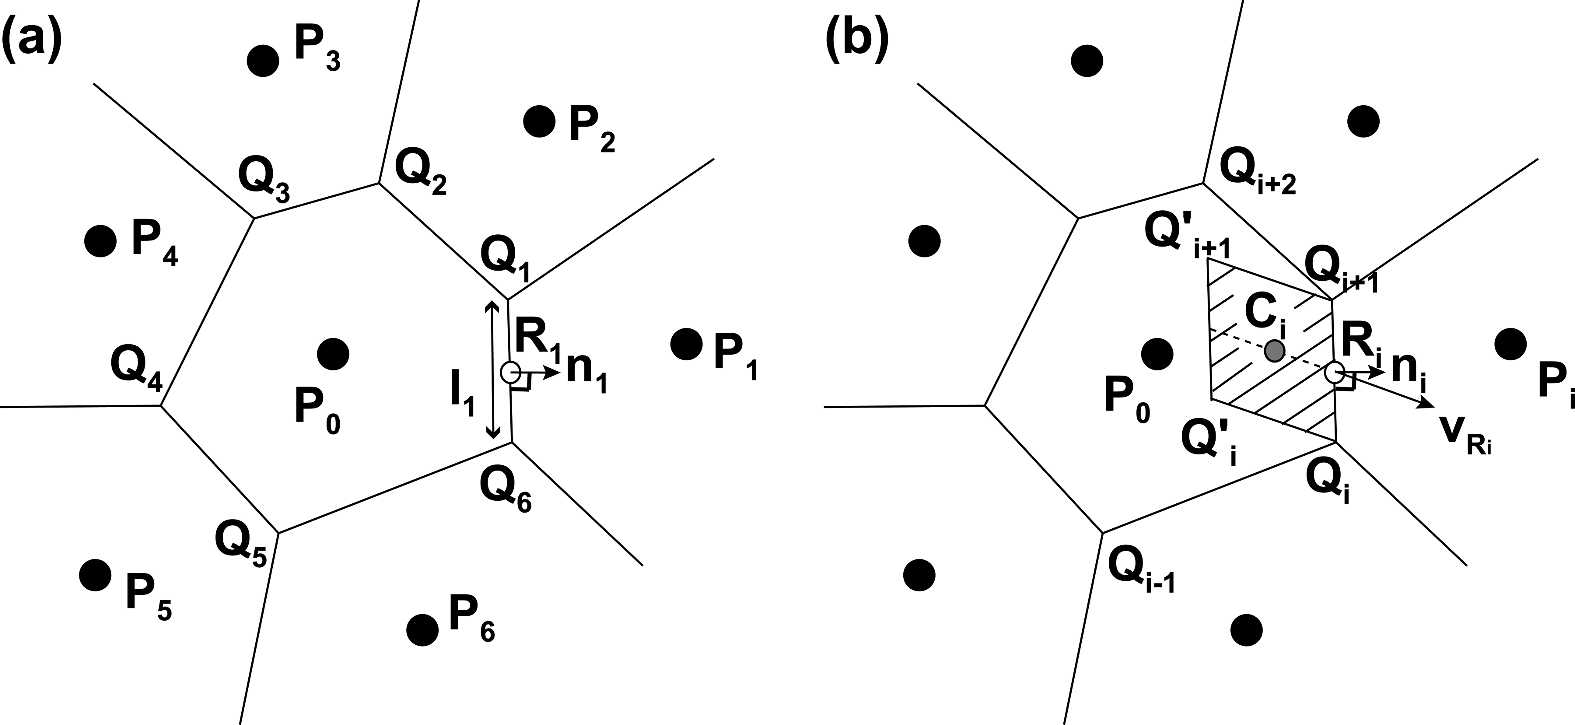
\includegraphics[scale=.3]{figs/2007mwr2101_1-0.png} 
 \caption{%
(a) Arrangement and notation of distorted hexagonal cells.%
(b) Schematic of the area swept by the arc $\bm{Q}'_i \bm{Q}'_{i+1}$ during a time interval.%
}\label{f:2007mwr2101_1-0}
\end{figure}


\section{Vertical coordinate and discretization}\label{s:vert_coord}

\NICAM uses the Lorenz grid for the vertical grid configuration as shown
in \autoref{f:vert_grid_config},
where $W$ (vertical velocity with metrics) is defined at the
half-integer levels and the other variables are defined at the integer
levels.
%
This model allows the grid stretching in the $\xi$ coordinate as show in
\autoref{f:vert_grid_config}.
%
The integer levels are located at the mid-point of the upper and lower
half-integer levels.
%
The linear interpolation is used to obtain the values at the
half-integer levels from the values at the integer levels, and vice
versa:
%
\begin{align}
 \phi_{k+1/2} &= a_{k+1/2}\, \phi_{k+1} + b_{k+1}\,\phi_k,\\
 \phi_k       &= c_k \, \phi_{k+1/2} + d_k \, \phi_{k-1/2},
\end{align}
%
where
%
\begin{align}
 a_{k+1/2} &= \frac{\xi_{k+1/2} - \xi_k}{\xi_{k+1}-\xi_k},\\
 b_{k+1/2} &= 1 - a_{k+1/2} ,\\
 c_k       &= \frac{\xi_k - \xi_{k-1/2} }{\xi_{k+1/2} - \xi_{k-1/2}},\\
 d_k       &= 1 - c_k.\\
\end{align}


\begin{figure}[tb]
\centering
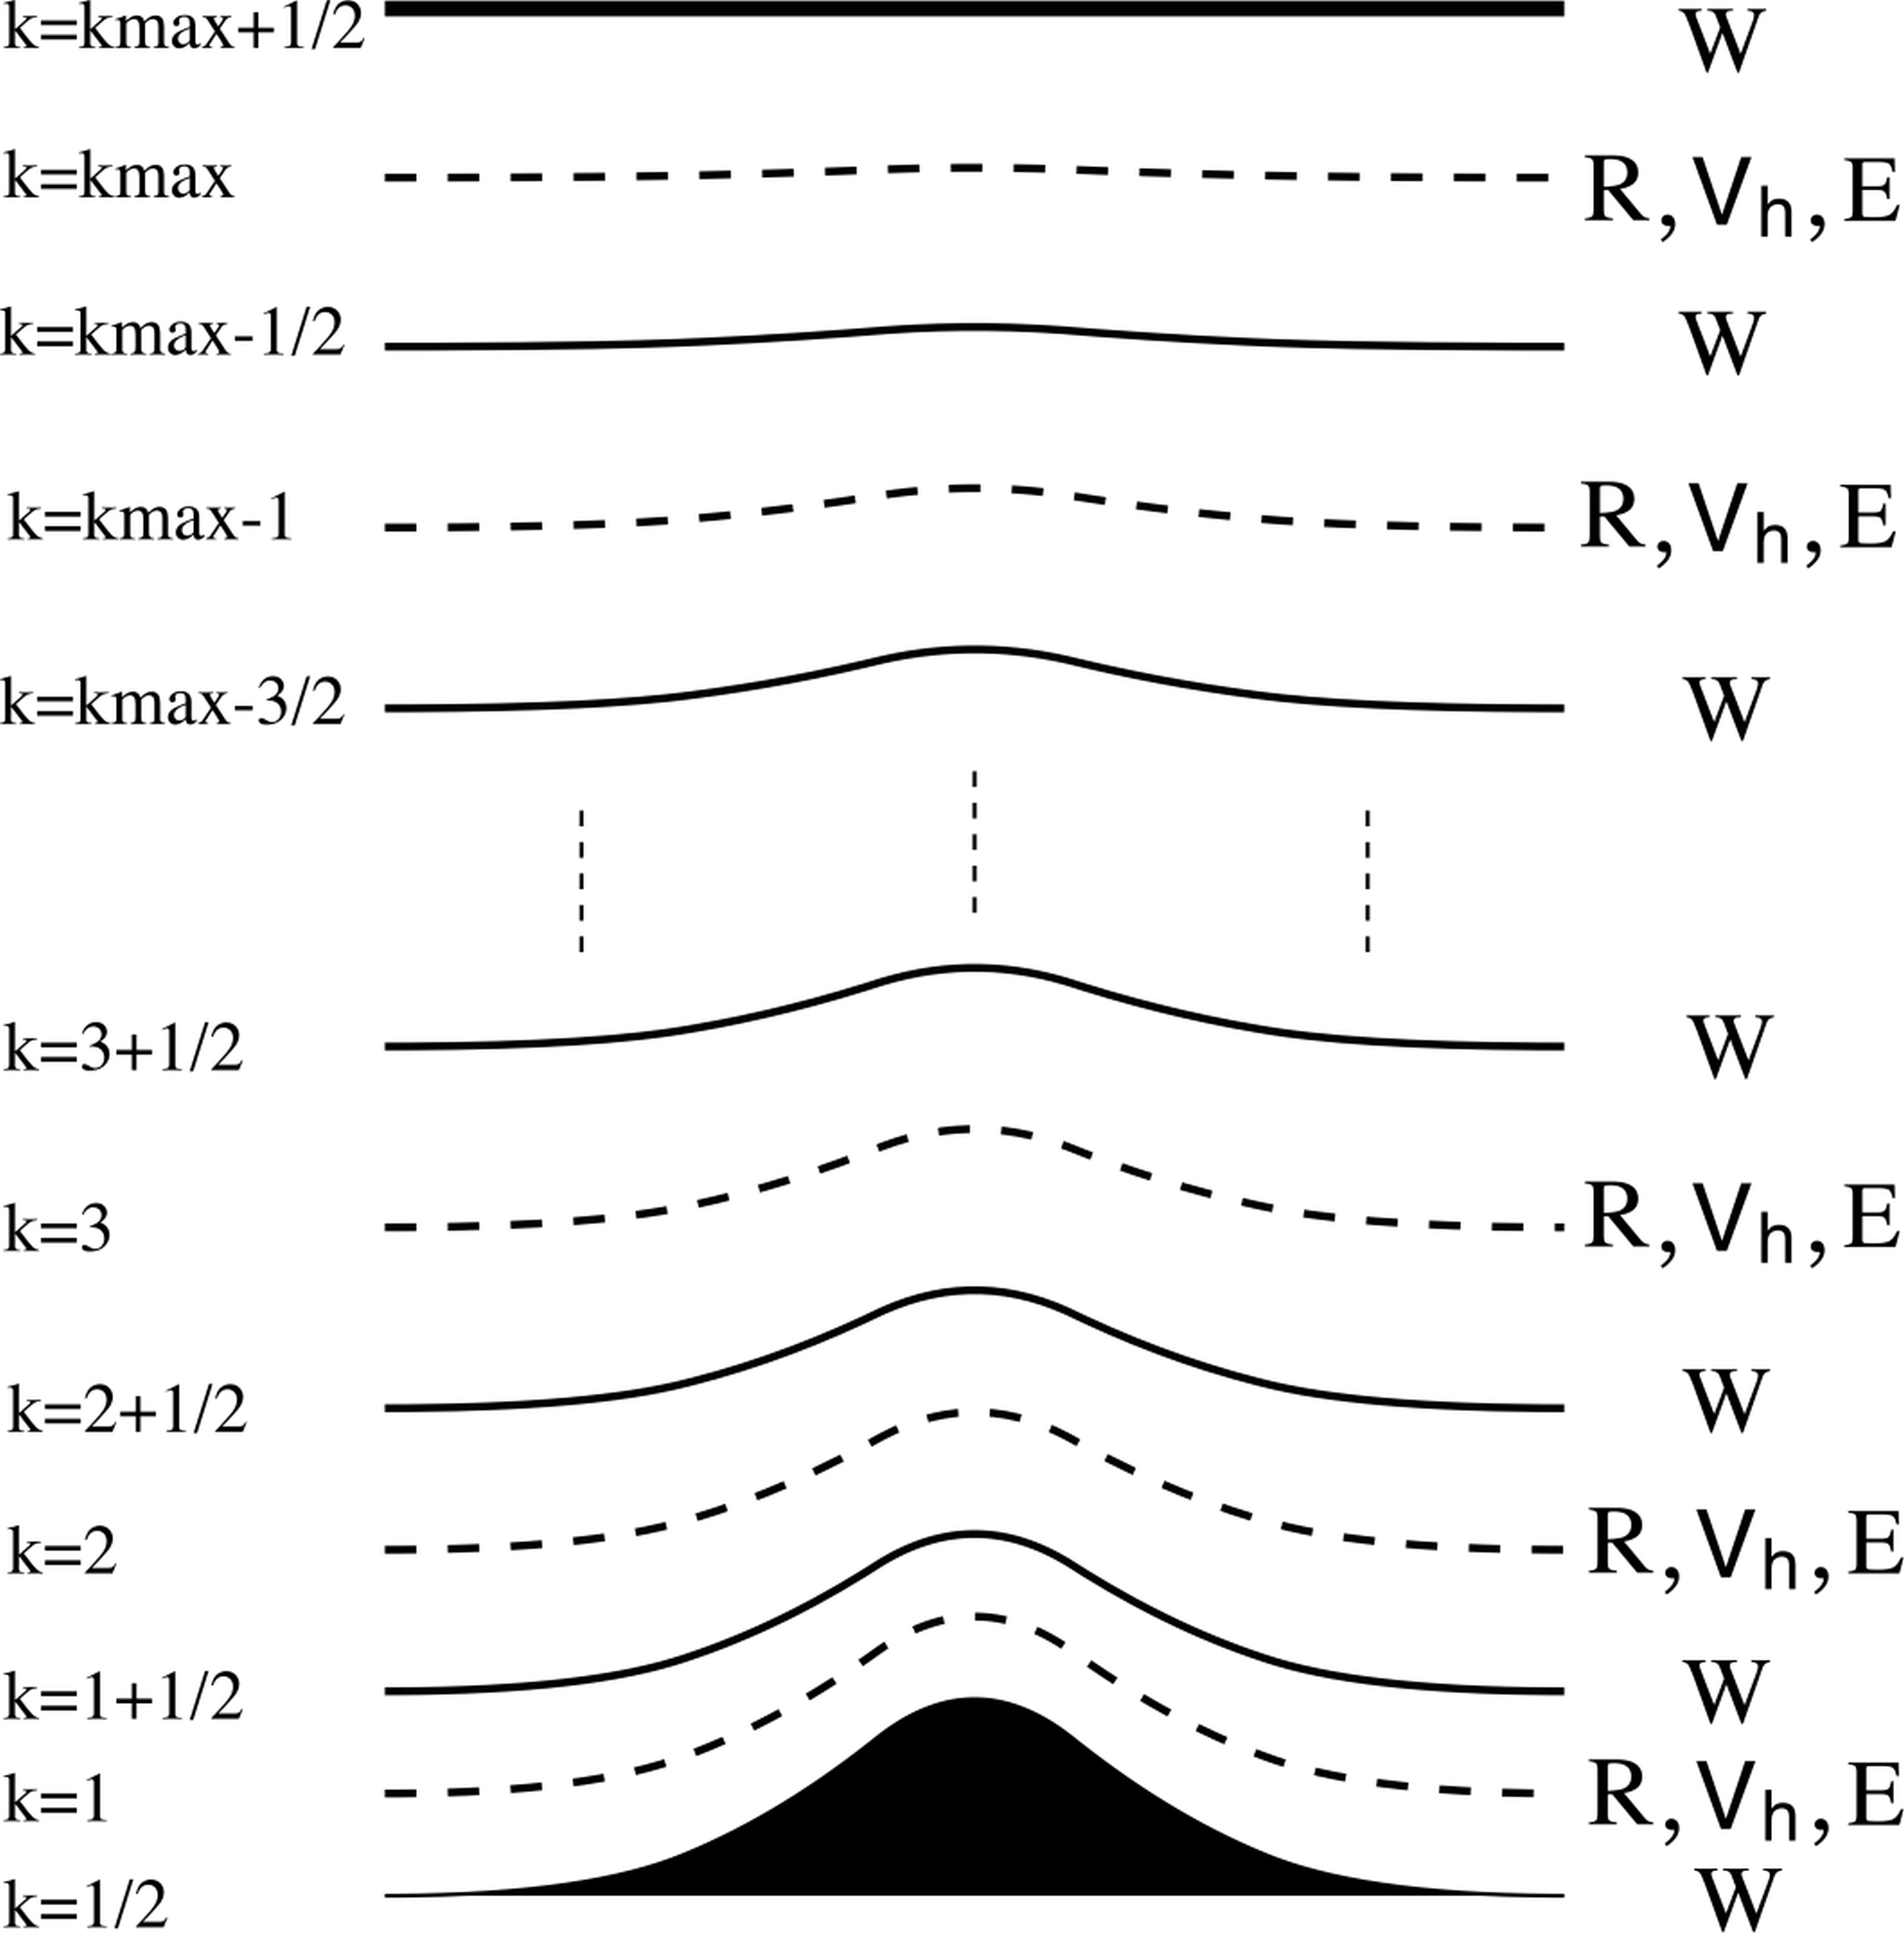
\includegraphics[scale=.4]{./figs/Tomita1-23-1.png}
\caption{Schematic figure of vertical grid configuration.}
\label{f:vert_grid_config}
\end{figure}


One of main solvers is that of the Helmholtz equation, which can be
expressed as
%
\begin{equation}
 - \frac{\partial}{\partial\xi}
 \left[ A^o \frac{\partial(A^i\tilde{W})}{\partial\xi} \right]
 - \frac{\partial(B\tilde{W})}{\partial\xi}
 - C^o \frac{\partial C^i\tilde{W}}{\partial\xi}
 + \alpha D \tilde{W} = S^\text{all}
\label{e:helmholtz_eq}
\end{equation}
%
where
%
\begin{equation}
 \tilde{W} \equiv \frac{{W^* }^{\tau + \Delta \tau}  }{G^{1/2} \gamma^2}
 \left( = {(\rho w)^* }^{\tau + \Delta \tau}\right)
\end{equation}
%
and the coefficients are given as
%
\begin{align}
 A^o &= \frac{1}{G^{1/2}\gamma^2},\\
 A^i &= \gamma^2 h^t,\\
 B   &= \tilde{g}^t, \\
 C^o &= \frac{C_v g}{R_d \gamma^2},\\
 C^i &= \gamma^2, \\
 D   &= \frac{C_v G^{1/2}}{R_d \Delta \tau ^2}.
\end{align}

The source term is given as
\begin{equation}
 S^\text{all} = \frac{C_v}{R_d \Delta \tau^2}
  \left(\frac{\alpha{W^*}^\tau+\Delta \tau S^W}{\gamma^2}
   -\Delta \tau \frac{\partial}{\partial\xi}
   \left[ \frac{1}{G^{1/2}\gamma^2}({P^*}^\tau + \Delta \tau S^P) \right]
-\frac{\Delta \tau}{\gamma^2}({R^*}^\tau + \Delta \tau S^R)g
\right).
\end{equation}
%
\autoref{e:helmholtz_eq} is in discretized form at the level
$k+1/2$:

\begin{align}
&- \left[
    \frac{A^o_{k+1}\left(A^i_{k+3/2}\tilde{W}_{k+3/2}
                    -    A^i_{k+1/2}\tilde{W}_{k+1/2}\right)}
         {\Delta\xi_{k+1}\Delta\xi_{k+1/2}}
   - \frac{A^o_k\left(A^i_{k+1/2}\tilde{W}_{k+1/2}
                -    A^i_{k-1/2}\tilde{W}_{k-1/2} \right)}
         {\Delta\xi_k\Delta_{k+1/2}}
   \right] \nonumber \\
 %
&- \left[
    \frac{\left( c_{k+1} B_{k+3/2}\tilde{W}_{k+3/2}
               + d_{k+1} B_{k+1/2}\tilde{W}_{k+1/2} \right)
    -     \left( c_k B_{k+1/2}\tilde{W}_{k+1/2}
           +     d_k B_{k-1/2}\tilde{W}_{k-1/2} \right)
    }
    {\Delta\xi_{k+1/2}}
  \right] \nonumber \\
 %
&- C^o_{k+1/2} \left[ \frac{\left(c_{k+1} C^i_{k+3/2} \tilde{W}_{k+3/2}
                               + d_{k+1} C^i_{k+1/2} \tilde{W}_{k+1/2}\right)
                         - \left(c_k C^i_{k+1/2}\tilde{W}_{k+1/2}
                               + d_k C^i_{k-1/2}\tilde{W}_{k-1/2}   \right)  }
                         {\Delta \xi_{k+1/2}}\right] \nonumber \\
 %
&+ \alpha D_{k+1/2} \tilde{W}_{k+1/2} \nonumber \\
&= S^{\text{all}}_{k+1/2}
\label{e:helmholtz_eq_discre}
\end{align}
%
where
%
\begin{align}
 S^\text{all}_{k+1/2}
= & \frac{C_v}{R_d \Delta \tau^2}
\left[
 \left(
  \frac{\alpha {W^*}^{\tau}_{k+1/2} + \Delta \tau S^W_{k+1/2}}
       {\gamma_{k+1/2}^2}
 \right)\right. \nonumber\\
&  - \frac{\Delta \tau}{\Delta \xi_{k+1/2}}
\left.
 \left(
  \frac{{P^*}^\tau_{k+1}+\Delta\tau S^P_{k+1}}{G^{1/2}_{k+1}
       {\gamma_{k+1}}^2}
 -\frac{{P^*}^\tau_k + \Delta\tau S^P_k}
       {G^{1/2}_k \gamma_k^2}
 \right)\right. \nonumber\\
&  - g\Delta\tau
\left.
  \left(
   a_{k+1/2}\frac{{R^*}^\tau_{k+1}+\Delta\tau S^R_{k+1}}{\gamma_{k+1}^2}
+  b_{k+1/2}\frac{{R^*}_k^\tau + \Delta\tau S^R_k}{\gamma_k^2}
  \right)
\right]
\end{align}
%
\autoref{e:helmholtz_eq_discre} is a tridiagonal matrix system as follows:
%
\begin{equation}
 \begin{gathered}
  M^L_{k+1/2}\tilde{W}_{k-1/2}
+ M^C_{k+1/2}\tilde{W}_{k+1/2}
+ M^U_{k+1/2}\tilde{W}_{k+3/2}
= S^\text{all}_{k+1/2}, \\
\text{for}  \quad \frac{3}{2} \leq k+\frac{1}{2} \leq k_\text{max} -\frac{1}{2},
 \end{gathered}
\end{equation}
%
where
%


\begin{align}
 M^C_{k+1/2} = & \quad \alpha D_{k+1/2} \nonumber\label{e:M^C}\\
               & + \frac{1}{\Delta\xi_{k+1/2}}
 \left[
   \frac{A^o_{k+1} A^i_{k+1/2}}{\Delta\xi_{k+1}}
 + \frac{A^o_k A^i_{k+1/2}}{\Delta\xi_k}
 - (d_{k+1}-c_k)(B_{k+1/2}+C^o_{k+1/2} C^i_{k+1/2})
 \right],\\
 %
 M^U_{k+1/2} = &
 - \frac{A^o_{k+1} A^i_{k+3/2}}
        {\Delta\xi_{k+1}\Delta\xi_{k+1/2}}
 - \frac{c_{k+1}(B_{k+3/2}+C^o_{k+1/2} C^i_{k+3/2} )}
 {\Delta\xi_{k+1/2}} ,\label{e:M^U}\\
 %
 M^L_{k+1/2} = &
 -\frac{A^o_{k+1}A^i_{k-1/2}}{\Delta\xi_{k+1}\Delta\xi_{k+1/2}}
 +\frac{d_k(B_{k-1/2}+C^o_{k+1/2}C^i_{k-1/2})}{\Delta\xi_{k+1/2}} .\label{e:M^L}
\end{align}
%
If the boundary conditions for $\tilde{W}$ are given at $k=1-1/2$ and
$k_\text{max} + 1/2$, this linear system can be written explicitly as
%

\begin{equation}
\begin{gathered}
  \begin{pmatrix}
 M^C_{1+1/2} & M^U_{1+1/2} & 0 & \cdots & \cdots & \cdots & 0 \\
 M^L_{2+1/2} & M^C_{2+1/2} & M^U_{2+1/2}& 0 & \cdots& \cdots& \vdots \\
  0 & M^L_{3+1/2} & M^C_{3+1/2} & M^U_{3+1/2} & 0 & \cdots & \vdots \\
  \vdots & & \cdots & \cdots & \cdots & & 0\\
  \vdots & \cdots & \cdots & 0 & M^L_{k_\text{max}-3/2}  &M^C_{k_\text{max}-3/2} & M^U_{k_\text{max}-3/2} \\
  0 & \cdots & \cdots & \cdots & 0 & M^L_{k_\text{max}-1/2} &  M^C_{k_\text{max}-1/2} \\
  \end{pmatrix}\\
 \times
  \begin{pmatrix}
   \tilde{W}_{1+1/2}\\
   \tilde{W}_{2+1/2}\\
   \tilde{W}_{3+1/2}\\
   \vdots\\
   \tilde{W}_{k_\text{max}-3/2}\\
   \tilde{W}_{k_\text{max}-1/2}\\
  \end{pmatrix}
  =
  \begin{pmatrix}
   S^\text{all}_{1+1/2} - M^L_{1+1/2} \tilde{W}_{1-1/2}\\
   S^\text{all}_{2+1/2}\\
   S^\text{all}_{3+1/2}\\
   \vdots\\
   S^\text{all}_{k_\text{max}-3/2}\\
   S^\text{all}_{k_\text{max}-1/2} - M^U_{k_\text{max}-1/2}\tilde{W}_{k_\text{max}+1/2}
  \end{pmatrix}
\end{gathered}\label{e:linear_system_explicitly}
\end{equation}
%
Since $A^i$ and $B$ depend on large step values(see \autoref{s:time_integration}), the
compositions of the matrix (\autoref{e:M^C},
\ref{e:M^U}, \ref{e:M^L}, \ref{e:linear_system_explicitly}) are
the updated only at the large step.


\section{Domain decomposition and ``rlevel''}
% Tomita_etal_2008_SIAM Sec3.1

For domain decomposition for parallel computing, \NICAM adopt the
concept of a region-division level, or ``rlevel'', along with the
grid-division level \citep{Tomita:2008jc}.
%
The ten rectangles in \autoref{f:rlevel=0} are the
result of connecting two neighboring triangles of a spherical
icosahedron.
%
This structure is called ``rlevel-0''.
%
For each rectangle, four subrectangles are generated by connecting the
diagonal midgridpoints (\autoref{f:rlevel=1}).
%hu
This structure is called ``rlevel-1''.
%
This process is repeated until the desired number of regions is
obtained.



\begin{figure}[htb]
\centering
\begin{subfigure}{.3\textwidth}
\centering
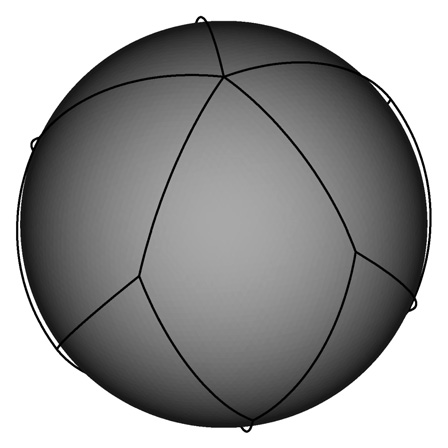
\includegraphics[width=\textwidth]{figs/Tomita_etal_2008_SIAM-8-0.png}
\caption{rlevel=0}\label{f:rlevel=0}
\end{subfigure}
\begin{subfigure}{.3\textwidth}
\centering
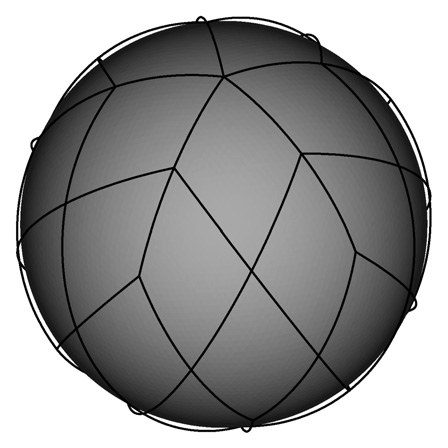
\includegraphics[width=\textwidth]{figs/Tomita_etal_2008_SIAM-8-1.png}
\caption{rlevel=1}\label{f:rlevel=1}
\end{subfigure}
\begin{subfigure}{.3\textwidth}
\centering
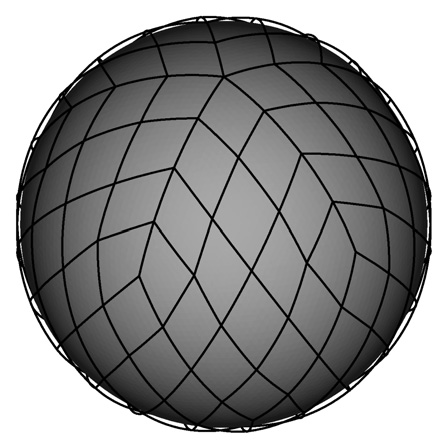
\includegraphics[width=\textwidth]{figs/Tomita_etal_2008_SIAM-8-2.png}
\caption{rlevel=2}
\end{subfigure}
\caption{The method of region division. \citep{Tomita:2008jc}}%
 \label{f:region_division}
\end{figure}



\section{Horizontal data structure}\label{s:horiz_data_structure}

% Tomita_etal_2008_SIAM

As described in \autoref{s:ico_grid_glevel}, the grid elements of an
icosahedral grid are not rectangles.
%
In \NICAM, the shape of the control volume is hexagonal, except for the 12 points
associated with the original icosahedron vertices.
%
Therefore, the icosahedral grid is categorized as an unstructured
grid.
%
However, an icosahedral grid can actually be treated as a structured grid.
%
An example of the grid structure in a region is shown in \autoref{f:normal_region}.
%
The memory of each region in a single layer can be stored as a continuous one- or two-dimensional array.
%
In \autoref{f:normal_region}, the region manages the black gridpoints.
%
The values indicated by the white circles are used only for reference
and are provided from the neighboring regions by communication or memory
copy.
%
The values at the red circles are not used.
%
If the west vertex of a region corresponds to a vertex of the original
icosahedron, the two blue points shown in \autoref{f:normal_region}
have the same values.
%
With this data configuration, the black points cover all the icosahedral
grid points except for the north and south poles.

\autoref{f:pole_region} shows data storage for the pole-region
data.
%
The gridpoint value included in this region is marked by a black
circle.
%
The other values marked by white circles are reference values, provided
by communication or memory copy from the neighboring regular regions.
%
The indices of the reference points are given in clockwise order.
%
The pole regions are managed by the master process.
%
Although this might cause load imbalance in parallel computing, the
ratio of calculation required at the poles to that required in regular
regions is small, and in practice the problem is negligible.

\begin{figure}[htb]
 \begin{subfigure}[t]{.45\textwidth}
  \centering
  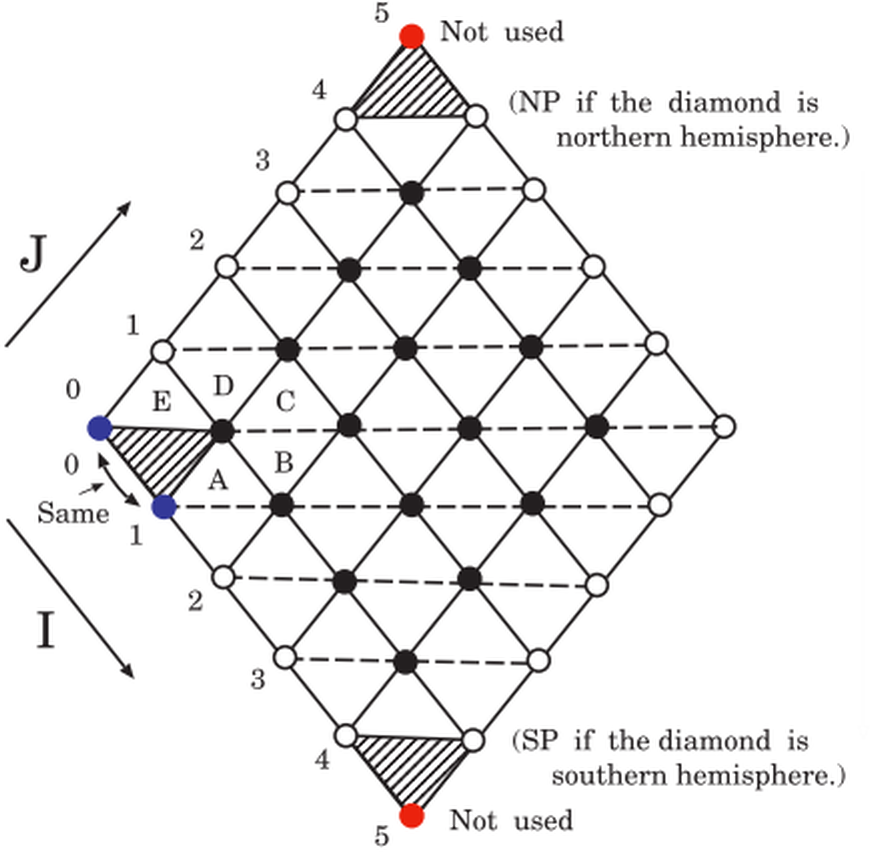
\includegraphics[width=\textwidth]{figs/Tomita_etal_2008_SIAM-9-0.png}
  \caption{Normal region}\label{f:normal_region}
 \end{subfigure}
 \begin{subfigure}[t]{.45\textwidth}
  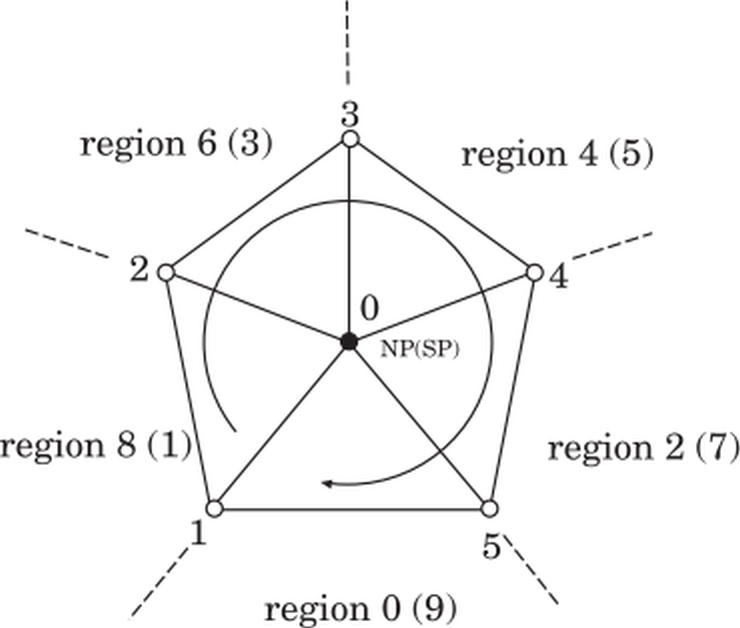
\includegraphics[width=\textwidth]{figs/Tomita_etal_2008_SIAM-9-1.png}
  \caption{Pole region}\label{f:pole_region}
 \end{subfigure}
\caption{Grid structure of a region.\citep{Tomita:2008jc}}
\label{f:grid_structure_of_a_region}
\end{figure}


\section{Parallelization}

%Tomita_etal_2008_SIAM

\NICAM uses MPI for parallel execution.
%
One MPI process manages one or several regions defined in previous
section.
%
For regions managed by the same process, exchanges of boundary values
are done by memory copy, otherwise done by MPI communication.
%
\autoref{f:parallellization} shows a schematic diagram of region
management.
%
In this case, rlevel is 1 and there are 40 regions, managed by 10 MPI
processes.
%
So a single process manages 4 regions, shown by the same color.

\begin{figure}[htb]
\centering
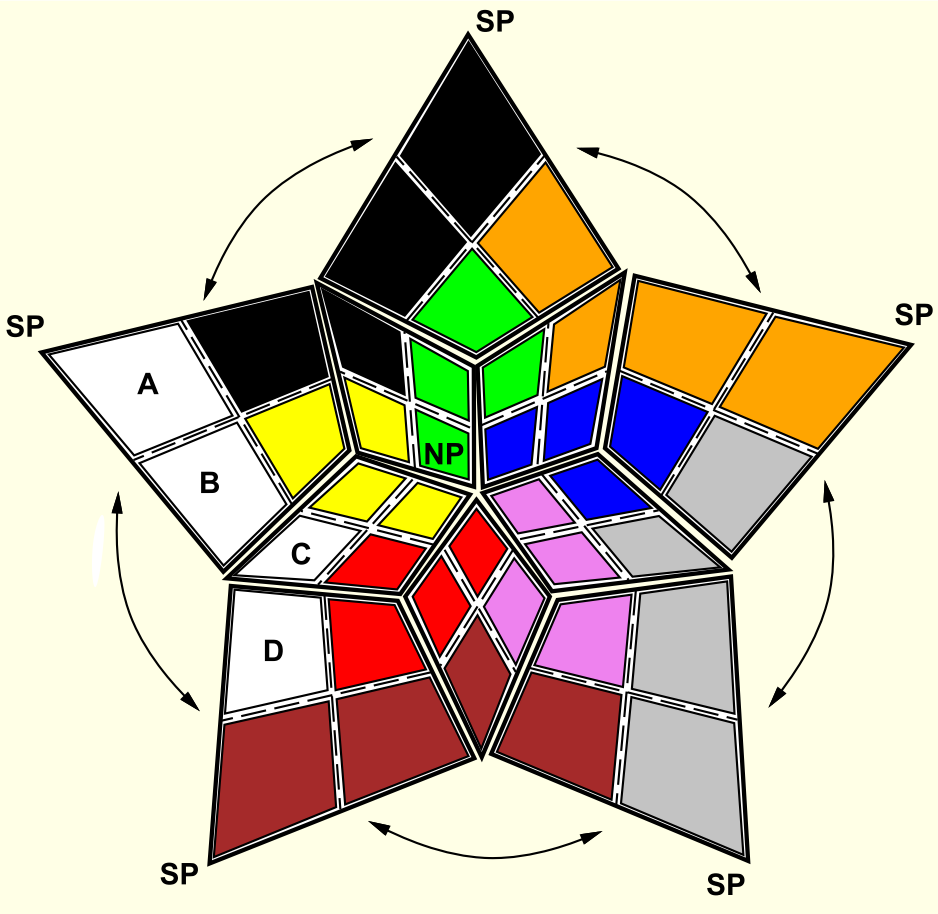
\includegraphics[scale=.7]{figs/Tomita2-10-0.png}
\caption{Schematic figure of parallelization. This figure shows the expansion of region geometry
with rlevel-1.}
\label{f:parallellization}
\end{figure}

\section{Problem size}

As shown in \autoref{s:ico_grid_glevel}, total number of grid points
are defined by glevel.
%
Total grid points $N_g$ is calculated by \autoref{e:N_g}.
%
\begin{equation}
 N_g = 10 \times 4^\text{gl} + 2, \label{e:N_g}
\end{equation}
%
where $\text{gl}$ is glevel. $+ 2$ is corresponding to the pole points.
%
\autoref{t:num_of_grid_points_and_glevel} shows total number of grid points and average
grid point distance for several
glevels.


\begin{table}[htb]
\centering
\caption{Number of grid points and glevel}
\label{t:num_of_grid_points_and_glevel}
\small
\begin{tabular}{|r|r|r|}
\hline
glevel& grid points & average grid interval[\si{\meter]}\\
\hline
 0&  \num{12}&         \num{7142126}\\
\hline
 1&  \num{42}&         \num{3571063} \\
\hline
 2&  \num{162}&        \num{1785432} \\
\hline
 $\cdots$ & $\cdots$& $\cdots$\\
\hline
 8&  \num{655362}&     \num{27899}\\
\hline
 9&  \num{2621442}&    \num{13949}\\
\hline
 10& \num{10485762}&   \num{6975}\\
\hline
 11& \num{41943042}&   \num{3487}\\
\hline
$\cdots$ & $\cdots$& $\cdots$\\
\hline
 13& \num{2684354562}& \num{872}\\
\hline
\end{tabular}
\end{table}


Similary, Total number of regions $N_r$is calculated by \autoref{183551_22Oct17}.
%
\begin{equation}
 N_r = 10 \times 4^\text{rl}, \label{183551_22Oct17}
\end{equation}
%
where $\text{rl}$ is rlevel.
%
\autoref{t:num_of_regions_and_rlevel} shows the relation of rlevel and number of regions.

\begin{table}[htb]
\centering
\caption{Number of regions and rlevel}
\label{t:num_of_regions_and_rlevel}
\small
\begin{tabular}{|r|r|}
\hline
rlevel& number of regions numbers\\
\hline
 0& 10 \\
\hline
 1& 40 \\
\hline
 2& 160 \\
\hline
 3& 640 \\
\hline
 4& 2560 \\
\hline
\end{tabular}
\end{table}

So the number of grid points in a single region (except polar region) $N_p$ is calculated by
\autoref{e:N_p}.
%
\begin{equation}
 N_p = (2 ^ {\text{gl} - \text{rl}} + 2 )^2, \label{e:N_p}
\end{equation}
%
here $+2$ in parentheses denotes the halo grids.
%
For example, in case glevel is 5 and rlevel is 1, $N_p$ is 324.
%

\clearpage

\chapter{Description of each kernel} \label{chap:kernelnicam}
 \section{Overview and common stuff}

There are several things you should know when you read
the kernel program codes.

\subsection{Coding rule of \NICAM}

\NICAM is written with Fortran90/95 standards, and uses \src{module} to
modularize the program.
%
Module name begins with \src{mod_}, such as \src{mod_adm}.
%
Almost all source file defines only one module and have the same name
with the module, such as \file{mod_adm.f90}
%
Several modules are used to define public parameters, variables, and
subroutines, called ``public object''.
%
Name of such objects are prefixed its module name.
%
For example, \src{ADM_gall} is defined in module \src{mod_adm} that is
defined in \file{mod_adm.f90} in original \NICAM source.
%
Among the public objects, variables and parameters related to the
problem size are moved and defined in \file{problem_size.inc}, that is
included in \file{mod_misc.f90}

\subsection{Data array for regular region}

\autoref{f:data_store_regular} shows the schematic figure of data layout
in a regular region.
%
The grid points managed in the region are black circles, and white and
blue circles are so called ``halo points'', these are used only for the
reference and their values are provided from the neighboring regions by
the MPI communication or memory copy.
%
If the west-most vertex of the region is the vertex of the original
icosahedron, called singular points, two blue points have the same
value.
%
As you can see in \autoref{f:data_store_regular}, all grid points can be
specified by two index $i$ and $j$, in the direction of southward and
northword, respectively.
%
For the computational efficiency, especially for vectorizing or using
SIMD, the $i$ and $j$ dimension are merged, so usual variables are
defined in a form shown in \autoref{t:data_array_regular}.
%
The first dimensions corresponds to the horizontal index, the second is
vertical index, and the third is region number (index) in each process.

The range of $g$ is one from \src{ADM_gall}, that is the number of
horizontal grid points including the halo points.
%
Note that \src{ADM_gall = ADM_gall_1d*ADM_gall_1d},
where \src{ADM_gall_1d} is the number of grid points in $i$ or $j$ direction.
%
\src{ADM_kall} is the actual number of vertical layers, and
\src{ADM_lall} is the number of regions managed by a single MPI process.
%
For example, if four regions are managed as \autoref{f:parallellization},
\src{ADM_lall} is set to 4.

For some calculation, the values at the triangle center and those at the
mid-points of arcs are required, called ``the triangle point'' and ``the
arc point'', respectively.
%
Corresponding to the one grid point, there are two triangle points and
three arc points.
%
To specify these points, one more dimension $m$ are used. Their value
are \src{ADM_TI}, \src{ADM_TJ} for the triangle point, and \src{ADM_AI},
\src{ADM_AIJ} and \src{ADM_AJ} for the arc point, respectively (see
\autoref{f:data_store_regular}).





\begin{figure}[htbp]
 \centering
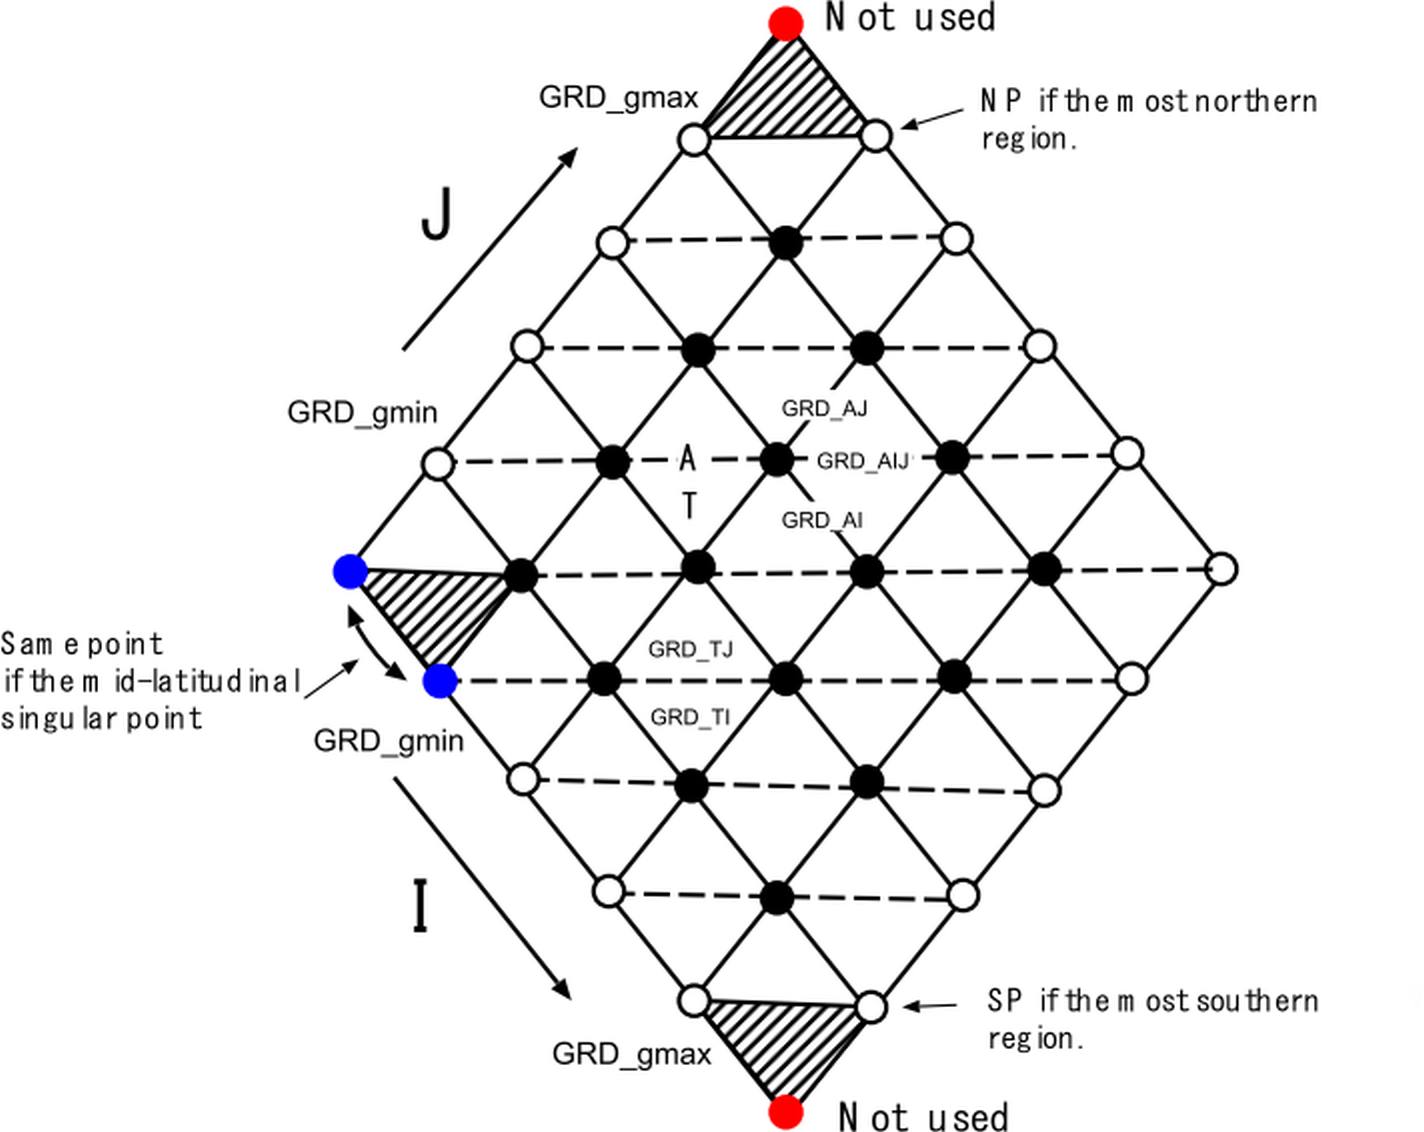
\includegraphics[scale=.5]{figs/Tomita2-12-0.png}
\caption{Schematic figure of data storing (regular region).}%
\label{f:data_store_regular}
\end{figure}



\begin{table}[htbp]
\centering
\caption{Data array for the regular region.}%
\label{t:data_array_regular}
\begin{tabular}{llll}
\hline\hline
 \multicolumn{4}{l}{\src{var(g,k,l)} : Grid point variables}\\
\hline
 $g$ & $=$ & $1 \ldots $ \text{\src{ADM_gall}} & horizontal index \\
 $k$ & $=$ & $1 \ldots $ \text{\src{ADM_kall}} & vertical index \\
 $l$ & $=$ & $1 \ldots $ \text{\src{ADM_lall}} & region index \\
\hline
 \multicolumn{4}{l}{\src{var(g,k,l,m)} : Triangle point variables}\\
\hline
 $g$ & $=$ & $1 \ldots $ \text{\src{ADM_gall}} & horizontal index \\
 $k$ & $=$ & $1 \ldots $ \text{\src{ADM_kall}} & vertical index \\
 $l$ & $=$ & $1 \ldots $ \text{\src{ADM_lall}} & region index \\
 $m$ & $=$ & \src{ADM_TI, ADM_TJ} & index of triangle position \\
\hline
 \multicolumn{4}{l}{\src{var(g,k,l,m)} : Arc point variables}\\
\hline
 $g$ & $=$ & $1 \ldots $ \text{\src{ADM_gall}} & first horizontal index \\
 $k$ & $=$ & $1 \ldots $ \text{\src{ADM_kall}} & vertical index \\
 $l$ & $=$ & $1 \ldots $ \text{\src{ADM_lall}} & region index \\
 $m$ & $=$ & \src{ADM_AI, ADM_AIJ, ADM_AJ} & index of arc position \\
\hline\hline
\end{tabular}
\end{table}


\subsection{Data array for pole region}

For pole region, \autoref{f:data_store_pole} shows the schematic figure
of data storing.
%
Only one grid point, the pole point, is managed, and the other point
marked by the white circles are the halo points, these are used only for
the reference and their values are provided from the neighboring regions
by the MPI communication or memory copy.
%
The indices for these halo are in order of clockwise direction.
%
The first dimension is horizontal suffix, and the size \src{ADM_GALL_PL} is set to 6,
one for pole point and five for halo points.
%
The second dimension is vertical suffix, which is the same with the
regular region.
%
The third dimension is region, suffix, and the range is 1 to
\src{ADM_LALL_PL}, which is the number of pole regions, and set to 2
(North pole and South pole).

Different from the regular region, the number of triangle points and arc
points are the same with the halo points, these are no need for more
dimension, and stored as the same dimensions with the grid points.
But the range of index are from \src{ADM_GMIN_PL}(=2) to \src{ADM_GMAX_PL}(=6).




\begin{figure}[htbp]
 \centering
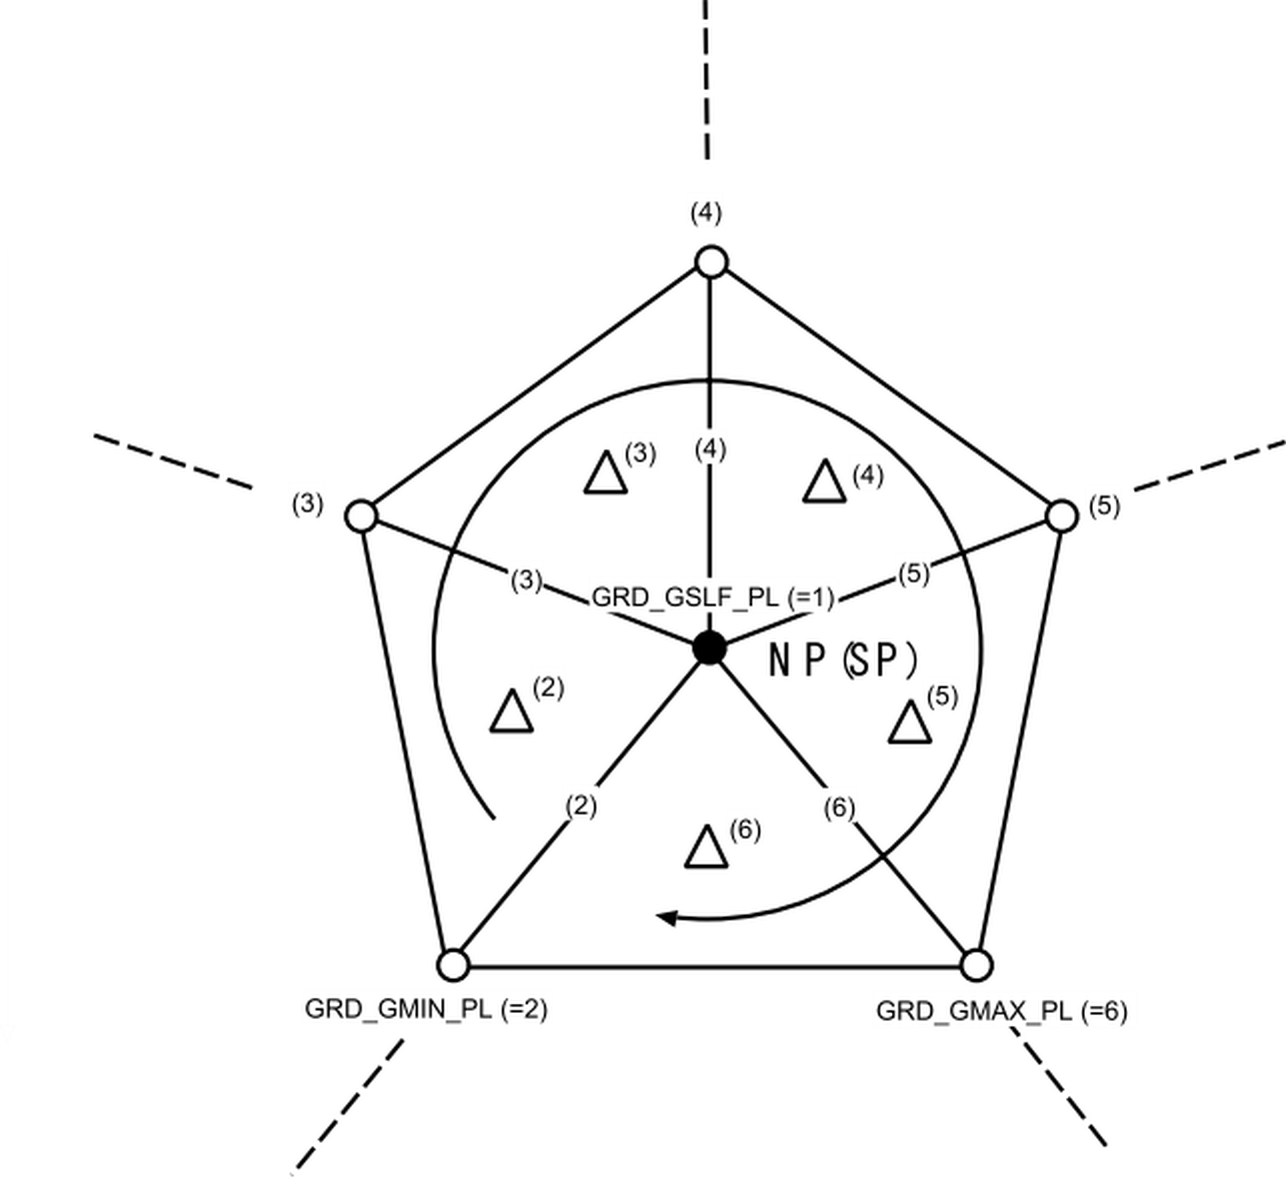
\includegraphics[scale=.5]{figs/Tomita2-12-1.png}
\caption{Schematic figure of data storing (pole region).}
\label{f:data_store_pole}
\end{figure}


\begin{table}[htbp]
\centering
\caption{Data array for the pole region.}
\begin{tabular}{llll}
\hline\hline
 \multicolumn{4}{l}{\src{var_pl(n,k,l)} : Grid, triangle, arc point variables}\\
\hline
 $n$ & $=$ & $1 \ldots $ \text{\src{ADM_GALL_PL}} & horizontal index \\
 $k$ & $=$ & $1 \ldots $ \text{\src{ADM_kall}} & vertical index \\
 $l$ & $=$ & $1 \ldots $ \text{\src{ADM_LALL_PL}} & region index \\
\hline
\end{tabular}
\end{table}

\subsection{Kernelize}

The kernels are single or multiple subroutines in original \NICAM source code,
and extracted and imposed into the wrapper for the kernel program.
%
Values of input variables in the argument list of the kernel subroutine
are stored as a data file just before the call in execution of the original \NICAM, and
they are read and given to the kernel subroutine in the kernel program.
%
Similarly values of output variables in the argument list are stored
just after the call in execution, and they are read and compared to the
actual output values of kernel subroutine, the difference are written to
the standard output for validation.

\NICAM uses several ``public object'' defined in several modules,
briefly described later.
%
Some of them are moved to \file{problem_size.inc} and \src{include}ed in
the \src{mod_misc}.



Kernel programs output several messages to the standard output, such as:
\begin{itemize}
%\setlength{\itemsep}{0pt}
 \item min/max/sum of input data,
 \item min/max/sum of output data,
 \item min/max/sum of difference between output and validation data,
 \item computational time (elapsed time).
\end{itemize}
%
Elapsed time is measured using \src{omp_get_wtime()}.

There are sample output file for the reference in \src{reference/} directory
of each kernel program, and also they are shown in``Input data and
result'' section of each kernel program in this document.

\subsection{Problem size}

In this kernel program package, problem size are set in
\file{problem_size.inc} in each kernel program, except
\src{communication}, as follows.
%
Number of grid point of one side of the region \src{ADM_gall_1d} is
$130$ including two halo points, and the total number of grid points in
whole region \src{ADM_gall} is $16900$, which corresponds to
$\text{glevel}-\text{rlevel}=7$.
%
Number of vertical layers \src{ADM_vlayer} is $40$ and the actual size
of $k$-direction \src{ADM_kall} is $42$.
%
The kernel program runs on a single process and this process manages
only one normal region, ie. \src{ADM_lall} is $1$, and also have two
pole regions, ie. \src{ADM_have_pl} is \src{.true.} and
\src{ADM_lall_pl} is $2$.
%
This normal region is to manage singular point, then
\src{ADM_have_sgp(1)} is \src{.true.}


\subsection{MPI and OpenMP}\label{s:mpi_openmpi}

While original \NICAM is parallelized by MPI and OpenMP,
all kernel program in this package except \src{communication}
are meant to be executed as one process and no threading.
%
And you don't need MPI library to compile/execute these kernel programs,
but you need to make OpneMP enable in order to use \src{omp_get_wtime()}.

\subsection{Mesuring environment}\label{s:measuring_env}

In the following sections, the example of performance result part of the
log output file of each kernel program is shown.
%
These were measured on the machine environment shown in
\autoref{t:machine_env},
with setting \src{export IAB_SYS=Ubuntu-gnu-ompi} on compilation
(See \file{QuickStart.md}).


\begin{table}[htbp]
\centering
\caption{Measuring environment}\label{t:machine_env}
\small
\begin{tabularx}{.8\textwidth}{llX}
\hline
component & specification & notes \\
\hline
 CPU & Xeon E5-2630v4 @2.2GHz (10cores) x2 & HT disabled, TB enabled\\
 Memory & 256GB &\\
 Storage & SSD (SATA) &\\
 OS & Ubuntu 16.04.4 LTS &\\
 Compiler & GNU 5.4.0 & \\
 MPI & OpenMPI 1.10.2 & Ubuntu standard \\
\hline
\end{tabularx}
\end{table}




\section{\src{dyn_diffusion}}\label{s:dyn_diffusion}

\subsection{Description}

Kernel \src{dyn_diffusion} is taken from the original subroutine
\src{OPRT_diffusion} in \NICAM.
%
This subroutine is originally defined, as you can see in that name, in module
\src{mod_oprt}.
%
This module defines several differential operators on the sphere, such
as divergence, gradient, etc.
%
Subroutine \src{OPRT_diffusion} calculates diffusion term
 of given scalar field.

\subsection{Discretization and code}


Argument lists and local variables definition part of this subroutine is
as follows.

\begin{LstF90}[name=diffusion,firstnumber=auto]
subroutine OPRT_diffusion( &
     dscl,      dscl_pl,      &
     scl,       scl_pl,       &
     kh,        kh_pl,        &
     coef_intp, coef_intp_pl, &
     coef_diff, coef_diff_pl  )
  implicit none

  real(RP), intent(out) :: dscl        (ADM_gall   ,ADM_kall,ADM_lall   )
  real(RP), intent(out) :: dscl_pl     (ADM_gall_pl,ADM_kall,ADM_lall_pl)
  real(RP), intent(in)  :: scl         (ADM_gall   ,ADM_kall,ADM_lall   )
  real(RP), intent(in)  :: scl_pl      (ADM_gall_pl,ADM_kall,ADM_lall_pl)
  real(RP), intent(in)  :: kh          (ADM_gall   ,ADM_kall,ADM_lall   )
  real(RP), intent(in)  :: kh_pl       (ADM_gall_pl,ADM_kall,ADM_lall_pl)
  real(RP), intent(in)  :: coef_intp   (ADM_gall   ,1:3,        ADM_nxyz,TI:TJ,ADM_lall   )
  real(RP), intent(in)  :: coef_intp_pl(ADM_gall_pl,1:3,        ADM_nxyz,      ADM_lall_pl)
  real(RP), intent(in)  :: coef_diff   (ADM_gall   ,1:6,        ADM_nxyz,      ADM_lall   )
  real(RP), intent(in)  :: coef_diff_pl(            1:ADM_vlink,ADM_nxyz,      ADM_lall_pl)

  real(RP) :: vt   (ADM_gall   ,ADM_nxyz,TI:TJ)
  real(RP) :: vt_pl(ADM_gall_pl,ADM_nxyz)
  real(RP) :: kf   (1:6)

  integer  :: gmin, gmax, iall, gall, kall, lall, nxyz, gminm1

  integer  :: ij
  integer  :: ip1j, ijp1, ip1jp1
  integer  :: im1j, ijm1, im1jm1

  integer  :: g, k, l, d, n, v
  !---------------------------------------------------------------------------
\end{LstF90}
%
Here \src{dscl}, \src{dscl_pl} are calculated diffusion of regular
region and polar region, respectively, from some scalar field \src{scl},
\src{scl_pl} and diffusion coefficient \src{kh}, \src{kh_pl} at the triangular points.
%
Other arguments \src{coef_intp}, \src{coef_intp_pl}, \src{coef_diff},
\src{coef_diff_pl} are various coefficients for finite difference
calculation.
%
These coefficients are calculated in advance in the subroutine
\src{OPRT_diffusion_setup}
also defined in the module (See \autoref{dyn_metrics}).
%
These are supplied as arguments, not module variables, because of the computational optimization.
The values are read from input data before executing this subroutine.

local variables
\src{vt}, \src{vt_pl} are the differentiation of given scalar field at
the gravitational center of triangles.
%
Note that the range of the last dimension is \src{TI:TJ}.
%
See below for details.
%
\src{ADM_nxyz} is \src{parameter} and the value is 3, so this dimension
shows spatial direction (X,Y,Z).


The first part of this subroutine is as follows.

\begin{LstF90}[name=diffusion,firstnumber=last]
  call DEBUG_rapstart('OPRT_diffusion')

  gmin = (ADM_gmin-1)*ADM_gall_1d + ADM_gmin
  gmax = (ADM_gmax-1)*ADM_gall_1d + ADM_gmax
  iall = ADM_gall_1d
  gall = ADM_gall
  kall = ADM_kall
  lall = ADM_lall
  nxyz = ADM_nxyz

  gminm1 = (ADM_gmin-1-1)*ADM_gall_1d + ADM_gmin-1

  !$omp parallel default(none),private(g,k,l,d,ij,ip1j,ip1jp1,ijp1,im1j,ijm1,im1jm1), &
  !$omp shared(ADM_have_sgp,gminm1,gmin,gmax,iall,gall,kall,lall,nxyz,dscl,scl,kh,kf,vt,coef_intp,coef_diff)
  do l = 1, lall
  do k = 1, kall

     do d = 1, nxyz
        !$omp do
        do g = gminm1, gmax
           ij     = g
           ip1j   = g + 1
           ip1jp1 = g + iall + 1
           ijp1   = g + iall

           vt(g,d,TI) = ( ( + 2.0_RP * coef_intp(g,1,d,TI,l) &
                            - 1.0_RP * coef_intp(g,2,d,TI,l) &
                            - 1.0_RP * coef_intp(g,3,d,TI,l) ) * scl(ij    ,k,l) &
                        + ( - 1.0_RP * coef_intp(g,1,d,TI,l) &
                            + 2.0_RP * coef_intp(g,2,d,TI,l) &
                            - 1.0_RP * coef_intp(g,3,d,TI,l) ) * scl(ip1j  ,k,l) &
                        + ( - 1.0_RP * coef_intp(g,1,d,TI,l) &
                            - 1.0_RP * coef_intp(g,2,d,TI,l) &
                            + 2.0_RP * coef_intp(g,3,d,TI,l) ) * scl(ip1jp1,k,l) &
                        ) / 3.0_RP
        enddo
        !$omp end do nowait

        !$omp do
        do g = gminm1, gmax
           ij     = g
           ip1j   = g + 1
           ip1jp1 = g + iall + 1
           ijp1   = g + iall

           vt(g,d,TJ) = ( ( + 2.0_RP * coef_intp(g,1,d,TJ,l) &
                            - 1.0_RP * coef_intp(g,2,d,TJ,l) &
                            - 1.0_RP * coef_intp(g,3,d,TJ,l) ) * scl(ij    ,k,l) &
                        + ( - 1.0_RP * coef_intp(g,1,d,TJ,l) &
                            + 2.0_RP * coef_intp(g,2,d,TJ,l) &
                            - 1.0_RP * coef_intp(g,3,d,TJ,l) ) * scl(ip1jp1,k,l) &
                        + ( - 1.0_RP * coef_intp(g,1,d,TJ,l) &
                            - 1.0_RP * coef_intp(g,2,d,TJ,l) &
                            + 2.0_RP * coef_intp(g,3,d,TJ,l) ) * scl(ijp1  ,k,l) &
                        ) / 3.0_RP
        enddo
        !$omp end do
     enddo

     if ( ADM_have_sgp(l) ) then ! pentagon
        !$omp master
        vt(gminm1,XDIR,TI) = vt(gminm1+1,XDIR,TJ)
        vt(gminm1,YDIR,TI) = vt(gminm1+1,YDIR,TJ)
        vt(gminm1,ZDIR,TI) = vt(gminm1+1,ZDIR,TJ)
        !$omp end master
     endif
\end{LstF90}

In the first part, \src{vt(:,:,TI)}, \src{vt(:,:,TJ)} are calculated
from \src{scl} with interpolation.
\autoref{f:interpolation_for_vt} shows grid arrangements.
\src{scl} are defined on white circle points in the figure,
and \src{vt} are defined on black circle points.
See \autoref{f:interpolation_for_dscl} for grid arrangement.
\src{vt} is defined on the black circle points in the figure,
while other physical quantities are defined on the white circle points.

\begin{figure}[htpb]
 \centering
 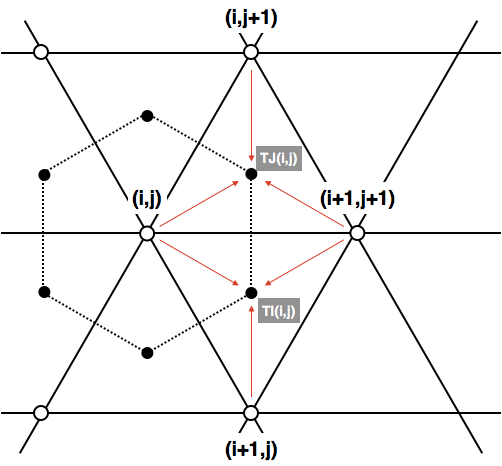
\includegraphics[scale=.4]{figs/diffusion_intp.png}
 \caption{interpolation for \src{vt}}
 \label{f:interpolation_for_vt}
\end{figure}


The second part of this subroutine is as follows.

\begin{LstF90}[name=diffusion,firstnumber=last]
!OCL XFILL
     !$omp do
     do g = 1, gmin-1
        dscl(g,k,l) = 0.0_RP
     enddo
     !$omp end do nowait

     !$omp do
     do g = gmin, gmax
        ij     = g
        ip1j   = g + 1
        ip1jp1 = g + iall + 1
        ijp1   = g + iall
        im1j   = g - 1
        im1jm1 = g - iall - 1
        ijm1   = g - iall

        kf(1) = 0.5_RP * ( kh(ij    ,k,l) + kh(ip1jp1,k,l) )
        kf(2) = 0.5_RP * ( kh(ij    ,k,l) + kh(ijp1  ,k,l) )
        kf(3) = 0.5_RP * ( kh(im1j  ,k,l) + kh(ij    ,k,l) )
        kf(4) = 0.5_RP * ( kh(im1jm1,k,l) + kh(ij    ,k,l) )
        kf(5) = 0.5_RP * ( kh(ijm1  ,k,l) + kh(ij    ,k,l) )
        kf(6) = 0.5_RP * ( kh(ij    ,k,l) + kh(ip1j  ,k,l) )

        dscl(g,k,l) = ( kf(1) * coef_diff(g,1,XDIR,l) * ( vt(ij    ,XDIR,TI) + vt(ij    ,XDIR,TJ) ) &
                      + kf(2) * coef_diff(g,2,XDIR,l) * ( vt(ij    ,XDIR,TJ) + vt(im1j  ,XDIR,TI) ) &
                      + kf(3) * coef_diff(g,3,XDIR,l) * ( vt(im1j  ,XDIR,TI) + vt(im1jm1,XDIR,TJ) ) &
                      + kf(4) * coef_diff(g,4,XDIR,l) * ( vt(im1jm1,XDIR,TJ) + vt(im1jm1,XDIR,TI) ) &
                      + kf(5) * coef_diff(g,5,XDIR,l) * ( vt(im1jm1,XDIR,TI) + vt(ijm1  ,XDIR,TJ) ) &
                      + kf(6) * coef_diff(g,6,XDIR,l) * ( vt(ijm1  ,XDIR,TJ) + vt(ij    ,XDIR,TI) ) )
     enddo
     !$omp end do

     !$omp do
     do g = gmin, gmax
        ij     = g
        ip1j   = g + 1
        ip1jp1 = g + iall + 1
        ijp1   = g + iall
        im1j   = g - 1
        im1jm1 = g - iall - 1
        ijm1   = g - iall

        kf(1) = 0.5_RP * ( kh(ij    ,k,l) + kh(ip1jp1,k,l) )
        kf(2) = 0.5_RP * ( kh(ij    ,k,l) + kh(ijp1  ,k,l) )
        kf(3) = 0.5_RP * ( kh(im1j  ,k,l) + kh(ij    ,k,l) )
        kf(4) = 0.5_RP * ( kh(im1jm1,k,l) + kh(ij    ,k,l) )
        kf(5) = 0.5_RP * ( kh(ijm1  ,k,l) + kh(ij    ,k,l) )
        kf(6) = 0.5_RP * ( kh(ij    ,k,l) + kh(ip1j  ,k,l) )

        dscl(g,k,l) = dscl(g,k,l) + ( kf(1) * coef_diff(g,1,YDIR,l) * ( vt(ij    ,XDIR,TI) + vt(ij    ,YDIR,TJ) ) &
                                    + kf(2) * coef_diff(g,2,YDIR,l) * ( vt(ij    ,XDIR,TJ) + vt(im1j  ,YDIR,TI) ) &
                                    + kf(3) * coef_diff(g,3,YDIR,l) * ( vt(im1j  ,XDIR,TI) + vt(im1jm1,YDIR,TJ) ) &
                                    + kf(4) * coef_diff(g,4,YDIR,l) * ( vt(im1jm1,XDIR,TJ) + vt(im1jm1,YDIR,TI) ) &
                                    + kf(5) * coef_diff(g,5,YDIR,l) * ( vt(im1jm1,XDIR,TI) + vt(ijm1  ,YDIR,TJ) ) &
                                    + kf(6) * coef_diff(g,6,YDIR,l) * ( vt(ijm1  ,XDIR,TJ) + vt(ij    ,YDIR,TI) ) )
     enddo
     !$omp end do

     !$omp do
     do g = gmin, gmax
        ij     = g
        ip1j   = g + 1
        ip1jp1 = g + iall + 1
        ijp1   = g + iall
        im1j   = g - 1
        im1jm1 = g - iall - 1
        ijm1   = g - iall

        kf(1) = 0.5_RP * ( kh(ij    ,k,l) + kh(ip1jp1,k,l) )
        kf(2) = 0.5_RP * ( kh(ij    ,k,l) + kh(ijp1  ,k,l) )
        kf(3) = 0.5_RP * ( kh(im1j  ,k,l) + kh(ij    ,k,l) )
        kf(4) = 0.5_RP * ( kh(im1jm1,k,l) + kh(ij    ,k,l) )
        kf(5) = 0.5_RP * ( kh(ijm1  ,k,l) + kh(ij    ,k,l) )
        kf(6) = 0.5_RP * ( kh(ij    ,k,l) + kh(ip1j  ,k,l) )

        dscl(g,k,l) = dscl(g,k,l) + ( kf(1) * coef_diff(g,1,ZDIR,l) * ( vt(ij    ,XDIR,TI) + vt(ij    ,ZDIR,TJ) ) &
                                    + kf(2) * coef_diff(g,2,ZDIR,l) * ( vt(ij    ,XDIR,TJ) + vt(im1j  ,ZDIR,TI) ) &
                                    + kf(3) * coef_diff(g,3,ZDIR,l) * ( vt(im1j  ,XDIR,TI) + vt(im1jm1,ZDIR,TJ) ) &
                                    + kf(4) * coef_diff(g,4,ZDIR,l) * ( vt(im1jm1,XDIR,TJ) + vt(im1jm1,ZDIR,TI) ) &
                                    + kf(5) * coef_diff(g,5,ZDIR,l) * ( vt(im1jm1,XDIR,TI) + vt(ijm1  ,ZDIR,TJ) ) &
                                    + kf(6) * coef_diff(g,6,ZDIR,l) * ( vt(ijm1  ,XDIR,TJ) + vt(ij    ,ZDIR,TI) ) )
     enddo
     !$omp end do nowait

!OCL XFILL
     !$omp do
     do g = gmax+1, gall
        dscl(g,k,l) = 0.0_RP
     enddo
     !$omp end do
  enddo ! loop k
  enddo ! loop l
  !$omp end parallel

\end{LstF90}


In this part, objective variable \src{dscl} is calculated
by interpolation of \src{vt}.
\autoref{f:interpolation_for_dscl} shows the grid arrangements.
\src{vt} are defined on black circle points
as \autoref{f:interpolation_for_vt},
and \src{dscl} are defined on grey diamond points.

There are three similar do-loops, each of them calculates the
contribution from X, Y, Z direction, respectively. Note that the third
dimension of \src{coef_diff} in the loop.


\begin{figure}[htbp]
\centering
 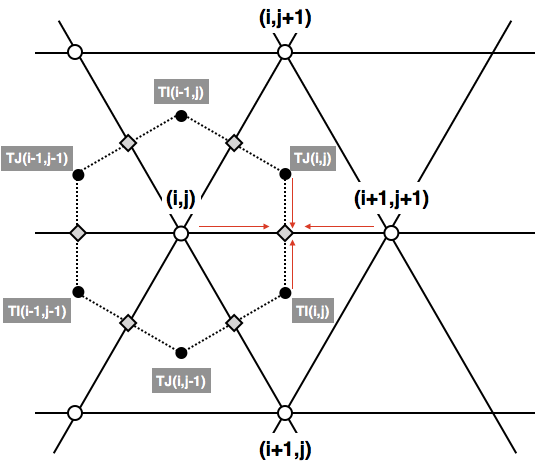
\includegraphics[scale=.4]{figs/diffusion_diff.png}
 \caption{Interpolation for \src{dscl}}\label{f:interpolation_for_dscl}
\end{figure}


The last part of this subroutine is as follows.


\begin{LstF90}[name=diffusion,firstnumber=last]
  if ( ADM_have_pl ) then
     n = ADM_gslf_pl

     do l = 1, ADM_lall_pl
     do k = 1, ADM_kall

        do d = 1, ADM_nxyz
           do v = ADM_gmin_pl, ADM_gmax_pl
              ij   = v
              ijp1 = v + 1
              if( ijp1 == ADM_gmax_pl+1 ) ijp1 = ADM_gmin_pl

              vt_pl(ij,d) = ( ( + 2.0_RP * coef_intp_pl(v,1,d,l) &
                                - 1.0_RP * coef_intp_pl(v,2,d,l) &
                                - 1.0_RP * coef_intp_pl(v,3,d,l) ) * scl_pl(n   ,k,l) &
                            + ( - 1.0_RP * coef_intp_pl(v,1,d,l) &
                                + 2.0_RP * coef_intp_pl(v,2,d,l) &
                                - 1.0_RP * coef_intp_pl(v,3,d,l) ) * scl_pl(ij  ,k,l) &
                            + ( - 1.0_RP * coef_intp_pl(v,1,d,l) &
                                - 1.0_RP * coef_intp_pl(v,2,d,l) &
                                + 2.0_RP * coef_intp_pl(v,3,d,l) ) * scl_pl(ijp1,k,l) &
                            ) / 3.0_RP
           enddo
        enddo

        dscl_pl(:,k,l) = 0.0_RP

        do v = ADM_gmin_pl, ADM_gmax_pl
           ij   = v
           ijm1 = v - 1
           if( ijm1 == ADM_gmin_pl-1 ) ijm1 = ADM_gmax_pl ! cyclic condition

           dscl_pl(n,k,l) = dscl_pl(n,k,l) &
                          + ( coef_diff_pl(v-1,XDIR,l) * ( vt_pl(ijm1,XDIR) + vt_pl(ij,XDIR) ) &
                            + coef_diff_pl(v-1,YDIR,l) * ( vt_pl(ijm1,YDIR) + vt_pl(ij,YDIR) ) &
                            + coef_diff_pl(v-1,ZDIR,l) * ( vt_pl(ijm1,ZDIR) + vt_pl(ij,ZDIR) ) &
                            ) * 0.5_RP * ( kh_pl(n,k,l) + kh_pl(ij,k,l) )
        enddo

     enddo
     enddo
  else
     dscl_pl(:,:,:) = 0.0_RP
  endif

  call DEBUG_rapend('OPRT_diffusion')

  return
end subroutine OPRT_diffusion
\end{LstF90}

The last part is for calculation for the pole region.
Variable \src{ADM_have_pl} is \src{.true.} if this process manages pole
region in original \NICAM.
For the kernel program, also set as \src{.true.} in \file{problem_size.inc}.



\subsection{Input data and result}

Max/min/sum of input/output data of the kernel subroutine are output as
a log.
%
Below is an example of \src{$IAB_SYS=Ubuntu-gnu-ompi} case.


\begin{LstLog}
 ### Input ###
 +check[check_dscl      ] max=  6.1941315670898286E-08,min= -7.0374144752795210E-08,sum= -2.7407850230958588E-07
 +check[check_dscl_pl   ] max=  2.2139244811324830E-08,min= -6.0170678327656930E-11,sum=  1.8274579608905828E-07
 +check[scl             ] max=  1.6578626530298903E-11,min= -1.2670212860993856E-11,sum= -2.0289014286353776E-10
 +check[scl_pl          ] max=  1.9358849576453664E-11,min= -8.2853331106472899E-12,sum=  1.1445754720677440E-09
 +check[kh              ] max=  2.8341305529772246E+12,min=  6.7659597088284981E+10,sum=  6.0439053980501018E+17
 +check[kh_pl           ] max=  2.8334094314435532E+12,min=  6.7659597088284981E+10,sum=  4.3486317454839525E+14
 ### Output ###
 +check[dscl            ] max=  6.1941315670898286E-08,min= -7.0374144752795210E-08,sum= -2.7407850230958588E-07
 +check[dscl_pl         ] max=  2.2139244811324830E-08,min= -6.0170678327656930E-11,sum=  1.8274579608905828E-07
 ### Validation : grid-by-grid diff ###
 +check[check_dscl      ] max=  0.0000000000000000E+00,min=  0.0000000000000000E+00,sum=  0.0000000000000000E+00
 +check[check_dscl_pl   ] max=  0.0000000000000000E+00,min=  0.0000000000000000E+00,sum=  0.0000000000000000E+00
 *** Finish kernel
\end{LstLog}

Check the lines below \src{``Validation : grid-by-grid diff''} line,
that shows difference between calculated output array and
pre-calculated reference array.
These should be zero or enough small to be acceptable.

There are sample output log files in \file{reference/}
in each kernel program directory, for reference purpose.


\subsection{Sample of perfomance result}

Here's an example of the performance result part of the log output.
Below is an example executed with the machine environment described in \autoref{s:measuring_env}.
%
Note that in this program kernel part is iterated one time.

\begin{LstLog}
 *** Computational Time Report
 *** ID=001 : MAIN_dyn_diffusion               T=     0.028 N=      1
 *** ID=002 : OPRT_diffusion                   T=     0.028 N=      1
\end{LstLog}


\section{\src{dyn_divdamp}}

\subsection{Description}

Kernel \src{dyn_divdamp} is taken from the original subroutine
\src{OPRT3D_divdamp} in \NICAM.
%
This subroutine is originally defined, as you can see in that name, in
\src{mod_oprt3d}.
%
Subroutine \src{OPRT3D_divdamp} calculates the gradient of divergence of
the vector $\{v_x, v_y, v_z\}$.
%
If this vector represents the velocity vector, this term is called
``divergence damping term''.


\subsection{Discretization and code}

Argument lists and local variables definition part of this subroutine is
as follows.

\begin{LstF90}[name=divdamp]
subroutine OPRT3D_divdamp( &
     ddivdx,    ddivdx_pl,    &
     ddivdy,    ddivdy_pl,    &
     ddivdz,    ddivdz_pl,    &
     rhogvx,    rhogvx_pl,    &
     rhogvy,    rhogvy_pl,    &
     rhogvz,    rhogvz_pl,    &
     rhogw,     rhogw_pl,     &
     coef_intp, coef_intp_pl, &
     coef_diff, coef_diff_pl  )
  implicit none

  real(RP), intent(out) :: ddivdx      (ADM_gall   ,ADM_kall,ADM_lall   ) ! tendency
  real(RP), intent(out) :: ddivdx_pl   (ADM_gall_pl,ADM_kall,ADM_lall_pl)
  real(RP), intent(out) :: ddivdy      (ADM_gall   ,ADM_kall,ADM_lall   )
  real(RP), intent(out) :: ddivdy_pl   (ADM_gall_pl,ADM_kall,ADM_lall_pl)
  real(RP), intent(out) :: ddivdz      (ADM_gall   ,ADM_kall,ADM_lall   )
  real(RP), intent(out) :: ddivdz_pl   (ADM_gall_pl,ADM_kall,ADM_lall_pl)
  real(RP), intent(in)  :: rhogvx      (ADM_gall   ,ADM_kall,ADM_lall   ) ! rho*vx { gam2 x G^1/2 }
  real(RP), intent(in)  :: rhogvx_pl   (ADM_gall_pl,ADM_kall,ADM_lall_pl)
  real(RP), intent(in)  :: rhogvy      (ADM_gall   ,ADM_kall,ADM_lall   ) ! rho*vy { gam2 x G^1/2 }
  real(RP), intent(in)  :: rhogvy_pl   (ADM_gall_pl,ADM_kall,ADM_lall_pl)
  real(RP), intent(in)  :: rhogvz      (ADM_gall   ,ADM_kall,ADM_lall   ) ! rho*vz { gam2 x G^1/2 }
  real(RP), intent(in)  :: rhogvz_pl   (ADM_gall_pl,ADM_kall,ADM_lall_pl)
  real(RP), intent(in)  :: rhogw       (ADM_gall   ,ADM_kall,ADM_lall   ) ! rho*w  { gam2 x G^1/2 }
  real(RP), intent(in)  :: rhogw_pl    (ADM_gall_pl,ADM_kall,ADM_lall_pl)
  real(RP), intent(in)  :: coef_intp   (ADM_gall   ,1:3,ADM_nxyz,TI:TJ,ADM_lall   )
  real(RP), intent(in)  :: coef_intp_pl(ADM_gall_pl,1:3,ADM_nxyz,      ADM_lall_pl)
  real(RP), intent(in)  :: coef_diff   (ADM_gall,1:6        ,ADM_nxyz,ADM_lall   )
  real(RP), intent(in)  :: coef_diff_pl(         1:ADM_vlink,ADM_nxyz,ADM_lall_pl)

  real(RP) :: sclt   (ADM_gall   ,TI:TJ) ! scalar on the hexagon vertex
  real(RP) :: sclt_pl(ADM_gall_pl)
  real(RP) :: sclt_rhogw
  real(RP) :: sclt_rhogw_pl

  real(RP) :: rhogvx_vm   (ADM_gall   )                      ! rho*vx / vertical metrics
  real(RP) :: rhogvx_vm_pl(ADM_gall_pl)
  real(RP) :: rhogvy_vm   (ADM_gall   )                      ! rho*vy / vertical metrics
  real(RP) :: rhogvy_vm_pl(ADM_gall_pl)
  real(RP) :: rhogvz_vm   (ADM_gall   )                      ! rho*vz / vertical metrics
  real(RP) :: rhogvz_vm_pl(ADM_gall_pl)
  real(RP) :: rhogw_vm    (ADM_gall,   ADM_kall,ADM_lall   ) ! rho*w  / vertical metrics
  real(RP) :: rhogw_vm_pl (ADM_gall_pl,ADM_kall,ADM_lall_pl)

  integer  :: gmin, gmax, iall, gall, kall, kmin, kmax, lall, gminm1

  integer  :: ij
  integer  :: ip1j, ijp1, ip1jp1
  integer  :: im1j, ijm1, im1jm1

  integer  :: g, k, l, n, v
  !---------------------------------------------------------------------------
\end{LstF90}

Here \src{ddivdx}, \src{ddivdy}, \src{ddivdz} are calculated x, y, z component
of the gradient of divergence, respectively.
%
And these with \src{_pl} are those for the pole region.
%
\src{rhogvx}, \src{rhogvy}, \src{rhogvz}, and \src{rhogw} are
$G^{1/2} \gamma^2  \times \rho v_x$,
$G^{1/2} \gamma^2  \times \rho v_y$,
$G^{1/2} \gamma^2  \times \rho v_z$, and
$G^{1/2} \gamma^2  \times \rho w$, respectively,
where $\{v_x, v_y, v_z\}$ are the wind vector of horizontal wind component in 3-D Cartesian
coordinates, $w$ is vertical wind,
and $G^{1/2}$ and $\gamma$ are the metrics comes from the
terrain-following coordinate described in \autoref{s:vert_coord}
%
Other arguments \src{coef_intp}, \src{coeff_diff} and those with
\src{_pl} are various coefficients for finite difference calculation,
the same with those in \src{dyn_diffusion}.

Local variable \src{sclt}, \src{sclt_pl} are the scalar value on the
gravitational cente of triangles, i.e. the vertices of the hexagonal control volume.
%
\src{rhogvx_vm} etc. are \src{rhogvx} divided by the vertical metrics.



The first part of this subroutine is as follows.

\begin{LstF90}[name=divdamp, firstnumber=last]
  call DEBUG_rapstart('OPRT3D_divdamp')

  gmin = (ADM_gmin-1)*ADM_gall_1d + ADM_gmin
  gmax = (ADM_gmax-1)*ADM_gall_1d + ADM_gmax
  iall = ADM_gall_1d
  gall = ADM_gall
  kall = ADM_kall
  kmin = ADM_kmin
  kmax = ADM_kmax
  lall = ADM_lall

  gminm1 = (ADM_gmin-1-1)*ADM_gall_1d + ADM_gmin-1

  !$omp parallel default(none),private(g,k,l), &
  !$omp shared(gall,kmin,kmax,lall,rhogw_vm,rhogvx,rhogvy,rhogvz,rhogw,VMTR_C2WfactGz,VMTR_RGSQRTH,VMTR_RGAMH)
  do l = 1, lall
     !$omp do
     do k = kmin+1, kmax
     do g = 1, gall
        rhogw_vm(g,k,l) = ( VMTR_C2WfactGz(g,k,1,l) * rhogvx(g,k  ,l) &
                          + VMTR_C2WfactGz(g,k,2,l) * rhogvx(g,k-1,l) &
                          + VMTR_C2WfactGz(g,k,3,l) * rhogvy(g,k  ,l) &
                          + VMTR_C2WfactGz(g,k,4,l) * rhogvy(g,k-1,l) &
                          + VMTR_C2WfactGz(g,k,5,l) * rhogvz(g,k  ,l) &
                          + VMTR_C2WfactGz(g,k,6,l) * rhogvz(g,k-1,l) &
                          ) * VMTR_RGAMH(g,k,l)                       & ! horizontal contribution
                        + rhogw(g,k,l) * VMTR_RGSQRTH(g,k,l)            ! vertical   contribution
     enddo
     enddo
     !$omp end do nowait

!OCL XFILL
     !$omp do
     do g = 1, gall
        rhogw_vm(g,kmin  ,l) = 0.0_RP
        rhogw_vm(g,kmax+1,l) = 0.0_RP
     enddo
     !$omp end do
  enddo
  !$omp end parallel

\end{LstF90}

This part calculates \src{rhogw_vm} from 3 components of $\rho \bm{v}$
and $\rho w$ (with the metrics).
The values are located at the triangluar points in horizonatal direction,
and at the half-integer levels in vertical direction.
%
Coefficients prefixed with \src{VMTR_} are defined and pre-calculated in
module \src{mod_vmtr} in original \NICAM.
%
When kernelize this subroutine, these definition are moved to
\src{mod_misc}, and read from the input data file.



Second part is pretty long as follows.

\begin{LstF90}[name=divdamp,firstnumber=last]
  !$omp parallel default(none),private(g,k,l,ij,ip1j,ip1jp1,ijp1,im1j,ijm1,im1jm1,sclt_rhogw), &
  !$omp shared(ADM_have_sgp,gminm1,gmin,gmax,gall,kmin,kmax,lall,iall,ddivdx,ddivdy,ddivdz,rhogvx,rhogvy,rhogvz, &
  !$omp        rhogvx_vm,rhogvy_vm,rhogvz_vm,rhogw_vm,sclt,coef_intp,coef_diff,GRD_rdgz,VMTR_RGAM)
  do l = 1, lall
     do k = kmin, kmax
!OCL XFILL
        !$omp do
        do g = 1, gall
           rhogvx_vm(g) = rhogvx(g,k,l) * VMTR_RGAM(g,k,l)
           rhogvy_vm(g) = rhogvy(g,k,l) * VMTR_RGAM(g,k,l)
           rhogvz_vm(g) = rhogvz(g,k,l) * VMTR_RGAM(g,k,l)
        enddo
        !$omp end do

        !$omp do
        do g = gminm1, gmax
           ij     = g
           ip1j   = g + 1
           ip1jp1 = g + iall + 1
           ijp1   = g + iall

           sclt_rhogw = ( ( rhogw_vm(ij,k+1,l) + rhogw_vm(ip1j,k+1,l) + rhogw_vm(ip1jp1,k+1,l) ) &
                        - ( rhogw_vm(ij,k  ,l) + rhogw_vm(ip1j,k  ,l) + rhogw_vm(ip1jp1,k  ,l) ) &
                        ) / 3.0_RP * GRD_rdgz(k)

           sclt(g,TI) = coef_intp(g,1,XDIR,TI,l) * rhogvx_vm(ij    ) &
                      + coef_intp(g,2,XDIR,TI,l) * rhogvx_vm(ip1j  ) &
                      + coef_intp(g,3,XDIR,TI,l) * rhogvx_vm(ip1jp1) &
                      + coef_intp(g,1,YDIR,TI,l) * rhogvy_vm(ij    ) &
                      + coef_intp(g,2,YDIR,TI,l) * rhogvy_vm(ip1j  ) &
                      + coef_intp(g,3,YDIR,TI,l) * rhogvy_vm(ip1jp1) &
                      + coef_intp(g,1,ZDIR,TI,l) * rhogvz_vm(ij    ) &
                      + coef_intp(g,2,ZDIR,TI,l) * rhogvz_vm(ip1j  ) &
                      + coef_intp(g,3,ZDIR,TI,l) * rhogvz_vm(ip1jp1) &
                      + sclt_rhogw
        enddo
        !$omp end do nowait

        !$omp do
        do g = gminm1, gmax
           ij     = g
           ip1j   = g + 1
           ip1jp1 = g + iall + 1
           ijp1   = g + iall

           sclt_rhogw = ( ( rhogw_vm(ij,k+1,l) + rhogw_vm(ip1jp1,k+1,l) + rhogw_vm(ijp1,k+1,l) ) &
                        - ( rhogw_vm(ij,k  ,l) + rhogw_vm(ip1jp1,k  ,l) + rhogw_vm(ijp1,k  ,l) ) &
                        ) / 3.0_RP * GRD_rdgz(k)

           sclt(g,TJ) = coef_intp(g,1,XDIR,TJ,l) * rhogvx_vm(ij    ) &
                      + coef_intp(g,2,XDIR,TJ,l) * rhogvx_vm(ip1jp1) &
                      + coef_intp(g,3,XDIR,TJ,l) * rhogvx_vm(ijp1  ) &
                      + coef_intp(g,1,YDIR,TJ,l) * rhogvy_vm(ij    ) &
                      + coef_intp(g,2,YDIR,TJ,l) * rhogvy_vm(ip1jp1) &
                      + coef_intp(g,3,YDIR,TJ,l) * rhogvy_vm(ijp1  ) &
                      + coef_intp(g,1,ZDIR,TJ,l) * rhogvz_vm(ij    ) &
                      + coef_intp(g,2,ZDIR,TJ,l) * rhogvz_vm(ip1jp1) &
                      + coef_intp(g,3,ZDIR,TJ,l) * rhogvz_vm(ijp1  ) &
                      + sclt_rhogw
        enddo
        !$omp end do

        if ( ADM_have_sgp(l) ) then ! pentagon
           !$omp master
           sclt(gminm1,TI) = sclt(gminm1+1,TJ)
           !$omp end master
        endif

!OCL XFILL
        !$omp do
        do g = 1, gmin-1
           ddivdx(g,k,l) = 0.0_RP
           ddivdy(g,k,l) = 0.0_RP
           ddivdz(g,k,l) = 0.0_RP
        enddo
        !$omp end do nowait

        !$omp do
        do g = gmin, gmax
           ij     = g
           im1j   = g - 1
           im1jm1 = g - iall - 1
           ijm1   = g - iall

           ddivdx(g,k,l) = ( coef_diff(g,1,XDIR,l) * ( sclt(ij,    TI) + sclt(ij,    TJ) ) &
                           + coef_diff(g,2,XDIR,l) * ( sclt(ij,    TJ) + sclt(im1j,  TI) ) &
                           + coef_diff(g,3,XDIR,l) * ( sclt(im1j,  TI) + sclt(im1jm1,TJ) ) &
                           + coef_diff(g,4,XDIR,l) * ( sclt(im1jm1,TJ) + sclt(im1jm1,TI) ) &
                           + coef_diff(g,5,XDIR,l) * ( sclt(im1jm1,TI) + sclt(ijm1  ,TJ) ) &
                           + coef_diff(g,6,XDIR,l) * ( sclt(ijm1,  TJ) + sclt(ij,    TI) ) )
        enddo
        !$omp end do nowait

        !$omp do
        do g = gmin, gmax
           ij     = g
           im1j   = g - 1
           im1jm1 = g - iall - 1
           ijm1   = g - iall

           ddivdy(g,k,l) = ( coef_diff(g,1,YDIR,l) * ( sclt(ij,    TI) + sclt(ij,    TJ) ) &
                           + coef_diff(g,2,YDIR,l) * ( sclt(ij,    TJ) + sclt(im1j,  TI) ) &
                           + coef_diff(g,3,YDIR,l) * ( sclt(im1j,  TI) + sclt(im1jm1,TJ) ) &
                           + coef_diff(g,4,YDIR,l) * ( sclt(im1jm1,TJ) + sclt(im1jm1,TI) ) &
                           + coef_diff(g,5,YDIR,l) * ( sclt(im1jm1,TI) + sclt(ijm1  ,TJ) ) &
                           + coef_diff(g,6,YDIR,l) * ( sclt(ijm1,  TJ) + sclt(ij,    TI) ) )
        enddo
        !$omp end do nowait

        !$omp do
        do g = gmin, gmax
           ij     = g
           im1j   = g - 1
           im1jm1 = g - iall - 1
           ijm1   = g - iall

           ddivdz(g,k,l) = ( coef_diff(g,1,ZDIR,l) * ( sclt(ij,    TI) + sclt(ij,    TJ) ) &
                           + coef_diff(g,2,ZDIR,l) * ( sclt(ij,    TJ) + sclt(im1j,  TI) ) &
                           + coef_diff(g,3,ZDIR,l) * ( sclt(im1j,  TI) + sclt(im1jm1,TJ) ) &
                           + coef_diff(g,4,ZDIR,l) * ( sclt(im1jm1,TJ) + sclt(im1jm1,TI) ) &
                           + coef_diff(g,5,ZDIR,l) * ( sclt(im1jm1,TI) + sclt(ijm1  ,TJ) ) &
                           + coef_diff(g,6,ZDIR,l) * ( sclt(ijm1,  TJ) + sclt(ij,    TI) ) )
        enddo
        !$omp end do nowait

!OCL XFILL
        !$omp do
        do g = gmax+1, gall
           ddivdx(g,k,l) = 0.0_RP
           ddivdy(g,k,l) = 0.0_RP
           ddivdz(g,k,l) = 0.0_RP
        enddo
        !$omp end do
     enddo ! loop k

!OCL XFILL
     !$omp do
     do g = 1, gall
        ddivdx(g,kmin-1,l) = 0.0_RP
        ddivdy(g,kmin-1,l) = 0.0_RP
        ddivdz(g,kmin-1,l) = 0.0_RP
        ddivdx(g,kmax+1,l) = 0.0_RP
        ddivdy(g,kmax+1,l) = 0.0_RP
        ddivdz(g,kmax+1,l) = 0.0_RP
     enddo
     !$omp end do
  enddo ! loop l
  !$omp end parallel

\end{LstF90}

In the outer most \src{l}-loop(l.98) and \src{k}-loop(l.99),
\src{sclt} at the triangular point \src{TI}(l.120) and \src{TJ}(l.144)
are calculated separately by interpolation.
%
and finally,
in the \src{g}-loop begins at l.173,
desired \src{ddivdx}(l.179), \src{ddivdy}(l.195), and
\src{ddivdz}(l.211) are calculated.


The final part is for the pole region, doing almost the same thing
as the normal region described above.

\begin{LstF90}[name=divdamp,firstnumber=last]
  if ( ADM_have_pl ) then
     n = ADM_gslf_pl

     do l = 1, ADM_lall_pl
        do k = ADM_kmin+1, ADM_kmax
        do g = 1, ADM_gall_pl
           rhogw_vm_pl(g,k,l) = ( VMTR_C2WfactGz_pl(g,k,1,l) * rhogvx_pl(g,k  ,l) &
                                + VMTR_C2WfactGz_pl(g,k,2,l) * rhogvx_pl(g,k-1,l) &
                                + VMTR_C2WfactGz_pl(g,k,3,l) * rhogvy_pl(g,k  ,l) &
                                + VMTR_C2WfactGz_pl(g,k,4,l) * rhogvy_pl(g,k-1,l) &
                                + VMTR_C2WfactGz_pl(g,k,5,l) * rhogvz_pl(g,k  ,l) &
                                + VMTR_C2WfactGz_pl(g,k,6,l) * rhogvz_pl(g,k-1,l) &
                                ) * VMTR_RGAMH_pl(g,k,l)                          & ! horizontal contribution
                              + rhogw_pl(g,k,l) * VMTR_RGSQRTH_pl(g,k,l)            ! vertical   contribution
        enddo
        enddo

        do g = 1, ADM_gall_pl
           rhogw_vm_pl(g,ADM_kmin  ,l) = 0.0_RP
           rhogw_vm_pl(g,ADM_kmax+1,l) = 0.0_RP
        enddo
     enddo

     do l = 1, ADM_lall_pl
        do k = ADM_kmin, ADM_kmax
           do v = 1, ADM_gall_pl
              rhogvx_vm_pl(v) = rhogvx_pl(v,k,l) * VMTR_RGAM_pl(v,k,l)
              rhogvy_vm_pl(v) = rhogvy_pl(v,k,l) * VMTR_RGAM_pl(v,k,l)
              rhogvz_vm_pl(v) = rhogvz_pl(v,k,l) * VMTR_RGAM_pl(v,k,l)
           enddo

           do v = ADM_gmin_pl, ADM_gmax_pl
              ij   = v
              ijp1 = v + 1
              if( ijp1 == ADM_gmax_pl+1 ) ijp1 = ADM_gmin_pl

              sclt_rhogw_pl = ( ( rhogw_vm_pl(n,k+1,l) + rhogw_vm_pl(ij,k+1,l) + rhogw_vm_pl(ijp1,k+1,l) ) &
                              - ( rhogw_vm_pl(n,k  ,l) + rhogw_vm_pl(ij,k  ,l) + rhogw_vm_pl(ijp1,k  ,l) ) &
                              ) / 3.0_RP * GRD_rdgz(k)

              sclt_pl(ij) = coef_intp_pl(v,1,XDIR,l) * rhogvx_vm_pl(n   ) &
                          + coef_intp_pl(v,2,XDIR,l) * rhogvx_vm_pl(ij  ) &
                          + coef_intp_pl(v,3,XDIR,l) * rhogvx_vm_pl(ijp1) &
                          + coef_intp_pl(v,1,YDIR,l) * rhogvy_vm_pl(n   ) &
                          + coef_intp_pl(v,2,YDIR,l) * rhogvy_vm_pl(ij  ) &
                          + coef_intp_pl(v,3,YDIR,l) * rhogvy_vm_pl(ijp1) &
                          + coef_intp_pl(v,1,ZDIR,l) * rhogvz_vm_pl(n   ) &
                          + coef_intp_pl(v,2,ZDIR,l) * rhogvz_vm_pl(ij  ) &
                          + coef_intp_pl(v,3,ZDIR,l) * rhogvz_vm_pl(ijp1) &
                          + sclt_rhogw_pl
           enddo

           ddivdx_pl(:,k,l) = 0.0_RP
           ddivdy_pl(:,k,l) = 0.0_RP
           ddivdz_pl(:,k,l) = 0.0_RP

           do v = ADM_gmin_pl, ADM_gmax_pl
              ij   = v
              ijm1 = v - 1
              if( ijm1 == ADM_gmin_pl-1 ) ijm1 = ADM_gmax_pl ! cyclic condition

              ddivdx_pl(n,k,l) = ddivdx_pl(n,k,l) + coef_diff_pl(v-1,XDIR,l) * ( sclt_pl(ijm1) + sclt_pl(ij) )
              ddivdy_pl(n,k,l) = ddivdy_pl(n,k,l) + coef_diff_pl(v-1,YDIR,l) * ( sclt_pl(ijm1) + sclt_pl(ij) )
              ddivdz_pl(n,k,l) = ddivdz_pl(n,k,l) + coef_diff_pl(v-1,ZDIR,l) * ( sclt_pl(ijm1) + sclt_pl(ij) )
           enddo
        enddo

        ddivdx_pl(:,ADM_kmin-1,l) = 0.0_RP
        ddivdx_pl(:,ADM_kmax+1,l) = 0.0_RP
        ddivdy_pl(:,ADM_kmin-1,l) = 0.0_RP
        ddivdy_pl(:,ADM_kmax+1,l) = 0.0_RP
        ddivdz_pl(:,ADM_kmin-1,l) = 0.0_RP
        ddivdz_pl(:,ADM_kmax+1,l) = 0.0_RP
     enddo
  else
     ddivdx_pl(:,:,:) = 0.0_RP
     ddivdy_pl(:,:,:) = 0.0_RP
     ddivdz_pl(:,:,:) = 0.0_RP
  endif

  call DEBUG_rapend('OPRT3D_divdamp')

  return
end subroutine OPRT3D_divdamp
\end{LstF90}




\subsection{Input data and result}

Max/min/sum of input/output data of the kernel subroutine are output as
a log.
%
Below is an example of \src{$IAB_SYS=Ubuntu-gnu-ompi} case.

\begin{LstLog}
 ### Input ###
 +check[check_ddivdx    ] max=  3.0131744015374420E-11,min= -5.2988229203876260E-11,sum= -1.6975403236890680E-11
 +check[check_ddivdx_pl ] max=  2.6717761683260969E-11,min= -5.3219224048058505E-11,sum=  4.8275913249408648E-11
 +check[check_ddivdy    ] max=  2.8051192990274010E-11,min= -2.3223214708700599E-11,sum= -4.5483269668124264E-11
 +check[check_ddivdy_pl ] max=  4.4686835079822753E-11,min= -4.1286060234480353E-11,sum=  6.8817604250940581E-11
 +check[check_ddivdz    ] max=  3.4380463226247279E-11,min= -1.3010875841849350E-11,sum= -7.2052908719075937E-11
 +check[check_ddivdz_pl ] max=  3.2276474319270210E-13,min= -8.5477300588035169E-14,sum=  3.9437219768394675E-12
 +check[rhogvx          ] max=  2.2205470252374623E-01,min= -2.0636880346843767E-01,sum= -1.7381945003843336E+02
 +check[rhogvx_pl       ] max=  1.4368235944041274E-01,min= -1.9062928892442133E-01,sum= -5.6937904377485706E+00
 +check[rhogvy          ] max=  2.4120815977222165E-01,min= -2.5907366818620919E-01,sum=  1.7927398128296358E+02
 +check[rhogvy_pl       ] max=  8.8938663283927272E-02,min= -9.6299249362234787E-02,sum= -9.3645167747781997E-03
 +check[rhogvz          ] max=  2.0899984486710360E-01,min= -1.9461784957198358E-01,sum=  2.9192900535497301E+02
 +check[rhogvz_pl       ] max=  1.2715227826262342E-03,min= -6.6561175383069663E-04,sum=  2.2146129568583188E-02
 +check[rhogw           ] max=  1.2675708942695349E-03,min= -4.2678569215437437E-03,sum= -2.6525715444058587E-02
 +check[rhogw_pl        ] max=  9.9481836269239257E-04,min= -4.2678569215437437E-03,sum= -8.3801034534239580E-02
 ### Output ###
 +check[ddivdx          ] max=  3.0131744015374420E-11,min= -5.2988229203876260E-11,sum= -1.6975403236890680E-11
 +check[ddivdx_pl       ] max=  2.6717761683260969E-11,min= -5.3219224048058505E-11,sum=  4.8275913249408648E-11
 +check[ddivdy          ] max=  2.8051192990274010E-11,min= -2.3223214708700599E-11,sum= -4.5483269668124264E-11
 +check[ddivdy_pl       ] max=  4.4686835079822753E-11,min= -4.1286060234480353E-11,sum=  6.8817604250940581E-11
 +check[ddivdz          ] max=  3.4380463226247279E-11,min= -1.3010875841849350E-11,sum= -7.2052908719075937E-11
 +check[ddivdz_pl       ] max=  3.2276474319270210E-13,min= -8.5477300588035169E-14,sum=  3.9437219768394675E-12
 ### Validation : point-by-point diff ###
 +check[check_ddivdx    ] max=  0.0000000000000000E+00,min=  0.0000000000000000E+00,sum=  0.0000000000000000E+00
 +check[check_ddivdx_pl ] max=  0.0000000000000000E+00,min=  0.0000000000000000E+00,sum=  0.0000000000000000E+00
 +check[check_ddivdy    ] max=  0.0000000000000000E+00,min=  0.0000000000000000E+00,sum=  0.0000000000000000E+00
 +check[check_ddivdy_pl ] max=  0.0000000000000000E+00,min=  0.0000000000000000E+00,sum=  0.0000000000000000E+00
 +check[check_ddivdz    ] max=  0.0000000000000000E+00,min=  0.0000000000000000E+00,sum=  0.0000000000000000E+00
 +check[check_ddivdz_pl ] max=  0.0000000000000000E+00,min=  0.0000000000000000E+00,sum=  0.0000000000000000E+00
 *** Finish kernel
\end{LstLog}

Check the lines below \src{``Validation : point-by-point diff''} line,
that shows difference between calculated output array and
pre-calculated reference array.
These should be zero or enough small to be acceptable.

There are sample output log files in \file{reference/}
in each kernel program directory, for reference purpose.


\subsection{Sample of perfomance result}


Here's an example of the performance result part of the log output.
Below is an example executed with the machine environment described in \autoref{s:measuring_env}.
%
Note that in this program kernel part is iterated one time.

\begin{LstLog}
 *** Computational Time Report
 *** ID=001 : MAIN_dyn_divdamp                 T=     0.028 N=      1
 *** ID=002 : OPRT3D_divdamp                   T=     0.028 N=      1
\end{LstLog}


\section{\src{dyn_vi_rhow_solver}}

\subsection{Description}

Kernel \src{dyn_vi_rhow_solver} is taken from the original subroutine
\src{vi_rhow_solver} in \NICAM.
%
This subrouine is originally defined in \src{mod_vi}.
%
Subroutine \src{vi_rhow_solver} is to solve the tridiagonal matrix
equations related to the vertical implicit scheme. See
\autoref{s:vert_coord} for the detail of this calculation.


\subsection{Discretization and code}

Argument lists and local variables definition part of this subroutine is
as follows.

\begin{LstF90}[name=vi_rhow_solver]
!-----------------------------------------------------------------------------
!> Tridiagonal matrix solver
subroutine vi_rhow_solver( &
     rhogw,  rhogw_pl,  &
     rhogw0, rhogw0_pl, &
     preg0,  preg0_pl,  &
     rhog0,  rhog0_pl,  &
     Srho,   Srho_pl,   &
     Sw,     Sw_pl,     &
     Spre,   Spre_pl,   &
     dt                 )
  !$ use omp_lib
  implicit none

  real(RP), intent(inout) :: rhogw    (ADM_gall   ,ADM_kall,ADM_lall   ) ! rho*w          ( G^1/2 x gam2 ), n+1
  real(RP), intent(inout) :: rhogw_pl (ADM_gall_pl,ADM_kall,ADM_lall_pl)

  real(RP), intent(in)    :: rhogw0   (ADM_gall   ,ADM_kall,ADM_lall   ) ! rho*w          ( G^1/2 x gam2 )
  real(RP), intent(in)    :: rhogw0_pl(ADM_gall_pl,ADM_kall,ADM_lall_pl)
  real(RP), intent(in)    :: preg0    (ADM_gall   ,ADM_kall,ADM_lall   ) ! pressure prime ( G^1/2 x gam2 )
  real(RP), intent(in)    :: preg0_pl (ADM_gall_pl,ADM_kall,ADM_lall_pl)
  real(RP), intent(in)    :: rhog0    (ADM_gall   ,ADM_kall,ADM_lall   ) ! rho            ( G^1/2 x gam2 )
  real(RP), intent(in)    :: rhog0_pl (ADM_gall_pl,ADM_kall,ADM_lall_pl)
  real(RP), intent(in)    :: Srho     (ADM_gall   ,ADM_kall,ADM_lall   ) ! source term for rho  at the full level
  real(RP), intent(in)    :: Srho_pl  (ADM_gall_pl,ADM_kall,ADM_lall_pl)
  real(RP), intent(in)    :: Sw       (ADM_gall   ,ADM_kall,ADM_lall   ) ! source term for rhow at the half level
  real(RP), intent(in)    :: Sw_pl    (ADM_gall_pl,ADM_kall,ADM_lall_pl)
  real(RP), intent(in)    :: Spre     (ADM_gall   ,ADM_kall,ADM_lall   ) ! source term for pres at the full level
  real(RP), intent(in)    :: Spre_pl  (ADM_gall_pl,ADM_kall,ADM_lall_pl)
  real(RP), intent(in)    :: dt

  real(RP) :: Sall    (ADM_gall,   ADM_kall)
  real(RP) :: Sall_pl (ADM_gall_pl,ADM_kall)
  real(RP) :: beta    (ADM_gall   )
  real(RP) :: beta_pl (ADM_gall_pl)
  real(RP) :: gamma   (ADM_gall,   ADM_kall)
  real(RP) :: gamma_pl(ADM_gall_pl,ADM_kall)

  integer  :: gall, kmin, kmax, lall
  real(RP) :: grav
  real(RP) :: CVovRt2 ! Cv / R / dt**2
  real(RP) :: alpha

  integer  :: g, k, l
  integer  :: gstr, gend
  !$ integer  :: n_per_thread
  !$ integer  :: n_thread
  !---------------------------------------------------------------------------

\end{LstF90}

Here \src{rhogw} is $\rho \times w$ with metric $G^{1/2} \gamma^2$
multiplied at new time step $n+1$.
%
\src{rhogw0}, \src{preg0}, \src{rhog0}, are 
$\rho \times w$, pressure, $\rho$
with metric multiplied at time step $n$, respectively.
%
\src{Srho}, \src{Sw}, \src{Spre} are
source term for $\rho$ at the full level,
source term for $\rho \times w$ at the half level,
source term for pressure at the full level, respectively.
%
Other arguments with suffix \src{_pl} are for the pole region.
%
\src{dt} is a time step for fast-mode.

Among local variables,
\src{alpha} is the flag for non-hydrostatic/hydrostatic.
In this kernel, set to $1$ in \src{problem_size.inc}.




Main part of this subroutine is as follows.

\begin{LstF90}[name=vi_rhow_solver,firstnumber=last]
  call DEBUG_rapstart('____vi_rhow_solver')

  gall = ADM_gall
  kmin = ADM_kmin
  kmax = ADM_kmax
  lall = ADM_lall

  grav    = CONST_GRAV
  CVovRt2 = CONST_CVdry / CONST_Rdry / (dt*dt)
  alpha   = real(NON_HYDRO_ALPHA,kind=RP)

  !$omp parallel default(none),private(g,k,l), &
  !$omp private(gstr,gend,n_thread,n_per_thread) &
  !$omp shared(gall,kmin,kmax,lall,rhogw,rhogw0,preg0,rhog0,Srho,Sw,Spre,dt,Sall,beta,gamma,Mu,Mc,Ml, &
  !$omp        GRD_afact,GRD_bfact,GRD_rdgzh,VMTR_GSGAM2H,VMTR_RGAM,VMTR_RGAMH,VMTR_RGSGAM2,VMTR_RGSGAM2H,grav,alpha,CVovRt2)
  gstr = 1
  gend = gall
  !$ n_thread     = omp_get_num_threads()
  !$ n_per_thread = gall / n_thread + int( 0.5_RP + sign(0.5_RP,mod(gall,n_thread)-0.5_RP) )
  !$ gstr         = n_per_thread * omp_get_thread_num() + 1
  !$ gend         = min( gstr+n_per_thread-1, gall )

  do l = 1, lall
     ! calc Sall
     do k = kmin+1, kmax
     do g = gstr, gend
        Sall(g,k) = (   ( rhogw0(g,k,  l)*alpha + dt * Sw  (g,k,  l) ) * VMTR_RGAMH  (g,k,  l)**2             &
                    - ( ( preg0 (g,k,  l)       + dt * Spre(g,k,  l) ) * VMTR_RGSGAM2(g,k,  l)                &
                      - ( preg0 (g,k-1,l)       + dt * Spre(g,k-1,l) ) * VMTR_RGSGAM2(g,k-1,l)                &
                      ) * dt * GRD_rdgzh(k)                                                                   &
                    - ( ( rhog0 (g,k,  l)       + dt * Srho(g,k,  l) ) * VMTR_RGAM(g,k,  l)**2 * GRD_afact(k) &
                      + ( rhog0 (g,k-1,l)       + dt * Srho(g,k-1,l) ) * VMTR_RGAM(g,k-1,l)**2 * GRD_bfact(k) &
                      ) * dt * grav                                                                           &
                    ) * CVovRt2
     enddo
     enddo

     ! boundary conditions
     do g = gstr, gend
        rhogw(g,kmin,  l) = rhogw(g,kmin,  l) * VMTR_RGSGAM2H(g,kmin,  l)
        rhogw(g,kmax+1,l) = rhogw(g,kmax+1,l) * VMTR_RGSGAM2H(g,kmax+1,l)
        Sall (g,kmin+1)   = Sall (g,kmin+1) - Ml(g,kmin+1,l) * rhogw(g,kmin,  l)
        Sall (g,kmax  )   = Sall (g,kmax  ) - Mu(g,kmax,  l) * rhogw(g,kmax+1,l)
     enddo

     !---< solve tri-daigonal matrix >

     ! condition at kmin+1
     k = kmin+1
     do g = gstr, gend
        beta (g)     = Mc(g,k,l)
        rhogw(g,k,l) = Sall(g,k) / beta(g)
     enddo

     ! forward
     do k = kmin+2, kmax
     do g = gstr, gend
        gamma(g,k)   = Mu(g,k-1,l) / beta(g)
        beta (g)     = Mc(g,k,l) - Ml(g,k,l) * gamma(g,k) ! update beta
        rhogw(g,k,l) = ( Sall(g,k) - Ml(g,k,l) * rhogw(g,k-1,l) ) / beta(g)
     enddo
     enddo

     ! backward
     do k = kmax-1, kmin+1, -1
     do g = gstr, gend
        rhogw(g,k  ,l) = rhogw(g,k  ,l) - gamma(g,k+1) * rhogw(g,k+1,l)
        rhogw(g,k+1,l) = rhogw(g,k+1,l) * VMTR_GSGAM2H(g,k+1,l) ! return value ( G^1/2 x gam2 )
     enddo
     enddo

     ! boundary treatment
     do g = gstr, gend
        rhogw(g,kmin  ,l) = rhogw(g,kmin  ,l) * VMTR_GSGAM2H(g,kmin  ,l)
        rhogw(g,kmin+1,l) = rhogw(g,kmin+1,l) * VMTR_GSGAM2H(g,kmin+1,l)
        rhogw(g,kmax+1,l) = rhogw(g,kmax+1,l) * VMTR_GSGAM2H(g,kmax+1,l)
     enddo
  enddo
  !$omp end parallel
\end{LstF90}

Inside of the long $l$-loop(l.72), the first $k$-loop(l.73) calcurates total source
term \src{Sall}.
%
The section after setting the boundary condition at \src{kmin} and \src{kmax}
solves tri-diagonal matrix.
%
Its first part(l.97 to l.111) is for forward elimination and the second
part(l.114 to l.119) is for backward substitution.

Note that elements of the tridiagonal matrix \src{Mc}, \src{Mu} and
\src{Ml} are calculated in advance by other subroutine in the original
module, and they are read from input data file in this kernel program.


The last part of this subroutine is for the pole region, doing almost
the same process as the normal region.

\begin{LstF90}[name=vi_rhow_solver,firstnumber=last,breaklines=false]
  if ( ADM_have_pl ) then
     do l = 1, ADM_lall_pl
        do k  = ADM_kmin+1, ADM_kmax
        do g = 1, ADM_gall_pl
           Sall_pl(g,k) = (   ( rhogw0_pl(g,k,  l)*alpha + dt * Sw_pl  (g,k,  l) ) * VMTR_RGAMH_pl  (g,k,  l)**2             &
                          - ( ( preg0_pl (g,k,  l)       + dt * Spre_pl(g,k,  l) ) * VMTR_RGSGAM2_pl(g,k,  l)                &
                            - ( preg0_pl (g,k-1,l)       + dt * Spre_pl(g,k-1,l) ) * VMTR_RGSGAM2_pl(g,k-1,l)                &
                            ) * dt * GRD_rdgzh(k)                                                                            &
                          - ( ( rhog0_pl (g,k,  l)       + dt * Srho_pl(g,k,  l) ) * VMTR_RGAM_pl(g,k,  l)**2 * GRD_afact(k) &
                            + ( rhog0_pl (g,k-1,l)       + dt * Srho_pl(g,k-1,l) ) * VMTR_RGAM_pl(g,k-1,l)**2 * GRD_bfact(k) &
                            ) * dt * grav                                                                                    &
                          ) * CVovRt2
        enddo
        enddo

        do g = 1, ADM_gall_pl
           rhogw_pl(g,ADM_kmin,  l) = rhogw_pl(g,ADM_kmin,  l) * VMTR_RGSGAM2H_pl(g,ADM_kmin,  l)
           rhogw_pl(g,ADM_kmax+1,l) = rhogw_pl(g,ADM_kmax+1,l) * VMTR_RGSGAM2H_pl(g,ADM_kmax+1,l)
           Sall_pl (g,ADM_kmin+1)   = Sall_pl (g,ADM_kmin+1) - Ml_pl(g,ADM_kmin+1,l) * rhogw_pl(g,ADM_kmin,  l)
           Sall_pl (g,ADM_kmax  )   = Sall_pl (g,ADM_kmax  ) - Mu_pl(g,ADM_kmax,  l) * rhogw_pl(g,ADM_kmax+1,l)
        enddo

        k = ADM_kmin+1
        do g = 1, ADM_gall_pl
           beta_pl (g)     = Mc_pl(g,k,l)
           rhogw_pl(g,k,l) = Sall_pl(g,k) / beta_pl(g)
        enddo

        do k = ADM_kmin+2, ADM_kmax
        do g = 1, ADM_gall_pl
           gamma_pl(g,k)   = Mu_pl(g,k-1,l) / beta_pl(g)
           beta_pl (g)     = Mc_pl(g,k,l) - Ml_pl(g,k,l) * gamma_pl(g,k) ! update beta
           rhogw_pl(g,k,l) = ( Sall_pl(g,k) - Ml_pl(g,k,l) * rhogw_pl(g,k-1,l) ) / beta_pl(g)
        enddo
        enddo

        ! backward
        do k = ADM_kmax-1, ADM_kmin+1, -1
        do g = 1, ADM_gall_pl
           rhogw_pl(g,k  ,l) = rhogw_pl(g,k  ,l) - gamma_pl(g,k+1) * rhogw_pl(g,k+1,l)
           rhogw_pl(g,k+1,l) = rhogw_pl(g,k+1,l) * VMTR_GSGAM2H_pl(g,k+1,l) ! return value ( G^1/2 x gam2 )
        enddo
        enddo

        ! boundary treatment
        do g = 1, ADM_gall_pl
           rhogw_pl(g,ADM_kmin  ,l) = rhogw_pl(g,ADM_kmin  ,l) * VMTR_GSGAM2H_pl(g,ADM_kmin  ,l)
           rhogw_pl(g,ADM_kmin+1,l) = rhogw_pl(g,ADM_kmin+1,l) * VMTR_GSGAM2H_pl(g,ADM_kmin+1,l)
           rhogw_pl(g,ADM_kmax+1,l) = rhogw_pl(g,ADM_kmax+1,l) * VMTR_GSGAM2H_pl(g,ADM_kmax+1,l)
        enddo
     enddo
  endif

  call DEBUG_rapend('____vi_rhow_solver')

  return
end subroutine vi_rhow_solver
\end{LstF90}

\subsection{Input data and result}

Max/min/sum of input/output data of the kernel subroutine are output as
a log.
%
Below is an example of \src{$IAB_SYS=Ubuntu-gnu-ompi} case.


\begin{LstLog}
 ### Input ###
 +check[rhogw_prev      ] max=  1.0733675425174699E-14,min= -2.5212277839542070E-18,sum=  2.1443525022460023E-14
 +check[rhogw_prev_pl   ] max=  1.0733675425174699E-14,min= -3.0929371635479732E-15,sum=  7.6415689931329447E-15
 +check[check_rhogw     ] max=  6.3321830580406713E-01,min= -5.5759247708875415E-01,sum=  3.9071354372140144E+02
 +check[check_rhogw_pl  ] max=  9.9023353298473032E-02,min= -7.4852014128754477E-03,sum=  2.1725659627743767E+00
 +check[rhogw0          ] max=  1.2675708942695349E-03,min= -4.2678569215437437E-03,sum= -2.6525715444058587E-02
 +check[rhogw0_pl       ] max=  9.9481836269239257E-04,min= -4.2678569215437437E-03,sum= -8.3801034534239580E-02
 +check[preg0           ] max=  1.4047194007847271E+01,min= -2.6115802085359952E+01,sum= -1.0687083035942905E+05
 +check[preg0_pl        ] max=  1.3572400586711277E+01,min= -2.6115802085359952E+01,sum=  3.4640462790019097E+02
 +check[Srho            ] max=  3.3317357550311205E-04,min= -3.9691441465327759E-04,sum= -2.7468694177252501E-01
 +check[Srho_pl         ] max=  4.3441154740222974E-05,min= -2.2770470374092324E-05,sum= -3.8685936849254728E-05
 +check[Sw              ] max=  2.4651449651180712E-04,min= -3.2516247664737818E-04,sum= -1.6092196259156019E-01
 +check[Sw_pl           ] max=  2.8812604579719903E-04,min= -5.5442162236740700E-04,sum= -1.1046915056782920E-02
 +check[Spre            ] max=  3.6234075910381584E+01,min= -3.7498614557267203E+01,sum= -2.4763893276893483E+04
 +check[Spre_pl         ] max=  4.4863109100507081E+00,min= -2.0915571645010926E+00,sum=  1.0496606720811164E+00
 +check[Mc              ] max=  1.7037935104756485E+00,min=  0.0000000000000000E+00,sum=  8.2325595392291399E+05
 +check[Mc_pl           ] max=  1.4569727548844720E+00,min=  2.3177911966477871-310,sum=  6.0165678214473996E+02
 +check[Ml              ] max=  0.0000000000000000E+00,min= -8.3019108752152282E-01,sum= -3.9659607793632336E+05
 +check[Ml_pl           ] max=  3.2282782818256430E+02,min= -6.9953788050738130E-01,sum=  3.4604237063825449E+03
 +check[Mu              ] max=  0.0000000000000000E+00,min= -8.6888851023079583E-01,sum= -4.2616616191494197E+05
 +check[Mu_pl           ] max=  9.7233873292775215E+01,min= -7.5264063505825385E-01,sum=  8.5169724995286754E+02
 ### Output ###
 +check[rhogw           ] max=  6.3321830580406713E-01,min= -5.5759247708875415E-01,sum=  3.9071354372140144E+02
 +check[rhogw_pl        ] max=  9.9023353298473032E-02,min= -7.4852014128754477E-03,sum=  2.1725659627743767E+00
 ### Validation : grid-by-grid diff ###
 +check[check_rhogw     ] max=  0.0000000000000000E+00,min=  0.0000000000000000E+00,sum=  0.0000000000000000E+00
 +check[check_rhogw_pl  ] max=  0.0000000000000000E+00,min=  0.0000000000000000E+00,sum=  0.0000000000000000E+00
 *** Finish kernel
\end{LstLog}

Check the lines below \src{``Validation : grid-by-grid diff''} line,
that shows difference between calculated output array and
pre-calculated reference array.
These should be zero or enough small to be acceptable.

There are sample output log files in \file{reference/} 
in each kernel program directory, for reference purpose.



\subsection{Sample of perfomance result}

Here's an example of the performance result part of the log output.
Below is an example executed with the machine environment described in \autoref{s:measuring_env}.
%
Note that in this program kernel part is iterated one time.

\begin{LstLog}
 *** Computational Time Report
 *** ID=001 : MAIN_dyn_vi_rhow_solver          T=     0.016 N=      1
 *** ID=002 : ____vi_rhow_solver               T=     0.016 N=      1
\end{LstLog}
\section{\src{dyn_vert_adv_limiter}}
\label{dyn_vert_adv_limiter}

\subsection{Description}

Kernel \src{dyn_vert_adv_limiter} is taken from the original
subroutine \src{vertical_limiter_thuburn} in \NICAM.
%
This subroutine is originally defined in \src{mod_src_tracer}, that is
to contain several subroutines for tracer advection.
%
Subroutine \src{vertical_limiter_thuburn} is to ensure distribution of
tracer quantities' monotonicity in advection scheme, using the flux
limitter proposed by \cite{Thuburn:1996in}.
%
This subroutine is for vertical advection only and horizontal advection
is treated by other subroutine \src{horizontal_limiter_thuburn}, which
is also kernelized in this pacakage (See \autoref{dyn_horiz_adv_limiter}).
%
See section 4. in \cite{Tomita2010ecmwf} for details of the tracer scheme in \NICAM.


\subsection{Discretization and code}

Argument lists and local variables definition part of this subroutine is
as follows.

\begin{LstF90}[name=vertical_limiter_thuburn]
subroutine vertical_limiter_thuburn( &
     q_h, q_h_pl, &
     q,   q_pl,   &
     d,   d_pl,   &
     ck,  ck_pl   )
!ESC!    use mod_const, only: &
!ESC!       CONST_HUGE, &
!ESC!       CONST_EPS
!ESC!    use mod_adm, only: &
!ESC!       ADM_have_pl, &
!ESC!       ADM_gall,    &
!ESC!       ADM_gall_pl, &
!ESC!       ADM_lall,    &
!ESC!       ADM_lall_pl, &
!ESC!       ADM_kall,    &
!ESC!       ADM_kmin,    &
!ESC!       ADM_kmax
  implicit none

  real(RP), intent(inout) :: q_h   (ADM_gall   ,ADM_kall,ADM_lall   )
  real(RP), intent(inout) :: q_h_pl(ADM_gall_pl,ADM_kall,ADM_lall_pl)
  real(RP), intent(in)    :: q     (ADM_gall   ,ADM_kall,ADM_lall   )
  real(RP), intent(in)    :: q_pl  (ADM_gall_pl,ADM_kall,ADM_lall_pl)
  real(RP), intent(in)    :: d     (ADM_gall   ,ADM_kall,ADM_lall   )
  real(RP), intent(in)    :: d_pl  (ADM_gall_pl,ADM_kall,ADM_lall_pl)
  real(RP), intent(in)    :: ck    (ADM_gall   ,ADM_kall,ADM_lall   ,2)
  real(RP), intent(in)    :: ck_pl (ADM_gall_pl,ADM_kall,ADM_lall_pl,2)

  real(RP) :: Qout_min_k
  real(RP) :: Qout_max_k
  real(RP) :: Qout_min_km1(ADM_gall)
  real(RP) :: Qout_max_km1(ADM_gall)
  real(RP) :: Qout_min_pl(ADM_gall_pl,ADM_kall)
  real(RP) :: Qout_max_pl(ADM_gall_pl,ADM_kall)

  real(RP) :: Qin_minL, Qin_maxL
  real(RP) :: Qin_minU, Qin_maxU
  real(RP) :: qnext_min, qnext_max
  real(RP) :: Cin, Cout
  real(RP) :: CQin_min, CQin_max
  real(RP) :: inflagL, inflagU
  real(RP) :: zerosw

  integer  :: gall, kmin, kmax
  real(RP) :: EPS, BIG

  integer  :: g, k, l
  !---------------------------------------------------------------------------
\end{LstF90}
%
Here \src{q_h} is $q$ at half level of the vertical layer, which modified by the flux limiter.
%
\src{q} is $q$ at grid point,
\src{ck} is Courant number,
\src{d} is a correction factor derived from an artificial viscosity for the total density.
%
Note that \src{ck} has the 4th dimension whose size is 2, which specify
lower/upper face, i.e. half integer level.



The first section of the subroutine is as follows.

\begin{LstF90}[name=vertical_limiter_thuburn]
  call DEBUG_rapstart('____vertical_adv_limiter')

  gall = ADM_gall
  kmin = ADM_kmin
  kmax = ADM_kmax

  EPS  = CONST_EPS
  BIG  = CONST_HUGE

  do l = 1, ADM_lall
     !$omp parallel default(none), &
     !$omp private(g,k,zerosw,inflagL,inflagU,Qin_minL,Qin_minU,Qin_maxL,Qin_maxU, &
     !$omp         qnext_min,qnext_max,Cin,Cout,CQin_min,CQin_max,Qout_min_k,Qout_max_k),  &
     !$omp shared(l,gall,kmin,kmax,q_h,ck,q,d,Qout_min_km1,Qout_max_km1,EPS,BIG)

!OCL XFILL
       !$omp do
       do g = 1, gall
          k = kmin ! peeling

          inflagL = 0.5_RP - sign(0.5_RP,ck(g,k  ,l,1)) ! incoming flux: flag=1
          inflagU = 0.5_RP + sign(0.5_RP,ck(g,k+1,l,1)) ! incoming flux: flag=1

          Qin_minL = min( q(g,k,l), q(g,k-1,l) ) + ( 1.0_RP-inflagL ) * BIG
          Qin_minU = min( q(g,k,l), q(g,k+1,l) ) + ( 1.0_RP-inflagU ) * BIG
          Qin_maxL = max( q(g,k,l), q(g,k-1,l) ) - ( 1.0_RP-inflagL ) * BIG
          Qin_maxU = max( q(g,k,l), q(g,k+1,l) ) - ( 1.0_RP-inflagU ) * BIG

          qnext_min = min( Qin_minL, Qin_minU, q(g,k,l) )
          qnext_max = max( Qin_maxL, Qin_maxU, q(g,k,l) )

          Cin      = (        inflagL ) * ck(g,k,l,1) &
                   + (        inflagU ) * ck(g,k,l,2)
          Cout     = ( 1.0_RP-inflagL ) * ck(g,k,l,1) &
                   + ( 1.0_RP-inflagU ) * ck(g,k,l,2)

          CQin_min = (        inflagL ) * ck(g,k,l,1) * Qin_minL &
                   + (        inflagU ) * ck(g,k,l,2) * Qin_minU
          CQin_max = (        inflagL ) * ck(g,k,l,1) * Qin_maxL &
                   + (        inflagU ) * ck(g,k,l,2) * Qin_maxU

          zerosw = 0.5_RP - sign(0.5_RP,abs(Cout)-EPS) ! if Cout = 0, sw = 1

          Qout_min_k = ( ( q(g,k,l) - qnext_max ) + qnext_max*(Cin+Cout-d(g,k,l)) - CQin_max ) &
                     / ( Cout + zerosw ) * ( 1.0_RP - zerosw )                                 &
                     + q(g,k,l) * zerosw
          Qout_max_k = ( ( q(g,k,l) - qnext_min ) + qnext_min*(Cin+Cout-d(g,k,l)) - CQin_min ) &
                     / ( Cout + zerosw ) * ( 1.0_RP - zerosw )                                 &
                     + q(g,k,l) * zerosw

          Qout_min_km1(g) = Qout_min_k
          Qout_max_km1(g) = Qout_max_k
       enddo
       !$omp end do

       do k = kmin+1, kmax
!OCL XFILL
          !$omp do
          do g = 1, gall
             inflagL = 0.5_RP - sign(0.5_RP,ck(g,k  ,l,1)) ! incoming flux: flag=1
             inflagU = 0.5_RP + sign(0.5_RP,ck(g,k+1,l,1)) ! incoming flux: flag=1

             Qin_minL = min( q(g,k,l), q(g,k-1,l) ) + ( 1.0_RP-inflagL ) * BIG
             Qin_minU = min( q(g,k,l), q(g,k+1,l) ) + ( 1.0_RP-inflagU ) * BIG
             Qin_maxL = max( q(g,k,l), q(g,k-1,l) ) - ( 1.0_RP-inflagL ) * BIG
             Qin_maxU = max( q(g,k,l), q(g,k+1,l) ) - ( 1.0_RP-inflagU ) * BIG

             qnext_min = min( Qin_minL, Qin_minU, q(g,k,l) )
             qnext_max = max( Qin_maxL, Qin_maxU, q(g,k,l) )

             Cin      = (        inflagL ) * ck(g,k,l,1) &
                      + (        inflagU ) * ck(g,k,l,2)
             Cout     = ( 1.0_RP-inflagL ) * ck(g,k,l,1) &
                      + ( 1.0_RP-inflagU ) * ck(g,k,l,2)

             CQin_min = (        inflagL ) * ck(g,k,l,1) * Qin_minL &
                      + (        inflagU ) * ck(g,k,l,2) * Qin_minU
             CQin_max = (        inflagL ) * ck(g,k,l,1) * Qin_maxL &
                      + (        inflagU ) * ck(g,k,l,2) * Qin_maxU

             zerosw = 0.5_RP - sign(0.5_RP,abs(Cout)-EPS) ! if Cout = 0, sw = 1

             Qout_min_k = ( ( q(g,k,l) - qnext_max ) + qnext_max*(Cin+Cout-d(g,k,l)) - CQin_max ) &
                        / ( Cout + zerosw ) * ( 1.0_RP - zerosw )                                 &
                        + q(g,k,l) * zerosw
             Qout_max_k = ( ( q(g,k,l) - qnext_min ) + qnext_min*(Cin+Cout-d(g,k,l)) - CQin_min ) &
                        / ( Cout + zerosw ) * ( 1.0_RP - zerosw )                                 &
                        + q(g,k,l) * zerosw

             q_h(g,k,l) = (        inflagL ) * max( min( q_h(g,k,l), Qout_max_km1(g) ), Qout_min_km1(g) ) &
                        + ( 1.0_RP-inflagL ) * max( min( q_h(g,k,l), Qout_max_k      ), Qout_min_k      )

             Qout_min_km1(g) = Qout_min_k
             Qout_max_km1(g) = Qout_max_k
          enddo
          !$omp end do
       enddo

     !$omp end parallel
  enddo

\end{LstF90}
%
In the long $l$-loop, there seems to be two blocks, but they are almost
the same, except that the first one is only for \src{kmin}, that is the
lowest level, and the second one is the rest of \src{k} to the top level.
%
\src{inflagL} and \src{inflagU} are flag that takes the value $1$ if there is an
incoming flux to the current layer through the lower/upper face.
%
\src{Qin_*} are the smaller/larger values of $q$ at lower/upper
neighboring layer, that is meaningful only if inflag at lower/upper is $1$.
%
\src{Cin} and \src{Cout} are the sum of Courant number at both face of
the layer, for example, \src{Cin} is the sum of \src{ck} at lower face
and upper face, if both of \src{inflagL} and \src{inflagU} is $1$, which
means that there are inflow through both lower/upper face.
%
\src{CQin_*} are the min/max of \src{Cin} times \src{Qin_*}, which
specify the minimun/maximum of inflow.
%
Then \src{CQout_*} are calculated.
%
Finaly \src{q_h} is calculated, which is bounded by \src{Qout_*}.


The second section of this subroutine is as follows.

\begin{LstF90}[name=vertical_limiter_thuburn]
  if ( ADM_have_pl ) then
     do l = 1, ADM_lall_pl

        do k = ADM_kmin, ADM_kmax
          do g = 1, ADM_gall_pl
             inflagL = 0.5_RP - sign(0.5_RP,ck_pl(g,k  ,l,1)) ! incoming flux: flag=1
             inflagU = 0.5_RP + sign(0.5_RP,ck_pl(g,k+1,l,1)) ! incoming flux: flag=1

             Qin_minL = min( q_pl(g,k,l), q_pl(g,k-1,l) ) + ( 1.0_RP-inflagL ) * BIG
             Qin_minU = min( q_pl(g,k,l), q_pl(g,k+1,l) ) + ( 1.0_RP-inflagU ) * BIG
             Qin_maxL = max( q_pl(g,k,l), q_pl(g,k-1,l) ) - ( 1.0_RP-inflagL ) * BIG
             Qin_maxU = max( q_pl(g,k,l), q_pl(g,k+1,l) ) - ( 1.0_RP-inflagU ) * BIG

             qnext_min = min( Qin_minL, Qin_minU, q_pl(g,k,l) )
             qnext_max = max( Qin_maxL, Qin_maxU, q_pl(g,k,l) )

             Cin      = (        inflagL ) * ( ck_pl(g,k,l,1) ) &
                      + (        inflagU ) * ( ck_pl(g,k,l,2) )
             Cout     = ( 1.0_RP-inflagL ) * ( ck_pl(g,k,l,1) ) &
                      + ( 1.0_RP-inflagU ) * ( ck_pl(g,k,l,2) )

             CQin_max = (        inflagL ) * ( ck_pl(g,k,l,1) * Qin_maxL ) &
                      + (        inflagU ) * ( ck_pl(g,k,l,2) * Qin_maxU )
             CQin_min = (        inflagL ) * ( ck_pl(g,k,l,1) * Qin_minL ) &
                      + (        inflagU ) * ( ck_pl(g,k,l,2) * Qin_minU )

             zerosw = 0.5_RP - sign(0.5_RP,abs(Cout)-EPS) ! if Cout = 0, sw = 1

             Qout_min_pl(g,k) = ( ( q_pl(g,k,l) - qnext_max ) + qnext_max*(Cin+Cout-d_pl(g,k,l)) - CQin_max ) &
                              / ( Cout + zerosw ) * ( 1.0_RP - zerosw )                                       &
                              + q_pl(g,k,l) * zerosw
             Qout_max_pl(g,k) = ( ( q_pl(g,k,l) - qnext_min ) + qnext_min*(Cin+Cout-d_pl(g,k,l)) - CQin_min ) &
                              / ( Cout + zerosw ) * ( 1.0_RP - zerosw )                                       &
                              + q_pl(g,k,l) * zerosw
          enddo
          enddo

        do k = ADM_kmin+1, ADM_kmax
        do g = 1, ADM_gall_pl
           inflagL = 0.5_RP - sign(0.5_RP,ck_pl(g,k,l,1)) ! incoming flux: flag=1

           q_h_pl(g,k,l) = (        inflagL ) * max( min( q_h_pl(g,k,l), Qout_max_pl(g,k-1) ), Qout_min_pl(g,k-1) ) &
                         + ( 1.0_RP-inflagL ) * max( min( q_h_pl(g,k,l), Qout_max_pl(g,k  ) ), Qout_min_pl(g,k  ) )
        enddo
        enddo

     enddo
  endif

  call DEBUG_rapend  ('____vertical_adv_limiter')

  return
end subroutine vertical_limiter_thuburn
\end{LstF90}
%
This section is for the pole region, and doing almost the same procedure
with the regular region.



\subsection{Input data and result}


Max/min/sum of input/output data of the kernel subroutine are output as
a log.
%
Below is an example of \src{$IAB_SYS=Ubuntu-gnu-ompi} case.

\begin{LstLog}
 ### Input ###
 +check[q_h_prev        ] max=  7.2663804548391786E+00,min=  0.0000000000000000E+00,sum=  2.4959084727640115E+06
 +check[q_h_prev_pl     ] max=  6.4080655438269076E+00,min=  0.0000000000000000E+00,sum=  1.8117616747458535E+03
 +check[check_q_h       ] max=  7.3763287914601054E+00,min=  0.0000000000000000E+00,sum=  2.4996023860691669E+06
 +check[check_q_h_pl    ] max=  7.0217121722230473E+00,min=  0.0000000000000000E+00,sum=  1.8122948877569047E+03
 +check[q               ] max=  7.3763287914601054E+00,min=  0.0000000000000000E+00,sum=  2.4959084727641600E+06
 +check[q_pl            ] max=  7.0217121722230473E+00,min=  0.0000000000000000E+00,sum=  1.8117616747458526E+03
 +check[d               ] max= -0.0000000000000000E+00,min= -0.0000000000000000E+00,sum=  0.0000000000000000E+00
 +check[d_pl            ] max=  0.0000000000000000E+00,min=  0.0000000000000000E+00,sum=  0.0000000000000000E+00
 +check[ck              ] max=  3.1666977358687308E-02,min= -3.3842023700197510E-02,sum= -3.3888707532669278E+00
 +check[ck_pl           ] max=  2.8817336749971920E-02,min= -3.0878557008837175E-02,sum= -2.9483051886829596E-02
 ### Output ###
 +check[q_h             ] max=  7.3763287914601054E+00,min=  0.0000000000000000E+00,sum=  2.4996023860691669E+06
 +check[q_h_pl          ] max=  7.0217121722230473E+00,min=  0.0000000000000000E+00,sum=  1.8122948877569047E+03
 ### Validation : grid-by-grid diff ###
 +check[check_q_h       ] max=  0.0000000000000000E+00,min=  0.0000000000000000E+00,sum=  0.0000000000000000E+00
 +check[check_q_h_pl    ] max=  0.0000000000000000E+00,min=  0.0000000000000000E+00,sum=  0.0000000000000000E+00
 *** Finish kernel
\end{LstLog}

Check the lines below \src{``Validation : grid-by-grid diff''} line,
that shows difference between calculated output array and
pre-calculated reference array.
These should be zero or enough small to be acceptable.

There are sample output log files in \file{reference/}
in each kernel program directory, for reference purpose.


\subsection{Sample of perfomance result}

Here's an example of the performance result part of the log output.
Below is an example executed with the machine environment described in \autoref{s:measuring_env}.
%
Note that in this program kernel part is iterated one time.

\begin{LstLog}
 *** Computational Time Report
 *** ID=001 : MAIN_dyn_vert_adv_limiter        T=     0.032 N=      1
 *** ID=002 : ____vertical_adv_limiter         T=     0.032 N=      1
\end{LstLog}


\section{\src{dyn_horiz_adv_flux}}

\subsection{Description}

Kernel \src{dyn_horiz_adv_flux} is taken from the original subroutine
\src{horizontal_flux} in \NICAM.
%
This subroutine is originally defined in \src{mod_src_tracer}.
%
Subroutine \src{horizontal_flux} is to calculate horizontal advection
term, i.e. horizontal mass flux and mass centroid position of an area,
which is used for the estimation of mass flux passing through an edge of control cell during one time step.
%
In NICAM, a third order upwind scheme proposed by \cite{Miura:2007bs} is used
for the horizontal tracer advection on the icosahedral grid, briefly
described in \autoref{s:upwind_scheme}.
See section 4. in \cite{Tomita2010ecmwf} for details of tracer scheme in \NICAM, too.



\subsection{Discretization and code}

Argument lists and local variables definition part of this subroutine is
as follows.

\begin{LstF90}[name=horizontal_flux]
subroutine horizontal_flux( &
     flx_h,  flx_h_pl,  &
     GRD_xc, GRD_xc_pl, &
     rho,    rho_pl,    &
     rhovx,  rhovx_pl,  &
     rhovy,  rhovy_pl,  &
     rhovz,  rhovz_pl,  &
     dt                 )
  implicit none

  real(RP), intent(out) :: flx_h    (ADM_gall   ,ADM_kall,ADM_lall   ,6)               ! horizontal mass flux
  real(RP), intent(out) :: flx_h_pl (ADM_gall_pl,ADM_kall,ADM_lall_pl  )
  real(RP), intent(out) :: GRD_xc   (ADM_gall   ,ADM_kall,ADM_lall   ,AI:AJ,XDIR:ZDIR) ! mass centroid position
  real(RP), intent(out) :: GRD_xc_pl(ADM_gall_pl,ADM_kall,ADM_lall_pl,      XDIR:ZDIR)
  real(RP), intent(in)  :: rho      (ADM_gall   ,ADM_kall,ADM_lall   )                 ! rho at cell center
  real(RP), intent(in)  :: rho_pl   (ADM_gall_pl,ADM_kall,ADM_lall_pl)
  real(RP), intent(in)  :: rhovx    (ADM_gall   ,ADM_kall,ADM_lall   )
  real(RP), intent(in)  :: rhovx_pl (ADM_gall_pl,ADM_kall,ADM_lall_pl)
  real(RP), intent(in)  :: rhovy    (ADM_gall   ,ADM_kall,ADM_lall   )
  real(RP), intent(in)  :: rhovy_pl (ADM_gall_pl,ADM_kall,ADM_lall_pl)
  real(RP), intent(in)  :: rhovz    (ADM_gall   ,ADM_kall,ADM_lall   )
  real(RP), intent(in)  :: rhovz_pl (ADM_gall_pl,ADM_kall,ADM_lall_pl)
  real(RP), intent(in)  :: dt

  real(RP) :: rhot_TI  (ADM_gall   ) ! rho at cell vertex
  real(RP) :: rhot_TJ  (ADM_gall   ) ! rho at cell vertex
  real(RP) :: rhot_pl  (ADM_gall_pl)
  real(RP) :: rhovxt_TI(ADM_gall   )
  real(RP) :: rhovxt_TJ(ADM_gall   )
  real(RP) :: rhovxt_pl(ADM_gall_pl)
  real(RP) :: rhovyt_TI(ADM_gall   )
  real(RP) :: rhovyt_TJ(ADM_gall   )
  real(RP) :: rhovyt_pl(ADM_gall_pl)
  real(RP) :: rhovzt_TI(ADM_gall   )
  real(RP) :: rhovzt_TJ(ADM_gall   )
  real(RP) :: rhovzt_pl(ADM_gall_pl)

  real(RP) :: rhovxt2
  real(RP) :: rhovyt2
  real(RP) :: rhovzt2
  real(RP) :: flux
  real(RP) :: rrhoa2

  integer  :: gmin, gmax, kall, iall
  real(RP) :: EPS

  integer  :: ij
  integer  :: ip1j, ijp1, ip1jp1
  integer  :: im1j, ijm1

  integer  :: i, j, k, l, n, v
  !---------------------------------------------------------------------------
\end{LstF90}


Output variable \src{flx_h} is horizontal mass flux and \src{GRD_xc} is
the spatial position $\bm{C}_i$ in \autoref{f:2007mwr2101_1-0}(b).
%
Note that
\src{flx_h} has 4th dimension whose size is 6, specifying
6 edges of hexagon control volume.
%
Similarly,
\src{GRD_xc} has 4th dimension ranged \src{(AI:AJ)} and 5th
dimension ranged \src{(XDIR:ZDIR)}, the former specifies three arc
points and the latter specifies 3 coodinates of the position.
%
Input variable \src{rho}, \src{rhovx},
\src{rhovy} and \src{rhovz} are $\rho$, $\rho v_x$, $\rho v_y$, and $\rho v_z$
at cell center with metrics multiplied, respectively.
%
Other arguments with suffix \src{_pl} are for the pole region.

Among local variables, \src{rhot_TI}, \src{rhot_TJ} are interpolated $\rho$ at
the gravitational center of downward triangle and upward triangle, respectively.
Other variables \src{rho*} with suffix \src{_TI}, \src{_TJ} are the same.


The first half of main part is as follows.

\begin{LstF90}[name=horizontal_flux,firstnumber=last]
  call DEBUG_rapstart('____horizontal_adv_flux')

  gmin = ADM_gmin
  gmax = ADM_gmax
  kall = ADM_kall
  iall = ADM_gall_1d

  EPS  = CONST_EPS

  do l = 1, ADM_lall
     !$omp parallel default(none), &
     !$omp private(i,j,k,ij,ip1j,ip1jp1,ijp1,im1j,ijm1,                                        &
     !$omp         rrhoa2,rhovxt2,rhovyt2,rhovzt2,flux),                                       &
     !$omp shared(l,ADM_have_sgp,gmin,gmax,kall,iall,rho,rhovx,rhovy,rhovz,flx_h,dt,           &
     !$omp        rhot_TI,rhovxt_TI,rhovyt_TI,rhovzt_TI,rhot_TJ,rhovxt_TJ,rhovyt_TJ,rhovzt_TJ, &
     !$omp        GRD_xc,GRD_xr,GMTR_p,GMTR_t,GMTR_a,EPS)
     do k = 1, kall

        ! (i,j),(i+1,j)
        !$omp do
        do j = gmin-1, gmax
        do i = gmin-1, gmax
           ij     = (j-1)*iall + i
           ip1j   = ij + 1

           rhot_TI  (ij) = rho  (ij  ,k,l) * GMTR_t(ij,K0,l,TI,W1) &
                         + rho  (ip1j,k,l) * GMTR_t(ij,K0,l,TI,W2)
           rhovxt_TI(ij) = rhovx(ij  ,k,l) * GMTR_t(ij,K0,l,TI,W1) &
                         + rhovx(ip1j,k,l) * GMTR_t(ij,K0,l,TI,W2)
           rhovyt_TI(ij) = rhovy(ij  ,k,l) * GMTR_t(ij,K0,l,TI,W1) &
                         + rhovy(ip1j,k,l) * GMTR_t(ij,K0,l,TI,W2)
           rhovzt_TI(ij) = rhovz(ij  ,k,l) * GMTR_t(ij,K0,l,TI,W1) &
                         + rhovz(ip1j,k,l) * GMTR_t(ij,K0,l,TI,W2)

           rhot_TJ  (ij) = rho  (ij  ,k,l) * GMTR_t(ij,K0,l,TJ,W1)
           rhovxt_TJ(ij) = rhovx(ij  ,k,l) * GMTR_t(ij,K0,l,TJ,W1)
           rhovyt_TJ(ij) = rhovy(ij  ,k,l) * GMTR_t(ij,K0,l,TJ,W1)
           rhovzt_TJ(ij) = rhovz(ij  ,k,l) * GMTR_t(ij,K0,l,TJ,W1)
        enddo
        enddo
        !$omp end do

        ! (i,j+1),(i+1,j+1)
        !$omp do
        do j = gmin-1, gmax
        do i = gmin-1, gmax
           ij     = (j-1)*iall + i
           ijp1   = ij + iall
           ip1jp1 = ij + iall + 1

           rhot_TI  (ij) = rhot_TI  (ij) + rho  (ip1jp1,k,l) * GMTR_t(ij,K0,l,TI,W3)
           rhovxt_TI(ij) = rhovxt_TI(ij) + rhovx(ip1jp1,k,l) * GMTR_t(ij,K0,l,TI,W3)
           rhovyt_TI(ij) = rhovyt_TI(ij) + rhovy(ip1jp1,k,l) * GMTR_t(ij,K0,l,TI,W3)
           rhovzt_TI(ij) = rhovzt_TI(ij) + rhovz(ip1jp1,k,l) * GMTR_t(ij,K0,l,TI,W3)

           rhot_TJ  (ij) = rhot_TJ  (ij) + rho  (ip1jp1,k,l) * GMTR_t(ij,K0,l,TJ,W2) &
                                         + rho  (ijp1  ,k,l) * GMTR_t(ij,K0,l,TJ,W3)
           rhovxt_TJ(ij) = rhovxt_TJ(ij) + rhovx(ip1jp1,k,l) * GMTR_t(ij,K0,l,TJ,W2) &
                                         + rhovx(ijp1  ,k,l) * GMTR_t(ij,K0,l,TJ,W3)
           rhovyt_TJ(ij) = rhovyt_TJ(ij) + rhovy(ip1jp1,k,l) * GMTR_t(ij,K0,l,TJ,W2) &
                                         + rhovy(ijp1  ,k,l) * GMTR_t(ij,K0,l,TJ,W3)
           rhovzt_TJ(ij) = rhovzt_TJ(ij) + rhovz(ip1jp1,k,l) * GMTR_t(ij,K0,l,TJ,W2) &
                                         + rhovz(ijp1  ,k,l) * GMTR_t(ij,K0,l,TJ,W3)
        enddo
        enddo
        !$omp end do

        if ( ADM_have_sgp(l) ) then
           !$omp master
           j = gmin-1
           i = gmin-1

           ij   = (j-1)*iall + i
           ip1j = ij + 1

           rhot_TI  (ij) = rhot_TJ  (ip1j)
           rhovxt_TI(ij) = rhovxt_TJ(ip1j)
           rhovyt_TI(ij) = rhovyt_TJ(ip1j)
           rhovzt_TI(ij) = rhovzt_TJ(ip1j)
           !$omp end master
        endif

\end{LstF90}%$$

In long $l$-loop and $k$-loop, first part calculate $\rho$, $\rho v_x$,
$\rho v_y$, $\rho v_z$ at two center points of triangle at \src{TI} and \src{TJ}.
%
Note that two triangular points are surrounded by 4 grid points $(i,j)$,
$(i+1,j)$, $(i+1,j+1)$ and $(i,j+1)$.
%
The first $i,j$-double loop(l.73-) calculates contribution from the former two
grid points, and the second $i,j$-double loop(l.97-) does from the latter
two grid points.
%
\src{IF} clause from l.120 is treatment for the singular point.
%
\src{GMTR_t} is the metrics for triangle linear interpolation from three trianglar vertices to gravitational center point of triangle.
In original \NICAM, this array is defined as \src{GMTR_T_var} in module
\src{mod_gmtr}.
%
In this kernel program, this is read from input data file.
%
Note that \src{TI}, \src{TJ}, \src{W1}, \src{W2} and \src{W3} are not
loop index but constant defined in \file{problem_size.inc}, those are
originally defined in \src{mod_gmtr} in \NICAM.



The second half of main part is as follows.

\begin{LstF90}[name=horizontal_flux,firstnumber=last]
        !--- calculate flux and mass centroid position

!OCL XFILL
        !$omp do
        do j = 1, iall
        do i = 1, iall
           if (      i < gmin .OR. i > gmax &
                .OR. j < gmin .OR. j > gmax ) then
              ij = (j-1)*iall + i

              flx_h(ij,k,l,1) = 0.0_RP
              flx_h(ij,k,l,2) = 0.0_RP
              flx_h(ij,k,l,3) = 0.0_RP
              flx_h(ij,k,l,4) = 0.0_RP
              flx_h(ij,k,l,5) = 0.0_RP
              flx_h(ij,k,l,6) = 0.0_RP

              GRD_xc(ij,k,l,AI ,XDIR) = 0.0_RP
              GRD_xc(ij,k,l,AI ,YDIR) = 0.0_RP
              GRD_xc(ij,k,l,AI ,ZDIR) = 0.0_RP
              GRD_xc(ij,k,l,AIJ,XDIR) = 0.0_RP
              GRD_xc(ij,k,l,AIJ,YDIR) = 0.0_RP
              GRD_xc(ij,k,l,AIJ,ZDIR) = 0.0_RP
              GRD_xc(ij,k,l,AJ ,XDIR) = 0.0_RP
              GRD_xc(ij,k,l,AJ ,YDIR) = 0.0_RP
              GRD_xc(ij,k,l,AJ ,ZDIR) = 0.0_RP
           endif
        enddo
        enddo
        !$omp end do

        !$omp do
        do j = gmin  , gmax
        do i = gmin-1, gmax
           ij     = (j-1)*iall + i
           ip1j   = ij + 1
           ijm1   = ij - iall

           rrhoa2  = 1.0_RP / max( rhot_TJ(ijm1) + rhot_TI(ij), EPS ) ! doubled
           rhovxt2 = rhovxt_TJ(ijm1) + rhovxt_TI(ij)
           rhovyt2 = rhovyt_TJ(ijm1) + rhovyt_TI(ij)
           rhovzt2 = rhovzt_TJ(ijm1) + rhovzt_TI(ij)

           flux = 0.5_RP * ( rhovxt2 * GMTR_a(ij,k0,l,AI ,HNX) &
                           + rhovyt2 * GMTR_a(ij,k0,l,AI ,HNY) &
                           + rhovzt2 * GMTR_a(ij,k0,l,AI ,HNZ) )

           flx_h(ij  ,k,l,1) =  flux * GMTR_p(ij  ,k0,l,P_RAREA) * dt
           flx_h(ip1j,k,l,4) = -flux * GMTR_p(ip1j,k0,l,P_RAREA) * dt

           GRD_xc(ij,k,l,AI,XDIR) = GRD_xr(ij,K0,l,AI,XDIR) - rhovxt2 * rrhoa2 * dt * 0.5_RP
           GRD_xc(ij,k,l,AI,YDIR) = GRD_xr(ij,K0,l,AI,YDIR) - rhovyt2 * rrhoa2 * dt * 0.5_RP
           GRD_xc(ij,k,l,AI,ZDIR) = GRD_xr(ij,K0,l,AI,ZDIR) - rhovzt2 * rrhoa2 * dt * 0.5_RP
        enddo
        enddo
        !$omp end do

        !$omp do
        do j = gmin-1, gmax
        do i = gmin-1, gmax
           ij     = (j-1)*iall + i
           ip1jp1 = ij + iall + 1

           rrhoa2  = 1.0_RP / max( rhot_TI(ij) + rhot_TJ(ij), EPS ) ! doubled
           rhovxt2 = rhovxt_TI(ij) + rhovxt_TJ(ij)
           rhovyt2 = rhovyt_TI(ij) + rhovyt_TJ(ij)
           rhovzt2 = rhovzt_TI(ij) + rhovzt_TJ(ij)

           flux = 0.5_RP * ( rhovxt2 * GMTR_a(ij,k0,l,AIJ,HNX) &
                           + rhovyt2 * GMTR_a(ij,k0,l,AIJ,HNY) &
                           + rhovzt2 * GMTR_a(ij,k0,l,AIJ,HNZ) )

           flx_h(ij    ,k,l,2) =  flux * GMTR_p(ij    ,k0,l,P_RAREA) * dt
           flx_h(ip1jp1,k,l,5) = -flux * GMTR_p(ip1jp1,k0,l,P_RAREA) * dt

           GRD_xc(ij,k,l,AIJ,XDIR) = GRD_xr(ij,K0,l,AIJ,XDIR) - rhovxt2 * rrhoa2 * dt * 0.5_RP
           GRD_xc(ij,k,l,AIJ,YDIR) = GRD_xr(ij,K0,l,AIJ,YDIR) - rhovyt2 * rrhoa2 * dt * 0.5_RP
           GRD_xc(ij,k,l,AIJ,ZDIR) = GRD_xr(ij,K0,l,AIJ,ZDIR) - rhovzt2 * rrhoa2 * dt * 0.5_RP
        enddo
        enddo
        !$omp end do

        !$omp do
        do j = gmin-1, gmax
        do i = gmin  , gmax
           ij     = (j-1)*iall + i
           ijp1   = ij + iall
           im1j   = ij - 1

           rrhoa2  = 1.0_RP / max( rhot_TJ(ij) + rhot_TI(im1j), EPS ) ! doubled
           rhovxt2 = rhovxt_TJ(ij) + rhovxt_TI(im1j)
           rhovyt2 = rhovyt_TJ(ij) + rhovyt_TI(im1j)
           rhovzt2 = rhovzt_TJ(ij) + rhovzt_TI(im1j)

           flux = 0.5_RP * ( rhovxt2 * GMTR_a(ij,k0,l,AJ ,HNX) &
                           + rhovyt2 * GMTR_a(ij,k0,l,AJ ,HNY) &
                           + rhovzt2 * GMTR_a(ij,k0,l,AJ ,HNZ) )

           flx_h(ij  ,k,l,3) =  flux * GMTR_p(ij  ,k0,l,P_RAREA) * dt
           flx_h(ijp1,k,l,6) = -flux * GMTR_p(ijp1,k0,l,P_RAREA) * dt

           GRD_xc(ij,k,l,AJ,XDIR) = GRD_xr(ij,K0,l,AJ,XDIR) - rhovxt2 * rrhoa2 * dt * 0.5_RP
           GRD_xc(ij,k,l,AJ,YDIR) = GRD_xr(ij,K0,l,AJ,YDIR) - rhovyt2 * rrhoa2 * dt * 0.5_RP
           GRD_xc(ij,k,l,AJ,ZDIR) = GRD_xr(ij,K0,l,AJ,ZDIR) - rhovzt2 * rrhoa2 * dt * 0.5_RP
        enddo
        enddo
        !$omp end do

        if ( ADM_have_sgp(l) ) then
           !$omp master
           j = gmin
           i = gmin

           ij = (j-1)*iall + i

           flx_h(ij,k,l,6) = 0.0_RP
           !$omp end master
        endif

     enddo
     !$omp end parallel
  enddo

\end{LstF90}

There are 4 $i,j$-double loops in the long $k$ and $l$ loop
continued from previous section.
%
After setting halo region as $0.0$, each 3 loops calculates\src{flx_h} and
\src{GRD_x}c at each 3 arc points specified by \src{AI}, \src{AIJ}, \src{AJ}.
%
Here \src{GMTR_a} is the metrics for the arc points (the normal vector on the arc point).
%
In original \NICAM, the array is defined as \src{GMTR_A_var} in module
\src{mod_gmtr}. In this kernel program, this is read from input data file.
%
Similarly, \src{GMTR_p} is the metrics for grid points (the reciprocal number of the area of the control cell).

The last part is for the pole region, doing almost same calculation with
the normal region.

\begin{LstF90}[name=horizontal_flux,firstnumber=last]
  if ( ADM_have_pl ) then
     n = ADM_gslf_pl

     do l = 1, ADM_lall_pl
     do k = 1, ADM_kall

        do v = ADM_gmin_pl, ADM_gmax_pl
           ij   = v
           ijp1 = v + 1
           if( ijp1 == ADM_gmax_pl + 1 ) ijp1 = ADM_gmin_pl

           rhot_pl  (v) = rho_pl  (n   ,k,l) * GMTR_t_pl(ij,K0,l,W1) &
                        + rho_pl  (ij  ,k,l) * GMTR_t_pl(ij,K0,l,W2) &
                        + rho_pl  (ijp1,k,l) * GMTR_t_pl(ij,K0,l,W3)
           rhovxt_pl(v) = rhovx_pl(n   ,k,l) * GMTR_t_pl(ij,K0,l,W1) &
                        + rhovx_pl(ij  ,k,l) * GMTR_t_pl(ij,K0,l,W2) &
                        + rhovx_pl(ijp1,k,l) * GMTR_t_pl(ij,K0,l,W3)
           rhovyt_pl(v) = rhovy_pl(n   ,k,l) * GMTR_t_pl(ij,K0,l,W1) &
                        + rhovy_pl(ij  ,k,l) * GMTR_t_pl(ij,K0,l,W2) &
                        + rhovy_pl(ijp1,k,l) * GMTR_t_pl(ij,K0,l,W3)
           rhovzt_pl(v) = rhovz_pl(n   ,k,l) * GMTR_t_pl(ij,K0,l,W1) &
                        + rhovz_pl(ij  ,k,l) * GMTR_t_pl(ij,K0,l,W2) &
                        + rhovz_pl(ijp1,k,l) * GMTR_t_pl(ij,K0,l,W3)
        enddo

        do v = ADM_gmin_pl, ADM_gmax_pl
           ij   = v
           ijm1 = v - 1
           if( ijm1 == ADM_gmin_pl - 1 ) ijm1 = ADM_gmax_pl

           rrhoa2  = 1.0_RP / max( rhot_pl(ijm1) + rhot_pl(ij), EPS ) ! doubled
           rhovxt2 = rhovxt_pl(ijm1) + rhovxt_pl(ij)
           rhovyt2 = rhovyt_pl(ijm1) + rhovyt_pl(ij)
           rhovzt2 = rhovzt_pl(ijm1) + rhovzt_pl(ij)

           flux = 0.5_RP * ( rhovxt2 * GMTR_a_pl(ij,K0,l,HNX) &
                           + rhovyt2 * GMTR_a_pl(ij,K0,l,HNY) &
                           + rhovzt2 * GMTR_a_pl(ij,K0,l,HNZ) )

           flx_h_pl(v,k,l) = flux * GMTR_p_pl(n,K0,l,P_RAREA) * dt

           GRD_xc_pl(v,k,l,XDIR) = GRD_xr_pl(v,K0,l,XDIR) - rhovxt2 * rrhoa2 * dt * 0.5_RP
           GRD_xc_pl(v,k,l,YDIR) = GRD_xr_pl(v,K0,l,YDIR) - rhovyt2 * rrhoa2 * dt * 0.5_RP
           GRD_xc_pl(v,k,l,ZDIR) = GRD_xr_pl(v,K0,l,ZDIR) - rhovzt2 * rrhoa2 * dt * 0.5_RP
        enddo

     enddo
     enddo
  endif

  call DEBUG_rapend  ('____horizontal_adv_flux')

  return
end subroutine horizontal_flux
\end{LstF90}

\subsection{Input data and result}

Max/min/sum of input/output data of the kernel subroutine are output as
a log.
%
Below is an example of \src{$IAB_SYS=Ubuntu-gnu-ompi} case.


\begin{LstLog}
 ### Input ###
 +check[flx_h           ] max=  1.5610710092943020E-01,min= -1.5670677438306818E-01,sum=  2.5627807148368471E+00
 +check[flx_h_pl        ] max=  1.1002449397299904E-01,min= -1.0379423223736732E-01,sum=  2.3428578735122479E-02
 +check[GRD_xc          ] max=  6.3711740974481208E+06,min= -2.8421843880731151E+06,sum=  2.0008127660775812E+13
 +check[GRD_xc_pl       ] max=  6.3711707368004546E+06,min= -6.3711702446065033E+06,sum= -5.2402711763852555E+05
 +check[rhog_mean       ] max=  1.3664531579209602E+00,min=  3.0688241919459083E-02,sum=  3.0079615977439255E+05
 +check[rhog_mean_pl    ] max=  1.3664531579209602E+00,min=  3.0688131204860365E-02,sum=  2.1686973266477614E+02
 +check[rhogvx          ] max=  2.4807620495454326E+01,min= -2.6743430307618826E+01,sum= -7.2284486916298035E+05
 +check[rhogvx_pl       ] max=  2.3291561831945440E+01,min= -1.7023283571413913E+01,sum=  7.6579748418940346E+02
 +check[rhogvy          ] max=  3.6016622784129858E+01,min= -3.3418704823922688E+01,sum=  8.9473900044437428E+05
 +check[rhogvy_pl       ] max=  8.7323000593655760E+00,min= -9.4486634372500102E+00,sum=  1.2151517834227268E+03
 +check[rhogvz          ] max=  2.3202617358688446E+01,min= -2.4977800359078525E+01,sum=  1.1280540293791931E+05
 +check[rhogvz_pl       ] max=  1.6015604765102806E-01,min= -1.3081853271482025E-01,sum=  1.6285945760677518E+00
 +check[GRD_xr          ] max=  4.0592444288400000E+13,min= -9.9998999999999996E+30,sum= -1.5719842799999647E+34
 +check[GRD_xr_pl       ] max=  6.3711570243787766E+06,min= -9.9998999999999996E+30,sum= -5.9999399999999993E+31
 +check[GMTR_p          ] max=  3.1937623126446486E+09,min= -1.0000000000000000E+00,sum=  5.2568771941580258E+13
 +check[GMTR_p_pl       ] max=  2.6945919723895960E+09,min= -1.0000000000000000E+00,sum=  3.0761871439307461E+10
 +check[GMTR_t          ] max=  1.5988904134747729E+09,min=  0.0000000000000000E+00,sum=  5.1787428410119117E+13
 +check[GMTR_t_pl       ] max=  1.9722549493151660E+09,min=  0.0000000000000000E+00,sum=  1.9722549503025471E+10
 +check[GMTR_a          ] max=  6.3362880879999531E+04,min= -6.0857794015098916E+04,sum=  7.9258961023823655E+08
 +check[GMTR_a_pl       ] max=  5.7873883883004550E+04,min= -5.7872753043726123E+04,sum= -4.3064210331067443E-07
 ### Output ###
 +check[flx_h           ] max=  1.5610710092943020E-01,min= -1.5670677438306818E-01,sum=  2.5627807148368471E+00
 +check[flx_h_pl        ] max=  1.1002449397299904E-01,min= -1.0379423223736732E-01,sum=  2.3428578735122479E-02
 +check[GRD_xc          ] max=  6.3711740974481208E+06,min= -2.8421843880731151E+06,sum=  2.0008127660775812E+13
 +check[GRD_xc_pl       ] max=  6.3711707368004546E+06,min= -6.3711702446065033E+06,sum= -5.2402711763852555E+05
 ### Validation : grid-by-grid diff ###
 +check[check_flx_h     ] max=  0.0000000000000000E+00,min=  0.0000000000000000E+00,sum=  0.0000000000000000E+00
 +check[check_flx_h_pl  ] max=  0.0000000000000000E+00,min=  0.0000000000000000E+00,sum=  0.0000000000000000E+00
 +check[check_GRD_xc    ] max=  0.0000000000000000E+00,min=  0.0000000000000000E+00,sum=  0.0000000000000000E+00
 +check[check_GRD_xc_pl ] max=  0.0000000000000000E+00,min=  0.0000000000000000E+00,sum=  0.0000000000000000E+00
 *** Finish kernel
\end{LstLog}

Check the lines below \src{``Validation : grid-by-grid diff''} line,
that shows difference between calculated output array and
pre-calculated reference array.
These should be zero or enough small to be acceptable.

There are sample output log files in \file{reference/}
in each kernel program directory, for reference purpose.

\subsection{Sample of perfomance result}

Here's an example of the performance result part of the log output.
Below is an example executed with the machine environment described in \autoref{s:measuring_env}.
%
Note that in this program kernel part is iterated one time.

\begin{LstLog}
 *** Computational Time Report
 *** ID=001 : MAIN_dyn_horiz_adv_flux          T=     0.040 N=      1
 *** ID=002 : ____horizontal_adv_flux          T=     0.040 N=      1
\end{LstLog}

\section{\src{dyn_horiz_adv_limiter}}
\label{dyn_horiz_adv_limiter}

\subsection{Description}

Kernel \src{dyn_horiz_adv_limiter} is taken from the original subroutine
\src{horizontal_limiter_thuburn} in \NICAM.
%
This subroutine is originally defined in \src{mod_src_tracer}, that
is to contain several subroutines for tracer advection.
%
Subroutine \src{horizontal_limiter_thuburn} is to ensure distribution of
tracer quantities' monotonicity in advection scheme, using the flux
limitter proposed by \cite{Thuburn:1996in}.
%
This subroutine is for horizontal advection only and vertical advection
is treated by other subroutine \src{vertical_limiter_thuburn}, which is
also kernelized in this package (See \autoref{dyn_vert_adv_limiter}).
%
In NICAM, a third order upwind scheme proposed by \cite{Miura:2007bs} is used
for the horizontal tracer advection on the icosahedral grid.
See section 4. in \cite{Tomita2010ecmwf} for details of the tracer scheme in \NICAM, too.



\subsection{Discretization and code}

Argument lists and local variables definition part of this subroutine is
as follows.

\begin{LstF90}[name=horizontal_limiter_thuburn]
subroutine horizontal_limiter_thuburn( &
     q_a,    q_a_pl,  &
     q,      q_pl,    &
     d,      d_pl,    &
     ch,     ch_pl,   &
     cmask,  cmask_pl, &
     Qout_prev, Qout_prev_pl, & ! KERNEL
     Qout_post, Qout_post_pl  ) ! KERNEL
!ESC!    use mod_const, only: &
!ESC!       CONST_HUGE, &
!ESC!       CONST_EPS
!ESC!    use mod_adm, only: &
!ESC!       ADM_have_pl,    &
!ESC!       ADM_have_sgp,   &
!ESC!       ADM_lall,       &
!ESC!       ADM_lall_pl,    &
!ESC!       ADM_gall,       &
!ESC!       ADM_gall_pl,    &
!ESC!       ADM_kall,       &
!ESC!       ADM_gall_1d,    &
!ESC!       ADM_gmin,       &
!ESC!       ADM_gmax,       &
!ESC!       ADM_gslf_pl,    &
!ESC!       ADM_gmin_pl,    &
!ESC!       ADM_gmax_pl
!ESC!    use mod_comm, only: &
!ESC!       COMM_data_transfer
!ESC!    implicit none

  real(RP), intent(inout) :: q_a     (ADM_gall   ,ADM_kall,ADM_lall   ,6)
  real(RP), intent(inout) :: q_a_pl  (ADM_gall_pl,ADM_kall,ADM_lall_pl  )
  real(RP), intent(in)    :: q       (ADM_gall   ,ADM_kall,ADM_lall     )
  real(RP), intent(in)    :: q_pl    (ADM_gall_pl,ADM_kall,ADM_lall_pl  )
  real(RP), intent(in)    :: d       (ADM_gall   ,ADM_kall,ADM_lall     )
  real(RP), intent(in)    :: d_pl    (ADM_gall_pl,ADM_kall,ADM_lall_pl  )
  real(RP), intent(in)    :: ch      (ADM_gall   ,ADM_kall,ADM_lall   ,6)
  real(RP), intent(in)    :: ch_pl   (ADM_gall_pl,ADM_kall,ADM_lall_pl  )
  real(RP), intent(in)    :: cmask   (ADM_gall   ,ADM_kall,ADM_lall   ,6)
  real(RP), intent(in)    :: cmask_pl(ADM_gall_pl,ADM_kall,ADM_lall_pl  )
  real(RP), intent(out)   :: Qout_prev   (ADM_gall   ,ADM_kall,ADM_lall   ,2 ) ! before communication (for check)
  real(RP), intent(out)   :: Qout_prev_pl(ADM_gall_pl,ADM_kall,ADM_lall_pl,2 ) !
  real(RP), intent(in)    :: Qout_post   (ADM_gall   ,ADM_kall,ADM_lall   ,2 ) ! after communication (additional input)
  real(RP), intent(in)    :: Qout_post_pl(ADM_gall_pl,ADM_kall,ADM_lall_pl,2 ) !

  real(RP) :: q_min_AI, q_min_AIJ, q_min_AJ, q_min_pl
  real(RP) :: q_max_AI, q_max_AIJ, q_max_AJ, q_max_pl

  real(RP) :: qnext_min   , qnext_min_pl
  real(RP) :: qnext_max   , qnext_max_pl
  real(RP) :: Cin_sum     , Cin_sum_pl
  real(RP) :: Cout_sum    , Cout_sum_pl
  real(RP) :: CQin_max_sum, CQin_max_sum_pl
  real(RP) :: CQin_min_sum, CQin_min_sum_pl

  integer, parameter :: I_min = 1
  integer, parameter :: I_max = 2
  real(RP) :: Qin    (ADM_gall   ,ADM_kall,ADM_lall   ,2,6)
  real(RP) :: Qin_pl (ADM_gall_pl,ADM_kall,ADM_lall_pl,2,2)
  real(RP) :: Qout   (ADM_gall   ,ADM_kall,ADM_lall   ,2  )
  real(RP) :: Qout_pl(ADM_gall_pl,ADM_kall,ADM_lall_pl,2  )

  real(RP) :: ch_masked1
  real(RP) :: ch_masked2
  real(RP) :: ch_masked3
  real(RP) :: ch_masked4
  real(RP) :: ch_masked5
  real(RP) :: ch_masked6
  real(RP) :: ch_masked
  real(RP) :: zerosw

  integer  :: gmin, gmax, kall, iall
  real(RP) :: EPS, BIG

  integer  :: ij
  integer  :: ip1j, ijp1, ip1jp1, ip2jp1
  integer  :: im1j, ijm1

  integer  :: i, j, k, l, n, v
  !---------------------------------------------------------------------------

\end{LstF90}
%
\src{q_a} is $q$ at the edge of hexagonal control cell, which modified by the flux limiter.
%
Note that \src{q_a} has 4-th dimension and its size is 6, that specifies
6 edges of hexagon control volume.
%
\src{q} is $q$ at grid point,
%
\src{d} is a correction factor derived from an artificial viscosity for the total density.
%
\src{ch} is Courant number, \src{cmask} is upwind direction mask.
%
In original subroutine in NICAM, \src{Qout_prev} and \src{Qout_post} are not exist.
These additional arguments is prepared to avoid halo communication, which appeared in the middle of this scheme.
The detail is discussed below.

The first section of the subroutine is as follows.

\begin{LstF90}[name=horizontal_limiter_thuburn,firstnumber=last]
  call DEBUG_rapstart('____horizontal_adv_limiter')

  gmin = ADM_gmin
  gmax = ADM_gmax
  kall = ADM_kall
  iall = ADM_gall_1d

  EPS  = CONST_EPS
  BIG  = CONST_HUGE

  do l = 1, ADM_lall
     !$omp parallel default(none), &
     !$omp private(i,j,k,ij,ip1j,ip1jp1,ijp1,im1j,ijm1,ip2jp1,                        &
     !$omp         q_min_AI,q_min_AIJ,q_min_AJ,q_max_AI,q_max_AIJ,q_max_AJ,zerosw,    &
     !$omp         ch_masked1,ch_masked2,ch_masked3,ch_masked4,ch_masked5,ch_masked6, &
     !$omp         qnext_min,qnext_max,Cin_sum,Cout_sum,CQin_min_sum,CQin_max_sum),   &
     !$omp shared(l,ADM_have_sgp,gmin,gmax,kall,iall,q,cmask,d,ch,Qin,Qout,EPS,BIG)
     do k = 1, kall
        !---< (i) define inflow bounds, eq.(32)&(33) >---
!OCL XFILL
        !$omp do
        do j = gmin-1, gmax
        do i = gmin-1, gmax
           ij     = (j-1)*iall + i
           ip1j   = ij + 1
           ip1jp1 = ij + iall + 1
           ijp1   = ij + iall
           im1j   = ij - 1
           ijm1   = ij - iall

           im1j   = max( im1j  , 1 )
           ijm1   = max( ijm1  , 1 )

           q_min_AI  = min( q(ij,k,l), q(ijm1,k,l), q(ip1j,k,l), q(ip1jp1,k,l) )
           q_max_AI  = max( q(ij,k,l), q(ijm1,k,l), q(ip1j,k,l), q(ip1jp1,k,l) )
           q_min_AIJ = min( q(ij,k,l), q(ip1j,k,l), q(ip1jp1,k,l), q(ijp1,k,l) )
           q_max_AIJ = max( q(ij,k,l), q(ip1j,k,l), q(ip1jp1,k,l), q(ijp1,k,l) )
           q_min_AJ  = min( q(ij,k,l), q(ip1jp1,k,l), q(ijp1,k,l), q(im1j,k,l) )
           q_max_AJ  = max( q(ij,k,l), q(ip1jp1,k,l), q(ijp1,k,l), q(im1j,k,l) )

           Qin(ij,    k,l,I_min,1) = (        cmask(ij,k,l,1) ) * q_min_AI &
                                   + ( 1.0_RP-cmask(ij,k,l,1) ) * BIG
           Qin(ip1j,  k,l,I_min,4) = (        cmask(ij,k,l,1) ) * BIG      &
                                   + ( 1.0_RP-cmask(ij,k,l,1) ) * q_min_AI
           Qin(ij,    k,l,I_max,1) = (        cmask(ij,k,l,1) ) * q_max_AI &
                                   + ( 1.0_RP-cmask(ij,k,l,1) ) * (-BIG)
           Qin(ip1j,  k,l,I_max,4) = (        cmask(ij,k,l,1) ) * (-BIG)   &
                                   + ( 1.0_RP-cmask(ij,k,l,1) ) * q_max_AI

           Qin(ij,    k,l,I_min,2) = (        cmask(ij,k,l,2) ) * q_min_AIJ &
                                   + ( 1.0_RP-cmask(ij,k,l,2) ) * BIG
           Qin(ip1jp1,k,l,I_min,5) = (        cmask(ij,k,l,2) ) * BIG       &
                                   + ( 1.0_RP-cmask(ij,k,l,2) ) * q_min_AIJ
           Qin(ij,    k,l,I_max,2) = (        cmask(ij,k,l,2) ) * q_max_AIJ &
                                   + ( 1.0_RP-cmask(ij,k,l,2) ) * (-BIG)
           Qin(ip1jp1,k,l,I_max,5) = (        cmask(ij,k,l,2) ) * (-BIG)    &
                                   + ( 1.0_RP-cmask(ij,k,l,2) ) * q_max_AIJ

           Qin(ij,    k,l,I_min,3) = (        cmask(ij,k,l,3) ) * q_min_AJ &
                                   + ( 1.0_RP-cmask(ij,k,l,3) ) * BIG
           Qin(ijp1,  k,l,I_min,6) = (        cmask(ij,k,l,3) ) * BIG      &
                                   + ( 1.0_RP-cmask(ij,k,l,3) ) * q_min_AJ
           Qin(ij,    k,l,I_max,3) = (        cmask(ij,k,l,3) ) * q_max_AJ &
                                   + ( 1.0_RP-cmask(ij,k,l,3) ) * (-BIG)
           Qin(ijp1,  k,l,I_max,6) = (        cmask(ij,k,l,3) ) * (-BIG)   &
                                   + ( 1.0_RP-cmask(ij,k,l,3) ) * q_max_AJ
        enddo
        enddo
        !$omp end do

        if ( ADM_have_sgp(l) ) then
           !$omp master
           j = gmin-1
           i = gmin-1

           ij     = (j-1)*iall + i
           ijp1   = ij + iall
           ip1jp1 = ij + iall + 1
           ip2jp1 = ij + iall + 2

           q_min_AIJ = min( q(ij,k,l), q(ip1jp1,k,l), q(ip2jp1,k,l), q(ijp1,k,l) )
           q_max_AIJ = max( q(ij,k,l), q(ip1jp1,k,l), q(ip2jp1,k,l), q(ijp1,k,l) )

           Qin(ij,    k,l,I_min,2) = (        cmask(ij,k,l,2) ) * q_min_AIJ &
                                   + ( 1.0_RP-cmask(ij,k,l,2) ) * BIG
           Qin(ip1jp1,k,l,I_min,5) = (        cmask(ij,k,l,2) ) * BIG       &
                                   + ( 1.0_RP-cmask(ij,k,l,2) ) * q_min_AIJ
           Qin(ij,    k,l,I_max,2) = (        cmask(ij,k,l,2) ) * q_max_AIJ &
                                   + ( 1.0_RP-cmask(ij,k,l,2) ) * (-BIG)
           Qin(ip1jp1,k,l,I_max,5) = (        cmask(ij,k,l,2) ) * (-BIG)    &
                                   + ( 1.0_RP-cmask(ij,k,l,2) ) * q_max_AIJ
           !$omp end master
        endif

\end{LstF90}

The first section above and second section below are in long $l$- and $k$- double loop.
In that there are 2 main $i,j$-double loops and one \src{IF} clause and a
small $i,j$-loop.
%
The $i,j$-loop(l.102) calculates the inflow bounds.
First, minimum and maximum of $q$ at arc points (specified by \src{AI},
\src{AIJ} and \src{AJ}) are set, then actual bound of inflow \src{Qin} is
calcurated.
%
\src{IF} clause at l.151 is a treatment for the singular points.

Second section is as follows.

\begin{LstF90}[name=horizontal_limiter_thuburn,firstnumber=last]
        !---< (iii) define allowable range of q at next step, eq.(42)&(43) >---
!OCL XFILL
        !$omp do
        do j = gmin, gmax
        do i = gmin, gmax
           ij = (j-1)*iall + i

           qnext_min = min( q(ij,k,l),           &
                            Qin(ij,k,l,I_min,1), &
                            Qin(ij,k,l,I_min,2), &
                            Qin(ij,k,l,I_min,3), &
                            Qin(ij,k,l,I_min,4), &
                            Qin(ij,k,l,I_min,5), &
                            Qin(ij,k,l,I_min,6)  )

           qnext_max = max( q(ij,k,l),           &
                            Qin(ij,k,l,I_max,1), &
                            Qin(ij,k,l,I_max,2), &
                            Qin(ij,k,l,I_max,3), &
                            Qin(ij,k,l,I_max,4), &
                            Qin(ij,k,l,I_max,5), &
                            Qin(ij,k,l,I_max,6)  )

           ch_masked1 = min( ch(ij,k,l,1), 0.0_RP )
           ch_masked2 = min( ch(ij,k,l,2), 0.0_RP )
           ch_masked3 = min( ch(ij,k,l,3), 0.0_RP )
           ch_masked4 = min( ch(ij,k,l,4), 0.0_RP )
           ch_masked5 = min( ch(ij,k,l,5), 0.0_RP )
           ch_masked6 = min( ch(ij,k,l,6), 0.0_RP )

           Cin_sum      = ch_masked1 &
                        + ch_masked2 &
                        + ch_masked3 &
                        + ch_masked4 &
                        + ch_masked5 &
                        + ch_masked6

           Cout_sum     = ch(ij,k,l,1) - ch_masked1 &
                        + ch(ij,k,l,2) - ch_masked2 &
                        + ch(ij,k,l,3) - ch_masked3 &
                        + ch(ij,k,l,4) - ch_masked4 &
                        + ch(ij,k,l,5) - ch_masked5 &
                        + ch(ij,k,l,6) - ch_masked6

           CQin_min_sum = ch_masked1 * Qin(ij,k,l,I_min,1) &
                        + ch_masked2 * Qin(ij,k,l,I_min,2) &
                        + ch_masked3 * Qin(ij,k,l,I_min,3) &
                        + ch_masked4 * Qin(ij,k,l,I_min,4) &
                        + ch_masked5 * Qin(ij,k,l,I_min,5) &
                        + ch_masked6 * Qin(ij,k,l,I_min,6)

           CQin_max_sum = ch_masked1 * Qin(ij,k,l,I_max,1) &
                        + ch_masked2 * Qin(ij,k,l,I_max,2) &
                        + ch_masked3 * Qin(ij,k,l,I_max,3) &
                        + ch_masked4 * Qin(ij,k,l,I_max,4) &
                        + ch_masked5 * Qin(ij,k,l,I_max,5) &
                        + ch_masked6 * Qin(ij,k,l,I_max,6)

           zerosw = 0.5_RP - sign(0.5_RP,abs(Cout_sum)-EPS) ! if Cout_sum = 0, sw = 1

           Qout(ij,k,l,I_min) = ( q(ij,k,l) - CQin_max_sum - qnext_max*(1.0_RP-Cin_sum-Cout_sum+d(ij,k,l)) ) &
                              / ( Cout_sum + zerosw ) * ( 1.0_RP - zerosw )                                         &
                              + q(ij,k,l) * zerosw
           Qout(ij,k,l,I_max) = ( q(ij,k,l) - CQin_min_sum - qnext_min*(1.0_RP-Cin_sum-Cout_sum+d(ij,k,l)) ) &
                              / ( Cout_sum + zerosw ) * ( 1.0_RP - zerosw )                                         &
                              + q(ij,k,l) * zerosw
        enddo
        enddo
        !$omp end do

!OCL XFILL
        !$omp do
        do j = 1, iall
        do i = 1, iall
           if (      i < gmin .OR. i > gmax &
                .OR. j < gmin .OR. j > gmax ) then
              ij = (j-1)*iall + i

              Qout(ij,k,l,I_min) = q(ij,k,l)
              Qout(ij,k,l,I_min) = q(ij,k,l)
              Qout(ij,k,l,I_max) = q(ij,k,l)
              Qout(ij,k,l,I_max) = q(ij,k,l)
           endif
        enddo
        enddo
        !$omp end do

     enddo ! k loop
     !$omp end parallel
  enddo ! l loop

\end{LstF90}

There are two $i,j$-double loops.
%
In the first one, allowable range of $q$ is defined as \src{qnext_min},
\src{qnext_max}, then \src{Qout} is calculated.
%
And the second double loop is to set halo region.


The third section is as follows.
This section is for the pole region, doing almost the same calculation
with the normal region.

\begin{LstF90}[name=horizontal_limiter_thuburn,firstnumber=last,breaklines=false,prebreak={}]
  if ( ADM_have_pl ) then
     n = ADM_gslf_pl

     do l = 1, ADM_lall_pl
        do k = 1, ADM_kall
           do v = ADM_gmin_pl, ADM_gmax_pl
              ij   = v
              ijp1 = v + 1
              ijm1 = v - 1
              if( ijp1 == ADM_gmax_pl+1 ) ijp1 = ADM_gmin_pl
              if( ijm1 == ADM_gmin_pl-1 ) ijm1 = ADM_gmax_pl

              q_min_pl = min( q_pl(n,k,l), q_pl(ij,k,l), q_pl(ijm1,k,l), q_pl(ijp1,k,l) )
              q_max_pl = max( q_pl(n,k,l), q_pl(ij,k,l), q_pl(ijm1,k,l), q_pl(ijp1,k,l) )

              Qin_pl(ij,k,l,I_min,1) = (        cmask_pl(ij,k,l) ) * q_min_pl &
                                     + ( 1.0_RP-cmask_pl(ij,k,l) ) * BIG
              Qin_pl(ij,k,l,I_min,2) = (        cmask_pl(ij,k,l) ) * BIG      &
                                     + ( 1.0_RP-cmask_pl(ij,k,l) ) * q_min_pl
              Qin_pl(ij,k,l,I_max,1) = (        cmask_pl(ij,k,l) ) * q_max_pl &
                                     + ( 1.0_RP-cmask_pl(ij,k,l) ) * (-BIG)
              Qin_pl(ij,k,l,I_max,2) = (        cmask_pl(ij,k,l) ) * (-BIG)   &
                                     + ( 1.0_RP-cmask_pl(ij,k,l) ) * q_max_pl
           enddo

           qnext_min_pl = q_pl(n,k,l)
           qnext_max_pl = q_pl(n,k,l)
           do v = ADM_gmin_pl, ADM_gmax_pl
              qnext_min_pl = min( qnext_min_pl, Qin_pl(v,k,l,I_min,1) )
              qnext_max_pl = max( qnext_max_pl, Qin_pl(v,k,l,I_max,1) )
           enddo

           Cin_sum_pl      = 0.0_RP
           Cout_sum_pl     = 0.0_RP
           CQin_max_sum_pl = 0.0_RP
           CQin_min_sum_pl = 0.0_RP
           do v = ADM_gmin_pl, ADM_gmax_pl
              ch_masked = cmask_pl(v,k,l) * ch_pl(v,k,l)

              Cin_sum_pl      = Cin_sum_pl      + ch_masked
              Cout_sum_pl     = Cout_sum_pl     - ch_masked + ch_pl (v,k,l)
              CQin_min_sum_pl = CQin_min_sum_pl + ch_masked * Qin_pl(v,k,l,I_min,1)
              CQin_max_sum_pl = CQin_max_sum_pl + ch_masked * Qin_pl(v,k,l,I_max,1)
           enddo

           zerosw = 0.5_RP - sign(0.5_RP,abs(Cout_sum_pl)-EPS) ! if Cout_sum_pl = 0, sw = 1

           Qout_pl(n,k,l,I_min) = ( q_pl(n,k,l) - CQin_max_sum_pl - qnext_max_pl*(1.0_RP-Cin_sum_pl-Cout_sum_pl+d_pl(n,k,l)) ) &
                                / ( Cout_sum_pl + zerosw ) * ( 1.0_RP - zerosw )                                               &
                                + q_pl(n,k,l) * zerosw
           Qout_pl(n,k,l,I_max) = ( q_pl(n,k,l) - CQin_min_sum_pl - qnext_min_pl*(1.0_RP-Cin_sum_pl-Cout_sum_pl+d_pl(n,k,l)) ) &
                                / ( Cout_sum_pl + zerosw ) * ( 1.0_RP - zerosw )                                               &
                                + q_pl(n,k,l) * zerosw

        enddo
     enddo
  endif

\end{LstF90}


In the original subroutine, halo exchange using communication subroutine
\src{COMM_data_transfer} here.
%
In kernelization process, this comunication is omitted.
%
Values to be sent is output for the purpose of validation, and values to
be received are given as an argument, read from input data file in the
main program of this kernel program.

\begin{LstF90}[name=horizontal_limiter_thuburn,firstnumber=last]
  !#####################################################################KERNEL
  call DEBUG_rapend  ('____horizontal_adv_limiter')
  Qout_pl(ADM_gmin_pl:ADM_gmax_pl,:,:,:) = 0.0_RP

  Qout_prev   (:,:,:,:) = Qout        (:,:,:,:)
  Qout_prev_pl(:,:,:,:) = Qout_pl     (:,:,:,:)
  !call COMM_data_transfer( Qout(:,:,:,:), Qout_pl(:,:,:,:) )
  Qout        (:,:,:,:) = Qout_post   (:,:,:,:)
  Qout_pl     (:,:,:,:) = Qout_post_pl(:,:,:,:)
  call DEBUG_rapstart('____horizontal_adv_limiter')
  !#####################################################################KERNEL

\end{LstF90}

The next section is as follows.

\begin{LstF90}[name=horizontal_limiter_thuburn,firstnumber=last,breaklines=false,prebreak={},basewidth=.43em,xrightmargin=-1em]
  !---- apply inflow/outflow limiter
  do l = 1, ADM_lall
     !$omp parallel do default(none),private(i,j,k,ij,ip1j,ip1jp1,ijp1), &
     !$omp shared(l,gmin,gmax,kall,iall,q_a,cmask,Qin,Qout)
     do k = 1, kall
        do j = gmin-1, gmax
        do i = gmin-1, gmax
           ij     = (j-1)*iall + i
           ip1j   = ij + 1
           ip1jp1 = ij + iall + 1
           ijp1   = ij + iall

           q_a(ij,k,l,1) = (        cmask(ij,k,l,1) ) * min( max( q_a(ij,k,l,1), Qin (ij    ,k,l,I_min,1) ), Qin (ij    ,k,l,I_max,1) ) &
                         + ( 1.0_RP-cmask(ij,k,l,1) ) * min( max( q_a(ij,k,l,1), Qin (ip1j  ,k,l,I_min,4) ), Qin (ip1j  ,k,l,I_max,4) )
           q_a(ij,k,l,1) = (        cmask(ij,k,l,1) ) * max( min( q_a(ij,k,l,1), Qout(ip1j  ,k,l,I_max  ) ), Qout(ip1j  ,k,l,I_min  ) ) &
                         + ( 1.0_RP-cmask(ij,k,l,1) ) * max( min( q_a(ij,k,l,1), Qout(ij    ,k,l,I_max  ) ), Qout(ij    ,k,l,I_min  ) )
           q_a(ip1j,k,l,4) = q_a(ij,k,l,1)

           q_a(ij,k,l,2) = (        cmask(ij,k,l,2) ) * min( max( q_a(ij,k,l,2), Qin (ij    ,k,l,I_min,2) ), Qin (ij    ,k,l,I_max,2) ) &
                         + ( 1.0_RP-cmask(ij,k,l,2) ) * min( max( q_a(ij,k,l,2), Qin (ip1jp1,k,l,I_min,5) ), Qin (ip1jp1,k,l,I_max,5) )
           q_a(ij,k,l,2) = (        cmask(ij,k,l,2) ) * max( min( q_a(ij,k,l,2), Qout(ip1jp1,k,l,I_max  ) ), Qout(ip1jp1,k,l,I_min  ) ) &
                         + ( 1.0_RP-cmask(ij,k,l,2) ) * max( min( q_a(ij,k,l,2), Qout(ij    ,k,l,I_max  ) ), Qout(ij    ,k,l,I_min  ) )
           q_a(ip1jp1,k,l,5) = q_a(ij,k,l,2)

           q_a(ij,k,l,3) = (        cmask(ij,k,l,3) ) * min( max( q_a(ij,k,l,3), Qin (ij    ,k,l,I_min,3) ), Qin (ij    ,k,l,I_max,3) ) &
                         + ( 1.0_RP-cmask(ij,k,l,3) ) * min( max( q_a(ij,k,l,3), Qin (ijp1  ,k,l,I_min,6) ), Qin (ijp1  ,k,l,I_max,6) )
           q_a(ij,k,l,3) = (        cmask(ij,k,l,3) ) * max( min( q_a(ij,k,l,3), Qout(ijp1  ,k,l,I_max  ) ), Qout(ijp1  ,k,l,I_min  ) ) &
                         + ( 1.0_RP-cmask(ij,k,l,3) ) * max( min( q_a(ij,k,l,3), Qout(ij    ,k,l,I_max  ) ), Qout(ij    ,k,l,I_min  ) )
           q_a(ijp1,k,l,6) = q_a(ij,k,l,3)
        enddo
        enddo
     enddo
     !$omp end parallel do
  enddo

\end{LstF90}%$

In new $l$- and $k$- double loop, there is a $i,j$-double loop, calculating
limitter apllied tracer quantities at each cell faces, i.e. edges of the
hexagonal control volume.
%
Note that only 1st, 2nd, 3rd edge must be calculated, because other 3
edges' value is the same with other grid's 1st, 2nd, or 3rd edge.

The last part of this subroutine is as follows.

\begin{LstF90}[name=horizontal_limiter_thuburn,firstnumber=last]
  if ( ADM_have_pl ) then
     n = ADM_gslf_pl

     do l = 1, ADM_lall_pl
     do k = 1, ADM_kall
     do v = ADM_gmin_pl, ADM_gmax_pl
        q_a_pl(v,k,l) = (        cmask_pl(v,k,l) ) * min(max(q_a_pl(v,k,l), Qin_pl (v,k,l,I_min,1)), Qin_pl (v,k,l,I_max,1)) &
                      + ( 1.0_RP-cmask_pl(v,k,l) ) * min(max(q_a_pl(v,k,l), Qin_pl (v,k,l,I_min,2)), Qin_pl (v,k,l,I_max,2))
        q_a_pl(v,k,l) = (        cmask_pl(v,k,l) ) * max(min(q_a_pl(v,k,l), Qout_pl(v,k,l,I_max  )), Qout_pl(v,k,l,I_min  )) &
                      + ( 1.0_RP-cmask_pl(v,k,l) ) * max(min(q_a_pl(v,k,l), Qout_pl(n,k,l,I_max  )), Qout_pl(n,k,l,I_min  ))
     enddo
     enddo
     enddo
  endif

  call DEBUG_rapend  ('____horizontal_adv_limiter')

  return
end subroutine horizontal_limiter_thuburn
\end{LstF90}

In this part, \src{q_a} in the pole region are calculated, with almost
the same procedure with the normal region.



\subsection{Input data and result}

Max/min/sum of input/output data of the kernel subroutine are output as
a log.
%
Below is an example of \src{$IAB_SYS=Ubuntu-gnu-ompi} case.


\begin{LstLog}
 ### Input ###
 +check[q_a_prev        ] max=  3.1443592333952495E+02,min= -3.3659800625927818E+02,sum=  1.4867286349717416E+07
 +check[q_a_prev_pl     ] max=  7.5768030875957253E+00,min= -5.6211573453294959E-15,sum=  1.5762773946695211E+03
 +check[check_q_a       ] max=  3.0706553064103554E+02,min= -2.3487181740471829E+02,sum=  1.4857441189951191E+07
 +check[check_q_a_pl    ] max=  6.5571419615446418E+00,min= -5.6211573453294959E-15,sum=  1.5683664645246540E+03
 +check[q               ] max=  7.3394566876316425E+00,min=  0.0000000000000000E+00,sum=  2.4959622235983950E+06
 +check[q_pl            ] max=  6.5571419615446418E+00,min=  0.0000000000000000E+00,sum=  1.8536812127383619E+03
 +check[d               ] max=  1.7307542155642468E-05,min= -1.9433424502805651E-05,sum=  6.2175140984963743E-06
 +check[d_pl            ] max=  6.2231074370491122E-06,min= -2.0788320527281462E-05,sum= -1.1073365231406677E-03
 +check[ch              ] max=  2.5115202433354633E-01,min= -2.8726813406847629E-01,sum= -6.8752454869001423E-01
 +check[ch_pl           ] max=  1.9806049765030476E-01,min= -1.2208152245920290E+01,sum= -3.1022849107616275E+02
 +check[cmask           ] max=  1.0000000000000000E+00,min=  0.0000000000000000E+00,sum=  2.1729060000000000E+06
 +check[cmask_pl        ] max=  1.0000000000000000E+00,min=  0.0000000000000000E+00,sum=  2.1800000000000000E+02
 +check[check_Qout_prev ] max=  2.5201719369799781E+05,min= -7.0121044696269173E+05,sum=  4.7462261170534119E+06
 +check[check_Qout_prev_] max=  3.4849498839973911E+01,min= -3.6368061161685844E+01,sum=  7.2956220495347202E+02
 +check[Qout_post       ] max=  2.5201719369799781E+05,min= -7.0121044696269173E+05,sum=  4.7387405453230906E+06
 +check[Qout_post_pl    ] max=  5.9738451374182347E+01,min= -3.6368061161685844E+01,sum=  4.0063169963931473E+03
 ### Output ###
 +check[q_a             ] max=  3.0706553064103554E+02,min= -2.3487181740471829E+02,sum=  1.4857441189951191E+07
 +check[q_a_pl          ] max=  6.5571419615446418E+00,min= -5.6211573453294959E-15,sum=  1.5683664645246540E+03
 +check[Qout_prev       ] max=  2.5201719369799781E+05,min= -7.0121044696269173E+05,sum=  4.7462261170534119E+06
 +check[Qout_prev_pl    ] max=  3.4849498839973911E+01,min= -3.6368061161685844E+01,sum=  7.2956220495347202E+02
 ### Validation : point-by-point diff ###
 +check[check_q_a       ] max=  0.0000000000000000E+00,min=  0.0000000000000000E+00,sum=  0.0000000000000000E+00
 +check[check_q_a_pl    ] max=  0.0000000000000000E+00,min=  0.0000000000000000E+00,sum=  0.0000000000000000E+00
 +check[check_Qout_prev ] max=  0.0000000000000000E+00,min=  0.0000000000000000E+00,sum=  0.0000000000000000E+00
 +check[check_Qout_prev_] max=  0.0000000000000000E+00,min=  0.0000000000000000E+00,sum=  0.0000000000000000E+00
 *** Finish kernel
\end{LstLog}

Check the lines below \src{``Validation : point-by-point diff''} line,
that shows difference between calculated output array and
pre-calculated reference array.
These should be zero or enough small to be acceptable.

There are sample output log files in \file{reference/}
in each kernel program directory, for reference purpose.

\subsection{Sample of perfomance result}

Here's an example of the performance result part of the log output.
Below is an example executed with the machine environment described in \autoref{s:measuring_env}.
%
Note that in this program kernel part is iterated one time.

\begin{LstLog}
 *** Computational Time Report
 *** ID=001 : MAIN_dyn_horiz_adv_limiter       T=     0.180 N=      1
 *** ID=002 : ____horizontal_adv_limiter       T=     0.164 N=      2
\end{LstLog}

\section{\src{dyn_metrics}}
\label{dyn_metrics}

\subsection{Description}

Kernel \src{dyn_metrics} gathers calcuration part of various metric
terms in several subroutines listed below:
\begin{itemize}
 \item \src{GMTR_p_setup}
 \item \src{GMTR_t_setup}
 \item \src{GMTR_a_setup}
 \item \src{OPRT_divergence_setup}
 \item \src{OPRT_rotation_setup}
 \item \src{OPRT_gradient_setup}
 \item \src{OPRT_laplacian_setup}
 \item \src{OPRT_diffusion_setup}
\end{itemize}
%
These subroutines are defined as the same name in module \src{mod_gmtr}
and \src{mod_oprt} in original \NICAM.

\subsection{Discretization and code}



\subsubsection{\src{GMTR_p_setup}}

\src{mod_gmtr} contains public objects related to the metrics.
%
This subroutine is to setup metrics for the cell point.

Argument lists and local variables definition part of this subroutine is
as follows.

\begin{LstF90}
subroutine GMTR_p_setup( &
     GRD_x,  GRD_x_pl,  &
     GRD_xt, GRD_xt_pl, &
     GRD_s,  GRD_s_pl,  &
     GMTR_p, GMTR_p_pl, &
     GRD_rscale         )
!ESC!    use mod_adm, only: &
!ESC!       ADM_nxyz,     &
!ESC!       ADM_have_pl,  &
!ESC!       ADM_have_sgp, &
!ESC!       ADM_vlink,    &
!ESC!       ADM_gmin,     &
!ESC!       ADM_gmax,     &
!ESC!       ADM_gslf_pl
!ESC!    use mod_grd, only: &
!ESC!       GRD_XDIR,               &
!ESC!       GRD_YDIR,               &
!ESC!       GRD_ZDIR,               &
!ESC!       GRD_LON,                &
!ESC!       GRD_grid_type_on_plane, &
!ESC!       GRD_grid_type
  use mod_vector, only: &
     VECTR_triangle,      &
     VECTR_triangle_plane
  implicit none

  real(RP), intent(in)  :: GRD_x    (ADM_gall   ,k0,ADM_lall   ,      ADM_nxyz)
  real(RP), intent(in)  :: GRD_x_pl (ADM_gall_pl,k0,ADM_lall_pl,      ADM_nxyz)
  real(RP), intent(in)  :: GRD_xt   (ADM_gall   ,k0,ADM_lall   ,TI:TJ,ADM_nxyz)
  real(RP), intent(in)  :: GRD_xt_pl(ADM_gall_pl,k0,ADM_lall_pl,      ADM_nxyz)
  real(RP), intent(in)  :: GRD_s    (ADM_gall   ,k0,ADM_lall   ,      2)
  real(RP), intent(in)  :: GRD_s_pl (ADM_gall_pl,k0,ADM_lall_pl,      2)
  real(RP), intent(out) :: GMTR_p   (ADM_gall   ,k0,ADM_lall   ,GMTR_p_nmax)
  real(RP), intent(out) :: GMTR_p_pl(ADM_gall_pl,k0,ADM_lall_pl,GMTR_p_nmax)
  real(RP), intent(in)  :: GRD_rscale

  real(RP) :: wk   (ADM_nxyz,0:7,ADM_gall)
  real(RP) :: wk_pl(ADM_nxyz,0:ADM_vlink+1)

  real(RP) :: area
  real(RP) :: cos_lambda, sin_lambda

  integer  :: ij
  integer  :: ip1j, ijp1, ip1jp1
  integer  :: im1j, ijm1, im1jm1

  integer  :: i, j, l, d, v, n
  !---------------------------------------------------------------------------

\end{LstF90}
%
\src{GRD_x} and \src{GRD_xt} are the coordinates in 3-D Cartesian of the center points
and the vertex points of control cell, respectively.
%
And \src{GRD_s} is the coordinates in the spherical coordinate on the
planet i.e. latitude and longitude in radian.
%
Those with suffix \src{_pl} are for the pole region.
%
These coodinate values are given as arguments, read from input data file
in this kernel proguram.
%
\src{GMTR_p} and \src{GMTR_p_pl} are the metrics this subroutine
calculates for normal region and pole region, respectively.
%
The last dimension of these have the size of \src{GMTR_p_nmax}, each
element of this dimension specify the kind of various metrics.
%
For example, \src{GMTR_p(:,:,:,GMTR_p_AREA)} means area of the hexagonal controll cell
%
\src{GRD_rscale} is a scaling factor for the radius of the sphere, and
set as \src{6.37122E+6_RP} [m] for this kernel program in \file{problem_size.inc}.

There is one long $l$-loop in this subroutine, divided to 3 sections.
The first section is as follows.

\begin{LstF90}[name=GMTR_p_setup,firstnumber=last]
  !if( IO_L ) write(IO_FID_LOG,*) '*** setup metrics for hexagonal/pentagonal mesh'

  GMTR_p   (:,:,:,:)   = 0.0_RP
  GMTR_p_pl(:,:,:,:)   = 0.0_RP

  do l = 1, ADM_lall
     do j = ADM_gmin, ADM_gmax
     do i = ADM_gmin, ADM_gmax
        ij     = suf(i  ,j  )
        ip1j   = suf(i+1,j  )
        ip1jp1 = suf(i+1,j+1)
        ijp1   = suf(i  ,j+1)
        im1j   = suf(i-1,j  )
        im1jm1 = suf(i-1,j-1)
        ijm1   = suf(i  ,j-1)

        !--- prepare 1 center and 6 vertices
        do d = 1, ADM_nxyz
           wk(d,0,ij) = GRD_x(ij,k0,l,d)

           wk(d,1,ij) = GRD_xt(ijm1  ,k0,l,TJ,d)
           wk(d,2,ij) = GRD_xt(ij    ,k0,l,TI,d)
           wk(d,3,ij) = GRD_xt(ij    ,k0,l,TJ,d)
           wk(d,4,ij) = GRD_xt(im1j  ,k0,l,TI,d)
           wk(d,5,ij) = GRD_xt(im1jm1,k0,l,TJ,d)
           wk(d,6,ij) = GRD_xt(im1jm1,k0,l,TI,d)
           wk(d,7,ij) = wk(d,1,ij)
        enddo
     enddo ! i loop
     enddo ! j loop

     if ( ADM_have_sgp(l) ) then ! pentagon
        wk(:,6,suf(ADM_gmin,ADM_gmin)) = wk(:,1,suf(ADM_gmin,ADM_gmin))
        wk(:,7,suf(ADM_gmin,ADM_gmin)) = wk(:,1,suf(ADM_gmin,ADM_gmin))
     endif

\end{LstF90}
%
In this first section, the coordinates of center and 6 vertices of a
control volume are set to a temporary array \src{wk}.
%
\src{ADM_nxyz} is $3$ and the inner-most loop index \src{d} specifies
$(X,Y,Z)$ direction of 3-D Cartesian coodinates.
%
As for the last \src{IF} clause(l.81), if \src{ADM_have_sgp(l)} is true,
the $l$-th region has the singular point and the control volume of that
point is not a hexagon but a pentagon.

The second section of the main $l$-loop is as follows.

\begin{LstF90}[name=GMTR_p_setup,firstnumber=last]
     !--- calc control area
     if ( GRD_grid_type == GRD_grid_type_on_plane ) then
        do j = ADM_gmin, ADM_gmax
        do i = ADM_gmin, ADM_gmax
           ij = suf(i,j)

           area = 0.0_RP
           do v = 1, 6
              area = area + VECTR_triangle_plane( wk(:,0,ij), wk(:,v,ij), wk(:,v+1,ij) )
           enddo

           GMTR_p(ij,k0,l,GMTR_p_AREA)  = area
           GMTR_p(ij,k0,l,GMTR_p_RAREA) = 1.0_RP / GMTR_p(ij,k0,l,GMTR_p_AREA)

        enddo ! i loop
        enddo ! j loop
     else
        do j = ADM_gmin, ADM_gmax
        do i = ADM_gmin, ADM_gmax
           ij = suf(i,j)

           wk(:,:,ij) = wk(:,:,ij) / GRD_rscale

           area = 0.0_RP
           do v = 1, 6
              area = area + VECTR_triangle( wk(:,0,ij), wk(:,v,ij), wk(:,v+1,ij), GMTR_polygon_type, GRD_rscale )
           enddo

           GMTR_p(ij,k0,l,GMTR_p_AREA)  = area
           GMTR_p(ij,k0,l,GMTR_p_RAREA) = 1.0_RP / GMTR_p(ij,k0,l,GMTR_p_AREA)

        enddo ! i loop
        enddo ! j loop
     endif

\end{LstF90}
%
This section calculates the area size of control volume, by summing up 6
triangles that consist of the hexagon.
%
\src{GMTR_p(:,:,:,GMTR_p_RAREA)} is a reciprocal of the size of area.

The last part of this main $l$-loop is as follows.

\begin{LstF90}[name=GMTR_p_setup,firstnumber=last]
     !--- calc coefficient between xyz <-> latlon
     if ( GRD_grid_type == GRD_grid_type_on_plane ) then
        GMTR_p(:,k0,l,GMTR_p_IX) = 1.0_RP
        GMTR_p(:,k0,l,GMTR_p_IY) = 0.0_RP
        GMTR_p(:,k0,l,GMTR_p_IZ) = 0.0_RP
        GMTR_p(:,k0,l,GMTR_p_JX) = 0.0_RP
        GMTR_p(:,k0,l,GMTR_p_JY) = 1.0_RP
        GMTR_p(:,k0,l,GMTR_p_JZ) = 0.0_RP
     else
        do j = ADM_gmin, ADM_gmax
        do i = ADM_gmin, ADM_gmax
           ij = suf(i,j)

           sin_lambda = sin( GRD_s(ij,k0,l,GRD_LON) )
           cos_lambda = cos( GRD_s(ij,k0,l,GRD_LON) )

           GMTR_p(ij,k0,l,GMTR_p_IX) = -sin_lambda
           GMTR_p(ij,k0,l,GMTR_p_IY) =  cos_lambda
           GMTR_p(ij,k0,l,GMTR_p_IZ) = 0.0_RP
           GMTR_p(ij,k0,l,GMTR_p_JX) = -( GRD_x(ij,k0,l,ZDIR) * cos_lambda ) / GRD_rscale
           GMTR_p(ij,k0,l,GMTR_p_JY) = -( GRD_x(ij,k0,l,ZDIR) * sin_lambda ) / GRD_rscale
           GMTR_p(ij,k0,l,GMTR_p_JZ) =  ( GRD_x(ij,k0,l,XDIR) * cos_lambda &
                                        + GRD_x(ij,k0,l,YDIR) * sin_lambda ) / GRD_rscale
        enddo ! i loop
        enddo ! j loop
     endif
  enddo ! l loop

\end{LstF90}
%
This section calculates the coefficients used by conversion from 3-D
Cartesian coordinates to the spherical coordinates and \textit{vice versa}.
%
Note that \src{GRD_grid_type == GRD_grid_type_on_plane} is set as false
for this kernel program in \file{problem_size.inc}.


The remaining part of this subroutine is as follows.

\begin{LstF90}[name=GMTR_p_setup,firstnumber=last]
  if ( ADM_have_pl ) then
     n = ADM_gslf_pl

     do l = 1, ADM_lall_pl
        !--- prepare 1 center and * vertices
        do d = 1, ADM_nxyz
           wk_pl(d,0) = GRD_x_pl(n,k0,l,d)
           do v = 1, ADM_vlink ! (ICO=5)
              wk_pl(d,v) = GRD_xt_pl(v+1,k0,l,d)
           enddo
           wk_pl(d,ADM_vlink+1) = wk_pl(d,1)
        enddo

        wk_pl(:,:) = wk_pl(:,:) / GRD_rscale

        !--- calc control area
        area = 0.0_RP
        do v = 1, ADM_vlink ! (ICO=5)
           area = area + VECTR_triangle( wk_pl(:,0), wk_pl(:,v), wk_pl(:,v+1), GMTR_polygon_type, GRD_rscale )
        enddo

        GMTR_p_pl(n,k0,l,GMTR_p_AREA)  = area
        GMTR_p_pl(n,k0,l,GMTR_p_RAREA) = 1.0_RP / GMTR_p_pl(n,k0,l,GMTR_p_AREA)

        !--- calc coefficient between xyz <-> latlon
        sin_lambda = sin( GRD_s_pl(n,k0,l,GRD_LON) )
        cos_lambda = cos( GRD_s_pl(n,k0,l,GRD_LON) )

        GMTR_p_pl(n,k0,l,GMTR_p_IX) = -sin_lambda
        GMTR_p_pl(n,k0,l,GMTR_p_IY) =  cos_lambda
        GMTR_p_pl(n,k0,l,GMTR_p_IZ) = 0.0_RP
        GMTR_p_pl(n,k0,l,GMTR_p_JX) = -( GRD_x_pl(n,k0,l,ZDIR) * cos_lambda ) / GRD_rscale
        GMTR_p_pl(n,k0,l,GMTR_p_JY) = -( GRD_x_pl(n,k0,l,ZDIR) * sin_lambda ) / GRD_rscale
        GMTR_p_pl(n,k0,l,GMTR_p_JZ) =  ( GRD_x_pl(n,k0,l,XDIR) * cos_lambda &
                                       + GRD_x_pl(n,k0,l,YDIR) * sin_lambda ) / GRD_rscale
     enddo ! l loop
  endif

  return
end subroutine GMTR_p_setup
\end{LstF90}
%
This part is to calculates for the pole region.
%
Note that the pole region is a pentagon.



\subsubsection{\src{GMTR_t_setup}}

This subroutine is to setup metrics for the cell vertices or the triangles.

Argument lists and local variables definition part of this subroutine is
as follows.

\begin{LstF90}[name=GMTR_t_setup]
subroutine GMTR_t_setup( &
     GRD_x,  GRD_x_pl,  &
     GRD_xt, GRD_xt_pl, &
     GMTR_t, GMTR_t_pl, &
     GRD_rscale         )
!ESC!    use mod_adm, only: &
!ESC!       ADM_nxyz,     &
!ESC!       ADM_have_pl,  &
!ESC!       ADM_have_sgp, &
!ESC!       ADM_gmin,     &
!ESC!       ADM_gmax,     &
!ESC!       ADM_gslf_pl,  &
!ESC!       ADM_gmin_pl,  &
!ESC!       ADM_gmax_pl
!ESC!    use mod_grd, only: &
!ESC!       GRD_grid_type_on_plane, &
!ESC!       GRD_grid_type
  use mod_vector, only: &
     VECTR_triangle,      &
     VECTR_triangle_plane
  implicit none

  real(RP), intent(in)  :: GRD_x    (ADM_gall   ,k0,ADM_lall   ,              ADM_nxyz)
  real(RP), intent(in)  :: GRD_x_pl (ADM_gall_pl,k0,ADM_lall_pl,              ADM_nxyz)
  real(RP), intent(in)  :: GRD_xt   (ADM_gall   ,k0,ADM_lall   ,TI:TJ,ADM_nxyz)
  real(RP), intent(in)  :: GRD_xt_pl(ADM_gall_pl,k0,ADM_lall_pl,              ADM_nxyz)
  real(RP), intent(out) :: GMTR_t   (ADM_gall   ,k0,ADM_lall   ,TI:TJ,GMTR_t_nmax)
  real(RP), intent(out) :: GMTR_t_pl(ADM_gall_pl,k0,ADM_lall_pl,              GMTR_t_nmax)
  real(RP), intent(in)  :: GRD_rscale

  real(RP) :: wk   (ADM_nxyz,0:3,ADM_gall,TI:TJ)
  real(RP) :: wk_pl(ADM_nxyz,0:3)

  real(RP) :: area, area1, area2, area3

  integer  :: ij
  integer  :: ip1j, ijp1, ip1jp1

  integer  :: i, j, l, d, v, n, t
  !---------------------------------------------------------------------------

\end{LstF90}
%
Input arguments are the same with the previous \src{GMTR_p_setup}.
%
\src{GMTR_t} and \src{GMTR_t_pl} are the metrics for the vertex points of control cell
for the normal region and the pole region, respectively.
%
In the last dimension of these arrays whose size is \src{GMTR_t_nmax},
each element specifies the kind of various metrics.
%
For example, \src{GMTR_t(:,:,:,:,GMTR_t_AREA)} means the area of the upward and downward triangle,
which contains vertex points of control cell as the gravitational center.

Main part of this subroutine is a single $l$-loop, divided to two sections.
The first section is as follows.

\begin{LstF90}[name=GMTR_t_setup,firstnumber=last]
  !if( IO_L ) write(IO_FID_LOG,*) '*** setup metrics for triangle mesh'

  GMTR_t   (:,:,:,:,:) = 0.0_RP
  GMTR_t_pl(:,:,:,:)   = 0.0_RP

  do l = 1,ADM_lall
     do j = ADM_gmin-1, ADM_gmax
     do i = ADM_gmin-1, ADM_gmax
        ij     = suf(i  ,j  )
        ip1j   = suf(i+1,j  )
        ip1jp1 = suf(i+1,j+1)
        ijp1   = suf(i  ,j+1)

        !--- prepare 1 center and 3 vertices for 2 triangles
        do d = 1, ADM_nxyz
           wk(d,0,ij,TI) = GRD_xt(ij,k0,l,TI,d)

           wk(d,1,ij,TI) = GRD_x(ij    ,k0,l,d)
           wk(d,2,ij,TI) = GRD_x(ip1j  ,k0,l,d)
           wk(d,3,ij,TI) = GRD_x(ip1jp1,k0,l,d)

           wk(d,0,ij,TJ) = GRD_xt(ij,k0,l,TJ,d)

           wk(d,1,ij,TJ) = GRD_x(ij    ,k0,l,d)
           wk(d,2,ij,TJ) = GRD_x(ip1jp1,k0,l,d)
           wk(d,3,ij,TJ) = GRD_x(ijp1  ,k0,l,d)
        enddo
     enddo
     enddo

\end{LstF90}
%
In this section, coordinates of the center and three vertices for two
triangles represents.
%
The meaning of \src{ADM_nxyz} and the loop index \src{d} are the same
with them in the previous subroutine \src{GMTR_p_setup}.

The second section is as follows.

\begin{LstF90}[name=GMTR_t_setup,firstnumber=last]
     !--- treat unused triangle
     wk(:,:,suf(ADM_gmax,ADM_gmin-1),TI) = wk(:,:,suf(ADM_gmax,ADM_gmin-1),TJ)
     wk(:,:,suf(ADM_gmin-1,ADM_gmax),TJ) = wk(:,:,suf(ADM_gmin-1,ADM_gmax),TI)

     if ( ADM_have_sgp(l) ) then ! pentagon
        wk(:,:,suf(ADM_gmin-1,ADM_gmin-1),TI) = wk(:,:,suf(ADM_gmin,ADM_gmin-1),TJ)
     endif

     if ( GRD_grid_type == GRD_grid_type_on_plane ) then
        do t = TI,TJ
        do j = ADM_gmin-1, ADM_gmax
        do i = ADM_gmin-1, ADM_gmax
           ij = suf(i,j)

           area1 = VECTR_triangle_plane( wk(:,0,ij,t), wk(:,2,ij,t), wk(:,3,ij,t) )
           area2 = VECTR_triangle_plane( wk(:,0,ij,t), wk(:,3,ij,t), wk(:,1,ij,t) )
           area3 = VECTR_triangle_plane( wk(:,0,ij,t), wk(:,1,ij,t), wk(:,2,ij,t) )

           area = area1 + area2 + area3

           GMTR_t(ij,k0,l,t,GMTR_t_AREA)  = area
           GMTR_t(ij,k0,l,t,GMTR_t_RAREA) = 1.0_RP / area

           GMTR_t(ij,k0,l,t,GMTR_t_W1)    = area1 / area
           GMTR_t(ij,k0,l,t,GMTR_t_W2)    = area2 / area
           GMTR_t(ij,k0,l,t,GMTR_t_W3)    = area3 / area
        enddo
        enddo
        enddo
     else
        do t = TI,TJ
        do j = ADM_gmin-1, ADM_gmax
        do i = ADM_gmin-1, ADM_gmax
           ij = suf(i,j)

           wk(:,:,ij,t) = wk(:,:,ij,t) / GRD_rscale

           area1 = VECTR_triangle( wk(:,0,ij,t), wk(:,2,ij,t), wk(:,3,ij,t), GMTR_polygon_type, GRD_rscale )
           area2 = VECTR_triangle( wk(:,0,ij,t), wk(:,3,ij,t), wk(:,1,ij,t), GMTR_polygon_type, GRD_rscale )
           area3 = VECTR_triangle( wk(:,0,ij,t), wk(:,1,ij,t), wk(:,2,ij,t), GMTR_polygon_type, GRD_rscale )

           area = area1 + area2 + area3

           GMTR_t(ij,k0,l,t,GMTR_t_AREA)  = area
           GMTR_t(ij,k0,l,t,GMTR_t_RAREA) = 1.0_RP / area

           GMTR_t(ij,k0,l,t,GMTR_t_W1)    = area1 / area
           GMTR_t(ij,k0,l,t,GMTR_t_W2)    = area2 / area
           GMTR_t(ij,k0,l,t,GMTR_t_W3)    = area3 / area
        enddo
        enddo
        enddo
     endif

  enddo

\end{LstF90}
%
This section calculates an area of the triangle each triangle point
represents.
%
Note that \src{GRD_grid_type == GRD_grid_type_on_plane} is false in this
kernel program.
%
The triangle is divided to three small triangles by connecting three
vertices and the triangle point.
%
The area of whole triangle is calculated by summing up these three small
triangles.
%
\src{GMTR_t(:,:,:,:,GMTR_t_RAREA)} means the reciprocal of the area of
whole triangle, and \src{GMTR_t(:,:,:,:,GMTR_t_W1)} etc. are the area fraction of
each of three small triangles. These are used for the triangle linear interpolation from
the grid point (the center of control cell) to the vertex point.

The remaining part of this subroutine is for the pole region and is as
follows.

\begin{LstF90}[name=GMTR_t_setup,firstnumber=last]
  if ( ADM_have_pl ) then
     n = ADM_gslf_pl

     do l = 1,ADM_lall_pl
        do v = ADM_gmin_pl, ADM_gmax_pl
           ij   = v
           ijp1 = v + 1
           if( ijp1 == ADM_gmax_pl+1 ) ijp1 = ADM_gmin_pl

           do d = 1, ADM_nxyz
              wk_pl(d,0) = GRD_xt_pl(ij,k0,l,d)

              wk_pl(d,1) = GRD_x_pl(n   ,k0,l,d)
              wk_pl(d,2) = GRD_x_pl(ij  ,k0,l,d)
              wk_pl(d,3) = GRD_x_pl(ijp1,k0,l,d)
           enddo

           wk_pl(:,:) = wk_pl(:,:) / GRD_rscale

           area1 = VECTR_triangle( wk_pl(:,0), wk_pl(:,2), wk_pl(:,3), GMTR_polygon_type, GRD_rscale )
           area2 = VECTR_triangle( wk_pl(:,0), wk_pl(:,3), wk_pl(:,1), GMTR_polygon_type, GRD_rscale )
           area3 = VECTR_triangle( wk_pl(:,0), wk_pl(:,1), wk_pl(:,2), GMTR_polygon_type, GRD_rscale )

           area = area1 + area2 + area3

           GMTR_t_pl(ij,k0,l,GMTR_t_AREA)  = area
           GMTR_t_pl(ij,k0,l,GMTR_t_RAREA) = 1.0_RP / area

           GMTR_t_pl(ij,k0,l,GMTR_t_W1)    = area1 / area
           GMTR_t_pl(ij,k0,l,GMTR_t_W2)    = area2 / area
           GMTR_t_pl(ij,k0,l,GMTR_t_W3)    = area3 / area
        enddo
     enddo
  endif

  return
end subroutine GMTR_t_setup
\end{LstF90}
%
The procedure of calculation is almost the same with for the normal
region, but note that for the pole region, there is only one triangle
point for one grid point, and there is no distinction between \src{TI}
and \src{TJ}.



\subsubsection{\src{GMTR_a_setup}}

This subroutine is to setup metrics for the cell edge points or the arcs of triangles.

Argument lists and local variables definition part of this subroutine is
as follows.

\begin{LstF90}[name=GMTR_a_setup]
subroutine GMTR_a_setup( &
     GRD_x,  GRD_x_pl,  &
     GRD_xt, GRD_xt_pl, &
     GMTR_a, GMTR_a_pl, &
     GRD_rscale         )
!ESC!    use mod_adm, only: &
!ESC!       ADM_nxyz,     &
!ESC!       ADM_have_pl,  &
!ESC!       ADM_have_sgp, &
!ESC!       ADM_gmin,     &
!ESC!       ADM_gmax,     &
!ESC!       ADM_gslf_pl,  &
!ESC!       ADM_gmin_pl,  &
!ESC!       ADM_gmax_pl
!ESC!    use mod_grd, only: &
!ESC!       GRD_grid_type_on_plane, &
!ESC!       GRD_grid_type
  implicit none

  real(RP), intent(in)  :: GRD_x    (ADM_gall   ,k0,ADM_lall   ,              ADM_nxyz)
  real(RP), intent(in)  :: GRD_x_pl (ADM_gall_pl,k0,ADM_lall_pl,              ADM_nxyz)
  real(RP), intent(in)  :: GRD_xt   (ADM_gall   ,k0,ADM_lall   ,TI:TJ,ADM_nxyz)
  real(RP), intent(in)  :: GRD_xt_pl(ADM_gall_pl,k0,ADM_lall_pl,              ADM_nxyz)
  real(RP), intent(out) :: GMTR_a   (ADM_gall   ,k0,ADM_lall   ,AI:AJ,GMTR_a_nmax   )
  real(RP), intent(out) :: GMTR_a_pl(ADM_gall_pl,k0,ADM_lall_pl,              GMTR_a_nmax_pl)
  real(RP), intent(in)  :: GRD_rscale

  real(RP) :: wk   (ADM_nxyz,2,ADM_gall)
  real(RP) :: wk_pl(ADM_nxyz,2)

  real(RP) :: Tvec(3), Nvec(3)

  integer  :: ij
  integer  :: ip1j, ijp1, ip1jp1
  integer  :: im1j, ijm1

  integer  :: i, j, l, d, v, n
  !---------------------------------------------------------------------------

\end{LstF90}
%
Input arguments are the same with the previous \src{GMTR_p_setup}.
%
\src{GMTR_a} and \src{GMTR_a_pl} are the metrics for the edge of the triangle or the hexagonal/pentagonal control cell
for the normal region and the pole region, respectively.
%
In the last dimension of these arrays whose size is \src{GMTR_a_nmax},
each element specifies the kind of various metrics.

Main part of this subroutine is consist of two $l$-loops.
%
The first loop is divided by three sections, and is as follows.

\begin{LstF90}[name=GMTR_a_setup,firstnumber=last]
  !if( IO_L ) write(IO_FID_LOG,*) '*** setup metrics for cell arcs'

  GMTR_a   (:,:,:,:,:) = 0.0_RP
  GMTR_a_pl(:,:,:,:)   = 0.0_RP

  !--- Triangle
  do l = 1, ADM_lall

     !--- AI
     do j = ADM_gmin-1, ADM_gmax+1
     do i = ADM_gmin-1, ADM_gmax
        ij   = suf(i  ,j  )
        ip1j = suf(i+1,j  )

        do d = 1, ADM_nxyz
           wk(d,1,ij) = GRD_x(ij  ,k0,l,d)
           wk(d,2,ij) = GRD_x(ip1j,k0,l,d)
        enddo
     enddo
     enddo

     ! treat arc of unused triangle
     wk(:,1,suf(ADM_gmax  ,ADM_gmin-1)) = GRD_x(suf(ADM_gmax  ,ADM_gmin-1),k0,l,:)
     wk(:,2,suf(ADM_gmax  ,ADM_gmin-1)) = GRD_x(suf(ADM_gmax  ,ADM_gmin  ),k0,l,:)
     wk(:,1,suf(ADM_gmin-1,ADM_gmax+1)) = GRD_x(suf(ADM_gmin  ,ADM_gmax+1),k0,l,:)
     wk(:,2,suf(ADM_gmin-1,ADM_gmax+1)) = GRD_x(suf(ADM_gmin  ,ADM_gmax  ),k0,l,:)

     if ( ADM_have_sgp(l) ) then ! pentagon
        wk(:,1,suf(ADM_gmin-1,ADM_gmin-1)) = GRD_x(suf(ADM_gmin  ,ADM_gmin-1),k0,l,:)
        wk(:,2,suf(ADM_gmin-1,ADM_gmin-1)) = GRD_x(suf(ADM_gmin+1,ADM_gmin  ),k0,l,:)
     endif

     do j = ADM_gmin-1, ADM_gmax+1
     do i = ADM_gmin-1, ADM_gmax
        ij = suf(i,j)

        call GMTR_TNvec( Tvec(:), Nvec(:),                            & ! [OUT]
                         wk(:,1,ij), wk(:,2,ij),                      & ! [IN]
                         GRD_grid_type, GMTR_polygon_type, GRD_rscale ) ! [IN]

        GMTR_a(ij,k0,l,AI,GMTR_a_TNX) = Nvec(1)
        GMTR_a(ij,k0,l,AI,GMTR_a_TNY) = Nvec(2)
        GMTR_a(ij,k0,l,AI,GMTR_a_TNZ) = Nvec(3)
        GMTR_a(ij,k0,l,AI,GMTR_a_TTX) = Tvec(1)
        GMTR_a(ij,k0,l,AI,GMTR_a_TTY) = Tvec(2)
        GMTR_a(ij,k0,l,AI,GMTR_a_TTZ) = Tvec(3)
     enddo
     enddo

     !--- AIJ
     do j = ADM_gmin-1, ADM_gmax
     do i = ADM_gmin-1, ADM_gmax
        ij     = suf(i  ,j  )
        ip1jp1 = suf(i+1,j+1)

        do d = 1, ADM_nxyz
           wk(d,1,ij) = GRD_x(ij    ,k0,l,d)
           wk(d,2,ij) = GRD_x(ip1jp1,k0,l,d)
        enddo
     enddo
     enddo

     do j = ADM_gmin-1, ADM_gmax
     do i = ADM_gmin-1, ADM_gmax
        ij = suf(i,j)

        call GMTR_TNvec( Tvec(:), Nvec(:),                            & ! [OUT]
                         wk(:,1,ij), wk(:,2,ij),                      & ! [IN]
                         GRD_grid_type, GMTR_polygon_type, GRD_rscale ) ! [IN]

        GMTR_a(ij,k0,l,AIJ,GMTR_a_TNX) = Nvec(1)
        GMTR_a(ij,k0,l,AIJ,GMTR_a_TNY) = Nvec(2)
        GMTR_a(ij,k0,l,AIJ,GMTR_a_TNZ) = Nvec(3)
        GMTR_a(ij,k0,l,AIJ,GMTR_a_TTX) = Tvec(1)
        GMTR_a(ij,k0,l,AIJ,GMTR_a_TTY) = Tvec(2)
        GMTR_a(ij,k0,l,AIJ,GMTR_a_TTZ) = Tvec(3)
     enddo
     enddo

     !--- AJ
     do j = ADM_gmin-1, ADM_gmax
     do i = ADM_gmin-1, ADM_gmax+1
        ij   = suf(i  ,j  )
        ijp1 = suf(i  ,j+1)

        do d = 1, ADM_nxyz
           wk(d,1,ij) = GRD_x(ij  ,k0,l,d)
           wk(d,2,ij) = GRD_x(ijp1,k0,l,d)
        enddo
     enddo
     enddo

     ! treat arc of unused triangle
     wk(:,1,suf(ADM_gmax+1,ADM_gmin-1)) = GRD_x(suf(ADM_gmax+1,ADM_gmin),k0,l,:)
     wk(:,2,suf(ADM_gmax+1,ADM_gmin-1)) = GRD_x(suf(ADM_gmax  ,ADM_gmin),k0,l,:)
     wk(:,1,suf(ADM_gmin-1,ADM_gmax  )) = GRD_x(suf(ADM_gmin-1,ADM_gmax),k0,l,:)
     wk(:,2,suf(ADM_gmin-1,ADM_gmax  )) = GRD_x(suf(ADM_gmin  ,ADM_gmax),k0,l,:)

     do j = ADM_gmin-1, ADM_gmax
     do i = ADM_gmin-1, ADM_gmax+1
        ij = suf(i,j)

        call GMTR_TNvec( Tvec(:), Nvec(:),                            & ! [OUT]
                         wk(:,1,ij), wk(:,2,ij),                      & ! [IN]
                         GRD_grid_type, GMTR_polygon_type, GRD_rscale ) ! [IN]

        GMTR_a(ij,k0,l,AJ,GMTR_a_TNX) = Nvec(1)
        GMTR_a(ij,k0,l,AJ,GMTR_a_TNY) = Nvec(2)
        GMTR_a(ij,k0,l,AJ,GMTR_a_TNZ) = Nvec(3)
        GMTR_a(ij,k0,l,AJ,GMTR_a_TTX) = Tvec(1)
        GMTR_a(ij,k0,l,AJ,GMTR_a_TTY) = Tvec(2)
        GMTR_a(ij,k0,l,AJ,GMTR_a_TTZ) = Tvec(3)
     enddo
     enddo

  enddo ! l loop
\end{LstF90}
%
These three sections calculate the metrics for the edge points of three arcs of triangle
represented by \src{AI}, \src{AIJ} and \src{AJ}, respectively.
%
After setting the coordinates of two endpoints of the arc (\src{wk}),
subroutine \src{GMTR_TNvec} calculates a normal vector and a tangent vector of the edge.

The second loop is alose divided by three sections, and is as follows.

\begin{LstF90}[name=GMTR_a_setup,firstnumber=last]
  !--- Hexagon/Pentagon
  do l = 1, ADM_lall

     !--- AI
     do j = ADM_gmin,   ADM_gmax
     do i = ADM_gmin-1, ADM_gmax
        ij   = suf(i  ,j  )
        ijm1 = suf(i  ,j-1)

        do d = 1, ADM_nxyz
           wk(d,1,ij) = GRD_xt(ij  ,k0,l,TI,d)
           wk(d,2,ij) = GRD_xt(ijm1,k0,l,TJ,d)
        enddo
     enddo
     enddo

     do j = ADM_gmin,   ADM_gmax
     do i = ADM_gmin-1, ADM_gmax
        ij = suf(i,j)

        call GMTR_TNvec( Tvec(:), Nvec(:),                            & ! [OUT]
                         wk(:,1,ij), wk(:,2,ij),                      & ! [IN]
                         GRD_grid_type, GMTR_polygon_type, GRD_rscale ) ! [IN]

        GMTR_a(ij,k0,l,AI,GMTR_a_HNX) = Nvec(1)
        GMTR_a(ij,k0,l,AI,GMTR_a_HNY) = Nvec(2)
        GMTR_a(ij,k0,l,AI,GMTR_a_HNZ) = Nvec(3)
        GMTR_a(ij,k0,l,AI,GMTR_a_HTX) = Tvec(1)
        GMTR_a(ij,k0,l,AI,GMTR_a_HTY) = Tvec(2)
        GMTR_a(ij,k0,l,AI,GMTR_a_HTZ) = Tvec(3)
     enddo
     enddo

     !--- AIJ
     do j = ADM_gmin-1, ADM_gmax
     do i = ADM_gmin-1, ADM_gmax
        ij   = suf(i  ,j  )

        do d = 1, ADM_nxyz
           wk(d,1,ij) = GRD_xt(ij  ,k0,l,TJ,d)
           wk(d,2,ij) = GRD_xt(ij  ,k0,l,TI,d)
        enddo
     enddo
     enddo

     ! treat arc of unused hexagon
     wk(:,1,suf(ADM_gmax  ,ADM_gmin-1)) = GRD_xt(suf(ADM_gmax  ,ADM_gmin-1),k0,l,TJ,:)
     wk(:,2,suf(ADM_gmax  ,ADM_gmin-1)) = GRD_xt(suf(ADM_gmax  ,ADM_gmin  ),k0,l,TI,:)
     wk(:,1,suf(ADM_gmin-1,ADM_gmax  )) = GRD_xt(suf(ADM_gmin  ,ADM_gmax  ),k0,l,TJ,:)
     wk(:,2,suf(ADM_gmin-1,ADM_gmax  )) = GRD_xt(suf(ADM_gmin-1,ADM_gmax  ),k0,l,TI,:)

     do j = ADM_gmin-1, ADM_gmax
     do i = ADM_gmin-1, ADM_gmax
        ij = suf(i,j)

        call GMTR_TNvec( Tvec(:), Nvec(:),                            & ! [OUT]
                         wk(:,1,ij), wk(:,2,ij),                      & ! [IN]
                         GRD_grid_type, GMTR_polygon_type, GRD_rscale ) ! [IN]

        GMTR_a(ij,k0,l,AIJ,GMTR_a_HNX) = Nvec(1)
        GMTR_a(ij,k0,l,AIJ,GMTR_a_HNY) = Nvec(2)
        GMTR_a(ij,k0,l,AIJ,GMTR_a_HNZ) = Nvec(3)
        GMTR_a(ij,k0,l,AIJ,GMTR_a_HTX) = Tvec(1)
        GMTR_a(ij,k0,l,AIJ,GMTR_a_HTY) = Tvec(2)
        GMTR_a(ij,k0,l,AIJ,GMTR_a_HTZ) = Tvec(3)
     enddo
     enddo

     !--- AJ
     do j = ADM_gmin-1, ADM_gmax
     do i = ADM_gmin,   ADM_gmax
        ij   = suf(i  ,j  )
        im1j = suf(i-1,j  )

        do d = 1, ADM_nxyz
           wk(d,1,ij) = GRD_xt(im1j,k0,l,TI,d)
           wk(d,2,ij) = GRD_xt(ij  ,k0,l,TJ,d)
        enddo
     enddo
     enddo

     if ( ADM_have_sgp(l) ) then ! pentagon
        wk(:,1,suf(ADM_gmin  ,ADM_gmin-1)) = GRD_xt(suf(ADM_gmin  ,ADM_gmin  ),k0,l,TI,:)
        wk(:,2,suf(ADM_gmin  ,ADM_gmin-1)) = GRD_xt(suf(ADM_gmin  ,ADM_gmin-1),k0,l,TJ,:)
     endif

     do j = ADM_gmin-1, ADM_gmax
     do i = ADM_gmin,   ADM_gmax
        ij = suf(i,j)

        call GMTR_TNvec( Tvec(:), Nvec(:),                            & ! [OUT]
                         wk(:,1,ij), wk(:,2,ij),                      & ! [IN]
                         GRD_grid_type, GMTR_polygon_type, GRD_rscale ) ! [IN]

        GMTR_a(ij,k0,l,AJ,GMTR_a_HNX) = Nvec(1)
        GMTR_a(ij,k0,l,AJ,GMTR_a_HNY) = Nvec(2)
        GMTR_a(ij,k0,l,AJ,GMTR_a_HNZ) = Nvec(3)
        GMTR_a(ij,k0,l,AJ,GMTR_a_HTX) = Tvec(1)
        GMTR_a(ij,k0,l,AJ,GMTR_a_HTY) = Tvec(2)
        GMTR_a(ij,k0,l,AJ,GMTR_a_HTZ) = Tvec(3)
     enddo
     enddo

  enddo ! l loop

\end{LstF90}
%
These three sections also calculate the metrics for the three arc points
represented by \src{AI}, \src{AIJ} and \src{AJ}, respectively, but
these sections are for the edges of hexagonal/pentagonal control cell, i.e. the
line crossing the arc of triangle.
%
After setting the coordinates of two vertex points, subroutine
\src{GMTR_TNvec} calculates a normal vector and a tangent vector of the
line connecting two endpoints.

The remaining part of this subroutine is for the pole region, and is as
follows.

\begin{LstF90}[name=GMTR_a_setup,firstnumber=last]
  if ( ADM_have_pl ) then
     n = ADM_gslf_pl

     do l = 1, ADM_lall_pl

        !--- Triangle (arc 1)
        do v = ADM_gmin_pl, ADM_gmax_pl
           ij = v

           do d = 1, ADM_nxyz
              wk_pl(d,1) = GRD_x_pl(n ,k0,l,d)
              wk_pl(d,2) = GRD_x_pl(ij,k0,l,d)
           enddo

           call GMTR_TNvec( Tvec(:), Nvec(:),                            & ! [OUT]
                            wk_pl(:,1), wk_pl(:,2),                      & ! [IN]
                            GRD_grid_type, GMTR_polygon_type, GRD_rscale ) ! [IN]

           GMTR_a_pl(ij,k0,l,GMTR_a_TNX) = Nvec(1)
           GMTR_a_pl(ij,k0,l,GMTR_a_TNY) = Nvec(2)
           GMTR_a_pl(ij,k0,l,GMTR_a_TNZ) = Nvec(3)
           GMTR_a_pl(ij,k0,l,GMTR_a_TTX) = Tvec(1)
           GMTR_a_pl(ij,k0,l,GMTR_a_TTY) = Tvec(2)
           GMTR_a_pl(ij,k0,l,GMTR_a_TTZ) = Tvec(3)
        enddo

        !--- Triangle (arc 2)
        do v = ADM_gmin_pl, ADM_gmax_pl
           ij   = v
           ijp1 = v+1
           if ( ijp1 == ADM_gmax_pl+1 ) ijp1 = ADM_gmin_pl

           do d = 1, ADM_nxyz
              wk_pl(d,1) = GRD_x_pl(ij  ,k0,l,d)
              wk_pl(d,2) = GRD_x_pl(ijp1,k0,l,d)
           enddo

           call GMTR_TNvec( Tvec(:), Nvec(:),                            & ! [OUT]
                            wk_pl(:,1), wk_pl(:,2),                      & ! [IN]
                            GRD_grid_type, GMTR_polygon_type, GRD_rscale ) ! [IN]

           GMTR_a_pl(ij,k0,l,GMTR_a_TN2X) = Nvec(1)
           GMTR_a_pl(ij,k0,l,GMTR_a_TN2Y) = Nvec(2)
           GMTR_a_pl(ij,k0,l,GMTR_a_TN2Z) = Nvec(3)
           GMTR_a_pl(ij,k0,l,GMTR_a_TT2X) = Tvec(1)
           GMTR_a_pl(ij,k0,l,GMTR_a_TT2Y) = Tvec(2)
           GMTR_a_pl(ij,k0,l,GMTR_a_TT2Z) = Tvec(3)
        enddo

        !--- Pentagon
        do v = ADM_gmin_pl, ADM_gmax_pl
           ij   = v
           ijm1 = v-1
           if ( ijm1 == ADM_gmin_pl-1 ) ijm1 = ADM_gmax_pl

           do d = 1, ADM_nxyz
              wk_pl(d,1) = GRD_xt_pl(ijm1,k0,l,d)
              wk_pl(d,2) = GRD_xt_pl(ij  ,k0,l,d)
           enddo

           call GMTR_TNvec( Tvec(:), Nvec(:),                            & ! [OUT]
                            wk_pl(:,1), wk_pl(:,2),                      & ! [IN]
                            GRD_grid_type, GMTR_polygon_type, GRD_rscale ) ! [IN]

           GMTR_a_pl(ij,k0,l,GMTR_a_HNX) = Nvec(1)
           GMTR_a_pl(ij,k0,l,GMTR_a_HNY) = Nvec(2)
           GMTR_a_pl(ij,k0,l,GMTR_a_HNZ) = Nvec(3)
           GMTR_a_pl(ij,k0,l,GMTR_a_HTX) = Tvec(1)
           GMTR_a_pl(ij,k0,l,GMTR_a_HTY) = Tvec(2)
           GMTR_a_pl(ij,k0,l,GMTR_a_HTZ) = Tvec(3)
        enddo

     enddo
  endif

  return
end subroutine GMTR_a_setup
\end{LstF90}
%
The normal vector and the tangent vector are calculated between the pole point and neighboring grid point,
and between the two neighboring grid points. Then the metrics for the edge of the pentagonal control cell
are calculated by almost the same procedure using subroutine \src{GMTR_TNvec}.



\subsubsection{\src{OPRT_divergence_setup}}

Module \src{mod_oprt} contains public objects related to the vector
operator, such as divergence, rotation, laplacian, etc.
%
Calculation of these vector operator is descretized to form stencil
calculation, which needs stencil coefficients.
%
This subroutine calculates the coefficients for the divergence operator,
subroutine \src{OPRT_divergence}, in advance.

Argument lists and local variables definition part of this subroutine is
as follows.

\begin{LstF90}[name=OPRT_divergence_setup]
subroutine OPRT_divergence_setup( &
     GMTR_p,   GMTR_p_pl,  &
     GMTR_t,   GMTR_t_pl,  &
     GMTR_a,   GMTR_a_pl,  &
     coef_div, coef_div_pl )
!ESC!    use mod_adm, only: &
!ESC!       ADM_have_pl,  &
!ESC!       ADM_have_sgp, &
!ESC!       ADM_gall_1d,  &
!ESC!       ADM_gmin,     &
!ESC!       ADM_gmax,     &
!ESC!       ADM_gslf_pl,  &
!ESC!       ADM_gmin_pl,  &
!ESC!       ADM_gmax_pl
!ESC!    use mod_gmtr, only: &
!ESC!       P_RAREA => GMTR_p_RAREA, &
!ESC!       W1      => GMTR_t_W1,    &
!ESC!       W2      => GMTR_t_W2,    &
!ESC!       W3      => GMTR_t_W3,    &
!ESC!       HNX     => GMTR_a_HNX,   &
!ESC!       GMTR_p_nmax,             &
!ESC!       GMTR_t_nmax,             &
!ESC!       GMTR_a_nmax,             &
!ESC!       GMTR_a_nmax_pl
  implicit none

  real(RP), intent(in)  :: GMTR_p     (ADM_gall   ,K0,ADM_lall   ,      GMTR_p_nmax   )
  real(RP), intent(in)  :: GMTR_p_pl  (ADM_gall_pl,K0,ADM_lall_pl,      GMTR_p_nmax   )
  real(RP), intent(in)  :: GMTR_t     (ADM_gall   ,K0,ADM_lall   ,TI:TJ,GMTR_t_nmax   )
  real(RP), intent(in)  :: GMTR_t_pl  (ADM_gall_pl,K0,ADM_lall_pl,      GMTR_t_nmax   )
  real(RP), intent(in)  :: GMTR_a     (ADM_gall   ,K0,ADM_lall   ,AI:AJ,GMTR_a_nmax   )
  real(RP), intent(in)  :: GMTR_a_pl  (ADM_gall_pl,K0,ADM_lall_pl,      GMTR_a_nmax_pl)
  real(RP), intent(out) :: coef_div   (ADM_gall,0:6        ,ADM_nxyz,ADM_lall   )
  real(RP), intent(out) :: coef_div_pl(         0:ADM_vlink,ADM_nxyz,ADM_lall_pl)

  integer  :: gmin, gmax, iall, gall, nxyz, lall

  integer  :: ij
  integer  :: ip1j, ijp1, ip1jp1
  integer  :: im1j, ijm1, im1jm1

  real(RP) :: coef
  integer  :: g, l, d, n, v, hn
  !---------------------------------------------------------------------------

\end{LstF90}

Input arguments are the metrics calculated by the subroutine described
before in this section.
%
Output arguments \src{coef_div} and \src{coef_div_pl} are the
coefficients for the divergence operator for the normal region and the
pole region, respectively.
%
The second dimension of \src{coef_div} has the range \src{0:6}, which
corresponds to the 7-point stencil calculation.
%
Also the second dimension of \src{coef_div_pl} has the range
\src{0:ADM_vlink} where \src{ADM_vlink} is $5$, corresponds to the
6-point stencil calculation.
%
Note that the pole region is a pentagon.


The procedure of this  subroutine is consist of three parts.
The first part is as follows.

\begin{LstF90}[name=OPRT_divergence_setup,firstnumber=last]
  !if( IO_L ) write(IO_FID_LOG,*) '*** setup coefficient of divergence operator'

  gmin = (ADM_gmin-1)*ADM_gall_1d + ADM_gmin
  gmax = (ADM_gmax-1)*ADM_gall_1d + ADM_gmax
  iall = ADM_gall_1d
  gall = ADM_gall
  nxyz = ADM_nxyz
  lall = ADM_lall

  !$omp parallel workshare
  coef_div   (:,:,:,:) = 0.0_RP
  !$omp end parallel workshare
  coef_div_pl(  :,:,:) = 0.0_RP

  !$omp parallel default(none),private(g,d,l,hn,ij,ip1j,ip1jp1,ijp1,im1j,ijm1,im1jm1), &
  !$omp shared(ADM_have_sgp,gmin,gmax,iall,gall,nxyz,lall,coef_div,GMTR_p,GMTR_t,GMTR_a)
  do l = 1, lall
  do d = 1, nxyz
     hn = d + HNX - 1

     !$omp do
     do g = gmin, gmax
        ij     = g
        ip1j   = g + 1
        ip1jp1 = g + iall + 1
        ijp1   = g + iall
        im1j   = g - 1
        im1jm1 = g - iall - 1
        ijm1   = g - iall

        ! ij
        coef_div(ij,0,d,l) = ( + GMTR_t(ij    ,k0,l,TI,W1) * GMTR_a(ij    ,k0,l,AI ,hn) & ! Q1 * b6
                               + GMTR_t(ij    ,k0,l,TI,W1) * GMTR_a(ij    ,k0,l,AIJ,hn) & ! Q1 * b1
                               + GMTR_t(ij    ,k0,l,TJ,W1) * GMTR_a(ij    ,k0,l,AIJ,hn) & ! Q2 * b1
                               + GMTR_t(ij    ,k0,l,TJ,W1) * GMTR_a(ij    ,k0,l,AJ ,hn) & ! Q2 * b2
                               + GMTR_t(im1j  ,k0,l,TI,W2) * GMTR_a(ij    ,k0,l,AJ ,hn) & ! Q3 * b2
                               - GMTR_t(im1j  ,k0,l,TI,W2) * GMTR_a(im1j  ,k0,l,AI ,hn) & ! Q3 * b3
                               - GMTR_t(im1jm1,k0,l,TJ,W2) * GMTR_a(im1j  ,k0,l,AI ,hn) & ! Q4 * b3
                               - GMTR_t(im1jm1,k0,l,TJ,W2) * GMTR_a(im1jm1,k0,l,AIJ,hn) & ! Q4 * b4
                               - GMTR_t(im1jm1,k0,l,TI,W3) * GMTR_a(im1jm1,k0,l,AIJ,hn) & ! Q5 * b4
                               - GMTR_t(im1jm1,k0,l,TI,W3) * GMTR_a(ijm1  ,k0,l,AJ ,hn) & ! Q5 * b5
                               - GMTR_t(ijm1  ,k0,l,TJ,W3) * GMTR_a(ijm1  ,k0,l,AJ ,hn) & ! Q6 * b5
                               + GMTR_t(ijm1  ,k0,l,TJ,W3) * GMTR_a(ij    ,k0,l,AI ,hn) & ! Q6 * b6
                             ) * 0.5_RP * GMTR_p(ij,k0,l,P_RAREA)
        ! ip1j
        coef_div(ij,1,d,l) = ( - GMTR_t(ijm1  ,k0,l,TJ,W2) * GMTR_a(ijm1  ,k0,l,AJ ,hn) & ! Q6 * b5
                               + GMTR_t(ijm1  ,k0,l,TJ,W2) * GMTR_a(ij    ,k0,l,AI ,hn) & ! Q6 * b6
                               + GMTR_t(ij    ,k0,l,TI,W2) * GMTR_a(ij    ,k0,l,AI ,hn) & ! Q1 * b6
                               + GMTR_t(ij    ,k0,l,TI,W2) * GMTR_a(ij    ,k0,l,AIJ,hn) & ! Q1 * b1
                             ) * 0.5_RP * GMTR_p(ij,k0,l,P_RAREA)
        ! ip1jp1
        coef_div(ij,2,d,l) = ( + GMTR_t(ij    ,k0,l,TI,W3) * GMTR_a(ij    ,k0,l,AI ,hn) & ! Q1 * b6
                               + GMTR_t(ij    ,k0,l,TI,W3) * GMTR_a(ij    ,k0,l,AIJ,hn) & ! Q1 * b1
                               + GMTR_t(ij    ,k0,l,TJ,W2) * GMTR_a(ij    ,k0,l,AIJ,hn) & ! Q2 * b1
                               + GMTR_t(ij    ,k0,l,TJ,W2) * GMTR_a(ij    ,k0,l,AJ ,hn) & ! Q2 * b2
                             ) * 0.5_RP * GMTR_p(ij,k0,l,P_RAREA)
        ! ijp1
        coef_div(ij,3,d,l) = ( + GMTR_t(ij    ,k0,l,TJ,W3) * GMTR_a(ij    ,k0,l,AIJ,hn) & ! Q2 * b1
                               + GMTR_t(ij    ,k0,l,TJ,W3) * GMTR_a(ij    ,k0,l,AJ ,hn) & ! Q2 * b2
                               + GMTR_t(im1j  ,k0,l,TI,W3) * GMTR_a(ij    ,k0,l,AJ ,hn) & ! Q3 * b2
                               - GMTR_t(im1j  ,k0,l,TI,W3) * GMTR_a(im1j  ,k0,l,AI ,hn) & ! Q3 * b3
                             ) * 0.5_RP*GMTR_p(ij,k0,l,P_RAREA)
        ! im1j
        coef_div(ij,4,d,l) = ( + GMTR_t(im1j  ,k0,l,TI,W1) * GMTR_a(ij    ,k0,l,AJ ,hn) & ! Q3 * b2
                               - GMTR_t(im1j  ,k0,l,TI,W1) * GMTR_a(im1j  ,k0,l,AI ,hn) & ! Q3 * b3
                               - GMTR_t(im1jm1,k0,l,TJ,W3) * GMTR_a(im1j  ,k0,l,AI ,hn) & ! Q4 * b3
                               - GMTR_t(im1jm1,k0,l,TJ,W3) * GMTR_a(im1jm1,k0,l,AIJ,hn) & ! Q4 * b4
                             ) * 0.5_RP * GMTR_p(ij,k0,l,P_RAREA)
        ! im1jm1
        coef_div(ij,5,d,l) = ( - GMTR_t(im1jm1,k0,l,TJ,W1) * GMTR_a(im1j  ,k0,l,AI ,hn) & ! Q4 * b3
                               - GMTR_t(im1jm1,k0,l,TJ,W1) * GMTR_a(im1jm1,k0,l,AIJ,hn) & ! Q4 * b4
                               - GMTR_t(im1jm1,k0,l,TI,W1) * GMTR_a(im1jm1,k0,l,AIJ,hn) & ! Q5 * b4
                               - GMTR_t(im1jm1,k0,l,TI,W1) * GMTR_a(ijm1  ,k0,l,AJ ,hn) & ! Q5 * b5
                             ) * 0.5_RP * GMTR_p(ij,k0,l,P_RAREA)
        ! ijm1
        coef_div(ij,6,d,l) = ( - GMTR_t(im1jm1,k0,l,TI,W2) * GMTR_a(im1jm1,k0,l,AIJ,hn) & ! Q5 * b4
                               - GMTR_t(im1jm1,k0,l,TI,W2) * GMTR_a(ijm1  ,k0,l,AJ ,hn) & ! Q5 * b5
                               - GMTR_t(ijm1  ,k0,l,TJ,W1) * GMTR_a(ijm1  ,k0,l,AJ ,hn) & ! Q6 * b5
                               + GMTR_t(ijm1  ,k0,l,TJ,W1) * GMTR_a(ij    ,k0,l,AI ,hn) & ! Q6 * b6
                             ) * 0.5_RP * GMTR_p(ij,k0,l,P_RAREA)
     enddo
     !$omp end do

\end{LstF90}
%
The first part above and the second part below are in a long $l$-loop.
%
In the $g$-loop represents horizontal index, 7 coefficients are
calculated separately from the various metrics.

The second part is as follows.

\begin{LstF90}[name=OPRT_divergence_setup,firstnumber=last]
     if ( ADM_have_sgp(l) ) then ! pentagon
        !$omp master
        ij     = gmin
        ip1j   = gmin + 1
        ip1jp1 = gmin + iall + 1
        ijp1   = gmin + iall
        im1j   = gmin - 1
        im1jm1 = gmin - iall - 1
        ijm1   = gmin - iall

        ! ij
        coef_div(ij,0,d,l) = ( + GMTR_t(ij    ,k0,l,TI,W1) * GMTR_a(ij    ,k0,l,AI ,hn) & ! Q1 * b6
                               + GMTR_t(ij    ,k0,l,TI,W1) * GMTR_a(ij    ,k0,l,AIJ,hn) & ! Q1 * b1
                               + GMTR_t(ij    ,k0,l,TJ,W1) * GMTR_a(ij    ,k0,l,AIJ,hn) & ! Q2 * b1
                               + GMTR_t(ij    ,k0,l,TJ,W1) * GMTR_a(ij    ,k0,l,AJ ,hn) & ! Q2 * b2
                               + GMTR_t(im1j  ,k0,l,TI,W2) * GMTR_a(ij    ,k0,l,AJ ,hn) & ! Q3 * b2
                               - GMTR_t(im1j  ,k0,l,TI,W2) * GMTR_a(im1j  ,k0,l,AI ,hn) & ! Q3 * b3
                               - GMTR_t(im1jm1,k0,l,TJ,W2) * GMTR_a(im1j  ,k0,l,AI ,hn) & ! Q4 * b3
                               - GMTR_t(im1jm1,k0,l,TJ,W2) * GMTR_a(im1jm1,k0,l,AIJ,hn) & ! Q4 * b4
                               - GMTR_t(ijm1  ,k0,l,TJ,W3) * GMTR_a(im1jm1,k0,l,AIJ,hn) & ! Q6 * b4
                               + GMTR_t(ijm1  ,k0,l,TJ,W3) * GMTR_a(ij    ,k0,l,AI ,hn) & ! Q6 * b6
                             ) * 0.5_RP * GMTR_p(ij,k0,l,P_RAREA)
        ! ip1j
        coef_div(ij,1,d,l) = ( - GMTR_t(ijm1  ,k0,l,TJ,W2) * GMTR_a(im1jm1,k0,l,AIJ,hn) & ! Q6 * b4
                               + GMTR_t(ijm1  ,k0,l,TJ,W2) * GMTR_a(ij    ,k0,l,AI ,hn) & ! Q6 * b6
                               + GMTR_t(ij    ,k0,l,TI,W2) * GMTR_a(ij    ,k0,l,AI ,hn) & ! Q1 * b6
                               + GMTR_t(ij    ,k0,l,TI,W2) * GMTR_a(ij    ,k0,l,AIJ,hn) & ! Q1 * b1
                             ) * 0.5_RP * GMTR_p(ij,k0,l,P_RAREA)
        ! ip1jp1
        coef_div(ij,2,d,l) = ( + GMTR_t(ij    ,k0,l,TI,W3) * GMTR_a(ij    ,k0,l,AI ,hn) & ! Q1 * b6
                               + GMTR_t(ij    ,k0,l,TI,W3) * GMTR_a(ij    ,k0,l,AIJ,hn) & ! Q1 * b1
                               + GMTR_t(ij    ,k0,l,TJ,W2) * GMTR_a(ij    ,k0,l,AIJ,hn) & ! Q2 * b1
                               + GMTR_t(ij    ,k0,l,TJ,W2) * GMTR_a(ij    ,k0,l,AJ ,hn) & ! Q2 * b2
                             ) * 0.5_RP * GMTR_p(ij,k0,l,P_RAREA)
        ! ijp1
        coef_div(ij,3,d,l) = ( + GMTR_t(ij    ,k0,l,TJ,W3) * GMTR_a(ij    ,k0,l,AIJ,hn) & ! Q2 * b1
                               + GMTR_t(ij    ,k0,l,TJ,W3) * GMTR_a(ij    ,k0,l,AJ ,hn) & ! Q2 * b2
                               + GMTR_t(im1j  ,k0,l,TI,W3) * GMTR_a(ij    ,k0,l,AJ ,hn) & ! Q3 * b2
                               - GMTR_t(im1j  ,k0,l,TI,W3) * GMTR_a(im1j  ,k0,l,AI ,hn) & ! Q3 * b3
                             ) * 0.5_RP * GMTR_p(ij,k0,l,P_RAREA)
        ! im1j
        coef_div(ij,4,d,l) = ( + GMTR_t(im1j  ,k0,l,TI,W1) * GMTR_a(ij    ,k0,l,AJ ,hn) & ! Q3 * b2
                               - GMTR_t(im1j  ,k0,l,TI,W1) * GMTR_a(im1j  ,k0,l,AI ,hn) & ! Q3 * b3
                               - GMTR_t(im1jm1,k0,l,TJ,W3) * GMTR_a(im1j  ,k0,l,AI ,hn) & ! Q4 * b3
                               - GMTR_t(im1jm1,k0,l,TJ,W3) * GMTR_a(im1jm1,k0,l,AIJ,hn) & ! Q4 * b4
                             ) * 0.5_RP * GMTR_p(ij,k0,l,P_RAREA)
        ! im1jm1
        coef_div(ij,5,d,l) = ( - GMTR_t(im1jm1,k0,l,TJ,W1) * GMTR_a(im1j  ,k0,l,AI ,hn) & ! Q4 * b3
                               - GMTR_t(im1jm1,k0,l,TJ,W1) * GMTR_a(im1jm1,k0,l,AIJ,hn) & ! Q4 * b4
                             ) * 0.5_RP * GMTR_p(ij,k0,l,P_RAREA)
        ! ijm1
        coef_div(ij,6,d,l) = ( - GMTR_t(ijm1  ,k0,l,TJ,W1) * GMTR_a(im1jm1,k0,l,AIJ,hn) & ! Q6 * b4
                               + GMTR_t(ijm1  ,k0,l,TJ,W1) * GMTR_a(ij    ,k0,l,AI ,hn) & ! Q6 * b6
                             ) * 0.5_RP * GMTR_p(ij,k0,l,P_RAREA)
        !$omp end master
     endif

  enddo ! loop d
  enddo ! loop l
  !$omp end parallel
\end{LstF90}
%
This section is for the singular point.
%
Note that \src{ADM_have_sgp(1)}  is true.


The last section of this subroutine is for the pole region and is as
follows.

\begin{LstF90}[name=OPRT_divergence_setup,firstnumber=last]
  if ( ADM_have_pl ) then
     n = ADM_gslf_pl
     do l = 1, ADM_lall_pl
     do d = 1, ADM_nxyz
        hn = d + HNX - 1

        coef = 0.0_RP
        do v = ADM_gmin_pl, ADM_gmax_pl
           ij   = v
           ijp1 = v + 1
           if( ijp1 == ADM_gmax_pl+1 ) ijp1 = ADM_gmin_pl

           coef = coef + ( GMTR_t_pl(ij,k0,l,W1) * GMTR_a_pl(ij  ,k0,l,hn) &
                         + GMTR_t_pl(ij,k0,l,W1) * GMTR_a_pl(ijp1,k0,l,hn) )
        enddo
        coef_div_pl(0,d,l) = coef * 0.5_RP * GMTR_p_pl(n,k0,l,P_RAREA)

        do v = ADM_gmin_pl, ADM_gmax_pl
           ij   = v
           ijp1 = v + 1
           ijm1 = v - 1
           if( ijp1 == ADM_gmax_pl + 1 ) ijp1 = ADM_gmin_pl
           if( ijm1 == ADM_gmin_pl - 1 ) ijm1 = ADM_gmax_pl

           coef_div_pl(v-1,d,l) = ( + GMTR_t_pl(ijm1,k0,l,W3) * GMTR_a_pl(ijm1,k0,l,hn) &
                                    + GMTR_t_pl(ijm1,k0,l,W3) * GMTR_a_pl(ij  ,k0,l,hn) &
                                    + GMTR_t_pl(ij  ,k0,l,W2) * GMTR_a_pl(ij  ,k0,l,hn) &
                                    + GMTR_t_pl(ij  ,k0,l,W2) * GMTR_a_pl(ijp1,k0,l,hn) &
                                  ) * 0.5_RP * GMTR_p_pl(n,k0,l,P_RAREA)
        enddo
     enddo ! loop d
     enddo ! loop l
  endif

  return
end subroutine OPRT_divergence_setup
\end{LstF90}
%
Note the data layout of coefficient is slightly different between the normal region and the pole region,
First dimension of \src{coef_div_pl} corresponds to the second dimention of \src{coef_div}.
%
The range of index \src{v} of the inner-most loop are \src{ADM_gmin_pl} and \src{ADM_gmax_pl},
which means the five grids surrounding the pole point.

\subsubsection{\src{OPRT_rotation_setup}}

This subroutine is similar to the previous one, but this one is for the
rotation operator, subroutine \src{OPRT_rotation}.


Argument lists and local variables definition part of this subroutine is
as follows.

\begin{LstF90}[name=OPRT_rotation_setup]
subroutine OPRT_rotation_setup( &
     GMTR_p,   GMTR_p_pl,  &
     GMTR_t,   GMTR_t_pl,  &
     GMTR_a,   GMTR_a_pl,  &
     coef_rot, coef_rot_pl )
!ESC!    use mod_adm, only: &
!ESC!       ADM_have_pl,  &
!ESC!       ADM_have_sgp, &
!ESC!       ADM_gall_1d,  &
!ESC!       ADM_gmin,     &
!ESC!       ADM_gmax,     &
!ESC!       ADM_gslf_pl,  &
!ESC!       ADM_gmin_pl,  &
!ESC!       ADM_gmax_pl
!ESC!    use mod_gmtr, only: &
!ESC!       P_RAREA => GMTR_p_RAREA, &
!ESC!       W1      => GMTR_t_W1,    &
!ESC!       W2      => GMTR_t_W2,    &
!ESC!       W3      => GMTR_t_W3,    &
!ESC!       HTX     => GMTR_a_HTX,   &
!ESC!       GMTR_p_nmax,             &
!ESC!       GMTR_t_nmax,             &
!ESC!       GMTR_a_nmax,             &
!ESC!       GMTR_a_nmax_pl
  implicit none

  real(RP), intent(in)  :: GMTR_p     (ADM_gall   ,K0,ADM_lall   ,      GMTR_p_nmax   )
  real(RP), intent(in)  :: GMTR_p_pl  (ADM_gall_pl,K0,ADM_lall_pl,      GMTR_p_nmax   )
  real(RP), intent(in)  :: GMTR_t     (ADM_gall   ,K0,ADM_lall   ,TI:TJ,GMTR_t_nmax   )
  real(RP), intent(in)  :: GMTR_t_pl  (ADM_gall_pl,K0,ADM_lall_pl,      GMTR_t_nmax   )
  real(RP), intent(in)  :: GMTR_a     (ADM_gall   ,K0,ADM_lall   ,AI:AJ,GMTR_a_nmax   )
  real(RP), intent(in)  :: GMTR_a_pl  (ADM_gall_pl,K0,ADM_lall_pl,      GMTR_a_nmax_pl)
  real(RP), intent(out) :: coef_rot   (ADM_gall,0:6        ,ADM_nxyz,ADM_lall   )
  real(RP), intent(out) :: coef_rot_pl(         0:ADM_vlink,ADM_nxyz,ADM_lall_pl)

  integer  :: gmin, gmax, iall, gall, nxyz, lall

  integer  :: ij
  integer  :: ip1j, ijp1, ip1jp1
  integer  :: im1j, ijm1, im1jm1

  real(RP) :: coef
  integer  :: g, l, d, n, v, ht
  !---------------------------------------------------------------------------

\end{LstF90}
%
Input arguments are the same with subroutine
\src{OPRT_divergence_setup}, the metrics calculated by the subroutine described
before in this section.
%
Output arguments \src{coef_rot} and \src{coef_rot_pl} are the
coefficients for the rotation operator for the normal region and the
pole region, respectively.
%
The second dimension of \src{coef_rot} has the range \src{0:6}, which
corresponds to the 7-point stencil calculation.
%
Also the second dimension of \src{coef_rot_pl} has the range
\src{0:ADM_vlink} where \src{ADM_vlink} is $5$, corresponds to the
6-point stencil calculation.

The procedure of this  subroutine is consist of three parts.
The first part is as follows.


\begin{LstF90}[name=OPRT_rotation_setup,firstnumber=last]
  !if( IO_L ) write(IO_FID_LOG,*) '*** setup coefficient of rotation operator'

  gmin = (ADM_gmin-1)*ADM_gall_1d + ADM_gmin
  gmax = (ADM_gmax-1)*ADM_gall_1d + ADM_gmax
  iall = ADM_gall_1d
  gall = ADM_gall
  nxyz = ADM_nxyz
  lall = ADM_lall

  !$omp parallel workshare
  coef_rot   (:,:,:,:) = 0.0_RP
  !$omp end parallel workshare
  coef_rot_pl(  :,:,:) = 0.0_RP

  !$omp parallel default(none),private(g,d,l,ht,ij,ip1j,ip1jp1,ijp1,im1j,ijm1,im1jm1), &
  !$omp shared(ADM_have_sgp,gmin,gmax,iall,gall,nxyz,lall,coef_rot,GMTR_p,GMTR_t,GMTR_a)
  do l = 1, lall
  do d = 1, nxyz
     ht = d + HTX - 1

     !$omp do
     do g = gmin, gmax
        ij     = g
        ip1j   = g + 1
        ip1jp1 = g + iall + 1
        ijp1   = g + iall
        im1j   = g - 1
        im1jm1 = g - iall - 1
        ijm1   = g - iall

        ! ij
        coef_rot(ij,0,d,l) = ( + GMTR_t(ij    ,k0,l,TI,W1) * GMTR_a(ij    ,k0,l,AI ,ht) & ! Q1 * b6
                               + GMTR_t(ij    ,k0,l,TI,W1) * GMTR_a(ij    ,k0,l,AIJ,ht) & ! Q1 * b1
                               + GMTR_t(ij    ,k0,l,TJ,W1) * GMTR_a(ij    ,k0,l,AIJ,ht) & ! Q2 * b1
                               + GMTR_t(ij    ,k0,l,TJ,W1) * GMTR_a(ij    ,k0,l,AJ ,ht) & ! Q2 * b2
                               + GMTR_t(im1j  ,k0,l,TI,W2) * GMTR_a(ij    ,k0,l,AJ ,ht) & ! Q3 * b2
                               - GMTR_t(im1j  ,k0,l,TI,W2) * GMTR_a(im1j  ,k0,l,AI ,ht) & ! Q3 * b3
                               - GMTR_t(im1jm1,k0,l,TJ,W2) * GMTR_a(im1j  ,k0,l,AI ,ht) & ! Q4 * b3
                               - GMTR_t(im1jm1,k0,l,TJ,W2) * GMTR_a(im1jm1,k0,l,AIJ,ht) & ! Q4 * b4
                               - GMTR_t(im1jm1,k0,l,TI,W3) * GMTR_a(im1jm1,k0,l,AIJ,ht) & ! Q5 * b4
                               - GMTR_t(im1jm1,k0,l,TI,W3) * GMTR_a(ijm1  ,k0,l,AJ ,ht) & ! Q5 * b5
                               - GMTR_t(ijm1  ,k0,l,TJ,W3) * GMTR_a(ijm1  ,k0,l,AJ ,ht) & ! Q6 * b5
                               + GMTR_t(ijm1  ,k0,l,TJ,W3) * GMTR_a(ij    ,k0,l,AI ,ht) & ! Q6 * b6
                             ) * 0.5_RP * GMTR_p(ij,k0,l,P_RAREA)
        ! ip1j
        coef_rot(ij,1,d,l) = ( - GMTR_t(ijm1  ,k0,l,TJ,W2) * GMTR_a(ijm1  ,k0,l,AJ ,ht) & ! Q6 * b5
                               + GMTR_t(ijm1  ,k0,l,TJ,W2) * GMTR_a(ij    ,k0,l,AI ,ht) & ! Q6 * b6
                               + GMTR_t(ij    ,k0,l,TI,W2) * GMTR_a(ij    ,k0,l,AI ,ht) & ! Q1 * b6
                               + GMTR_t(ij    ,k0,l,TI,W2) * GMTR_a(ij    ,k0,l,AIJ,ht) & ! Q1 * b1
                             ) * 0.5_RP * GMTR_p(ij,k0,l,P_RAREA)
        ! ip1jp1
        coef_rot(ij,2,d,l) = ( + GMTR_t(ij    ,k0,l,TI,W3) * GMTR_a(ij    ,k0,l,AI ,ht) & ! Q1 * b6
                               + GMTR_t(ij    ,k0,l,TI,W3) * GMTR_a(ij    ,k0,l,AIJ,ht) & ! Q1 * b1
                               + GMTR_t(ij    ,k0,l,TJ,W2) * GMTR_a(ij    ,k0,l,AIJ,ht) & ! Q2 * b1
                               + GMTR_t(ij    ,k0,l,TJ,W2) * GMTR_a(ij    ,k0,l,AJ ,ht) & ! Q2 * b2
                             ) * 0.5_RP * GMTR_p(ij,k0,l,P_RAREA)
        ! ijp1
        coef_rot(ij,3,d,l) = ( + GMTR_t(ij    ,k0,l,TJ,W3) * GMTR_a(ij    ,k0,l,AIJ,ht) & ! Q2 * b1
                               + GMTR_t(ij    ,k0,l,TJ,W3) * GMTR_a(ij    ,k0,l,AJ ,ht) & ! Q2 * b2
                               + GMTR_t(im1j  ,k0,l,TI,W3) * GMTR_a(ij    ,k0,l,AJ ,ht) & ! Q3 * b2
                               - GMTR_t(im1j  ,k0,l,TI,W3) * GMTR_a(im1j  ,k0,l,AI ,ht) & ! Q3 * b3
                             ) * 0.5_RP*GMTR_p(ij,k0,l,P_RAREA)
        ! im1j
        coef_rot(ij,4,d,l) = ( + GMTR_t(im1j  ,k0,l,TI,W1) * GMTR_a(ij    ,k0,l,AJ ,ht) & ! Q3 * b2
                               - GMTR_t(im1j  ,k0,l,TI,W1) * GMTR_a(im1j  ,k0,l,AI ,ht) & ! Q3 * b3
                               - GMTR_t(im1jm1,k0,l,TJ,W3) * GMTR_a(im1j  ,k0,l,AI ,ht) & ! Q4 * b3
                               - GMTR_t(im1jm1,k0,l,TJ,W3) * GMTR_a(im1jm1,k0,l,AIJ,ht) & ! Q4 * b4
                             ) * 0.5_RP * GMTR_p(ij,k0,l,P_RAREA)
        ! im1jm1
        coef_rot(ij,5,d,l) = ( - GMTR_t(im1jm1,k0,l,TJ,W1) * GMTR_a(im1j  ,k0,l,AI ,ht) & ! Q4 * b3
                               - GMTR_t(im1jm1,k0,l,TJ,W1) * GMTR_a(im1jm1,k0,l,AIJ,ht) & ! Q4 * b4
                               - GMTR_t(im1jm1,k0,l,TI,W1) * GMTR_a(im1jm1,k0,l,AIJ,ht) & ! Q5 * b4
                               - GMTR_t(im1jm1,k0,l,TI,W1) * GMTR_a(ijm1  ,k0,l,AJ ,ht) & ! Q5 * b5
                             ) * 0.5_RP * GMTR_p(ij,k0,l,P_RAREA)
        ! ijm1
        coef_rot(ij,6,d,l) = ( - GMTR_t(im1jm1,k0,l,TI,W2) * GMTR_a(im1jm1,k0,l,AIJ,ht) & ! Q5 * b4
                               - GMTR_t(im1jm1,k0,l,TI,W2) * GMTR_a(ijm1  ,k0,l,AJ ,ht) & ! Q5 * b5
                               - GMTR_t(ijm1  ,k0,l,TJ,W1) * GMTR_a(ijm1  ,k0,l,AJ ,ht) & ! Q6 * b5
                               + GMTR_t(ijm1  ,k0,l,TJ,W1) * GMTR_a(ij    ,k0,l,AI ,ht) & ! Q6 * b6
                             ) * 0.5_RP * GMTR_p(ij,k0,l,P_RAREA)
     enddo
     !$omp end do

\end{LstF90}
%
The first part above and the second part below are in a long $l$-loop.
%
In the $g$-loop represents horizontal index, 7 coefficients are
calculated separately from the various metrics.

The second part is as follows.

\begin{LstF90}[name=OPRT_rotation_setup,firstnumber=last]
     if ( ADM_have_sgp(l) ) then ! pentagon
        !$omp master
        ij     = gmin
        ip1j   = gmin + 1
        ip1jp1 = gmin + iall + 1
        ijp1   = gmin + iall
        im1j   = gmin - 1
        im1jm1 = gmin - iall - 1
        ijm1   = gmin - iall

        ! ij
        coef_rot(ij,0,d,l) = ( + GMTR_t(ij    ,k0,l,TI,W1) * GMTR_a(ij    ,k0,l,AI ,ht) & ! Q1 * b6
                               + GMTR_t(ij    ,k0,l,TI,W1) * GMTR_a(ij    ,k0,l,AIJ,ht) & ! Q1 * b1
                               + GMTR_t(ij    ,k0,l,TJ,W1) * GMTR_a(ij    ,k0,l,AIJ,ht) & ! Q2 * b1
                               + GMTR_t(ij    ,k0,l,TJ,W1) * GMTR_a(ij    ,k0,l,AJ ,ht) & ! Q2 * b2
                               + GMTR_t(im1j  ,k0,l,TI,W2) * GMTR_a(ij    ,k0,l,AJ ,ht) & ! Q3 * b2
                               - GMTR_t(im1j  ,k0,l,TI,W2) * GMTR_a(im1j  ,k0,l,AI ,ht) & ! Q3 * b3
                               - GMTR_t(im1jm1,k0,l,TJ,W2) * GMTR_a(im1j  ,k0,l,AI ,ht) & ! Q4 * b3
                               - GMTR_t(im1jm1,k0,l,TJ,W2) * GMTR_a(im1jm1,k0,l,AIJ,ht) & ! Q4 * b4
                               - GMTR_t(ijm1  ,k0,l,TJ,W3) * GMTR_a(im1jm1,k0,l,AIJ,ht) & ! Q6 * b4
                               + GMTR_t(ijm1  ,k0,l,TJ,W3) * GMTR_a(ij    ,k0,l,AI ,ht) & ! Q6 * b6
                             ) * 0.5_RP * GMTR_p(ij,k0,l,P_RAREA)
        ! ip1j
        coef_rot(ij,1,d,l) = ( - GMTR_t(ijm1  ,k0,l,TJ,W2) * GMTR_a(im1jm1,k0,l,AIJ,ht) & ! Q6 * b4
                               + GMTR_t(ijm1  ,k0,l,TJ,W2) * GMTR_a(ij    ,k0,l,AI ,ht) & ! Q6 * b6
                               + GMTR_t(ij    ,k0,l,TI,W2) * GMTR_a(ij    ,k0,l,AI ,ht) & ! Q1 * b6
                               + GMTR_t(ij    ,k0,l,TI,W2) * GMTR_a(ij    ,k0,l,AIJ,ht) & ! Q1 * b1
                             ) * 0.5_RP * GMTR_p(ij,k0,l,P_RAREA)
        ! ip1jp1
        coef_rot(ij,2,d,l) = ( + GMTR_t(ij    ,k0,l,TI,W3) * GMTR_a(ij    ,k0,l,AI ,ht) & ! Q1 * b6
                               + GMTR_t(ij    ,k0,l,TI,W3) * GMTR_a(ij    ,k0,l,AIJ,ht) & ! Q1 * b1
                               + GMTR_t(ij    ,k0,l,TJ,W2) * GMTR_a(ij    ,k0,l,AIJ,ht) & ! Q2 * b1
                               + GMTR_t(ij    ,k0,l,TJ,W2) * GMTR_a(ij    ,k0,l,AJ ,ht) & ! Q2 * b2
                             ) * 0.5_RP * GMTR_p(ij,k0,l,P_RAREA)
        ! ijp1
        coef_rot(ij,3,d,l) = ( + GMTR_t(ij    ,k0,l,TJ,W3) * GMTR_a(ij    ,k0,l,AIJ,ht) & ! Q2 * b1
                               + GMTR_t(ij    ,k0,l,TJ,W3) * GMTR_a(ij    ,k0,l,AJ ,ht) & ! Q2 * b2
                               + GMTR_t(im1j  ,k0,l,TI,W3) * GMTR_a(ij    ,k0,l,AJ ,ht) & ! Q3 * b2
                               - GMTR_t(im1j  ,k0,l,TI,W3) * GMTR_a(im1j  ,k0,l,AI ,ht) & ! Q3 * b3
                             ) * 0.5_RP * GMTR_p(ij,k0,l,P_RAREA)
        ! im1j
        coef_rot(ij,4,d,l) = ( + GMTR_t(im1j  ,k0,l,TI,W1) * GMTR_a(ij    ,k0,l,AJ ,ht) & ! Q3 * b2
                               - GMTR_t(im1j  ,k0,l,TI,W1) * GMTR_a(im1j  ,k0,l,AI ,ht) & ! Q3 * b3
                               - GMTR_t(im1jm1,k0,l,TJ,W3) * GMTR_a(im1j  ,k0,l,AI ,ht) & ! Q4 * b3
                               - GMTR_t(im1jm1,k0,l,TJ,W3) * GMTR_a(im1jm1,k0,l,AIJ,ht) & ! Q4 * b4
                             ) * 0.5_RP * GMTR_p(ij,k0,l,P_RAREA)
        ! im1jm1
        coef_rot(ij,5,d,l) = ( - GMTR_t(im1jm1,k0,l,TJ,W1) * GMTR_a(im1j  ,k0,l,AI ,ht) & ! Q4 * b3
                               - GMTR_t(im1jm1,k0,l,TJ,W1) * GMTR_a(im1jm1,k0,l,AIJ,ht) & ! Q4 * b4
                             ) * 0.5_RP * GMTR_p(ij,k0,l,P_RAREA)
        ! ijm1
        coef_rot(ij,6,d,l) = ( - GMTR_t(ijm1  ,k0,l,TJ,W1) * GMTR_a(im1jm1,k0,l,AIJ,ht) & ! Q6 * b4
                               + GMTR_t(ijm1  ,k0,l,TJ,W1) * GMTR_a(ij    ,k0,l,AI ,ht) & ! Q6 * b6
                             ) * 0.5_RP * GMTR_p(ij,k0,l,P_RAREA)
        !$omp end master
     endif

  enddo ! loop d
  enddo ! loop l
  !$omp end parallel

\end{LstF90}
%
This section is for the singular point.
%
Note that \src{ADM_have_sgp(1)}  is true.


The last section of this subroutine is for the pole region and is as
follows.

\begin{LstF90}[name=OPRT_rotation_setup,firstnumber=last]
  if ( ADM_have_pl ) then
     n = ADM_gslf_pl
     do l = 1, ADM_lall_pl
     do d = 1, ADM_nxyz
        ht = d + HTX - 1

        coef = 0.0_RP
        do v = ADM_gmin_pl, ADM_gmax_pl
           ij   = v
           ijp1 = v + 1
           if( ijp1 == ADM_gmax_pl+1 ) ijp1 = ADM_gmin_pl

           coef = coef + ( GMTR_t_pl(ij,k0,l,W1) * GMTR_a_pl(ij  ,k0,l,ht) &
                         + GMTR_t_pl(ij,k0,l,W1) * GMTR_a_pl(ijp1,k0,l,ht) )
        enddo
        coef_rot_pl(0,d,l) = coef * 0.5_RP * GMTR_p_pl(n,k0,l,P_RAREA)

        do v = ADM_gmin_pl, ADM_gmax_pl
           ij   = v
           ijp1 = v + 1
           ijm1 = v - 1
           if( ijp1 == ADM_gmax_pl + 1 ) ijp1 = ADM_gmin_pl
           if( ijm1 == ADM_gmin_pl - 1 ) ijm1 = ADM_gmax_pl

           coef_rot_pl(v-1,d,l) = ( + GMTR_t_pl(ijm1,k0,l,W3) * GMTR_a_pl(ijm1,k0,l,ht) &
                                    + GMTR_t_pl(ijm1,k0,l,W3) * GMTR_a_pl(ij  ,k0,l,ht) &
                                    + GMTR_t_pl(ij  ,k0,l,W2) * GMTR_a_pl(ij  ,k0,l,ht) &
                                    + GMTR_t_pl(ij  ,k0,l,W2) * GMTR_a_pl(ijp1,k0,l,ht) &
                                  ) * 0.5_RP * GMTR_p_pl(n,k0,l,P_RAREA)
        enddo
     enddo ! loop d
     enddo ! loop l
  endif

  return
end subroutine OPRT_rotation_setup
\end{LstF90}
%
Note the data layout of coefficient is slightly different between the normal region and the pole region,
First dimension of \src{coef_rot_pl} corresponds to the second dimention of \src{coef_rot}.
%
The range of index \src{v} of the inner-most loop are \src{ADM_gmin_pl} and \src{ADM_gmax_pl},
which means the five grids surrounding the pole point.



\subsubsection{\src{OPRT_gradient_setup}}

This subroutine is also similar to the previous subroutines, but this one is for the
gradient operator, subroutine \src{OPRT_gradient}.


Argument lists and local variables definition part of this subroutine is
as follows.

\begin{LstF90}[name=OPRT_gradient_setup]
subroutine OPRT_gradient_setup( &
     GMTR_p,    GMTR_p_pl,   &
     GMTR_t,    GMTR_t_pl,   &
     GMTR_a,    GMTR_a_pl,   &
     coef_grad, coef_grad_pl )
!ESC!    use mod_adm, only: &
!ESC!       ADM_have_pl,  &
!ESC!       ADM_have_sgp, &
!ESC!       ADM_gall_1d,  &
!ESC!       ADM_gmin,     &
!ESC!       ADM_gmax,     &
!ESC!       ADM_gslf_pl,  &
!ESC!       ADM_gmin_pl,  &
!ESC!       ADM_gmax_pl
!ESC!    use mod_gmtr, only: &
!ESC!       P_RAREA => GMTR_p_RAREA, &
!ESC!       W1      => GMTR_t_W1,    &
!ESC!       W2      => GMTR_t_W2,    &
!ESC!       W3      => GMTR_t_W3,    &
!ESC!       HNX     => GMTR_a_HNX,   &
!ESC!       GMTR_p_nmax,             &
!ESC!       GMTR_t_nmax,             &
!ESC!       GMTR_a_nmax,             &
!ESC!       GMTR_a_nmax_pl
  implicit none

  real(RP), intent(in)  :: GMTR_p      (ADM_gall   ,K0,ADM_lall   ,      GMTR_p_nmax   )
  real(RP), intent(in)  :: GMTR_p_pl   (ADM_gall_pl,K0,ADM_lall_pl,      GMTR_p_nmax   )
  real(RP), intent(in)  :: GMTR_t      (ADM_gall   ,K0,ADM_lall   ,TI:TJ,GMTR_t_nmax   )
  real(RP), intent(in)  :: GMTR_t_pl   (ADM_gall_pl,K0,ADM_lall_pl,      GMTR_t_nmax   )
  real(RP), intent(in)  :: GMTR_a      (ADM_gall   ,K0,ADM_lall   ,AI:AJ,GMTR_a_nmax   )
  real(RP), intent(in)  :: GMTR_a_pl   (ADM_gall_pl,K0,ADM_lall_pl,      GMTR_a_nmax_pl)
  real(RP), intent(out) :: coef_grad   (ADM_gall,0:6        ,ADM_nxyz,ADM_lall   )
  real(RP), intent(out) :: coef_grad_pl(         0:ADM_vlink,ADM_nxyz,ADM_lall_pl)

  integer  :: gmin, gmax, iall, gall, nxyz, lall

  integer  :: ij
  integer  :: ip1j, ijp1, ip1jp1
  integer  :: im1j, ijm1, im1jm1

  real(RP) :: coef
  integer  :: g, l, d, n, v, hn
  !---------------------------------------------------------------------------

\end{LstF90}
%
Input arguments are the same with subroutine \src{OPRT_divergence_setup}
and \src{OPRT_rotation_setup}, the metrics calculated by the subroutines
described before in this section.
%
Output arguments \src{coef_grad} and \src{coef_grad_pl} are the
coefficients for the gradient operator for the normal region and the
pole region, respectively.
%
The second dimension of \src{coef_grad} has the range \src{0:6}, which
corresponds to the 7-point stencil calculation.
%
Also the second dimension of \src{coef_grad_pl} has the range
\src{0:ADM_vlink} where \src{ADM_vlink} is $5$, corresponds to the
6-point stencil calculation.
%
Note that the pole region is a pentagon.


The procedure of this  subroutine is consist of three parts.
The first part is as follows.

\begin{LstF90}[name=OPRT_gradient_setup,firstnumber=last]
  !if( IO_L ) write(IO_FID_LOG,*) '*** setup coefficient of gradient operator'

  gmin = (ADM_gmin-1)*ADM_gall_1d + ADM_gmin
  gmax = (ADM_gmax-1)*ADM_gall_1d + ADM_gmax
  iall = ADM_gall_1d
  gall = ADM_gall
  nxyz = ADM_nxyz
  lall = ADM_lall

  !$omp parallel workshare
  coef_grad   (:,:,:,:) = 0.0_RP
  !$omp end parallel workshare
  coef_grad_pl(  :,:,:) = 0.0_RP

  !$omp parallel default(none),private(g,d,l,hn,ij,ip1j,ip1jp1,ijp1,im1j,ijm1,im1jm1), &
  !$omp shared(ADM_have_sgp,gmin,gmax,iall,gall,nxyz,lall,coef_grad,GMTR_p,GMTR_t,GMTR_a)
  do l = 1, lall
  do d = 1, nxyz
     hn = d + HNX - 1

     !$omp do
     do g = gmin, gmax
        ij     = g
        ip1j   = g + 1
        ip1jp1 = g + iall + 1
        ijp1   = g + iall
        im1j   = g - 1
        im1jm1 = g - iall - 1
        ijm1   = g - iall

        ! ij
        coef_grad(ij,0,d,l) = ( + GMTR_t(ij    ,k0,l,TI,W1) * GMTR_a(ij    ,k0,l,AI ,hn) & ! Q1 * b6
                                + GMTR_t(ij    ,k0,l,TI,W1) * GMTR_a(ij    ,k0,l,AIJ,hn) & ! Q1 * b1
                                + GMTR_t(ij    ,k0,l,TJ,W1) * GMTR_a(ij    ,k0,l,AIJ,hn) & ! Q2 * b1
                                + GMTR_t(ij    ,k0,l,TJ,W1) * GMTR_a(ij    ,k0,l,AJ ,hn) & ! Q2 * b2
                                + GMTR_t(im1j  ,k0,l,TI,W2) * GMTR_a(ij    ,k0,l,AJ ,hn) & ! Q3 * b2
                                - GMTR_t(im1j  ,k0,l,TI,W2) * GMTR_a(im1j  ,k0,l,AI ,hn) & ! Q3 * b3
                                - GMTR_t(im1jm1,k0,l,TJ,W2) * GMTR_a(im1j  ,k0,l,AI ,hn) & ! Q4 * b3
                                - GMTR_t(im1jm1,k0,l,TI,W3) * GMTR_a(im1jm1,k0,l,AIJ,hn) & ! Q4 * b4
                                - GMTR_t(im1jm1,k0,l,TJ,W2) * GMTR_a(im1jm1,k0,l,AIJ,hn) & ! Q5 * b4
                                - GMTR_t(im1jm1,k0,l,TI,W3) * GMTR_a(ijm1  ,k0,l,AJ ,hn) & ! Q5 * b5
                                - GMTR_t(ijm1  ,k0,l,TJ,W3) * GMTR_a(ijm1  ,k0,l,AJ ,hn) & ! Q6 * b5
                                + GMTR_t(ijm1  ,k0,l,TJ,W3) * GMTR_a(ij    ,k0,l,AI ,hn) & ! Q6 * b6
                                - 2.0_RP * GMTR_a(ij    ,k0,l,AIJ,hn)                    & ! P0 * b1
                                - 2.0_RP * GMTR_a(ij    ,k0,l,AJ ,hn)                    & ! P0 * b2
                                + 2.0_RP * GMTR_a(im1j  ,k0,l,AI ,hn)                    & ! P0 * b3
                                + 2.0_RP * GMTR_a(im1jm1,k0,l,AIJ,hn)                    & ! P0 * b4
                                + 2.0_RP * GMTR_a(ijm1  ,k0,l,AJ ,hn)                    & ! P0 * b5
                                - 2.0_RP * GMTR_a(ij    ,k0,l,AI ,hn)                    & ! P0 * b6
                              ) * 0.5_RP * GMTR_p(ij,k0,l,P_RAREA)
        ! ip1j
        coef_grad(ij,1,d,l) = ( - GMTR_t(ijm1  ,k0,l,TJ,W2) * GMTR_a(ijm1  ,k0,l,AJ ,hn) & ! Q6 * b5
                                + GMTR_t(ijm1  ,k0,l,TJ,W2) * GMTR_a(ij    ,k0,l,AI ,hn) & ! Q6 * b6
                                + GMTR_t(ij    ,k0,l,TI,W2) * GMTR_a(ij    ,k0,l,AI ,hn) & ! Q1 * b6
                                + GMTR_t(ij    ,k0,l,TI,W2) * GMTR_a(ij    ,k0,l,AIJ,hn) & ! Q1 * b1
                              ) * 0.5_RP * GMTR_p(ij,k0,l,P_RAREA)
        ! ip1jp1
        coef_grad(ij,2,d,l) = ( + GMTR_t(ij    ,k0,l,TI,W3) * GMTR_a(ij    ,k0,l,AI ,hn) & ! Q1 * b6
                                + GMTR_t(ij    ,k0,l,TI,W3) * GMTR_a(ij    ,k0,l,AIJ,hn) & ! Q1 * b1
                                + GMTR_t(ij    ,k0,l,TJ,W2) * GMTR_a(ij    ,k0,l,AIJ,hn) & ! Q2 * b1
                                + GMTR_t(ij    ,k0,l,TJ,W2) * GMTR_a(ij    ,k0,l,AJ ,hn) & ! Q2 * b2
                              ) * 0.5_RP * GMTR_p(ij,k0,l,P_RAREA)
        ! ijp1
        coef_grad(ij,3,d,l) = ( + GMTR_t(ij    ,k0,l,TJ,W3) * GMTR_a(ij    ,k0,l,AIJ,hn) & ! Q2 * b1
                                + GMTR_t(ij    ,k0,l,TJ,W3) * GMTR_a(ij    ,k0,l,AJ ,hn) & ! Q2 * b2
                                + GMTR_t(im1j  ,k0,l,TI,W3) * GMTR_a(ij    ,k0,l,AJ ,hn) & ! Q3 * b2
                                - GMTR_t(im1j  ,k0,l,TI,W3) * GMTR_a(im1j  ,k0,l,AI ,hn) & ! Q3 * b3
                              ) * 0.5_RP * GMTR_p(ij,k0,l,P_RAREA)
        ! im1j
        coef_grad(ij,4,d,l) = ( + GMTR_t(im1j  ,k0,l,TI,W1) * GMTR_a(ij    ,k0,l,AJ ,hn) & ! Q3 * b2
                                - GMTR_t(im1j  ,k0,l,TI,W1) * GMTR_a(im1j  ,k0,l,AI ,hn) & ! Q3 * b3
                                - GMTR_t(im1jm1,k0,l,TJ,W3) * GMTR_a(im1j  ,k0,l,AI ,hn) & ! Q4 * b3
                                - GMTR_t(im1jm1,k0,l,TJ,W3) * GMTR_a(im1jm1,k0,l,AIJ,hn) & ! Q4 * b4
                              ) * 0.5_RP * GMTR_p(ij,k0,l,P_RAREA)
        ! im1jm1
        coef_grad(ij,5,d,l) = ( - GMTR_t(im1jm1,k0,l,TJ,W1) * GMTR_a(im1j  ,k0,l,AI ,hn) & ! Q4 * b3
                                - GMTR_t(im1jm1,k0,l,TJ,W1) * GMTR_a(im1jm1,k0,l,AIJ,hn) & ! Q4 * b4
                                - GMTR_t(im1jm1,k0,l,TI,W1) * GMTR_a(im1jm1,k0,l,AIJ,hn) & ! Q5 * b4
                                - GMTR_t(im1jm1,k0,l,TI,W1) * GMTR_a(ijm1  ,k0,l,AJ ,hn) & ! Q5 * b5
                              ) * 0.5_RP * GMTR_p(ij,k0,l,P_RAREA)
        ! ijm1
        coef_grad(ij,6,d,l) = ( - GMTR_t(im1jm1,k0,l,TI,W2) * GMTR_a(im1jm1,k0,l,AIJ,hn) & ! Q5 * b4
                                - GMTR_t(im1jm1,k0,l,TI,W2) * GMTR_a(ijm1  ,k0,l,AJ ,hn) & ! Q5 * b5
                                - GMTR_t(ijm1  ,k0,l,TJ,W1) * GMTR_a(ijm1  ,k0,l,AJ ,hn) & ! Q6 * b5
                                + GMTR_t(ijm1  ,k0,l,TJ,W1) * GMTR_a(ij    ,k0,l,AI ,hn) & ! Q6 * b6
                              ) * 0.5_RP * GMTR_p(ij,k0,l,P_RAREA)
     enddo
     !$omp end do

\end{LstF90}
%
The first part above and the second part below are in a long $l$-loop.
%
In the $g$-loop represents horizontal index, 7 coefficients are
calculated separately from the various metrics.

The second part is as follows.

\begin{LstF90}[name=OPRT_gradient_setup,firstnumber=last]
     if ( ADM_have_sgp(l) ) then ! pentagon
        !$omp master
        ij     = gmin
        ip1j   = gmin + 1
        ip1jp1 = gmin + iall + 1
        ijp1   = gmin + iall
        im1j   = gmin - 1
        im1jm1 = gmin - iall - 1
        ijm1   = gmin - iall

        ! ij
        coef_grad(ij,0,d,l) = ( + GMTR_t(ij    ,k0,l,TI,W1) * GMTR_a(ij    ,k0,l,AI ,hn) & ! Q1 * b6
                                + GMTR_t(ij    ,k0,l,TI,W1) * GMTR_a(ij    ,k0,l,AIJ,hn) & ! Q1 * b1
                                + GMTR_t(ij    ,k0,l,TJ,W1) * GMTR_a(ij    ,k0,l,AIJ,hn) & ! Q2 * b1
                                + GMTR_t(ij    ,k0,l,TJ,W1) * GMTR_a(ij    ,k0,l,AJ ,hn) & ! Q2 * b2
                                + GMTR_t(im1j  ,k0,l,TI,W2) * GMTR_a(ij    ,k0,l,AJ ,hn) & ! Q3 * b2
                                - GMTR_t(im1j  ,k0,l,TI,W2) * GMTR_a(im1j  ,k0,l,AI ,hn) & ! Q3 * b3
                                - GMTR_t(im1jm1,k0,l,TJ,W2) * GMTR_a(im1j  ,k0,l,AI ,hn) & ! Q4 * b3
                                - GMTR_t(im1jm1,k0,l,TJ,W2) * GMTR_a(im1jm1,k0,l,AIJ,hn) & ! Q4 * b4
                                - GMTR_t(ijm1  ,k0,l,TJ,W3) * GMTR_a(im1jm1,k0,l,AIJ,hn) & ! Q6 * b4
                                + GMTR_t(ijm1  ,k0,l,TJ,W3) * GMTR_a(ij    ,k0,l,AI ,hn) & ! Q6 * b6
                                - 2.0_RP * GMTR_a(ij    ,k0,l,AIJ,hn)                    & ! P0 * b1
                                - 2.0_RP * GMTR_a(ij    ,k0,l,AJ ,hn)                    & ! P0 * b2
                                + 2.0_RP * GMTR_a(im1j  ,k0,l,AI ,hn)                    & ! P0 * b3
                                + 2.0_RP * GMTR_a(im1jm1,k0,l,AIJ,hn)                    & ! P0 * b4
                                - 2.0_RP * GMTR_a(ij    ,k0,l,AI ,hn)                    & ! P0 * b6
                              ) * 0.5_RP * GMTR_p(ij,k0,l,P_RAREA)
        ! ip1j
        coef_grad(ij,1,d,l) = ( - GMTR_t(ijm1  ,k0,l,TJ,W2) * GMTR_a(im1jm1,k0,l,AIJ,hn) & ! Q6 * b4
                                + GMTR_t(ijm1  ,k0,l,TJ,W2) * GMTR_a(ij    ,k0,l,AI ,hn) & ! Q6 * b6
                                + GMTR_t(ij    ,k0,l,TI,W2) * GMTR_a(ij    ,k0,l,AI ,hn) & ! Q1 * b6
                                + GMTR_t(ij    ,k0,l,TI,W2) * GMTR_a(ij    ,k0,l,AIJ,hn) & ! Q1 * b1
                              ) * 0.5_RP * GMTR_p(ij,k0,l,P_RAREA)
        ! ip1jp1
        coef_grad(ij,2,d,l) = ( + GMTR_t(ij    ,k0,l,TI,W3) * GMTR_a(ij    ,k0,l,AI ,hn) & ! Q1 * b6
                                + GMTR_t(ij    ,k0,l,TI,W3) * GMTR_a(ij    ,k0,l,AIJ,hn) & ! Q1 * b1
                                + GMTR_t(ij    ,k0,l,TJ,W2) * GMTR_a(ij    ,k0,l,AIJ,hn) & ! Q2 * b1
                                + GMTR_t(ij    ,k0,l,TJ,W2) * GMTR_a(ij    ,k0,l,AJ ,hn) & ! Q2 * b2
                              ) * 0.5_RP * GMTR_p(ij,k0,l,P_RAREA)
        ! ijp1
        coef_grad(ij,3,d,l) = ( + GMTR_t(ij    ,k0,l,TJ,W3) * GMTR_a(ij    ,k0,l,AIJ,hn) & ! Q2 * b1
                                + GMTR_t(ij    ,k0,l,TJ,W3) * GMTR_a(ij    ,k0,l,AJ ,hn) & ! Q2 * b2
                                + GMTR_t(im1j  ,k0,l,TI,W3) * GMTR_a(ij    ,k0,l,AJ ,hn) & ! Q3 * b2
                                - GMTR_t(im1j  ,k0,l,TI,W3) * GMTR_a(im1j  ,k0,l,AI ,hn) & ! Q3 * b3
                              ) * 0.5_RP * GMTR_p(ij,k0,l,P_RAREA)
        ! im1j
        coef_grad(ij,4,d,l) = ( + GMTR_t(im1j  ,k0,l,TI,W1) * GMTR_a(ij    ,k0,l,AJ ,hn) & ! Q3 * b2
                                - GMTR_t(im1j  ,k0,l,TI,W1) * GMTR_a(im1j  ,k0,l,AI ,hn) & ! Q3 * b3
                                - GMTR_t(im1jm1,k0,l,TJ,W3) * GMTR_a(im1j  ,k0,l,AI ,hn) & ! Q4 * b3
                                - GMTR_t(im1jm1,k0,l,TJ,W3) * GMTR_a(im1jm1,k0,l,AIJ,hn) & ! Q4 * b4
                              ) * 0.5_RP * GMTR_p(ij,k0,l,P_RAREA)
        ! im1jm1
        coef_grad(ij,5,d,l) = ( - GMTR_t(im1jm1,k0,l,TJ,W1) * GMTR_a(im1j  ,k0,l,AI ,hn) & ! Q4 * b3
                                - GMTR_t(im1jm1,k0,l,TJ,W1) * GMTR_a(im1jm1,k0,l,AIJ,hn) & ! Q4 * b4
                              ) * 0.5_RP * GMTR_p(ij,k0,l,P_RAREA)
        ! ijm1
        coef_grad(ij,6,d,l) = ( - GMTR_t(ijm1  ,k0,l,TJ,W1) * GMTR_a(im1jm1,k0,l,AIJ,hn) & ! Q6 * b4
                                + GMTR_t(ijm1  ,k0,l,TJ,W1) * GMTR_a(ij    ,k0,l,AI ,hn) & ! Q6 * b6
                              ) * 0.5_RP * GMTR_p(ij,k0,l,P_RAREA)
        !$omp end master
     endif

  enddo ! loop d
  enddo ! loop l
  !$omp end parallel

\end{LstF90}
%
This section is for the singular point.
%
Note that \src{ADM_have_sgp(1)}  is true.


The last section of this subroutine is for the pole region and is as
follows.

\begin{LstF90}[name=OPRT_gradient_setup,firstnumber=last]
  if ( ADM_have_pl ) then
     n = ADM_gslf_pl

     do l = 1, ADM_lall_pl
     do d = 1, ADM_nxyz
        hn = d + HNX - 1

        coef = 0.0_RP
        do v = ADM_gmin_pl, ADM_gmax_pl
           ij   = v
           ijp1 = v + 1
           if( ijp1 == ADM_gmax_pl + 1 ) ijp1 = ADM_gmin_pl

           coef = coef + 2.0_RP * ( GMTR_t_pl(ij,k0,l,W1) - 1.0_RP ) * GMTR_a_pl(ijp1,k0,l,hn)
        enddo
        coef_grad_pl(0,d,l) = coef * 0.5_RP * GMTR_p_pl(n,k0,l,P_RAREA)

        do v = ADM_gmin_pl, ADM_gmax_pl
           ij   = v
           ijp1 = v + 1
           ijm1 = v - 1
           if( ijp1 == ADM_gmax_pl + 1 ) ijp1 = ADM_gmin_pl
           if( ijm1 == ADM_gmin_pl - 1 ) ijm1 = ADM_gmax_pl

           coef_grad_pl(v-1,d,l) = ( + GMTR_t_pl(ijm1,k0,l,W3) * GMTR_a_pl(ijm1,k0,l,hn) &
                                     + GMTR_t_pl(ijm1,k0,l,W3) * GMTR_a_pl(ij  ,k0,l,hn) &
                                     + GMTR_t_pl(ij  ,k0,l,W2) * GMTR_a_pl(ij  ,k0,l,hn) &
                                     + GMTR_t_pl(ij  ,k0,l,W2) * GMTR_a_pl(ijp1,k0,l,hn) &
                                   ) * 0.5_RP * GMTR_p_pl(n,k0,l,P_RAREA)
        enddo
     enddo ! loop d
     enddo ! loop l
  endif

  return
end subroutine OPRT_gradient_setup
\end{LstF90}
%
Note the data layout of coefficient is slightly different between the normal region and the pole region,
First dimension of \src{coef_grad_pl} corresponds to the second dimention of \src{coef_grad}.
%
The range of index \src{v} of the inner-most loop are \src{ADM_gmin_pl} and \src{ADM_gmax_pl},
which means the five grids surrounding the pole point.



\subsubsection{\src{OPRT_laplacian_setup}}

This subroutine is also similar to the previous three subroutines, but
this one is for the lapracian operator, subroutine \src{OPRT_laplacian}.


Argument lists and local variables definition part of this subroutine is
as follows.


\begin{LstF90}[name=OPRT_lapracian_setup]
subroutine OPRT_laplacian_setup( &
     GMTR_p,   GMTR_p_pl,  &
     GMTR_t,   GMTR_t_pl,  &
     GMTR_a,   GMTR_a_pl,  &
     coef_lap, coef_lap_pl )
!ESC!    use mod_adm, only: &
!ESC!       ADM_have_pl,  &
!ESC!       ADM_have_sgp, &
!ESC!       ADM_gall_1d,  &
!ESC!       ADM_gmin,     &
!ESC!       ADM_gmax,     &
!ESC!       ADM_gslf_pl,  &
!ESC!       ADM_gmin_pl,  &
!ESC!       ADM_gmax_pl
!ESC!    use mod_gmtr, only: &
!ESC!       P_RAREA => GMTR_p_RAREA, &
!ESC!       T_RAREA => GMTR_t_RAREA, &
!ESC!       HNX     => GMTR_a_HNX,   &
!ESC!       TNX     => GMTR_a_TNX,   &
!ESC!       TN2X    => GMTR_a_TN2X,  &
!ESC!       GMTR_p_nmax,             &
!ESC!       GMTR_t_nmax,             &
!ESC!       GMTR_a_nmax,             &
!ESC!       GMTR_a_nmax_pl
  implicit none

  real(RP), intent(in)  :: GMTR_p     (ADM_gall   ,K0,ADM_lall   ,      GMTR_p_nmax   )
  real(RP), intent(in)  :: GMTR_p_pl  (ADM_gall_pl,K0,ADM_lall_pl,      GMTR_p_nmax   )
  real(RP), intent(in)  :: GMTR_t     (ADM_gall   ,K0,ADM_lall   ,TI:TJ,GMTR_t_nmax   )
  real(RP), intent(in)  :: GMTR_t_pl  (ADM_gall_pl,K0,ADM_lall_pl,      GMTR_t_nmax   )
  real(RP), intent(in)  :: GMTR_a     (ADM_gall   ,K0,ADM_lall   ,AI:AJ,GMTR_a_nmax   )
  real(RP), intent(in)  :: GMTR_a_pl  (ADM_gall_pl,K0,ADM_lall_pl,      GMTR_a_nmax_pl)
  real(RP), intent(out) :: coef_lap   (ADM_gall,0:6        ,ADM_lall   )
  real(RP), intent(out) :: coef_lap_pl(         0:ADM_vlink,ADM_lall_pl)

  integer  :: gmin, gmax, iall, gall, nxyz, lall

  integer  :: ij
  integer  :: ip1j, ijp1, ip1jp1
  integer  :: im1j, ijm1, im1jm1

  integer  :: g, l, d, n, v, hn, tn, tn2
  !---------------------------------------------------------------------------

\end{LstF90}
%
Input arguments are the same with the previous three subroutines, the
metrics calculated by the subroutines described before in this section.
%
But the output argument \src{coef_lap} and \src{coef_lap_pl} have the
different shape with the previous ones, such as \src{coef_div} and
\src{coef_div_pl}.
%
Since the laplacian operator is the second order differentiation, different from the
divergence, rotation, gradient, these are the first order, and the result
is a scalar, not a vector, there are no need to specify the 3-D
direction, which are the third dimension of such as \src{coef_div}.
%
Instead of that, calculation of the coefficient must include the
contribution of more grid points than the operator of the first order
differentiation.


The procedure of this  subroutine is consist of three parts.
The first part is as follows.

\begin{LstF90}[name=OPRT_lapracian_setup,firstnumber=last]
  !if( IO_L ) write(IO_FID_LOG,*) '*** setup coefficient of laplacian operator'

  gmin = (ADM_gmin-1)*ADM_gall_1d + ADM_gmin
  gmax = (ADM_gmax-1)*ADM_gall_1d + ADM_gmax
  iall = ADM_gall_1d
  gall = ADM_gall
  nxyz = ADM_nxyz
  lall = ADM_lall

  !$omp parallel workshare
  coef_lap   (:,:,:) = 0.0_RP
  !$omp end parallel workshare
  coef_lap_pl(  :,:) = 0.0_RP

  !$omp parallel default(none),private(g,d,l,hn,tn,ij,ip1j,ip1jp1,ijp1,im1j,ijm1,im1jm1), &
  !$omp shared(ADM_have_sgp,gmin,gmax,iall,gall,nxyz,lall,coef_lap,GMTR_p,GMTR_t,GMTR_a)
  do l = 1, lall

     do d = 1, nxyz
        hn = d + HNX - 1
        tn = d + TNX - 1

        !$omp do
        do g = gmin, gmax
           ij     = g
           ip1j   = g + 1
           ip1jp1 = g + iall + 1
           ijp1   = g + iall
           im1j   = g - 1
           im1jm1 = g - iall - 1
           ijm1   = g - iall

           ! ij
           coef_lap(ij,0,l) = coef_lap(ij,0,l) &
                            + GMTR_t(ij    ,k0,l,TI,T_RAREA) &
                            * ( - 1.0_RP * GMTR_a(ij    ,k0,l,AI ,tn) * GMTR_a(ij    ,k0,l,AI ,hn) &
                                + 2.0_RP * GMTR_a(ip1j  ,k0,l,AJ ,tn) * GMTR_a(ij    ,k0,l,AI ,hn) &
                                + 1.0_RP * GMTR_a(ij    ,k0,l,AIJ,tn) * GMTR_a(ij    ,k0,l,AI ,hn) &
                                - 1.0_RP * GMTR_a(ij    ,k0,l,AI ,tn) * GMTR_a(ij    ,k0,l,AIJ,hn) &
                                + 2.0_RP * GMTR_a(ip1j  ,k0,l,AJ ,tn) * GMTR_a(ij    ,k0,l,AIJ,hn) &
                                + 1.0_RP * GMTR_a(ij    ,k0,l,AIJ,tn) * GMTR_a(ij    ,k0,l,AIJ,hn) )

           coef_lap(ij,0,l) = coef_lap(ij,0,l) &
                            + GMTR_t(ij    ,k0,l,TJ,T_RAREA) &
                            * ( - 1.0_RP * GMTR_a(ij    ,k0,l,AIJ,tn) * GMTR_a(ij    ,k0,l,AIJ,hn) &
                                - 2.0_RP * GMTR_a(ijp1  ,k0,l,AI ,tn) * GMTR_a(ij    ,k0,l,AIJ,hn) &
                                + 1.0_RP * GMTR_a(ij    ,k0,l,AJ ,tn) * GMTR_a(ij    ,k0,l,AIJ,hn) &
                                - 1.0_RP * GMTR_a(ij    ,k0,l,AIJ,tn) * GMTR_a(ij    ,k0,l,AJ ,hn) &
                                - 2.0_RP * GMTR_a(ijp1  ,k0,l,AI ,tn) * GMTR_a(ij    ,k0,l,AJ ,hn) &
                                + 1.0_RP * GMTR_a(ij    ,k0,l,AJ ,tn) * GMTR_a(ij    ,k0,l,AJ ,hn) )

           coef_lap(ij,0,l) = coef_lap(ij,0,l) &
                            + GMTR_t(im1j  ,k0,l,TI,T_RAREA) &
                            * ( - 1.0_RP * GMTR_a(ij    ,k0,l,AJ ,tn) * GMTR_a(ij    ,k0,l,AJ ,hn) &
                                - 2.0_RP * GMTR_a(im1j  ,k0,l,AIJ,tn) * GMTR_a(ij    ,k0,l,AJ ,hn) &
                                - 1.0_RP * GMTR_a(im1j  ,k0,l,AI ,tn) * GMTR_a(ij    ,k0,l,AJ ,hn) &
                                + 1.0_RP * GMTR_a(ij    ,k0,l,AJ ,tn) * GMTR_a(im1j  ,k0,l,AI ,hn) &
                                + 2.0_RP * GMTR_a(im1j  ,k0,l,AIJ,tn) * GMTR_a(im1j  ,k0,l,AI ,hn) &
                                + 1.0_RP * GMTR_a(im1j  ,k0,l,AI ,tn) * GMTR_a(im1j  ,k0,l,AI ,hn) )

           coef_lap(ij,0,l) = coef_lap(ij,0,l) &
                            + GMTR_t(im1jm1,k0,l,TJ,T_RAREA) &
                            * ( - 1.0_RP * GMTR_a(im1j  ,k0,l,AI ,tn) * GMTR_a(im1j  ,k0,l,AI ,hn) &
                                + 2.0_RP * GMTR_a(im1jm1,k0,l,AJ ,tn) * GMTR_a(im1j  ,k0,l,AI ,hn) &
                                + 1.0_RP * GMTR_a(im1jm1,k0,l,AIJ,tn) * GMTR_a(im1j  ,k0,l,AI ,hn) &
                                - 1.0_RP * GMTR_a(im1j  ,k0,l,AI ,tn) * GMTR_a(im1jm1,k0,l,AIJ,hn) &
                                + 2.0_RP * GMTR_a(im1jm1,k0,l,AJ ,tn) * GMTR_a(im1jm1,k0,l,AIJ,hn) &
                                + 1.0_RP * GMTR_a(im1jm1,k0,l,AIJ,tn) * GMTR_a(im1jm1,k0,l,AIJ,hn) )

           coef_lap(ij,0,l) = coef_lap(ij,0,l) &
                            + GMTR_t(im1jm1,k0,l,TI,T_RAREA) &
                            * ( - 1.0_RP * GMTR_a(im1jm1,k0,l,AIJ,tn) * GMTR_a(im1jm1,k0,l,AIJ,hn) &
                                - 2.0_RP * GMTR_a(im1jm1,k0,l,AI ,tn) * GMTR_a(im1jm1,k0,l,AIJ,hn) &
                                + 1.0_RP * GMTR_a(ijm1  ,k0,l,AJ ,tn) * GMTR_a(im1jm1,k0,l,AIJ,hn) &
                                - 1.0_RP * GMTR_a(im1jm1,k0,l,AIJ,tn) * GMTR_a(ijm1  ,k0,l,AJ ,hn) &
                                - 2.0_RP * GMTR_a(im1jm1,k0,l,AI ,tn) * GMTR_a(ijm1  ,k0,l,AJ ,hn) &
                                + 1.0_RP * GMTR_a(ijm1  ,k0,l,AJ ,tn) * GMTR_a(ijm1  ,k0,l,AJ ,hn) )

           coef_lap(ij,0,l) = coef_lap(ij,0,l) &
                            + GMTR_t(ijm1  ,k0,l,TJ,T_RAREA) &
                            * ( - 1.0_RP * GMTR_a(ijm1  ,k0,l,AJ ,tn) * GMTR_a(ijm1  ,k0,l,AJ ,hn) &
                                - 2.0_RP * GMTR_a(ijm1  ,k0,l,AIJ,tn) * GMTR_a(ijm1  ,k0,l,AJ ,hn) &
                                - 1.0_RP * GMTR_a(ij    ,k0,l,AI ,tn) * GMTR_a(ijm1  ,k0,l,AJ ,hn) &
                                + 1.0_RP * GMTR_a(ijm1  ,k0,l,AJ ,tn) * GMTR_a(ij    ,k0,l,AI ,hn) &
                                + 2.0_RP * GMTR_a(ijm1  ,k0,l,AIJ,tn) * GMTR_a(ij    ,k0,l,AI ,hn) &
                                + 1.0_RP * GMTR_a(ij    ,k0,l,AI ,tn) * GMTR_a(ij    ,k0,l,AI ,hn) )

           ! ip1j
           coef_lap(ij,1,l) = coef_lap(ij,1,l) &
                            + GMTR_t(ijm1  ,k0,l,TJ,T_RAREA) &
                            * ( - 1.0_RP * GMTR_a(ij    ,k0,l,AI ,tn) * GMTR_a(ijm1  ,k0,l,AJ ,hn) &
                                + 2.0_RP * GMTR_a(ijm1  ,k0,l,AJ ,tn) * GMTR_a(ijm1  ,k0,l,AJ ,hn) &
                                + 1.0_RP * GMTR_a(ijm1  ,k0,l,AIJ,tn) * GMTR_a(ijm1  ,k0,l,AJ ,hn) &
                                + 1.0_RP * GMTR_a(ij    ,k0,l,AI ,tn) * GMTR_a(ij    ,k0,l,AI ,hn) &
                                - 2.0_RP * GMTR_a(ijm1  ,k0,l,AJ ,tn) * GMTR_a(ij    ,k0,l,AI ,hn) &
                                - 1.0_RP * GMTR_a(ijm1  ,k0,l,AIJ,tn) * GMTR_a(ij    ,k0,l,AI ,hn) )

           coef_lap(ij,1,l) = coef_lap(ij,1,l) &
                            + GMTR_t(ij    ,k0,l,TI,T_RAREA) &
                            * ( - 1.0_RP * GMTR_a(ip1j  ,k0,l,AJ ,tn) * GMTR_a(ij    ,k0,l,AI ,hn) &
                                - 2.0_RP * GMTR_a(ij    ,k0,l,AIJ,tn) * GMTR_a(ij    ,k0,l,AI ,hn) &
                                - 1.0_RP * GMTR_a(ij    ,k0,l,AI ,tn) * GMTR_a(ij    ,k0,l,AI ,hn) &
                                - 1.0_RP * GMTR_a(ip1j  ,k0,l,AJ ,tn) * GMTR_a(ij    ,k0,l,AIJ,hn) &
                                - 2.0_RP * GMTR_a(ij    ,k0,l,AIJ,tn) * GMTR_a(ij    ,k0,l,AIJ,hn) &
                                - 1.0_RP * GMTR_a(ij    ,k0,l,AI ,tn) * GMTR_a(ij    ,k0,l,AIJ,hn) )

           ! ip1jp1
           coef_lap(ij,2,l) = coef_lap(ij,2,l) &
                            + GMTR_t(ij    ,k0,l,TI,T_RAREA) &
                            * ( + 1.0_RP * GMTR_a(ij    ,k0,l,AIJ,tn) * GMTR_a(ij    ,k0,l,AI ,hn) &
                                + 2.0_RP * GMTR_a(ij    ,k0,l,AI ,tn) * GMTR_a(ij    ,k0,l,AI ,hn) &
                                - 1.0_RP * GMTR_a(ip1j  ,k0,l,AJ ,tn) * GMTR_a(ij    ,k0,l,AI ,hn) &
                                + 1.0_RP * GMTR_a(ij    ,k0,l,AIJ,tn) * GMTR_a(ij    ,k0,l,AIJ,hn) &
                                + 2.0_RP * GMTR_a(ij    ,k0,l,AI ,tn) * GMTR_a(ij    ,k0,l,AIJ,hn) &
                                - 1.0_RP * GMTR_a(ip1j  ,k0,l,AJ ,tn) * GMTR_a(ij    ,k0,l,AIJ,hn) )

           coef_lap(ij,2,l) = coef_lap(ij,2,l) &
                            + GMTR_t(ij    ,k0,l,TJ,T_RAREA) &
                            * ( + 1.0_RP * GMTR_a(ijp1  ,k0,l,AI ,tn) * GMTR_a(ij    ,k0,l,AIJ,hn) &
                                - 2.0_RP * GMTR_a(ij    ,k0,l,AJ ,tn) * GMTR_a(ij    ,k0,l,AIJ,hn) &
                                - 1.0_RP * GMTR_a(ij    ,k0,l,AIJ,tn) * GMTR_a(ij    ,k0,l,AIJ,hn) &
                                + 1.0_RP * GMTR_a(ijp1  ,k0,l,AI ,tn) * GMTR_a(ij    ,k0,l,AJ ,hn) &
                                - 1.0_RP * GMTR_a(ij    ,k0,l,AIJ,tn) * GMTR_a(ij    ,k0,l,AJ ,hn) &
                                - 2.0_RP * GMTR_a(ij    ,k0,l,AJ ,tn) * GMTR_a(ij    ,k0,l,AJ ,hn) )

           ! ijp1
           coef_lap(ij,3,l) = coef_lap(ij,3,l) &
                            + GMTR_t(ij    ,k0,l,TJ,T_RAREA) &
                            * ( + 1.0_RP * GMTR_a(ij    ,k0,l,AJ ,tn) * GMTR_a(ij    ,k0,l,AIJ,hn) &
                                + 2.0_RP * GMTR_a(ij    ,k0,l,AIJ,tn) * GMTR_a(ij    ,k0,l,AIJ,hn) &
                                + 1.0_RP * GMTR_a(ijp1  ,k0,l,AI ,tn) * GMTR_a(ij    ,k0,l,AIJ,hn) &
                                + 1.0_RP * GMTR_a(ij    ,k0,l,AJ ,tn) * GMTR_a(ij    ,k0,l,AJ ,hn) &
                                + 2.0_RP * GMTR_a(ij    ,k0,l,AIJ,tn) * GMTR_a(ij    ,k0,l,AJ ,hn) &
                                + 1.0_RP * GMTR_a(ijp1  ,k0,l,AI ,tn) * GMTR_a(ij    ,k0,l,AJ ,hn) )

           coef_lap(ij,3,l) = coef_lap(ij,3,l) &
                            + GMTR_t(im1j  ,k0,l,TI,T_RAREA) &
                            * ( + 1.0_RP * GMTR_a(im1j  ,k0,l,AIJ,tn) * GMTR_a(ij    ,k0,l,AJ ,hn) &
                                + 2.0_RP * GMTR_a(im1j  ,k0,l,AI ,tn) * GMTR_a(ij    ,k0,l,AJ ,hn) &
                                - 1.0_RP * GMTR_a(ij    ,k0,l,AJ ,tn) * GMTR_a(ij    ,k0,l,AJ ,hn) &
                                - 1.0_RP * GMTR_a(im1j  ,k0,l,AIJ,tn) * GMTR_a(im1j  ,k0,l,AI ,hn) &
                                - 2.0_RP * GMTR_a(im1j  ,k0,l,AI ,tn) * GMTR_a(im1j  ,k0,l,AI ,hn) &
                                + 1.0_RP * GMTR_a(ij    ,k0,l,AJ ,tn) * GMTR_a(im1j  ,k0,l,AI ,hn) )

           ! im1j
           coef_lap(ij,4,l) = coef_lap(ij,4,l) &
                            + GMTR_t(im1j  ,k0,l,TI,T_RAREA) &
                            * ( - 1.0_RP * GMTR_a(im1j  ,k0,l,AI ,tn) * GMTR_a(ij    ,k0,l,AJ ,hn) &
                                + 2.0_RP * GMTR_a(ij    ,k0,l,AJ ,tn) * GMTR_a(ij    ,k0,l,AJ ,hn) &
                                + 1.0_RP * GMTR_a(im1j  ,k0,l,AIJ,tn) * GMTR_a(ij    ,k0,l,AJ ,hn) &
                                + 1.0_RP * GMTR_a(im1j  ,k0,l,AI ,tn) * GMTR_a(im1j  ,k0,l,AI ,hn) &
                                - 2.0_RP * GMTR_a(ij    ,k0,l,AJ ,tn) * GMTR_a(im1j  ,k0,l,AI ,hn) &
                                - 1.0_RP * GMTR_a(im1j  ,k0,l,AIJ,tn) * GMTR_a(im1j  ,k0,l,AI ,hn) )

           coef_lap(ij,4,l) = coef_lap(ij,4,l) &
                            + GMTR_t(im1jm1,k0,l,TJ,T_RAREA) &
                            * ( - 1.0_RP * GMTR_a(im1jm1,k0,l,AJ ,tn) * GMTR_a(im1j  ,k0,l,AI ,hn) &
                                - 2.0_RP * GMTR_a(im1jm1,k0,l,AIJ,tn) * GMTR_a(im1j  ,k0,l,AI ,hn) &
                                - 1.0_RP * GMTR_a(im1j  ,k0,l,AI ,tn) * GMTR_a(im1j  ,k0,l,AI ,hn) &
                                - 1.0_RP * GMTR_a(im1jm1,k0,l,AJ ,tn) * GMTR_a(im1jm1,k0,l,AIJ,hn) &
                                - 2.0_RP * GMTR_a(im1jm1,k0,l,AIJ,tn) * GMTR_a(im1jm1,k0,l,AIJ,hn) &
                                - 1.0_RP * GMTR_a(im1j  ,k0,l,AI ,tn) * GMTR_a(im1jm1,k0,l,AIJ,hn) )

           ! im1jm1
           coef_lap(ij,5,l) = coef_lap(ij,5,l) &
                            + GMTR_t(im1jm1,k0,l,TJ,T_RAREA) &
                            * ( + 1.0_RP * GMTR_a(im1jm1,k0,l,AIJ,tn) * GMTR_a(im1j  ,k0,l,AI ,hn) &
                                + 2.0_RP * GMTR_a(im1j  ,k0,l,AI ,tn) * GMTR_a(im1j  ,k0,l,AI ,hn) &
                                - 1.0_RP * GMTR_a(im1jm1,k0,l,AJ ,tn) * GMTR_a(im1j  ,k0,l,AI ,hn) &
                                + 1.0_RP * GMTR_a(im1jm1,k0,l,AIJ,tn) * GMTR_a(im1jm1,k0,l,AIJ,hn) &
                                + 2.0_RP * GMTR_a(im1j  ,k0,l,AI ,tn) * GMTR_a(im1jm1,k0,l,AIJ,hn) &
                                - 1.0_RP * GMTR_a(im1jm1,k0,l,AJ ,tn) * GMTR_a(im1jm1,k0,l,AIJ,hn) )

           coef_lap(ij,5,l) = coef_lap(ij,5,l) &
                            + GMTR_t(im1jm1,k0,l,TI,T_RAREA) &
                            * ( + 1.0_RP * GMTR_a(im1jm1,k0,l,AI ,tn) * GMTR_a(im1jm1,k0,l,AIJ,hn) &
                                - 2.0_RP * GMTR_a(ijm1  ,k0,l,AJ ,tn) * GMTR_a(im1jm1,k0,l,AIJ,hn) &
                                - 1.0_RP * GMTR_a(im1jm1,k0,l,AIJ,tn) * GMTR_a(im1jm1,k0,l,AIJ,hn) &
                                + 1.0_RP * GMTR_a(im1jm1,k0,l,AI ,tn) * GMTR_a(ijm1  ,k0,l,AJ ,hn) &
                                - 2.0_RP * GMTR_a(ijm1  ,k0,l,AJ ,tn) * GMTR_a(ijm1  ,k0,l,AJ ,hn) &
                                - 1.0_RP * GMTR_a(im1jm1,k0,l,AIJ,tn) * GMTR_a(ijm1  ,k0,l,AJ ,hn) )

           ! ijm1
           coef_lap(ij,6,l) = coef_lap(ij,6,l) &
                            + GMTR_t(im1jm1,k0,l,TI,T_RAREA) &
                            * ( + 1.0_RP * GMTR_a(ijm1  ,k0,l,AJ ,tn) * GMTR_a(im1jm1,k0,l,AIJ,hn) &
                                + 2.0_RP * GMTR_a(im1jm1,k0,l,AIJ,tn) * GMTR_a(im1jm1,k0,l,AIJ,hn) &
                                + 1.0_RP * GMTR_a(im1jm1,k0,l,AI ,tn) * GMTR_a(im1jm1,k0,l,AIJ,hn) &
                                + 1.0_RP * GMTR_a(ijm1  ,k0,l,AJ ,tn) * GMTR_a(ijm1  ,k0,l,AJ ,hn) &
                                + 2.0_RP * GMTR_a(im1jm1,k0,l,AIJ,tn) * GMTR_a(ijm1  ,k0,l,AJ ,hn) &
                                + 1.0_RP * GMTR_a(im1jm1,k0,l,AI ,tn) * GMTR_a(ijm1  ,k0,l,AJ ,hn) )

           coef_lap(ij,6,l) = coef_lap(ij,6,l) &
                            + GMTR_t(ijm1  ,k0,l,TJ,T_RAREA) &
                            * ( + 1.0_RP * GMTR_a(ijm1  ,k0,l,AIJ,tn) * GMTR_a(ijm1  ,k0,l,AJ ,hn) &
                                + 2.0_RP * GMTR_a(ij    ,k0,l,AI ,tn) * GMTR_a(ijm1  ,k0,l,AJ ,hn) &
                                - 1.0_RP * GMTR_a(ijm1  ,k0,l,AJ ,tn) * GMTR_a(ijm1  ,k0,l,AJ ,hn) &
                                - 1.0_RP * GMTR_a(ijm1  ,k0,l,AIJ,tn) * GMTR_a(ij    ,k0,l,AI ,hn) &
                                - 2.0_RP * GMTR_a(ij    ,k0,l,AI ,tn) * GMTR_a(ij    ,k0,l,AI ,hn) &
                                + 1.0_RP * GMTR_a(ijm1  ,k0,l,AJ ,tn) * GMTR_a(ij    ,k0,l,AI ,hn) )
        enddo
        !$omp end do
     enddo ! loop d

\end{LstF90}
%
The first part above and the second part below are in a long $l$-loop.
%
In the $g$-loop represents horizontal index, 7 coefficients are
calculated separately from the various metrics.
%
Note that each 7 coefficients contains contribution from more grid
points than previous operator subroutines.

The second part is as follows.

\begin{LstF90}[name=OPRT_lapracian_setup,firstnumber=last]
     if ( ADM_have_sgp(l) ) then ! pentagon
        !$omp master
        coef_lap(gmin,0,l) = 0.0_RP
        coef_lap(gmin,1,l) = 0.0_RP
        coef_lap(gmin,2,l) = 0.0_RP
        coef_lap(gmin,3,l) = 0.0_RP
        coef_lap(gmin,4,l) = 0.0_RP
        coef_lap(gmin,5,l) = 0.0_RP
        coef_lap(gmin,6,l) = 0.0_RP

        do d = 1, ADM_nxyz
           hn = d + HNX - 1
           tn = d + TNX - 1

           ij     = gmin
           ip1j   = gmin + 1
           ip1jp1 = gmin + iall + 1
           ijp1   = gmin + iall
           im1j   = gmin - 1
           im1jm1 = gmin - iall - 1
           ijm1   = gmin - iall

           ! ij
           coef_lap(ij,0,l) = coef_lap(ij,0,l) &
                            + GMTR_t(ij    ,k0,l,TI,T_RAREA) &
                            * ( - 1.0_RP * GMTR_a(ij    ,k0,l,AI ,tn) * GMTR_a(ij    ,k0,l,AI ,hn) &
                                + 2.0_RP * GMTR_a(ip1j  ,k0,l,AJ ,tn) * GMTR_a(ij    ,k0,l,AI ,hn) &
                                + 1.0_RP * GMTR_a(ij    ,k0,l,AIJ,tn) * GMTR_a(ij    ,k0,l,AI ,hn) &
                                - 1.0_RP * GMTR_a(ij    ,k0,l,AI ,tn) * GMTR_a(ij    ,k0,l,AIJ,hn) &
                                + 2.0_RP * GMTR_a(ip1j  ,k0,l,AJ ,tn) * GMTR_a(ij    ,k0,l,AIJ,hn) &
                                + 1.0_RP * GMTR_a(ij    ,k0,l,AIJ,tn) * GMTR_a(ij    ,k0,l,AIJ,hn) )

           coef_lap(ij,0,l) = coef_lap(ij,0,l) &
                            + GMTR_t(ij    ,k0,l,TJ,T_RAREA) &
                            * ( - 1.0_RP * GMTR_a(ij    ,k0,l,AIJ,tn) * GMTR_a(ij    ,k0,l,AIJ,hn) &
                                - 2.0_RP * GMTR_a(ijp1  ,k0,l,AI ,tn) * GMTR_a(ij    ,k0,l,AIJ,hn) &
                                + 1.0_RP * GMTR_a(ij    ,k0,l,AJ ,tn) * GMTR_a(ij    ,k0,l,AIJ,hn) &
                                - 1.0_RP * GMTR_a(ij    ,k0,l,AIJ,tn) * GMTR_a(ij    ,k0,l,AJ ,hn) &
                                - 2.0_RP * GMTR_a(ijp1  ,k0,l,AI ,tn) * GMTR_a(ij    ,k0,l,AJ ,hn) &
                                + 1.0_RP * GMTR_a(ij    ,k0,l,AJ ,tn) * GMTR_a(ij    ,k0,l,AJ ,hn) )

           coef_lap(ij,0,l) = coef_lap(ij,0,l) &
                            + GMTR_t(im1j  ,k0,l,TI,T_RAREA) &
                            * ( - 1.0_RP * GMTR_a(ij    ,k0,l,AJ ,tn) * GMTR_a(ij    ,k0,l,AJ ,hn) &
                                - 2.0_RP * GMTR_a(im1j  ,k0,l,AIJ,tn) * GMTR_a(ij    ,k0,l,AJ ,hn) &
                                - 1.0_RP * GMTR_a(im1j  ,k0,l,AI ,tn) * GMTR_a(ij    ,k0,l,AJ ,hn) &
                                + 1.0_RP * GMTR_a(ij    ,k0,l,AJ ,tn) * GMTR_a(im1j  ,k0,l,AI ,hn) &
                                + 2.0_RP * GMTR_a(im1j  ,k0,l,AIJ,tn) * GMTR_a(im1j  ,k0,l,AI ,hn) &
                                + 1.0_RP * GMTR_a(im1j  ,k0,l,AI ,tn) * GMTR_a(im1j  ,k0,l,AI ,hn) )

           coef_lap(ij,0,l) = coef_lap(ij,0,l) &
                            + GMTR_t(im1jm1,k0,l,TJ,T_RAREA) &
                            * ( - 1.0_RP * GMTR_a(im1j  ,k0,l,AI ,tn) * GMTR_a(im1j  ,k0,l,AI ,hn) &
                                + 2.0_RP * GMTR_a(im1jm1,k0,l,AJ ,tn) * GMTR_a(im1j  ,k0,l,AI ,hn) &
                                + 1.0_RP * GMTR_a(im1jm1,k0,l,AIJ,tn) * GMTR_a(im1j  ,k0,l,AI ,hn) &
                                - 1.0_RP * GMTR_a(im1j  ,k0,l,AI ,tn) * GMTR_a(im1jm1,k0,l,AIJ,hn) &
                                + 2.0_RP * GMTR_a(im1jm1,k0,l,AJ ,tn) * GMTR_a(im1jm1,k0,l,AIJ,hn) &
                                + 1.0_RP * GMTR_a(im1jm1,k0,l,AIJ,tn) * GMTR_a(im1jm1,k0,l,AIJ,hn) )

           coef_lap(ij,0,l) = coef_lap(ij,0,l) &
                            + GMTR_t(ijm1  ,k0,l,TJ,T_RAREA) &
                            * ( - 1.0_RP * GMTR_a(ijm1  ,k0,l,AJ ,tn) * GMTR_a(im1jm1,k0,l,AIJ,hn) &
                                - 2.0_RP * GMTR_a(ijm1  ,k0,l,AIJ,tn) * GMTR_a(im1jm1,k0,l,AIJ,hn) &
                                - 1.0_RP * GMTR_a(ij    ,k0,l,AI ,tn) * GMTR_a(im1jm1,k0,l,AIJ,hn) &
                                + 1.0_RP * GMTR_a(ijm1  ,k0,l,AJ ,tn) * GMTR_a(ij    ,k0,l,AI ,hn) &
                                + 2.0_RP * GMTR_a(ijm1  ,k0,l,AIJ,tn) * GMTR_a(ij    ,k0,l,AI ,hn) &
                                + 1.0_RP * GMTR_a(ij    ,k0,l,AI ,tn) * GMTR_a(ij    ,k0,l,AI ,hn) )

           ! ip1j
           coef_lap(ij,1,l) = coef_lap(ij,1,l) &
                            + GMTR_t(ijm1  ,k0,l,TJ,T_RAREA) &
                            * ( + 1.0_RP * GMTR_a(ijm1  ,k0,l,AIJ,tn) * GMTR_a(im1jm1,k0,l,AIJ,hn) &
                                + 2.0_RP * GMTR_a(ijm1  ,k0,l,AJ ,tn) * GMTR_a(im1jm1,k0,l,AIJ,hn) &
                                - 1.0_RP * GMTR_a(ij    ,k0,l,AI ,tn) * GMTR_a(im1jm1,k0,l,AIJ,hn) &
                                - 1.0_RP * GMTR_a(ijm1  ,k0,l,AIJ,tn) * GMTR_a(ij    ,k0,l,AI ,hn) &
                                - 2.0_RP * GMTR_a(ijm1  ,k0,l,AJ ,tn) * GMTR_a(ij    ,k0,l,AI ,hn) &
                                + 1.0_RP * GMTR_a(ij    ,k0,l,AI ,tn) * GMTR_a(ij    ,k0,l,AI ,hn) )

           coef_lap(ij,1,l) = coef_lap(ij,1,l) &
                            + GMTR_t(ij    ,k0,l,TI,T_RAREA) &
                            * ( - 1.0_RP * GMTR_a(ip1j  ,k0,l,AJ ,tn) * GMTR_a(ij    ,k0,l,AI ,hn) &
                                - 2.0_RP * GMTR_a(ij    ,k0,l,AIJ,tn) * GMTR_a(ij    ,k0,l,AI ,hn) &
                                - 1.0_RP * GMTR_a(ij    ,k0,l,AI ,tn) * GMTR_a(ij    ,k0,l,AI ,hn) &
                                - 1.0_RP * GMTR_a(ip1j  ,k0,l,AJ ,tn) * GMTR_a(ij    ,k0,l,AIJ,hn) &
                                - 2.0_RP * GMTR_a(ij    ,k0,l,AIJ,tn) * GMTR_a(ij    ,k0,l,AIJ,hn) &
                                - 1.0_RP * GMTR_a(ij    ,k0,l,AI ,tn) * GMTR_a(ij    ,k0,l,AIJ,hn) )

           ! ip1jp1
           coef_lap(ij,2,l) = coef_lap(ij,2,l) &
                            + GMTR_t(ij    ,k0,l,TI,T_RAREA) &
                            * ( + 1.0_RP * GMTR_a(ij    ,k0,l,AIJ,tn) * GMTR_a(ij    ,k0,l,AI ,hn) &
                                + 2.0_RP * GMTR_a(ij    ,k0,l,AI ,tn) * GMTR_a(ij    ,k0,l,AI ,hn) &
                                - 1.0_RP * GMTR_a(ip1j  ,k0,l,AJ ,tn) * GMTR_a(ij    ,k0,l,AI ,hn) &
                                + 1.0_RP * GMTR_a(ij    ,k0,l,AIJ,tn) * GMTR_a(ij    ,k0,l,AIJ,hn) &
                                + 2.0_RP * GMTR_a(ij    ,k0,l,AI ,tn) * GMTR_a(ij    ,k0,l,AIJ,hn) &
                                - 1.0_RP * GMTR_a(ip1j  ,k0,l,AJ ,tn) * GMTR_a(ij    ,k0,l,AIJ,hn) )

           coef_lap(ij,2,l) = coef_lap(ij,2,l) &
                            + GMTR_t(ij    ,k0,l,TJ,T_RAREA) &
                            * ( + 1.0_RP * GMTR_a(ijp1  ,k0,l,AI ,tn) * GMTR_a(ij    ,k0,l,AIJ,hn) &
                                - 2.0_RP * GMTR_a(ij    ,k0,l,AJ ,tn) * GMTR_a(ij    ,k0,l,AIJ,hn) &
                                - 1.0_RP * GMTR_a(ij    ,k0,l,AIJ,tn) * GMTR_a(ij    ,k0,l,AIJ,hn) &
                                + 1.0_RP * GMTR_a(ijp1  ,k0,l,AI ,tn) * GMTR_a(ij    ,k0,l,AJ ,hn) &
                                - 2.0_RP * GMTR_a(ij    ,k0,l,AJ ,tn) * GMTR_a(ij    ,k0,l,AJ ,hn) &
                                - 1.0_RP * GMTR_a(ij    ,k0,l,AIJ,tn) * GMTR_a(ij    ,k0,l,AJ ,hn) )

           ! ijp1
           coef_lap(ij,3,l) = coef_lap(ij,3,l) &
                            + GMTR_t(ij    ,k0,l,TJ,T_RAREA) &
                            * ( + 1.0_RP * GMTR_a(ijp1  ,k0,l,AI ,tn) * GMTR_a(ij    ,k0,l,AIJ,hn) &
                                + 2.0_RP * GMTR_a(ij    ,k0,l,AIJ,tn) * GMTR_a(ij    ,k0,l,AIJ,hn) &
                                + 1.0_RP * GMTR_a(ij    ,k0,l,AJ ,tn) * GMTR_a(ij    ,k0,l,AIJ,hn) &
                                + 1.0_RP * GMTR_a(ijp1  ,k0,l,AI ,tn) * GMTR_a(ij    ,k0,l,AJ ,hn) &
                                + 2.0_RP * GMTR_a(ij    ,k0,l,AIJ,tn) * GMTR_a(ij    ,k0,l,AJ ,hn) &
                                + 1.0_RP * GMTR_a(ij    ,k0,l,AJ ,tn) * GMTR_a(ij    ,k0,l,AJ ,hn) )

           coef_lap(ij,3,l) = coef_lap(ij,3,l) &
                            + GMTR_t(im1j  ,k0,l,TI,T_RAREA) &
                            * ( + 1.0_RP * GMTR_a(im1j  ,k0,l,AIJ,tn) * GMTR_a(ij    ,k0,l,AJ ,hn) &
                                + 2.0_RP * GMTR_a(im1j  ,k0,l,AI ,tn) * GMTR_a(ij    ,k0,l,AJ ,hn) &
                                - 1.0_RP * GMTR_a(ij    ,k0,l,AJ ,tn) * GMTR_a(ij    ,k0,l,AJ ,hn) &
                                - 1.0_RP * GMTR_a(im1j  ,k0,l,AIJ,tn) * GMTR_a(im1j  ,k0,l,AI ,hn) &
                                - 2.0_RP * GMTR_a(im1j  ,k0,l,AI ,tn) * GMTR_a(im1j  ,k0,l,AI ,hn) &
                                + 1.0_RP * GMTR_a(ij    ,k0,l,AJ ,tn) * GMTR_a(im1j  ,k0,l,AI ,hn) )

           ! im1j
           coef_lap(ij,4,l) = coef_lap(ij,4,l) &
                            + GMTR_t(im1j  ,k0,l,TI,T_RAREA) &
                            * ( + 1.0_RP * GMTR_a(im1j  ,k0,l,AIJ,tn) * GMTR_a(ij    ,k0,l,AJ ,hn) &
                                + 2.0_RP * GMTR_a(ij    ,k0,l,AJ ,tn) * GMTR_a(ij    ,k0,l,AJ ,hn) &
                                - 1.0_RP * GMTR_a(im1j  ,k0,l,AI ,tn) * GMTR_a(ij    ,k0,l,AJ ,hn) &
                                - 1.0_RP * GMTR_a(im1j  ,k0,l,AIJ,tn) * GMTR_a(im1j  ,k0,l,AI ,hn) &
                                - 2.0_RP * GMTR_a(ij    ,k0,l,AJ ,tn) * GMTR_a(im1j  ,k0,l,AI ,hn) &
                                + 1.0_RP * GMTR_a(im1j  ,k0,l,AI ,tn) * GMTR_a(im1j  ,k0,l,AI ,hn) )

           coef_lap(ij,4,l) = coef_lap(ij,4,l) &
                            + GMTR_t(im1jm1,k0,l,TJ,T_RAREA) &
                            * ( - 1.0_RP * GMTR_a(im1jm1,k0,l,AJ ,tn) * GMTR_a(im1j  ,k0,l,AI ,hn) &
                                - 2.0_RP * GMTR_a(im1jm1,k0,l,AIJ,tn) * GMTR_a(im1j  ,k0,l,AI ,hn) &
                                - 1.0_RP * GMTR_a(im1j  ,k0,l,AI ,tn) * GMTR_a(im1j  ,k0,l,AI ,hn) &
                                - 1.0_RP * GMTR_a(im1jm1,k0,l,AJ ,tn) * GMTR_a(im1jm1,k0,l,AIJ,hn) &
                                - 2.0_RP * GMTR_a(im1jm1,k0,l,AIJ,tn) * GMTR_a(im1jm1,k0,l,AIJ,hn) &
                                - 1.0_RP * GMTR_a(im1j  ,k0,l,AI ,tn) * GMTR_a(im1jm1,k0,l,AIJ,hn) )

           ! im1jm1
           coef_lap(ij,5,l) = coef_lap(ij,5,l) &
                            + GMTR_t(im1jm1,k0,l,TJ,T_RAREA) &
                            * ( - 1.0_RP * GMTR_a(im1jm1,k0,l,AJ ,tn) * GMTR_a(im1j  ,k0,l,AI ,hn) &
                                + 2.0_RP * GMTR_a(im1j  ,k0,l,AI ,tn) * GMTR_a(im1j  ,k0,l,AI ,hn) &
                                + 1.0_RP * GMTR_a(im1jm1,k0,l,AIJ,tn) * GMTR_a(im1j  ,k0,l,AI ,hn) &
                                - 1.0_RP * GMTR_a(im1jm1,k0,l,AJ ,tn) * GMTR_a(im1jm1,k0,l,AIJ,hn) &
                                + 2.0_RP * GMTR_a(im1j  ,k0,l,AI ,tn) * GMTR_a(im1jm1,k0,l,AIJ,hn) &
                                + 1.0_RP * GMTR_a(im1jm1,k0,l,AIJ,tn) * GMTR_a(im1jm1,k0,l,AIJ,hn) )

           ! ijm1
           coef_lap(ij,6,l) = coef_lap(ij,6,l) &
                            + GMTR_t(ijm1  ,k0,l,TJ,T_RAREA) &
                            * ( + 1.0_RP * GMTR_a(ijm1  ,k0,l,AIJ,tn) * GMTR_a(im1jm1,k0,l,AIJ,hn) &
                                + 2.0_RP * GMTR_a(ij    ,k0,l,AI ,tn) * GMTR_a(im1jm1,k0,l,AIJ,hn) &
                                - 1.0_RP * GMTR_a(ijm1  ,k0,l,AJ ,tn) * GMTR_a(im1jm1,k0,l,AIJ,hn) &
                                - 1.0_RP * GMTR_a(ijm1  ,k0,l,AIJ,tn) * GMTR_a(ij    ,k0,l,AI ,hn) &
                                - 2.0_RP * GMTR_a(ij    ,k0,l,AI ,tn) * GMTR_a(ij    ,k0,l,AI ,hn) &
                                + 1.0_RP * GMTR_a(ijm1  ,k0,l,AJ ,tn) * GMTR_a(ij    ,k0,l,AI ,hn) )
        enddo ! loop d
        !$omp end master
     endif

     !$omp do
     do g = 1, gall
        coef_lap(g,0,l) = coef_lap(g,0,l) * GMTR_p(g,k0,l,P_RAREA) / 12.0_RP
        coef_lap(g,1,l) = coef_lap(g,1,l) * GMTR_p(g,k0,l,P_RAREA) / 12.0_RP
        coef_lap(g,2,l) = coef_lap(g,2,l) * GMTR_p(g,k0,l,P_RAREA) / 12.0_RP
        coef_lap(g,3,l) = coef_lap(g,3,l) * GMTR_p(g,k0,l,P_RAREA) / 12.0_RP
        coef_lap(g,4,l) = coef_lap(g,4,l) * GMTR_p(g,k0,l,P_RAREA) / 12.0_RP
        coef_lap(g,5,l) = coef_lap(g,5,l) * GMTR_p(g,k0,l,P_RAREA) / 12.0_RP
        coef_lap(g,6,l) = coef_lap(g,6,l) * GMTR_p(g,k0,l,P_RAREA) / 12.0_RP
     enddo
     !$omp end do

  enddo ! loop l
  !$omp end parallel

\end{LstF90}
%
This section is for the singular point.
%
Note that \src{ADM_have_sgp(1)}  is true.

The last section of this subroutine is for the pole region and is as
follows.

\begin{LstF90}[name=OPRT_lapracian_setup,firstnumber=last]
  if ( ADM_have_pl ) then
     n  = ADM_gslf_pl

     do l = 1,ADM_lall_pl

        do d = 1, ADM_nxyz
           hn  = d + HNX  - 1
           tn  = d + TNX  - 1
           tn2 = d + TN2X - 1

           do v = ADM_gmin_pl, ADM_gmax_pl
              ij   = v
              ijp1 = v + 1
              ijm1 = v - 1
              if( ijp1 == ADM_gmax_pl + 1 ) ijp1 = ADM_gmin_pl
              if( ijm1 == ADM_gmin_pl - 1 ) ijm1 = ADM_gmax_pl

              coef_lap_pl(0,l) = coef_lap_pl(0,l) &
                               + GMTR_t_pl(ijm1,k0,l,T_RAREA) &
                               * ( + 1.0_RP * GMTR_a_pl(ijm1,k0,l,tn ) * GMTR_a_pl(ij,k0,l,hn) &
                                   - 2.0_RP * GMTR_a_pl(ijm1,k0,l,tn2) * GMTR_a_pl(ij,k0,l,hn) &
                                   - 1.0_RP * GMTR_a_pl(ij  ,k0,l,tn ) * GMTR_a_pl(ij,k0,l,hn) )

              coef_lap_pl(0,l) = coef_lap_pl(0,l) &
                               + GMTR_t_pl(ij  ,k0,l,T_RAREA) &
                               * ( + 1.0_RP * GMTR_a_pl(ij  ,k0,l,tn ) * GMTR_a_pl(ij,k0,l,hn) &
                                   - 2.0_RP * GMTR_a_pl(ij  ,k0,l,tn2) * GMTR_a_pl(ij,k0,l,hn) &
                                   - 1.0_RP * GMTR_a_pl(ijp1,k0,l,tn ) * GMTR_a_pl(ij,k0,l,hn) )
           enddo

           do v = ADM_gmin_pl, ADM_gmax_pl
              ij   = v
              ijp1 = v + 1
              ijm1 = v - 1
              if( ijp1 == ADM_gmax_pl + 1 ) ijp1 = ADM_gmin_pl
              if( ijm1 == ADM_gmin_pl - 1 ) ijm1 = ADM_gmax_pl

              coef_lap_pl(v-1,l) = coef_lap_pl(v-1,l) &
                                 + GMTR_t_pl(ijm1,k0,l,T_RAREA) &
                                 * ( - 2.0_RP * GMTR_a_pl(ijm1,k0,l,tn ) * GMTR_a_pl(ijm1,k0,l,hn) &
                                     + 1.0_RP * GMTR_a_pl(ijm1,k0,l,tn2) * GMTR_a_pl(ijm1,k0,l,hn) &
                                     - 1.0_RP * GMTR_a_pl(ij  ,k0,l,tn ) * GMTR_a_pl(ijm1,k0,l,hn) &
                                     - 2.0_RP * GMTR_a_pl(ijm1,k0,l,tn ) * GMTR_a_pl(ij  ,k0,l,hn) &
                                     + 1.0_RP * GMTR_a_pl(ijm1,k0,l,tn2) * GMTR_a_pl(ij  ,k0,l,hn) &
                                     - 1.0_RP * GMTR_a_pl(ij  ,k0,l,tn ) * GMTR_a_pl(ij  ,k0,l,hn) )

              coef_lap_pl(v-1,l) = coef_lap_pl(v-1,l) &
                                 + GMTR_t_pl(ij  ,k0,l,T_RAREA) &
                                 * ( + 1.0_RP * GMTR_a_pl(ij  ,k0,l,tn ) * GMTR_a_pl(ij  ,k0,l,hn) &
                                     + 1.0_RP * GMTR_a_pl(ij  ,k0,l,tn2) * GMTR_a_pl(ij  ,k0,l,hn) &
                                     + 2.0_RP * GMTR_a_pl(ijp1,k0,l,tn ) * GMTR_a_pl(ij  ,k0,l,hn) &
                                     + 1.0_RP * GMTR_a_pl(ij  ,k0,l,tn ) * GMTR_a_pl(ijp1,k0,l,hn) &
                                     + 1.0_RP * GMTR_a_pl(ij  ,k0,l,tn2) * GMTR_a_pl(ijp1,k0,l,hn) &
                                     + 2.0_RP * GMTR_a_pl(ijp1,k0,l,tn ) * GMTR_a_pl(ijp1,k0,l,hn) )
           enddo
        enddo ! d loop

        do v = ADM_gslf_pl, ADM_gmax_pl
           coef_lap_pl(v-1,l) = coef_lap_pl(v-1,l) * GMTR_p_pl(n,k0,l,P_RAREA) / 12.0_RP
        enddo

     enddo ! l loop
  endif

  return
end subroutine OPRT_laplacian_setup
\end{LstF90}
%
Note the data layout of coefficient is slightly different between the normal region and the pole region,
First dimension of \src{coef_lap_pl} corresponds to the second dimention of \src{coef_lap}.
%
The range of index \src{v} of the inner-most loop are \src{ADM_gmin_pl} and \src{ADM_gmax_pl},
which means the five grids surrounding the pole point.


\subsubsection{\src{OPRT_diffusion_setup}}

This subroutine is to calculate the coefficients for the diffusion
operator, subroutine \src{OPRT_diffusion}, which is used in the
\src{dyn_diffusion} kernel program.


Argument lists and local variables definition part of this subroutine is
as follows.


\begin{LstF90}[name=OPRT_diffusion_setup]
subroutine OPRT_diffusion_setup( &
     GMTR_p,    GMTR_p_pl,    &
     GMTR_t,    GMTR_t_pl,    &
     GMTR_a,    GMTR_a_pl,    &
     coef_intp, coef_intp_pl, &
     coef_diff, coef_diff_pl  )
!ESC!    use mod_adm, only: &
!ESC!       ADM_have_pl,  &
!ESC!       ADM_have_sgp, &
!ESC!       ADM_gall_1d,  &
!ESC!       ADM_gmin,     &
!ESC!       ADM_gmax,     &
!ESC!       ADM_gslf_pl,  &
!ESC!       ADM_gmin_pl,  &
!ESC!       ADM_gmax_pl
!ESC!    use mod_gmtr, only: &
!ESC!       P_RAREA => GMTR_p_RAREA, &
!ESC!       T_RAREA => GMTR_t_RAREA, &
!ESC!       HNX     => GMTR_a_HNX,   &
!ESC!       TNX     => GMTR_a_TNX,   &
!ESC!       TN2X    => GMTR_a_TN2X,  &
!ESC!       GMTR_p_nmax,             &
!ESC!       GMTR_t_nmax,             &
!ESC!       GMTR_a_nmax,             &
!ESC!       GMTR_a_nmax_pl
  implicit none

  real(RP), intent(in)  :: GMTR_p      (ADM_gall   ,K0,ADM_lall   ,      GMTR_p_nmax   )
  real(RP), intent(in)  :: GMTR_p_pl   (ADM_gall_pl,K0,ADM_lall_pl,      GMTR_p_nmax   )
  real(RP), intent(in)  :: GMTR_t      (ADM_gall   ,K0,ADM_lall   ,TI:TJ,GMTR_t_nmax   )
  real(RP), intent(in)  :: GMTR_t_pl   (ADM_gall_pl,K0,ADM_lall_pl,      GMTR_t_nmax   )
  real(RP), intent(in)  :: GMTR_a      (ADM_gall   ,K0,ADM_lall   ,AI:AJ,GMTR_a_nmax   )
  real(RP), intent(in)  :: GMTR_a_pl   (ADM_gall_pl,K0,ADM_lall_pl,      GMTR_a_nmax_pl)
  real(RP), intent(out) :: coef_intp   (ADM_gall   ,1:3,ADM_nxyz,TI:TJ,ADM_lall   )
  real(RP), intent(out) :: coef_intp_pl(ADM_gall_pl,1:3,ADM_nxyz,      ADM_lall_pl)
  real(RP), intent(out) :: coef_diff   (ADM_gall,1:6        ,ADM_nxyz,ADM_lall   )
  real(RP), intent(out) :: coef_diff_pl(         1:ADM_vlink,ADM_nxyz,ADM_lall_pl)

  integer  :: gmin, gmax, iall, gall, nxyz, lall, gminm1

  integer  :: ij
  integer  :: ip1j, ijp1
  integer  :: im1j, ijm1, im1jm1

  integer  :: g, l, d, n, v, hn, tn, tn2
  !---------------------------------------------------------------------------

\end{LstF90}
%
Input arguments are the same with the previous subroutines, the metrics
calculated by the subroutines described before in this section.
%
But the different from them, output arguments this subroutine calculates
are two kinds, \src{coef_intp}, \src{coef_diff}, and those for the pole
region.
%
\src{coef_intp} is used to calculate the interpolated value at the
vertex points of the control cell from the center point of the cell,
and \src{coef_diff} is used to calculate flux convergence by using the value
at the mid-point of the edge of the cell.
%
These coefficients are used not only for the diffusion operatror, but also the operator of horisontal divergence damping.
%
See the source code of subroutine \src{OPRT_diffusion} in 
\autoref{s:dyn_diffusion}.


Main part of this subroutine is consist of three section.
%
The first section is as follows.

\begin{LstF90}[name=OPRT_diffusion_setup,firstnumber=last]
  !if( IO_L ) write(IO_FID_LOG,*) '*** setup coefficient of diffusion operator'

  gmin = (ADM_gmin-1)*ADM_gall_1d + ADM_gmin
  gmax = (ADM_gmax-1)*ADM_gall_1d + ADM_gmax
  iall = ADM_gall_1d
  gall = ADM_gall
  nxyz = ADM_nxyz
  lall = ADM_lall

  !$omp parallel workshare
  coef_intp   (:,:,:,:,:) = 0.0_RP
  coef_diff   (:,:,:,:)   = 0.0_RP
  !$omp end parallel workshare
  coef_intp_pl(:,:,:,  :) = 0.0_RP
  coef_diff_pl(  :,:,:)   = 0.0_RP

  gminm1 = (ADM_gmin-1-1)*ADM_gall_1d + ADM_gmin-1

  !$omp parallel do default(none),private(g,d,l,tn,ij,ip1j,ijp1), &
  !$omp shared(gminm1,gmax,iall,gall,nxyz,lall,coef_intp,GMTR_t,GMTR_a), &
  !$omp collapse(2)
  do l = 1, lall
  do d = 1, nxyz
     tn = d + TNX - 1

     do g = gminm1, gmax
        ij     = g
        ip1j   = g + 1
        ijp1   = g + iall

        coef_intp(ij,1,d,TI,l) = ( + GMTR_a(ij  ,k0,l,AIJ,tn) - GMTR_a(ij  ,k0,l,AI ,tn) ) &
                               * 0.5_RP * GMTR_t(ij,k0,l,TI,T_RAREA)
        coef_intp(ij,2,d,TI,l) = ( - GMTR_a(ij  ,k0,l,AI ,tn) - GMTR_a(ip1j,k0,l,AJ ,tn) ) &
                               * 0.5_RP * GMTR_t(ij,k0,l,TI,T_RAREA)
        coef_intp(ij,3,d,TI,l) = ( - GMTR_a(ip1j,k0,l,AJ ,tn) + GMTR_a(ij  ,k0,l,AIJ,tn) ) &
                               * 0.5_RP * GMTR_t(ij,k0,l,TI,T_RAREA)

        coef_intp(ij,1,d,TJ,l) = ( + GMTR_a(ij  ,k0,l,AJ ,tn) - GMTR_a(ij  ,k0,l,AIJ,tn) ) &
                               * 0.5_RP * GMTR_t(ij,k0,l,TJ,T_RAREA)
        coef_intp(ij,2,d,TJ,l) = ( - GMTR_a(ij  ,k0,l,AIJ,tn) + GMTR_a(ijp1,k0,l,AI ,tn) ) &
                               * 0.5_RP * GMTR_t(ij,k0,l,TJ,T_RAREA)
        coef_intp(ij,3,d,TJ,l) = ( + GMTR_a(ijp1,k0,l,AI ,tn) + GMTR_a(ij  ,k0,l,AJ ,tn) ) &
                               * 0.5_RP * GMTR_t(ij,k0,l,TJ,T_RAREA)
     enddo
  enddo ! loop d
  enddo ! loop l
  !$omp end parallel do

\end{LstF90}
%
In this section \src{coef_intp} is calculated.

The second section is as follows.

\begin{LstF90}[name=OPRT_diffusion_setup,firstnumber=last]
  !$omp parallel default(none),private(g,d,l,hn,ij,im1j,ijm1,im1jm1), &
  !$omp shared(ADM_have_sgp,gmin,gmax,iall,gall,nxyz,lall,coef_diff,GMTR_p,GMTR_a)
  do l = 1, lall
  do d = 1, nxyz
     hn = d + HNX - 1

     !$omp do
     do g = gmin, gmax
        ij     = g
        im1j   = g - 1
        im1jm1 = g - iall - 1
        ijm1   = g - iall

        coef_diff(ij,1,d,l) = + GMTR_a(ij    ,k0,l,AIJ,hn) * 0.5_RP * GMTR_p(ij,k0,l,P_RAREA)
        coef_diff(ij,2,d,l) = + GMTR_a(ij    ,k0,l,AJ ,hn) * 0.5_RP * GMTR_p(ij,k0,l,P_RAREA)
        coef_diff(ij,3,d,l) = - GMTR_a(im1j  ,k0,l,AI ,hn) * 0.5_RP * GMTR_p(ij,k0,l,P_RAREA)
        coef_diff(ij,4,d,l) = - GMTR_a(im1jm1,k0,l,AIJ,hn) * 0.5_RP * GMTR_p(ij,k0,l,P_RAREA)
        coef_diff(ij,5,d,l) = - GMTR_a(ijm1  ,k0,l,AJ ,hn) * 0.5_RP * GMTR_p(ij,k0,l,P_RAREA)
        coef_diff(ij,6,d,l) = + GMTR_a(ij    ,k0,l,AI ,hn) * 0.5_RP * GMTR_p(ij,k0,l,P_RAREA)
     enddo
     !$omp end do

     if ( ADM_have_sgp(l) ) then ! pentagon
        !$omp master
        coef_diff(gmin,5,d,l) = 0.0_RP
        !$omp end master
     endif
  enddo ! loop d
  enddo ! loop l
  !$omp end parallel

\end{LstF90}
%
In this section \src{coef_diff} is calculated.

The last section is as follows.

\begin{LstF90}[name=OPRT_diffusion_setup,firstnumber=last]
  if ( ADM_have_pl ) then
     n  = ADM_gslf_pl

     do l = 1, ADM_lall_pl

        do d = 1, ADM_nxyz
           hn  = d + HNX  - 1
           tn  = d + TNX  - 1
           tn2 = d + TN2X - 1

           do v = ADM_gmin_pl, ADM_gmax_pl
              ij   = v
              ijp1 = v + 1
              if( ijp1 == ADM_gmax_pl+1 ) ijp1 = ADM_gmin_pl

              coef_intp_pl(v,1,d,l) = - GMTR_a_pl(ijp1,k0,l,tn ) + GMTR_a_pl(ij  ,k0,l,tn )
              coef_intp_pl(v,2,d,l) = + GMTR_a_pl(ij  ,k0,l,tn ) + GMTR_a_pl(ij  ,k0,l,tn2)
              coef_intp_pl(v,3,d,l) = + GMTR_a_pl(ij  ,k0,l,tn2) - GMTR_a_pl(ijp1,k0,l,tn )

              coef_intp_pl(v,:,d,l) = coef_intp_pl(v,:,d,l) * 0.5_RP * GMTR_t_pl(v,k0,l,T_RAREA)

              coef_diff_pl(v-1,d,l) = GMTR_a_pl(v,k0,l,hn) * 0.5_RP * GMTR_p_pl(n,k0,l,P_RAREA)
           enddo
        enddo

     enddo ! l loop
  endif

  return
end subroutine OPRT_diffusion_setup
\end{LstF90}
%
This section is for the pole region.

\subsection{Input data and result}

Max/min/sum of input/output data of the kernel subroutine are output as
a log.
%
Below is an example of \src{$IAB_SYS=Ubuntu-gnu-ompi} case.

\begin{LstLog}
 ### Input ###
 +check[GRD_x           ] max=  6.3712200000000000E+06,min= -2.8628180616668505E+06,sum=  1.6166957233794562E+11
 +check[GRD_x_pl        ] max=  6.3712200000000000E+06,min= -6.3712200000000000E+06,sum= -3.6880373954772949E-07
 +check[GRD_xt          ] max=  4.0592444288400000E+13,min= -2.8414384541049926E+06,sum=  6.3080977453379920E+16
 +check[GRD_xt_pl       ] max=  6.3712200000000000E+06,min= -6.3712200000000000E+06,sum= -2.6449561119079590E-07
 +check[GRD_s           ] max=  1.5707963267948966E+00,min= -1.2566370614358098E+00,sum=  1.9488544754099312E+04
 +check[GRD_s_pl        ] max=  3.1415926535897931E+00,min= -2.5132741228746029E+00,sum=  3.1415926535791883E+00
 +check[check_GMTR_p    ] max=  3.1937623126102595E+09,min= -1.0000000000000000E+00,sum=  5.2568771941077820E+13
 +check[check_GMTR_p_pl ] max=  2.6945919723204341E+09,min= -1.0000000000000000E+00,sum=  3.0761871438935734E+10
 +check[check_GMTR_t    ] max=  1.5988904134394393E+09,min=  0.0000000000000000E+00,sum=  5.1787428409617836E+13
 +check[check_GMTR_t_pl ] max=  1.9722549492980933E+09,min=  0.0000000000000000E+00,sum=  1.9722549502848648E+10
 +check[check_GMTR_a    ] max=  6.3362880879999531E+04,min= -6.0857794015098916E+04,sum=  7.9258961023823655E+08
 +check[check_GMTR_a_pl ] max=  5.7873883883004550E+04,min= -5.7872753043726123E+04,sum= -4.3064210331067443E-07
 +check[check_OPRT_coef_] max=  7.7272073615122900E-06,min= -7.7272073610225610E-06,sum= -3.8056606893040025E-03
 +check[check_OPRT_coef_] max=  6.2151734035229484E-06,min= -6.2403951822043815E-06,sum=  4.0763460586613204E-21
 +check[check_OPRT_coef_] max=  8.1249192032094562E-06,min= -7.0395716054136067E-06,sum=  2.3097297195178346E-03
 +check[check_OPRT_coef_] max=  6.2404355543912712E-06,min= -6.2404355543546362E-06,sum=  2.0117032497291439E-21
 +check[check_OPRT_coef_] max=  7.7272073615122900E-06,min= -1.2825075745577413E-05,sum=  1.8320196095290668E-15
 +check[check_OPRT_coef_] max=  6.2151734035229484E-06,min= -6.2403951822043815E-06,sum= -8.3793581340078915E-17
 +check[check_OPRT_coef_] max=  3.5452458387465835E-10,min= -1.7726229192139183E-09,sum= -2.7069899136104107E-20
 +check[check_OPRT_coef_] max=  6.4022976413393270E-11,min= -3.2011488205582575E-10,sum= -1.0339757656912846E-25
 +check[check_OPRT_coef_] max=  3.6115131385825805E-05,min= -3.3754836603619669E-05,sum= -1.5562860020283464E-02
 +check[check_OPRT_coef_] max=  1.4672104347081161E-05,min= -1.4672104347198630E-05,sum=  6.2882931910771206E-19
 +check[check_OPRT_coef_] max=  8.2996786251499792E-06,min= -8.2996786252745083E-06,sum= -1.9028303446517686E-03
 +check[check_OPRT_coef_] max=  8.7267985478094788E-06,min= -8.7267985478605143E-06,sum=  5.4196873734474373E-21
 ### Output ###
 +check[GMTR_p          ] max=  3.1937623126102595E+09,min= -1.0000000000000000E+00,sum=  5.2568771941077820E+13
 +check[GMTR_p_pl       ] max=  2.6945919723204341E+09,min= -1.0000000000000000E+00,sum=  3.0761871438935734E+10
 +check[GMTR_t          ] max=  1.5988904134394393E+09,min=  0.0000000000000000E+00,sum=  5.1787428409617836E+13
 +check[GMTR_t_pl       ] max=  1.9722549492980933E+09,min=  0.0000000000000000E+00,sum=  1.9722549502848648E+10
 +check[GMTR_a          ] max=  6.3362880879999531E+04,min= -6.0857794015098916E+04,sum=  7.9258961023823655E+08
 +check[GMTR_a_pl       ] max=  5.7873883883004550E+04,min= -5.7872753043726123E+04,sum= -4.3064210331067443E-07
 +check[OPRT_coef_div   ] max=  7.7272073615122900E-06,min= -7.7272073610225610E-06,sum= -3.8056606893040025E-03
 +check[OPRT_coef_div_pl] max=  6.2151734035229484E-06,min= -6.2403951822043815E-06,sum=  4.0763460586613204E-21
 +check[OPRT_coef_rot   ] max=  8.1249192032094562E-06,min= -7.0395716054136067E-06,sum=  2.3097297195178346E-03
 +check[OPRT_coef_rot_pl] max=  6.2404355543912712E-06,min= -6.2404355543546362E-06,sum=  2.0117032497291439E-21
 +check[OPRT_coef_grad  ] max=  7.7272073615122900E-06,min= -1.2825075745577413E-05,sum=  1.8320196095290668E-15
 +check[OPRT_coef_grad_p] max=  6.2151734035229484E-06,min= -6.2403951822043815E-06,sum= -8.3793581340078915E-17
 +check[OPRT_coef_lap   ] max=  3.5452458387465835E-10,min= -1.7726229192139183E-09,sum= -2.7069899136104107E-20
 +check[OPRT_coef_lap_pl] max=  6.4022976413393270E-11,min= -3.2011488205582575E-10,sum= -1.0339757656912846E-25
 +check[OPRT_coef_intp  ] max=  3.6115131385825805E-05,min= -3.3754836603619669E-05,sum= -1.5562860020283464E-02
 +check[OPRT_coef_intp_p] max=  1.4672104347081161E-05,min= -1.4672104347198630E-05,sum=  6.2882931910771206E-19
 +check[OPRT_coef_diff  ] max=  8.2996786251499792E-06,min= -8.2996786252745083E-06,sum= -1.9028303446517686E-03
 +check[OPRT_coef_diff_p] max=  8.7267985478094788E-06,min= -8.7267985478605143E-06,sum=  5.4196873734474373E-21
 ### Validation : point-by-point diff ###
 +check[check_GMTR_p    ] max=  3.3306690738754696E-16,min= -3.3306690738754696E-16,sum=  8.0781261129099502E-15
 +check[check_GMTR_p_pl ] max=  0.0000000000000000E+00,min=  0.0000000000000000E+00,sum=  0.0000000000000000E+00
 +check[check_GMTR_t    ] max=  5.5511151231257827E-17,min= -2.3841857910156250E-07,sum= -2.3841857899054020E-07
 +check[check_GMTR_t_pl ] max=  0.0000000000000000E+00,min=  0.0000000000000000E+00,sum=  0.0000000000000000E+00
 +check[check_GMTR_a    ] max=  0.0000000000000000E+00,min=  0.0000000000000000E+00,sum=  0.0000000000000000E+00
 +check[check_GMTR_a_pl ] max=  0.0000000000000000E+00,min=  0.0000000000000000E+00,sum=  0.0000000000000000E+00
 +check[check_OPRT_coef_] max=  8.4703294725430034E-22,min= -5.7240898388669515E-22,sum=  2.2830184906463564E-21
 +check[check_OPRT_coef_] max=  0.0000000000000000E+00,min=  0.0000000000000000E+00,sum=  0.0000000000000000E+00
 +check[check_OPRT_coef_] max=  5.7271917661640254E-22,min= -8.4703294725430034E-22,sum= -9.7783088161424784E-22
 +check[check_OPRT_coef_] max=  0.0000000000000000E+00,min=  0.0000000000000000E+00,sum=  0.0000000000000000E+00
 +check[check_OPRT_coef_] max=  8.4703294725430034E-22,min= -2.2896359355467806E-21,sum=  4.2351647362715017E-22
 +check[check_OPRT_coef_] max=  0.0000000000000000E+00,min=  0.0000000000000000E+00,sum=  0.0000000000000000E+00
 +check[check_OPRT_coef_] max=  5.1698788284564230E-26,min=  0.0000000000000000E+00,sum=  7.7548182426846345E-26
 +check[check_OPRT_coef_] max=  0.0000000000000000E+00,min=  0.0000000000000000E+00,sum=  0.0000000000000000E+00
 +check[check_OPRT_coef_] max=  1.6940658945086007E-21,min= -3.3881317890172014E-21,sum= -2.9646153153900512E-21
 +check[check_OPRT_coef_] max=  0.0000000000000000E+00,min=  0.0000000000000000E+00,sum=  0.0000000000000000E+00
 +check[check_OPRT_coef_] max=  0.0000000000000000E+00,min=  0.0000000000000000E+00,sum=  0.0000000000000000E+00
 +check[check_OPRT_coef_] max=  0.0000000000000000E+00,min=  0.0000000000000000E+00,sum=  0.0000000000000000E+00
 *** Finish kernel


Check the lines below \src{``Validation : point-by-point diff''} line,
that shows difference between calculated output array and
pre-calculated reference array.
These should be zero or enough small to be acceptable.

There are sample output log files in \file{reference/}
in each kernel program directory, for reference purpose.




\subsection{Sample of perfomance result}

Here's an example of the performance result part of the log output.
Below is an example executed with the machine environment described in \autoref{s:measuring_env}.
%
Note that in this program kernel part is iterated one time.

\begin{LstLog}
 *** Computational Time Report
 *** ID=001 : MAIN_dyn_metrics                 T=     0.108 N=      1
\end{LstLog}

\section{\src{communication}}

\subsection{Description}

Kernel \src{communication} is taken from the original subroutine
\src{COMM_setup} in \NICAM.
%
This subroutine is originally defined in module \src{mod_comm}.
%
This module defines all communication stuff.
%
Subroutine \src{COMM_setup} prepares necessary information for
communication, such as connection list of regions.

As described in \autoref{s:mpi_openmpi} this kernel only needs MPI
library to compile/execute.

\subsection{Discretization and code}



\subsubsection{\src{COMM_setup}}

Main subroutine of this kernel program \src{COMM_setup} is as follows.

\begin{LstF90}
  subroutine COMM_setup
    use mod_process, only: &
       PRC_MPIstop
    use mod_adm, only: &
       RGNMNG_r2p_pl, &
       I_NPL,         &
       I_SPL
    implicit none

    namelist / COMMPARAM / &
       COMM_apply_barrier, &
       COMM_varmax,        &
       debug,              &
       testonly

    integer :: ierr
    !---------------------------------------------------------------------------

    !--- read parameters
    write(IO_FID_LOG,*)
    write(IO_FID_LOG,*) '+++ Module[comm]/Category[common share]'
    rewind(IO_FID_CONF)
    read(IO_FID_CONF,nml=COMMPARAM,iostat=ierr)
    if ( ierr < 0 ) then
       write(IO_FID_LOG,*) '*** COMMPARAM is not specified. use default.'
    elseif( ierr > 0 ) then
       write(*         ,*) 'xxx Not appropriate names in namelist COMMPARAM. STOP.'
       write(IO_FID_LOG,*) 'xxx Not appropriate names in namelist COMMPARAM. STOP.'
       call PRC_MPIstop
    endif
    write(IO_FID_LOG,nml=COMMPARAM)

    if ( RP == DP ) then
       COMM_datatype = MPI_DOUBLE_PRECISION
    elseif( RP == SP ) then
       COMM_datatype = MPI_REAL
    else
       write(*,*) 'xxx precision is not supportd'
       call PRC_MPIstop
    endif

    if (       RGNMNG_r2p_pl(I_NPL) < 0 &
         .AND. RGNMNG_r2p_pl(I_SPL) < 0 ) then
       COMM_pl = .false.
    endif

    write(IO_FID_LOG,*)
    write(IO_FID_LOG,*) '====== communication information ======'

    call COMM_list_generate

    call COMM_sortdest
    call COMM_sortdest_pl
    call COMM_sortdest_singular

    allocate( REQ_list( Recv_nmax_r2r + Send_nmax_r2r &
                      + Recv_nmax_p2r + Send_nmax_p2r &
                      + Recv_nmax_r2p + Send_nmax_r2p ) )

    if( testonly ) call COMM_debugtest

    return
  end subroutine COMM_setup
\end{LstF90}

This subroutine calls five private subroutines after reading control
namelist \src{COMMPARAM}.
%
Note that as shown below, control variable \src{testonly} is set as
true, \src{COMM_debugtest} is also called.


\subsubsection{\src{COMM_list_generate}}

Subroutine \src{COMM_list_generate} is to setup an array \src{rellist},
that contains several information about the relation between grid points
including halo.

Initial part of this subroutine is as follows.
\begin{LstF90}[name=COMM_list_generate]
  !-----------------------------------------------------------------------------
  !> Generate inner grid -> halo communication list
  subroutine COMM_list_generate
    use mod_adm, only: &
       ADM_prc_me,      &
       ADM_lall,        &
       ADM_gall,        &
       ADM_gmax,        &
       ADM_gmin,        &
       RGNMNG_r2lp,     &
       RGNMNG_l2r,      &
       RGNMNG_edge_tab, &
       RGNMNG_vert_num, &
       RGNMNG_vert_tab, &
       I_prc,           &
       I_RGNID,         &
       I_DIR,           &
       I_SW,            &
       I_NW,            &
       I_NE,            &
       I_SE,            &
       I_W,             &
       I_N,             &
       I_E,             &
       I_S
    implicit none

    integer :: ginnar

    integer :: prc, prc_rmt
    integer :: rgnid, rgnid_rmt
    integer :: i, j, i_rmt, j_rmt

    integer :: n, l, cnt
    !---------------------------------------------------------------------------

    ginnar = ADM_gmax - ADM_gmin + 1

    allocate( rellist(rellist_vindex,ADM_gall*ADM_lall) )

\end{LstF90}
%
This subroutine is private in module, there are no arguments, but using
\src{use} to include from other module.
%
Variables with prefix \src{ADM_} define problem size, and variables with
prefix \src{RGNMNG_} define tables to manage the relation between
regions and processes.
%
Variables with prefix \src{I_} are the constant index and are used to
specify the kind of quantity.
%
For example, \src{RGNMNG_r2lp(I_prc,rgnid)} means the process number
that manage given region with \src{rgnid}



The main part of this subroutine is a pretty long $l$-loop, that is
consist of two sections.
%
The first section is as follows.

\begin{LstF90}[name=COMM_list_generate,firstnumber=last]
    cnt = 0
    do l = 1, ADM_lall
       rgnid = RGNMNG_l2r(l)
       prc   = ADM_prc_me

       !---< South West >---

       ! NE -> SW halo
       if ( RGNMNG_edge_tab(I_DIR,I_SW,rgnid) == I_NE ) then
          rgnid_rmt = RGNMNG_edge_tab(I_RGNID,I_SW,rgnid)
          prc_rmt   = RGNMNG_r2lp(I_prc,rgnid_rmt)

          do n = 1, ginnar
             cnt = cnt + 1

             i     = ADM_gmin - 1 + n
             j     = ADM_gmin - 1
             i_rmt = ADM_gmin - 1 + n
             j_rmt = ADM_gmax

             rellist(I_recv_grid,cnt) = suf(i,j)
             rellist(I_recv_rgn, cnt) = rgnid
             rellist(I_recv_prc, cnt) = prc
             rellist(I_send_grid,cnt) = suf(i_rmt,j_rmt)
             rellist(I_send_rgn, cnt) = rgnid_rmt
             rellist(I_send_prc, cnt) = prc_rmt
          enddo
       endif

       ! SE -> SW halo (Southern Hemisphere, Edge of diamond)
       if ( RGNMNG_edge_tab(I_DIR,I_SW,rgnid) == I_SE ) then
          rgnid_rmt = RGNMNG_edge_tab(I_RGNID,I_SW,rgnid)
          prc_rmt   = RGNMNG_r2lp(I_prc,rgnid_rmt)

          do n = 1, ginnar
             cnt = cnt + 1

             i     = ADM_gmin - 1 + n
             j     = ADM_gmin - 1
             i_rmt = ADM_gmax
             j_rmt = ADM_gmax + 1 - n ! reverse order

             rellist(I_recv_grid,cnt) = suf(i,j)
             rellist(I_recv_rgn, cnt) = rgnid
             rellist(I_recv_prc, cnt) = prc
             rellist(I_send_grid,cnt) = suf(i_rmt,j_rmt)
             rellist(I_send_rgn, cnt) = rgnid_rmt
             rellist(I_send_prc, cnt) = prc_rmt
          enddo
       endif

       !---< North West >---

       ! SE -> NW
       if ( RGNMNG_edge_tab(I_DIR,I_NW,rgnid) == I_SE ) then
          rgnid_rmt = RGNMNG_edge_tab(I_RGNID,I_NW,rgnid)
          prc_rmt   = RGNMNG_r2lp(I_prc,rgnid_rmt)

          do n = 1, ginnar
             cnt = cnt + 1

             i     = ADM_gmin - 1
             j     = ADM_gmin - 1 + n
             i_rmt = ADM_gmax
             j_rmt = ADM_gmin - 1 + n

             rellist(I_recv_grid,cnt) = suf(i,j)
             rellist(I_recv_rgn, cnt) = rgnid
             rellist(I_recv_prc, cnt) = prc
             rellist(I_send_grid,cnt) = suf(i_rmt,j_rmt)
             rellist(I_send_rgn, cnt) = rgnid_rmt
             rellist(I_send_prc, cnt) = prc_rmt
          enddo
       endif

       ! NE -> NW  (Northern Hemisphere, Edge of diamond)
       if ( RGNMNG_edge_tab(I_DIR,I_NW,rgnid) == I_NE ) then
          rgnid_rmt = RGNMNG_edge_tab(I_RGNID,I_NW,rgnid)
          prc_rmt   = RGNMNG_r2lp(I_prc,rgnid_rmt)

          do n = 1, ginnar
             cnt = cnt + 1

             i     = ADM_gmin - 1
             j     = ADM_gmin - 1 + n
             i_rmt = ADM_gmax + 1 - n ! reverse order
             j_rmt = ADM_gmax

             rellist(I_recv_grid,cnt) = suf(i,j)
             rellist(I_recv_rgn, cnt) = rgnid
             rellist(I_recv_prc, cnt) = prc
             rellist(I_send_grid,cnt) = suf(i_rmt,j_rmt)
             rellist(I_send_rgn, cnt) = rgnid_rmt
             rellist(I_send_prc, cnt) = prc_rmt
          enddo
       endif

       !---< North East >---

       ! SW -> NE
       if ( RGNMNG_edge_tab(I_DIR,I_NE,rgnid) == I_SW ) then
          rgnid_rmt = RGNMNG_edge_tab(I_RGNID,I_NE,rgnid)
          prc_rmt   = RGNMNG_r2lp(I_prc,rgnid_rmt)

          do n = 1, ginnar
             cnt = cnt + 1

             i     = ADM_gmin - 1 + n
             j     = ADM_gmax + 1
             i_rmt = ADM_gmin - 1 + n
             j_rmt = ADM_gmin

             rellist(I_recv_grid,cnt) = suf(i,j)
             rellist(I_recv_rgn, cnt) = rgnid
             rellist(I_recv_prc, cnt) = prc
             rellist(I_send_grid,cnt) = suf(i_rmt,j_rmt)
             rellist(I_send_rgn, cnt) = rgnid_rmt
             rellist(I_send_prc, cnt) = prc_rmt
          enddo
       endif

       ! NW -> NE  (Northern Hemisphere, Edge of diamond)
       if ( RGNMNG_edge_tab(I_DIR,I_NE,rgnid) == I_NW ) then
          rgnid_rmt = RGNMNG_edge_tab(I_RGNID,I_NE,rgnid)
          prc_rmt   = RGNMNG_r2lp(I_prc,rgnid_rmt)

          do n = 1, ginnar
             cnt = cnt + 1

             i     = ADM_gmin     + n ! shift 1 grid
             j     = ADM_gmax + 1
             i_rmt = ADM_gmin
             j_rmt = ADM_gmax + 1 - n ! reverse order

             rellist(I_recv_grid,cnt) = suf(i,j)
             rellist(I_recv_rgn, cnt) = rgnid
             rellist(I_recv_prc, cnt) = prc
             rellist(I_send_grid,cnt) = suf(i_rmt,j_rmt)
             rellist(I_send_rgn, cnt) = rgnid_rmt
             rellist(I_send_prc, cnt) = prc_rmt
          enddo
       endif

       !---< South East >---

       ! NW -> SE
       if ( RGNMNG_edge_tab(I_DIR,I_SE,rgnid) == I_NW ) then
          rgnid_rmt = RGNMNG_edge_tab(I_RGNID,I_SE,rgnid)
          prc_rmt   = RGNMNG_r2lp(I_prc,rgnid_rmt)

          do n = 1, ginnar
             cnt = cnt + 1

             i     = ADM_gmax + 1
             j     = ADM_gmin - 1 + n
             i_rmt = ADM_gmin
             j_rmt = ADM_gmin - 1 + n

             rellist(I_recv_grid,cnt) = suf(i,j)
             rellist(I_recv_rgn, cnt) = rgnid
             rellist(I_recv_prc, cnt) = prc
             rellist(I_send_grid,cnt) = suf(i_rmt,j_rmt)
             rellist(I_send_rgn, cnt) = rgnid_rmt
             rellist(I_send_prc, cnt) = prc_rmt
          enddo
       endif

       ! SW -> SE  (Southern Hemisphere, Edge of diamond)
       if ( RGNMNG_edge_tab(I_DIR,I_SE,rgnid) == I_SW ) then
          rgnid_rmt = RGNMNG_edge_tab(I_RGNID,I_SE,rgnid)
          prc_rmt   = RGNMNG_r2lp(I_prc,rgnid_rmt)

          do n = 1, ginnar
             cnt = cnt + 1

             i     = ADM_gmax + 1
             j     = ADM_gmin     + n ! shift 1 grid
             i_rmt = ADM_gmax + 1 - n ! reverse order
             j_rmt = ADM_gmin

             rellist(I_recv_grid,cnt) = suf(i,j)
             rellist(I_recv_rgn, cnt) = rgnid
             rellist(I_recv_prc, cnt) = prc
             rellist(I_send_grid,cnt) = suf(i_rmt,j_rmt)
             rellist(I_send_rgn, cnt) = rgnid_rmt
             rellist(I_send_prc, cnt) = prc_rmt
          enddo
       endif

\end{LstF90}
%
This section sets \src{rellist} at four edges of each region.
%
The first dimension of \src{rellist} has the size 6, they specify
the pair of source and destination grid point.
The data is transferred from source grid to destination grid in halo communication.
%
The second dimension is for the serial number of the grid.
%
That is, \src{rellist} manages 6 kind of quantities for each inner grid,
first three are one-dimensioned grid index from $(i,j)$, region
number and process number, respectively.
The grid points identified by these three indices are the destination of data transfer.
%
The latter three are the same but of the informations of the source grid points.

Remember that the shape of the region in \NICAM is a diamond,
and setting of \src{rellist} is separated for each edge of a diamond.
%
For example, \src{( RGNMNG_edge_tab(I_DIR,I_SW,rgnid) == I_NE )}(l.49) means that
whether the south-west edge of the region with \src{rgnid} is linked with the
north-east edge of neighbouring region.
%
Therefore, this \src{IF}-clause sets \src{rellist} as that the halo
grid points of this region are linked with the corresponding inner grid points of
the region \src{rgnid_rmt} which is managed by the process
\src{prc_rmt}.

The continuing section is as follows.

\begin{LstF90}[name=COMM_list_generate,firstnumber=last]
       !---< Vertex : link to the next next region >---

       ! West Vertex
       if ( RGNMNG_vert_num(I_W,rgnid) == 4 ) then
          rgnid_rmt = RGNMNG_vert_tab(I_RGNID,I_W,rgnid,3)
          prc_rmt   = RGNMNG_r2lp(I_prc,rgnid_rmt)

          cnt = cnt + 1

          i = ADM_gmin - 1
          j = ADM_gmin - 1

          if ( RGNMNG_vert_tab(I_DIR,I_W,rgnid,3) == I_N ) then
             i_rmt = ADM_gmin
             j_rmt = ADM_gmax
          elseif( RGNMNG_vert_tab(I_DIR,I_W,rgnid,3) == I_E ) then
             i_rmt = ADM_gmax
             j_rmt = ADM_gmax
          elseif( RGNMNG_vert_tab(I_DIR,I_W,rgnid,3) == I_S ) then
             i_rmt = ADM_gmax
             j_rmt = ADM_gmin
          endif

          rellist(I_recv_grid,cnt) = suf(i,j)
          rellist(I_recv_rgn, cnt) = rgnid
          rellist(I_recv_prc, cnt) = prc
          rellist(I_send_grid,cnt) = suf(i_rmt,j_rmt)
          rellist(I_send_rgn, cnt) = rgnid_rmt
          rellist(I_send_prc, cnt) = prc_rmt
       endif

       ! North Vertex
       if ( RGNMNG_vert_num(I_N,rgnid) == 4 ) then
          rgnid_rmt = RGNMNG_vert_tab(I_RGNID,I_N,rgnid,3)
          prc_rmt   = RGNMNG_r2lp(I_prc,rgnid_rmt)

          ! known as north pole point
          if ( RGNMNG_vert_tab(I_DIR,I_N,rgnid,3) == I_W ) then
             cnt = cnt + 1

             i     = ADM_gmin
             j     = ADM_gmax + 1
             i_rmt = ADM_gmin
             j_rmt = ADM_gmin

             rellist(I_recv_grid,cnt) = suf(i,j)
             rellist(I_recv_rgn, cnt) = rgnid
             rellist(I_recv_prc, cnt) = prc
             rellist(I_send_grid,cnt) = suf(i_rmt,j_rmt)
             rellist(I_send_rgn, cnt) = rgnid_rmt
             rellist(I_send_prc, cnt) = prc_rmt
          endif

          ! unused vertex point
          cnt = cnt + 1

          i = ADM_gmin - 1
          j = ADM_gmax + 1

          if ( RGNMNG_vert_tab(I_DIR,I_N,rgnid,3) == I_W ) then
             i_rmt = ADM_gmin
             j_rmt = ADM_gmin + 1
          elseif( RGNMNG_vert_tab(I_DIR,I_N,rgnid,3) == I_N ) then
             i_rmt = ADM_gmin
             j_rmt = ADM_gmax
          elseif( RGNMNG_vert_tab(I_DIR,I_N,rgnid,3) == I_E ) then
             i_rmt = ADM_gmax
             j_rmt = ADM_gmax
          elseif( RGNMNG_vert_tab(I_DIR,I_N,rgnid,3) == I_S ) then
             i_rmt = ADM_gmax
             j_rmt = ADM_gmin
          endif

          rellist(I_recv_grid,cnt) = suf(i,j)
          rellist(I_recv_rgn, cnt) = rgnid
          rellist(I_recv_prc, cnt) = prc
          rellist(I_send_grid,cnt) = suf(i_rmt,j_rmt)
          rellist(I_send_rgn, cnt) = rgnid_rmt
          rellist(I_send_prc, cnt) = prc_rmt
       endif

       ! East Vertex
       if ( RGNMNG_vert_num(I_E,rgnid) == 4 ) then
          if ( RGNMNG_vert_tab(I_DIR,I_E,rgnid,3) == I_W ) then
             rgnid_rmt = RGNMNG_vert_tab(I_RGNID,I_E,rgnid,3)
             prc_rmt   = RGNMNG_r2lp(I_prc,rgnid_rmt)

             cnt = cnt + 1

             i     = ADM_gmax + 1
             j     = ADM_gmax + 1
             i_rmt = ADM_gmin
             j_rmt = ADM_gmin

             rellist(I_recv_grid,cnt) = suf(i,j)
             rellist(I_recv_rgn, cnt) = rgnid
             rellist(I_recv_prc, cnt) = prc
             rellist(I_send_grid,cnt) = suf(i_rmt,j_rmt)
             rellist(I_send_rgn, cnt) = rgnid_rmt
             rellist(I_send_prc, cnt) = prc_rmt
          endif
       endif

       ! South Vertex
       if ( RGNMNG_vert_num(I_S,rgnid) == 4 ) then
          rgnid_rmt = RGNMNG_vert_tab(I_RGNID,I_S,rgnid,3)
          prc_rmt   = RGNMNG_r2lp(I_prc,rgnid_rmt)

          ! known as south pole point
          if ( RGNMNG_vert_tab(I_DIR,I_S,rgnid,3) == I_W ) then
             cnt = cnt + 1

             i     = ADM_gmax + 1
             j     = ADM_gmin
             i_rmt = ADM_gmin
             j_rmt = ADM_gmin

             rellist(I_recv_grid,cnt) = suf(i,j)
             rellist(I_recv_rgn, cnt) = rgnid
             rellist(I_recv_prc, cnt) = prc
             rellist(I_send_grid,cnt) = suf(i_rmt,j_rmt)
             rellist(I_send_rgn, cnt) = rgnid_rmt
             rellist(I_send_prc, cnt) = prc_rmt
          endif

          ! unused vertex point
          cnt = cnt + 1

          i = ADM_gmax + 1
          j = ADM_gmin - 1

          if ( RGNMNG_vert_tab(I_DIR,I_S,rgnid,3) == I_W ) then
             i_rmt = ADM_gmin + 1
             j_rmt = ADM_gmin
          elseif( RGNMNG_vert_tab(I_DIR,I_S,rgnid,3) == I_N ) then
             i_rmt = ADM_gmin
             j_rmt = ADM_gmax
          elseif( RGNMNG_vert_tab(I_DIR,I_S,rgnid,3) == I_E ) then
             i_rmt = ADM_gmax
             j_rmt = ADM_gmax
          elseif( RGNMNG_vert_tab(I_DIR,I_S,rgnid,3) == I_S ) then
             i_rmt = ADM_gmax
             j_rmt = ADM_gmin
          endif

          rellist(I_recv_grid,cnt) = suf(i,j)
          rellist(I_recv_rgn, cnt) = rgnid
          rellist(I_recv_prc, cnt) = prc
          rellist(I_send_grid,cnt) = suf(i_rmt,j_rmt)
          rellist(I_send_rgn, cnt) = rgnid_rmt
          rellist(I_send_prc, cnt) = prc_rmt
       endif
    enddo ! loop l

    rellist_nmax = cnt

    write(IO_FID_LOG,*)
    write(IO_FID_LOG,*) "*** rellist_nmax:", rellist_nmax

    if ( debug ) then
       write(IO_FID_LOG,*) "--- Relation Table"
       write(IO_FID_LOG,'(7(A10))') 'Count', '|recv_grid', '| recv_rgn', '| recv_prc', &
                                                       '|send_grid', '| send_rgn', '| send_prc'
       do cnt = 1, rellist_nmax
          write(IO_FID_LOG,'(7(I10))') cnt, rellist(:,cnt)
       enddo
    endif

    return
  end subroutine COMM_list_generate
\end{LstF90}
%
Similar to the previous secion, this section sets \src{rellist} additional source-destination relationships of each region.
Around the vertices, the data can be transferred from next-next region.
%
In the \src{IF}-clause at l.233, \src{( RGNMNG_vert_num(I_W,rgnid) == 4 )} means whether the number of
regions around the western vertex of the region with \src{rgnid} is four, i.e.
this vertex is not a singular point, that has only three region links.
%
And \src{( RGNMNG_vert_tab(I_DIR,I_W,rgnid,3) == I_N )}(l.242) means whether
the northern vertex of the next-next region is connected to the western vertex of current region.
The regions around the vertex are searched clockwise.
%
Other two \src{IF}-clauses(l.245 and l.248) are the same meaning
but for the east or west vertex of the next-next region.

At the northern and southern vertices, there are the cases applying special treatment.
If the region does not contain north pole at the halo,
and the north-western edge is connected to the north-eastern edge of neighboring region,
We should take one grid from the next-next region into account.
%
Additionally, in northern and southern vertex section, northern-most and southern-most vertex in each region
is not used, respectively (See \autoref{f:grid_structure_of_a_region} in \autoref{s:horiz_data_structure}).
These points are filled by the value of the grid in the self region.

After the $l$-loop, contents of \src{rellist} is written to the log
(standard output).
%
See \autoref{s:comm_input_result} for example.

Also note that even if one region is managed by a single process, all
process has the same \src{rellist} that contains the information of
\emph{ALL} regions.


\subsubsection{\src{COMM_sortdest}}

Subroutine \src{COMM_sortdest} is to sort the region to region
connection info.

The first part is as follows.

\begin{LstF90}[name=COMM_sortdest]
!-----------------------------------------------------------------------------
!> Sort data destination for region <-> region
subroutine COMM_sortdest
  use mod_process, only: &
     PRC_LOCAL_COMM_WORLD, &
     PRC_nprocs
  use mod_adm, only: &
     ADM_prc_me,     &
     ADM_kall,       &
     ADM_gall_1d,    &
     RGNMNG_lp2r,    &
     RGNMNG_r2lp,    &
     I_l
  implicit none

  integer :: sendbuf1(1)
  integer :: recvbuf1(1)

  integer, allocatable :: sendbuf_info(:)
  integer, allocatable :: recvbuf_info(:)
  integer, allocatable :: sendbuf_list(:,:,:)
  integer, allocatable :: recvbuf_list(:,:,:)
  integer, allocatable :: REQ_list_r2r(:)

  integer :: Recv_nglobal_r2r
  integer :: Send_size_nglobal

  integer :: cnt, irank, ipos
  integer :: totalsize, rank, tag

  integer :: i_from, j_from, r_from, g_from, l_from, p_from
  integer :: i_to, j_to, r_to, g_to, l_to, p_to

  integer :: ierr
  integer :: n, p
  !---------------------------------------------------------------------------

  allocate( Copy_info_r2r(info_vindex) )
  allocate( Recv_info_r2r(info_vindex,Recv_nlim) )
  allocate( Send_info_r2r(info_vindex,Send_nlim) )
  Copy_info_r2r(:)        = -1
  Recv_info_r2r(:,:)      = -1
  Send_info_r2r(:,:)      = -1
  Copy_info_r2r(I_size)   = 0
  Recv_info_r2r(I_size,:) = 0
  Send_info_r2r(I_size,:) = 0

  allocate( Copy_list_r2r(list_vindex,rellist_nmax) )
  allocate( Recv_list_r2r(list_vindex,rellist_nmax,Recv_nlim) )
  allocate( Send_list_r2r(list_vindex,rellist_nmax,Send_nlim) )
  Copy_list_r2r(:,:)   = -1
  Recv_list_r2r(:,:,:) = -1
  Send_list_r2r(:,:,:) = -1

\end{LstF90}
%
This subroutine is also private in this module, there are no arguments.
%
Variables with the prefix \src{sendbuf} and \src{recvbuf} are temporal
containers used for MPI communication.
%
\src{Send_info_r2r} and \src{Recv_info_r2r} specify
the number of transferring grid points between two precesses, for the sending side and receiving side, respectively.
\src{Copy_info_r2r} is the number of grid points to copy within the same process.
%
\src{Copy_info_r2r} is one-dimensional and the size is \src{info_vindex}
that is $3$, and the index takes one of \src{I_size}, \src{I_prc_from} or
\src{I_prc_to}.
\src{Copy_info_r2r(I_size)} is the number of halo-grid points that exchange with
the grid points in other region by memory-copy, and \src{Copy_info_r2r(I_prc_from)} and
\src{Copy_info_r2r(i_prc_to)} are the process number that the process
this region exchange from/to, of course this value is the same with
\src{ADM_prc_me}, the process this region is managed.

On the other hand, \src{Recv_info_r2r} and \src{Send_info_r2r} are
two-dimensional, the first dimension of them are the same with
\src{Copy_info_r2r}.
%
The size of the second dimension of these are \src{Recv_nlim} and
\src{Send_nlim}, respectively, they are both $10$, and this dimension
specifies that which process this process receive from/send to.

\src{Copy_list_r2r} is two-dimensional, the size of these dimension are
\src{list_vindex}, which is $4$, and \src{rellist_nmax}, which is the
number of grid points \src{rellist} contains.
%
First dimension takes one of \src{I_grid_from}, \src{I_l_from}
\src{I_grid_to} or \src{I_l_to}, they specify
the grid point and the (local) region number the value comes from,
the grid point and the (local) region number the value goes to, respectively.
%
And second dimension specifies the grid point in this process whose value
is exchanged by the memory-copy.

\src{Recv_list_r2r} and \src{Send_list_r2r} are similar, but have
another dimension, whose size are \src{Recv_nlim} and \src{Send_nlim},
respectively.
%
This last dimension has the same meaning with the last dimension of
\src{Recv_info_r2r} and \src{Send_info_r2r}.


These arrays are set in the next section, as follows.
\begin{LstF90}[name=COMM_sortdest,firstnumber=last]
  ! sorting list according to destination
  do cnt = 1, rellist_nmax

     if ( rellist(I_recv_prc,cnt) == rellist(I_send_prc,cnt) ) then ! no communication
        Copy_info_r2r(I_size) = Copy_info_r2r(I_size) + 1
        ipos                  = Copy_info_r2r(I_size)

        Copy_list_r2r(I_grid_from,ipos) = rellist(I_send_grid,cnt)
        Copy_list_r2r(I_l_from   ,ipos) = RGNMNG_r2lp(I_l,rellist(I_send_rgn,cnt))
        Copy_list_r2r(I_grid_to  ,ipos) = rellist(I_recv_grid,cnt)
        Copy_list_r2r(I_l_to     ,ipos) = RGNMNG_r2lp(I_l,rellist(I_recv_rgn,cnt))
     else ! node-to-node communication
        !--- search existing rank id (identify by prc_from)
        irank = -1
        do n = 1, Recv_nmax_r2r
           if ( Recv_info_r2r(I_prc_from,n) == rellist(I_send_prc,cnt) ) then
              irank = n
              exit
           endif
        enddo

        if ( irank < 0 ) then ! register new rank id
           Recv_nmax_r2r = Recv_nmax_r2r + 1
           irank         = Recv_nmax_r2r

           Recv_info_r2r(I_prc_from,irank) = rellist(I_send_prc,cnt)
           Recv_info_r2r(I_prc_to  ,irank) = rellist(I_recv_prc,cnt)
        endif

        Recv_info_r2r(I_size,irank) = Recv_info_r2r(I_size,irank) + 1
        ipos                        = Recv_info_r2r(I_size,irank)

        Recv_list_r2r(I_grid_from,ipos,irank) = rellist(I_send_grid,cnt)
        Recv_list_r2r(I_l_from   ,ipos,irank) = RGNMNG_r2lp(I_l,rellist(I_send_rgn,cnt))
        Recv_list_r2r(I_grid_to  ,ipos,irank) = rellist(I_recv_grid,cnt)
        Recv_list_r2r(I_l_to     ,ipos,irank) = RGNMNG_r2lp(I_l,rellist(I_recv_rgn,cnt))
     endif
  enddo

  if ( Copy_info_r2r(I_size) > 0 ) then
     Copy_nmax_r2r = 1
     Copy_info_r2r(I_prc_from) = ADM_prc_me
     Copy_info_r2r(I_prc_to  ) = ADM_prc_me
  endif



\end{LstF90}


In the next section there are some MPI communication, as follows.

\begin{LstF90}[name=COMM_sortdest,firstnumber=last]
  ! get maximum number of rank to communication
  sendbuf1(1) = Recv_nmax_r2r

  call MPI_Allreduce( sendbuf1(1),          & ! [IN]
                      recvbuf1(1),          & ! [OUT]
                      1,                    & ! [IN]
                      MPI_INTEGER,          & ! [IN]
                      MPI_MAX,              & ! [IN]
                      PRC_LOCAL_COMM_WORLD, & ! [IN]
                      ierr                  ) ! [OUT]

  Recv_nglobal_r2r = recvbuf1(1)

  ! Distribute receive request from each rank to all
  allocate( sendbuf_info(info_vindex*Recv_nglobal_r2r) )
  allocate( recvbuf_info(info_vindex*Recv_nglobal_r2r*PRC_nprocs) )
  sendbuf_info(:) = -1

  do irank = 1, Recv_nmax_r2r
     n = (irank-1) * info_vindex

     sendbuf_info(n+I_size    ) = Recv_info_r2r(I_size    ,irank)
     sendbuf_info(n+I_prc_from) = Recv_info_r2r(I_prc_from,irank)
     sendbuf_info(n+I_prc_to  ) = Recv_info_r2r(I_prc_to  ,irank)
  enddo

  totalsize = info_vindex * Recv_nglobal_r2r

  call MPI_Allgather( sendbuf_info(1),      & ! [IN]
                      totalsize,            & ! [IN]
                      MPI_INTEGER,          & ! [IN]
                      recvbuf_info(1),      & ! [OUT]
                      totalsize,            & ! [IN]
                      MPI_INTEGER,          & ! [IN]
                      PRC_LOCAL_COMM_WORLD, & ! [IN]
                      ierr                  ) ! [OUT]

  Send_size_nglobal = 0

  ! Accept receive request to my rank
  do p  = 1, Recv_nglobal_r2r*PRC_nprocs
     n = (p-1) * info_vindex

     if ( recvbuf_info(n+I_prc_from) == ADM_prc_me ) then
        Send_nmax_r2r = Send_nmax_r2r + 1
        irank         = Send_nmax_r2r

        Send_info_r2r(I_size    ,irank) = recvbuf_info(n+I_size    )
        Send_info_r2r(I_prc_from,irank) = recvbuf_info(n+I_prc_from)
        Send_info_r2r(I_prc_to  ,irank) = recvbuf_info(n+I_prc_to  )
     endif

     Send_size_nglobal = max( Send_size_nglobal, recvbuf_info(n+I_size) )
  enddo

  write(IO_FID_LOG,*)
  write(IO_FID_LOG,*) '*** Recv_nmax_r2r(global) = ', Recv_nglobal_r2r
  write(IO_FID_LOG,*) '*** Recv_nmax_r2r(local)  = ', Recv_nmax_r2r
  write(IO_FID_LOG,*) '*** Send_nmax_r2r(local)  = ', Send_nmax_r2r
  write(IO_FID_LOG,*) '*** Send_size_r2r(global) = ', Send_size_nglobal
  write(IO_FID_LOG,*)
  write(IO_FID_LOG,'(A)')             "|---------------------------------------"
  write(IO_FID_LOG,'(A)')             "|               size  prc_from    prc_to"
  write(IO_FID_LOG,'(A10,3(I10))')    "| Copy_r2r", Copy_info_r2r(:)
  do irank = 1, Recv_nmax_r2r
     write(IO_FID_LOG,'(A10,3(I10))') "| Recv_r2r", Recv_info_r2r(:,irank)
  enddo
  do irank = 1, Send_nmax_r2r
     write(IO_FID_LOG,'(A10,3(I10))') "| Send_r2r", Send_info_r2r(:,irank)
  enddo

\end{LstF90}
%
In this section, shown as several write statements,
\src{Recv_nglobal_r2r}, \src{Recv_nmax_r2r}, \src{Send_nmax_r2r} and
\src{Send_size_nglobal} are calculated.
%
\src{Recv_nglobal_r2r} is the maximum of \src{Recv_nmax_r2r} in all
processes, number of processes to communicate.
%
This value is calculated by \src{MPI_Allreduce} with \src{MPI_MAX}
operation.
%
Then contents of \src{Recv_info_r2r} are \src{MPI_Allgather}ed and the
contents of \src{Recv_info_r2r} which related to the current process are
additionally stored to the \src{Send_info_r2r}.


The next section is as follows.

\begin{LstF90}[name=COMM_sortdest,firstnumber=last]
  ! Communicate detailed information in each pair
  allocate( REQ_list_r2r(Recv_nmax_r2r+Send_nmax_r2r)  )

  allocate( sendbuf_list(list_vindex,Send_size_nglobal,Recv_nmax_r2r) )
  allocate( recvbuf_list(list_vindex,Send_size_nglobal,Send_nmax_r2r) )
  sendbuf_list(:,:,:) = -1

  REQ_count = 0

  do irank = 1, Send_nmax_r2r
     REQ_count = REQ_count + 1
     totalsize = Send_info_r2r(I_size,irank) * list_vindex
     rank      = Send_info_r2r(I_prc_to  ,irank) - 1 ! rank = prc - 1
     tag       = Send_info_r2r(I_prc_from,irank) - 1 ! rank = prc - 1

     call MPI_IRECV( recvbuf_list(1,1,irank), & ! [OUT]
                     totalsize,               & ! [IN]
                     MPI_INTEGER,             & ! [IN]
                     rank,                    & ! [IN]
                     tag,                     & ! [IN]
                     PRC_LOCAL_COMM_WORLD,    & ! [IN]
                     REQ_list_r2r(REQ_count), & ! [OUT]
                     ierr                     ) ! [OUT]
  enddo

  do irank = 1, Recv_nmax_r2r
     do ipos = 1, Recv_info_r2r(I_size,irank)
        sendbuf_list(:,ipos,irank) = Recv_list_r2r(:,ipos,irank)
     enddo

     REQ_count = REQ_count + 1
     totalsize = Recv_info_r2r(I_size,irank) * list_vindex
     rank      = Recv_info_r2r(I_prc_from,irank) - 1 ! rank = prc - 1
     tag       = Recv_info_r2r(I_prc_from,irank) - 1 ! rank = prc - 1

     call MPI_ISEND( sendbuf_list(1,1,irank), & ! [IN]
                     totalsize,               & ! [IN]
                     MPI_INTEGER,             & ! [IN]
                     rank,                    & ! [IN]
                     tag,                     & ! [IN]
                     PRC_LOCAL_COMM_WORLD,    & ! [IN]
                     REQ_list_r2r(REQ_count), & ! [OUT]
                     ierr                     ) ! [OUT]
  enddo

  !--- wait packets
  call MPI_WAITALL( Recv_nmax_r2r+Send_nmax_r2r, & ! [IN]
                    REQ_list_r2r(:),             & ! [IN]
                    MPI_STATUSES_IGNORE,         & ! [OUT]
                    ierr                         ) ! [OUT]

  do irank = 1, Send_nmax_r2r
     do ipos = 1, Send_info_r2r(I_size,irank)
        Send_list_r2r(:,ipos,irank) = recvbuf_list(:,ipos,irank)
     enddo
  enddo

\end{LstF90}

In this section each process send the contents of \src{Recv_info_r2r} to
the corresponding process, then receive and store them to the
corresponding location of \src{Send_info_r2r} and \src{Send_list_r2r}.
%
Note that this procedure is a kind of all to all communication,
implemented asynchronous communication, \src{MPI_IRECV}, \src{MPI_ISEND}
and \src{MPI_WAITALL}.

Final section of this subroutine is as follows.

\begin{LstF90}[name=COMM_sortdest,firstnumber=last]
  if ( debug ) then
     write(IO_FID_LOG,*)
     write(IO_FID_LOG,*) "--- Copy_list_r2r"
     write(IO_FID_LOG,*)
     write(IO_FID_LOG,'(13(A6))') "number", &
                                             "|ifrom","|jfrom","|rfrom","|gfrom","|lfrom","|pfrom", &
                                             "|  ito","|  jto","|  rto","|  gto","|  lto","|  pto"
     do ipos = 1, Copy_info_r2r(I_size)
        g_from = Copy_list_r2r(I_grid_from,ipos)
        l_from = Copy_list_r2r(I_l_from,ipos)
        p_from = Copy_info_r2r(I_prc_from)
        i_from = mod(g_from-1,ADM_gall_1d) + 1
        j_from = (g_from-i_from) / ADM_gall_1d + 1
        r_from = RGNMNG_lp2r(l_from,p_from)
        g_to   = Copy_list_r2r(I_grid_to,ipos)
        l_to   = Copy_list_r2r(I_l_to,ipos)
        p_to   = Copy_info_r2r(I_prc_to)
        i_to   = mod(g_to-1,ADM_gall_1d) + 1
        j_to   = (g_to-i_to) / ADM_gall_1d + 1
        r_to   = RGNMNG_lp2r(l_to,p_to)

        write(IO_FID_LOG,'(13(I6))') ipos, i_from, j_from, r_from, g_from, l_from, p_from, &
                                           i_to  , j_to  , r_to  , g_to  , l_to  , p_to
     enddo

     write(IO_FID_LOG,*)
     write(IO_FID_LOG,*) "--- Recv_list_r2r"
     do irank = 1, Recv_nmax_r2r
        write(IO_FID_LOG,'(13(A6))') "number", &
                                                "|ifrom","|jfrom","|rfrom","|gfrom","|lfrom","|pfrom", &
                                                "|  ito","|  jto","|  rto","|  gto","|  lto","|  pto"
        do ipos = 1, Recv_info_r2r(I_size,irank)
           g_from = Recv_list_r2r(I_grid_from,ipos,irank)
           l_from = Recv_list_r2r(I_l_from,ipos,irank)
           p_from = Recv_info_r2r(I_prc_from,irank)
           i_from = mod(g_from-1,ADM_gall_1d) + 1
           j_from = (g_from-i_from) / ADM_gall_1d + 1
           r_from = RGNMNG_lp2r(l_from,p_from)
           g_to   = Recv_list_r2r(I_grid_to,ipos,irank)
           l_to   = Recv_list_r2r(I_l_to,ipos,irank)
           p_to   = Recv_info_r2r(I_prc_to,irank)
           i_to   = mod(g_to-1,ADM_gall_1d) + 1
           j_to   = (g_to-i_to) / ADM_gall_1d + 1
           r_to   = RGNMNG_lp2r(l_to,p_to)

           write(IO_FID_LOG,'(13(I6))') ipos, i_from, j_from, r_from, g_from, l_from, p_from, &
                                              i_to  , j_to  , r_to  , g_to  , l_to  , p_to
        enddo
     enddo

     write(IO_FID_LOG,*)
     write(IO_FID_LOG,*) "--- Send_list_r2r"
     do irank = 1, Send_nmax_r2r
        write(IO_FID_LOG,'(13(A6))') "number", &
                                                "|ifrom","|jfrom","|rfrom","|gfrom","|lfrom","|pfrom", &
                                                "|  ito","|  jto","|  rto","|  gto","|  lto","|  pto"
        do ipos = 1, Send_info_r2r(I_size,irank)
           g_from = Send_list_r2r(I_grid_from,ipos,irank)
           l_from = Send_list_r2r(I_l_from,ipos,irank)
           p_from = Send_info_r2r(I_prc_from,irank)
           i_from = mod(g_from-1,ADM_gall_1d) + 1
           j_from = (g_from-i_from) / ADM_gall_1d + 1
           r_from = RGNMNG_lp2r(l_from,p_from)
           g_to   = Send_list_r2r(I_grid_to,ipos,irank)
           l_to   = Send_list_r2r(I_l_to,ipos,irank)
           p_to   = Send_info_r2r(I_prc_to,irank)
           i_to   = mod(g_to-1,ADM_gall_1d) + 1
           j_to   = (g_to-i_to) / ADM_gall_1d + 1
           r_to   = RGNMNG_lp2r(l_to,p_to)

           write(IO_FID_LOG,'(13(I6))') ipos, i_from, j_from, r_from, g_from, l_from, p_from, &
                                              i_to  , j_to  , r_to  , g_to  , l_to  , p_to
        enddo
     enddo
  endif

  allocate( sendbuf_r2r(Send_size_nglobal*ADM_kall*COMM_varmax,Send_nmax_r2r) )
  allocate( recvbuf_r2r(Send_size_nglobal*ADM_kall*COMM_varmax,Recv_nmax_r2r) )

  return
end subroutine COMM_sortdest
\end{LstF90}
%
This section writes the contents of \src{Copy_list_r2r},
\src{Recv_list_r2r}, \src{Send_list_r2r}, in the form of table,
respectively.
%
Note that \src{debug} is true in this kernel program.
%
See \autoref{s:comm_input_result} for the example of this output.

Regarding to subroutine \src{COMM_sortdest_pl} and
\src{COMM_sortdest_singular}, they do similar procedure with
\src{COMM_sortdest},
omit here.



\subsubsection{\src{COMM_debugtest}}

\src{COMM_debugtest} is to test actual halo-exchange communication
routine, \src{COMM_data_transfer} and \src{COMM_var}.

The first section is as follows.

\begin{LstF90}[name=COMM_debugtest]
subroutine COMM_debugtest
  use mod_process, only: &
     PRC_MPIfinish
  use mod_adm, only: &
     ADM_prc_me,      &
     ADM_gall,        &
     ADM_gall_pl,     &
     ADM_kall,        &
     ADM_lall,        &
     ADM_lall_pl,     &
     ADM_lall_pl,     &
     ADM_gall_1d,     &
     ADM_gmin,        &
     ADM_gmax,        &
     ADM_kmin,        &
     ADM_kmax,        &
     ADM_vlink,       &
     ADM_have_sgp,    &
     RGNMNG_l2r,      &
     RGNMNG_vert_num, &
     I_N,             &
     I_S
  implicit none

  real(RP) :: var   (ADM_gall   ,ADM_kall,ADM_lall   ,4)
  real(RP) :: var_pl(ADM_gall_pl,ADM_kall,ADM_lall_pl,4)

  integer  :: i, j, k, l, ij, rgnid, prc
  !---------------------------------------------------------------------------

\end{LstF90}
%
As the other subroutines in this section, this is also private in this
module, and there are no arguments.
%
\src{var} and \src{var_pl} are temporal array used in communication.

Main part are separated by two section. The fist section is as follows.

\begin{LstF90}[name=COMM_debugtest,firstnumber=last]
  write(IO_FID_LOG,*)
  write(IO_FID_LOG,*) '+++ TEST start'

  var   (:,:,:,:) = -999.D0
  var_pl(:,:,:,:) = -999.D0

  do l = 1, ADM_lall
     rgnid = RGNMNG_l2r(l)
     prc   = ADM_prc_me

     do k = ADM_kmin, ADM_kmax
        do j = ADM_gmin, ADM_gmax
        do i = ADM_gmin, ADM_gmax
           ij = ADM_gall_1d * (j-1) + i

           var(ij,k,l,1) = real(prc,  kind=RP)
           var(ij,k,l,2) = real(rgnid,kind=RP)
           var(ij,k,l,3) = real(i,    kind=RP)
           var(ij,k,l,4) = real(j,    kind=RP)
        enddo
        enddo
     enddo

     if ( ADM_have_sgp(l) ) then
        do k = ADM_kmin, ADM_kmax
           var(1,k,l,:) = -1.D0
        enddo
     endif
  enddo

  do l = 1, ADM_lall_pl
     rgnid = l
     prc   = ADM_prc_me

     do k  = ADM_kmin, ADM_kmax
     do ij = 1, ADM_gall_pl
        var_pl(ij,k,l,1) = real(-prc,  kind=RP)
        var_pl(ij,k,l,2) = real(-rgnid,kind=RP)
        var_pl(ij,k,l,3) = real(-ij,   kind=RP)
        var_pl(ij,k,l,4) = real(-ij,   kind=RP)
     enddo
     enddo
  enddo

  write(IO_FID_LOG,*) "##### (prc,rgnid) #####"
  do l  = 1, ADM_lall
  do k = ADM_kmin, ADM_kmin
     write(IO_FID_LOG,*)
     write(IO_FID_LOG,'(A9)',advance='no') "        |"
     do i = 1, ADM_gall_1d
        write(IO_FID_LOG,'(I9)',advance='no') i
     enddo
     write(IO_FID_LOG,*)

     do j = ADM_gall_1d, 1, -1
        write(IO_FID_LOG,'(I8,A1)',advance='no') j, "|"
        do i = 1, ADM_gall_1d
           ij = ADM_gall_1d * (j-1) + i
           write(IO_FID_LOG,'(A1,I3,A1,I3,A1)',advance='no') &
                      '(',int(var(ij,k,l,1)),',',int(var(ij,k,l,2)),')'
        enddo
        write(IO_FID_LOG,*)
     enddo
  enddo
  enddo

  do l  = 1, ADM_lall_pl
  do k = ADM_kmin, ADM_kmin
     write(IO_FID_LOG,*)
     write(IO_FID_LOG,'(A9)',advance='no') "        |"
     do i = 1, ADM_gall_pl
        write(IO_FID_LOG,'(I9)',advance='no') i
     enddo
     write(IO_FID_LOG,*)

     write(IO_FID_LOG,'(I8,A1)',advance='no') j, "|"
     do ij = 1, ADM_gall_pl
        write(IO_FID_LOG,'(A1,I3,A1,I3,A1)',advance='no') &
                   '(',int(var_pl(ij,k,l,1)),',',int(var_pl(ij,k,l,2)),')'
     enddo
     write(IO_FID_LOG,*)
  enddo
  enddo

  write(IO_FID_LOG,*) "##### (i,j) #####"
  do l  = 1, ADM_lall
  do k = ADM_kmin, ADM_kmin
     write(IO_FID_LOG,*)
     write(IO_FID_LOG,'(A9)',advance='no') "        |"
     do i = 1, ADM_gall_1d
        write(IO_FID_LOG,'(I9)',advance='no') i
     enddo
     write(IO_FID_LOG,*)

     do j = ADM_gall_1d, 1, -1
        write(IO_FID_LOG,'(I8,A1)',advance='no') j, "|"
        do i = 1, ADM_gall_1d
           ij = ADM_gall_1d * (j-1) + i
           write(IO_FID_LOG,'(A1,I3,A1,I3,A1)',advance='no') &
                      '(',int(var(ij,k,l,3)),',',int(var(ij,k,l,4)),')'
        enddo
        write(IO_FID_LOG,*)
     enddo
  enddo
  enddo

  do l  = 1, ADM_lall_pl
  do k = ADM_kmin, ADM_kmin
     write(IO_FID_LOG,*)
     write(IO_FID_LOG,'(A9)',advance='no') "        |"
     do i = 1, ADM_gall_pl
        write(IO_FID_LOG,'(I9)',advance='no') i
     enddo
     write(IO_FID_LOG,*)

     write(IO_FID_LOG,'(I8,A1)',advance='no') j, "|"
     do ij = 1, ADM_gall_pl
        write(IO_FID_LOG,'(A1,I3,A1,I3,A1)',advance='no') &
                   '(',int(var_pl(ij,k,l,3)),',',int(var_pl(ij,k,l,4)),')'
     enddo
     write(IO_FID_LOG,*)
  enddo
  enddo



  write(IO_FID_LOG,*)
  write(IO_FID_LOG,*) '+++ Communication start'

  call COMM_data_transfer( var(:,:,:,:), var_pl(:,:,:,:) )

  write(IO_FID_LOG,*) "##### (prc,rgnid) #####"
  do l  = 1, ADM_lall
  do k = ADM_kmin, ADM_kmin
     write(IO_FID_LOG,*)
     write(IO_FID_LOG,'(A9)',advance='no') "        |"
     do i = 1, ADM_gall_1d
        write(IO_FID_LOG,'(I9)',advance='no') i
     enddo
     write(IO_FID_LOG,*)

     do j = ADM_gall_1d, 1, -1
        write(IO_FID_LOG,'(I8,A1)',advance='no') j, "|"
        do i = 1, ADM_gall_1d
           ij = ADM_gall_1d * (j-1) + i
           write(IO_FID_LOG,'(A1,I3,A1,I3,A1)',advance='no') &
                      '(',int(var(ij,k,l,1)),',',int(var(ij,k,l,2)),')'
        enddo
        write(IO_FID_LOG,*)
     enddo
  enddo
  enddo

  do l  = 1, ADM_lall_pl
  do k = ADM_kmin, ADM_kmin
     write(IO_FID_LOG,*)
     write(IO_FID_LOG,'(A9)',advance='no') "        |"
     do i = 1, ADM_gall_pl
        write(IO_FID_LOG,'(I9)',advance='no') i
     enddo
     write(IO_FID_LOG,*)

     write(IO_FID_LOG,'(I8,A1)',advance='no') j, "|"
     do ij = 1, ADM_gall_pl
        write(IO_FID_LOG,'(A1,I3,A1,I3,A1)',advance='no') &
                   '(',int(var_pl(ij,k,l,1)),',',int(var_pl(ij,k,l,2)),')'
     enddo
     write(IO_FID_LOG,*)
  enddo
  enddo

  write(IO_FID_LOG,*) "##### (i,j) #####"
  do l  = 1, ADM_lall
  do k = ADM_kmin, ADM_kmin
     write(IO_FID_LOG,*)
     write(IO_FID_LOG,'(A9)',advance='no') "        |"
     do i = 1, ADM_gall_1d
        write(IO_FID_LOG,'(I9)',advance='no') i
     enddo
     write(IO_FID_LOG,*)

     do j = ADM_gall_1d, 1, -1
        write(IO_FID_LOG,'(I8,A1)',advance='no') j, "|"
        do i = 1, ADM_gall_1d
           ij = ADM_gall_1d * (j-1) + i
           write(IO_FID_LOG,'(A1,I3,A1,I3,A1)',advance='no') &
                      '(',int(var(ij,k,l,3)),',',int(var(ij,k,l,4)),')'
        enddo
        write(IO_FID_LOG,*)
     enddo
  enddo
  enddo

  do l  = 1, ADM_lall_pl
  do k = ADM_kmin, ADM_kmin
     write(IO_FID_LOG,*)
     write(IO_FID_LOG,'(A9)',advance='no') "        |"
     do i = 1, ADM_gall_pl
        write(IO_FID_LOG,'(I9)',advance='no') i
     enddo
     write(IO_FID_LOG,*)

     write(IO_FID_LOG,'(I8,A1)',advance='no') j, "|"
     do ij = 1, ADM_gall_pl
        write(IO_FID_LOG,'(A1,I3,A1,I3,A1)',advance='no') &
                   '(',int(var_pl(ij,k,l,3)),',',int(var_pl(ij,k,l,4)),')'
     enddo
     write(IO_FID_LOG,*)
  enddo
  enddo



\end{LstF90}
%
This section does the test of \src{COMM_data_transfer}.
%
As test data, process number \src{prc}, region number \src{rgnid},
and the grid index \src{i}, \src{j} are set to \src{var} and
\src{var_pl}.
%
The values of these arrays of before and after the calling
\src{COMM_data_transfer} are written to the log (standard out).

The latter section is as follows.

\begin{LstF90}[name=COMM_debugtest,firstnumber=last]
  do l = 1, ADM_lall
     rgnid = RGNMNG_l2r(l)
     prc   = ADM_prc_me

     if ( RGNMNG_vert_num(I_N,rgnid) == ADM_vlink ) then
        do k = ADM_kmin, ADM_kmax
           j  = ADM_gmax+1
           i  = ADM_gmin
           ij = ADM_gall_1d * (j-1) + i

           var(ij,k,l,1) = real(prc,  kind=RP)
           var(ij,k,l,2) = real(rgnid,kind=RP)
           var(ij,k,l,3) = real(i,    kind=RP)
           var(ij,k,l,4) = real(j,    kind=RP)
        enddo
     endif

     if ( RGNMNG_vert_num(I_S,rgnid) == ADM_vlink ) then
        do k = ADM_kmin, ADM_kmax
           j  = ADM_gmin
           i  = ADM_gmax+1
           ij = ADM_gall_1d * (j-1) + i

           var(ij,k,l,1) = real(prc,  kind=RP)
           var(ij,k,l,2) = real(rgnid,kind=RP)
           var(ij,k,l,3) = real(i,    kind=RP)
           var(ij,k,l,4) = real(j,    kind=RP)
        enddo
     endif

  enddo

  write(IO_FID_LOG,*)
  write(IO_FID_LOG,*) '+++ pole fill start'

  call COMM_var( var(:,:,:,:), var_pl(:,:,:,:), ADM_kall, 4 )

  write(IO_FID_LOG,*) "##### (prc,rgnid) #####"
  do l  = 1, ADM_lall
  do k = ADM_kmin, ADM_kmin
     write(IO_FID_LOG,*)
     write(IO_FID_LOG,'(A9)',advance='no') "        |"
     do i = 1, ADM_gall_1d
        write(IO_FID_LOG,'(I9)',advance='no') i
     enddo
     write(IO_FID_LOG,*)

     do j = ADM_gall_1d, 1, -1
        write(IO_FID_LOG,'(I8,A1)',advance='no') j, "|"
        do i = 1, ADM_gall_1d
           ij = ADM_gall_1d * (j-1) + i
           write(IO_FID_LOG,'(A1,I3,A1,I3,A1)',advance='no') &
                      '(',int(var(ij,k,l,1)),',',int(var(ij,k,l,2)),')'
        enddo
        write(IO_FID_LOG,*)
     enddo
  enddo
  enddo

  do l  = 1, ADM_lall_pl
  do k = ADM_kmin, ADM_kmin
     write(IO_FID_LOG,*)
     write(IO_FID_LOG,'(A9)',advance='no') "        |"
     do i = 1, ADM_gall_pl
        write(IO_FID_LOG,'(I9)',advance='no') i
     enddo
     write(IO_FID_LOG,*)

     write(IO_FID_LOG,'(I8,A1)',advance='no') j, "|"
     do ij = 1, ADM_gall_pl
        write(IO_FID_LOG,'(A1,I3,A1,I3,A1)',advance='no') &
                   '(',int(var_pl(ij,k,l,1)),',',int(var_pl(ij,k,l,2)),')'
     enddo
     write(IO_FID_LOG,*)
  enddo
  enddo

  write(IO_FID_LOG,*) "##### (i,j) #####"
  do l  = 1, ADM_lall
  do k = ADM_kmin, ADM_kmin
     write(IO_FID_LOG,*)
     write(IO_FID_LOG,'(A9)',advance='no') "        |"
     do i = 1, ADM_gall_1d
        write(IO_FID_LOG,'(I9)',advance='no') i
     enddo
     write(IO_FID_LOG,*)

     do j = ADM_gall_1d, 1, -1
        write(IO_FID_LOG,'(I8,A1)',advance='no') j, "|"
        do i = 1, ADM_gall_1d
           ij = ADM_gall_1d * (j-1) + i
           write(IO_FID_LOG,'(A1,I3,A1,I3,A1)',advance='no') &
                      '(',int(var(ij,k,l,3)),',',int(var(ij,k,l,4)),')'
        enddo
        write(IO_FID_LOG,*)
     enddo
  enddo
  enddo

  do l  = 1, ADM_lall_pl
  do k = ADM_kmin, ADM_kmin
     write(IO_FID_LOG,*)
     write(IO_FID_LOG,'(A9)',advance='no') "        |"
     do i = 1, ADM_gall_pl
        write(IO_FID_LOG,'(I9)',advance='no') i
     enddo
     write(IO_FID_LOG,*)

     write(IO_FID_LOG,'(I8,A1)',advance='no') j, "|"
     do ij = 1, ADM_gall_pl
        write(IO_FID_LOG,'(A1,I3,A1,I3,A1)',advance='no') &
                   '(',int(var_pl(ij,k,l,3)),',',int(var_pl(ij,k,l,4)),')'
     enddo
     write(IO_FID_LOG,*)
  enddo
  enddo

  return
end subroutine COMM_debugtest
\end{LstF90}
%
This section does the test of \src{COMM_var}.
%
The procedure is the same with the case of \src{COMM_data_transfer},
using \src{prc}, \src{rgnid}, \src{i} and \src{j} as a test data,
writes out these values the before and after calling this subroutine.

See \autoref{s:comm_input_result} for example.




\subsection{Input data and result}\label{s:comm_input_result}

This kernel program doesn't need any input data, except configuring
namelist file \file{communication.cnf}.

Several configuration is prepared in \file{data} directory.
%
The default one is as follows.

\begin{LstLog}
################################################################################

&ADMPARAM
    glevel = 4,
    rlevel = 0,
    vlayer = 20,
    debug  = .true.,
/

&COMMPARAM
    debug    = .true.,
    testonly = .true.,
/

################################################################################
\end{LstLog}

Script files in \file{run} directory executes this kernel program with
two MPI processes.
Each process outputs logfile named \file{msg.pe000000} and
\file{msg.pe000001}.

These files are so long and skip here.
%
There are example output files in \file{reference} directory.
%
These outputs must be the same except white space changes.


\subsection{Sample of perfomance result}

Here's an example of the performance result part of the log output.
Below is an example executed with the machine environment described in \autoref{s:measuring_env}.
%
Note that in this program kernel part is iterated one time.

\begin{LstLog}
 *** Computational Time Report
 *** Rap level is            2
 *** ID=001 : MAIN_Kernel_ALL                  T=     0.020 N=        1
 *** ID=002 : MAIN_COMM_data_transfer          T=     0.001 N=        2
 *** ID=003 : MAIN_COMM_var                    T=     0.000 N=        1
\end{LstLog}

\clearpage

\bibliographystyle{unsrtnat}
\bibliography{reference}

%====================================================================================
% Back Matter
%====================================================================================
\newpage
\thispagestyle{empty}

\mbox{\hspace*{1em}}\\

\vspace{10mm}
{\large{\bfseries IcoAtmosBenchmark NICAM kernels}}\\

\vspace{10mm}
{\large{\bfseries Author \& Editor}}\\
\hrule width 90mm
\begin{tabbing}
SPPEXA/AIMES Benchmarking team\\
\end{tabbing}


\vspace{110mm}

\begin{flushright}
\ovalbox{ \begin{minipage}{80mm}
 \noindent\small\rmfamily contact : Hisashi Yashiro (RIKEN) \src{h.yashiro@riken.jp}
\end{minipage}
}\\
\end{flushright}

\vspace{10mm}

\begin{flushright}
Copyright \copyright RIKEN, 2017-2018. All rights reserved.
\end{flushright}

%====================================================================================


\end{document}
